\documentclass[twoside,AutoFakeBold=true]{ZJUthesisv2}
% 该文档中首字符为“%”的均为注释行,不会在论文中出现

% 论文默认为双面模式,需单面模式请将第一行换为如下所示:
% \documentclass[oneside]{ZJUthesis}

% 取消目录中链接的颜色,方便打印
% 如需颜色,请将“false”改为“true”
\hypersetup{colorlinks=false}

%\usepackage[sectionbib]{chapterbib}
%%%%%%%%%%%%%%%%%%%%%%%%%%%%%%%%%%%%%%%%%%%%%%%%%%%%%%%%%%%%%%%%%%%%%%%%%%
%%%%%%%%%%%%%%%%%%%Control Panel%%%%%%%%%%%%%%%%%%%%%%%%%%%%%%%%%%%%%%%%%%
%%%%%%%%%%%%%MaKeqi add this on 2019-06-19%%%%%%%%%%%%%%%%%%%%%%%%%%%%%%%% %%%%%%%%%%%%%%%%%%%%%%%%%%%%%%%%%%%%%%%%%%%%%%%%%%%%%%%%%%%%%%%%%%%%%%%%%%
\def\GenerateCoverPage{1}             %封面
\def\GenerateTitle{1}                 %中文题名页
\def\GenerateEnglishTitle{1}          %英文题名页
\def\GenerateOSandCPRTpage{1}         %独创性声明
\def\GenerateThanks{1}                %致谢页
\def\GenerateAbstractC{1}             %中文摘要
\def\GenerateAbstractE{1}             %英文摘要
\def\GenerateListFigures{1}           %插图列表
\def\GenerateListTables{1}            %表格列表
\def\GenerateResume{1}                %个人简历
\def\GeneratePublications{1}          %发表文章目录
%%%%%%%%%%%%%%%%%%%%%%%%%%%%%%%%%%%%%%%%%%%%%%%%%%%%%%%%%%%%%%%%%%%%%%%%%%
%%%%%%%%%%%%%%%%%%%%%%%%%%%%%%%%%%%%%%%%%%%%%%%%%%%%%%%%%%%%%%%%%%%%%%%%%%
%%%%%%%%%%%%%%%%%%%%%%%%%%%%%%%%%%%%%%%%%%%%%%%%%%%%%%%%%%%%%%%%%%%%%%%%%%

\begin{document}
%%%%%%%%%%%%%%%%%%%%%%%%%%%%%
%% 正文字体设定
%%%%%%%%%%%%%%%%%%%%%%%%%%%%%
\fangsong
\pagestyle{fancy}
\fancyhf{} %fancyhf实际是fancyhead与fancyfoot的合体,它的参数用H和F指定
\renewcommand{\headrulewidth}{0pt}%
\renewcommand{\footrulewidth}{0pt}%
\fancyfoot[RO]{}
\fancyfoot[LE]{}
%%%%%%%%%%%%%%%%%%%%%%%%%%%%%
%% 论文封面部分
%%%%%%%%%%%%%%%%%%%%%%%%%%%%%
% 中文封面内容

% 中图分类号
\classification{TN256}

% 单位代码
\serialnumber{10335}

% 密级,如需密级则将其前“%”去掉
\SecretLevel{无}

% 学号
\PersonalID{11330016}

\title{硅基混合集成自脉冲DFB激光器及其}

% 如果标题一行写不下,就写成两行,在下面的命令里写第二行,不需要两行则注释掉
\titletl{应用研究}
%\titletl{test}

%英文题目
\Etitle{Silicon-based hybrid integrated self-pulsating}

% 如果一行写不下,同中文题目设定,一行写不下则写两行,不需要就注释掉
\Etitletl{DFB laser diodes and their applications}

% 作者
\author{马珂奇}

\degree{博士}

% 导师
\supervisor{何赛灵}

% 合作导师,如果有的话,去掉注释,
%\cpsupervisor{某 \quad某某}

% 专业名称
\major{光学工程}

% 研究方向
\researchdm{光电子集成器件}

% 所属学院
\institute{光电科学与工程学院}

%论文提交日期
\submitdate{2019年5月15日}

% 答辨日期
\defenddate{2019年6月13日}
\defenddateE{June 13, 2019}

% 生成封面
\ifnum\GenerateCoverPage=1
\makeCoverPage
\fi
%%%%%%%%%%%%%%%%%%%%%%%%%%%%%%
%% 中文题名页内容
%%%%%%%%%%%%%%%%%%%%%%%%%%%%%%
% 论文评阅人信息 注意两字名与三字名,两字职称与三字职称的写法,便于对齐
% 多余的名额直接注释掉即可,比如三个评阅人,把评阅人D,E注释掉即可
%\reviewersA{丘处机\hspace{1.5em}真人\hspace{1.5em}登州滨都宫\hspace{1em}}
%\reviewersB{葛\quad 洪\hspace{1.5em}方士\hspace{1.5em}罗浮山道观\hspace{1em}}
%\reviewersC{寇谦之\hspace{1.5em}天师\hspace{1.5em}嵩山中岳道场}
%\reviewersD{张三丰\hspace{1.5em}真君\hspace{1.5em}武当玉虚宫\hspace{1em}}
%\reviewersE{孙玄清\hspace{1.5em}真人\hspace{1.5em}崂山明霞洞\hspace{1em}}
\reviewersA{匿名}
\reviewersB{匿名}
\reviewersC{匿名}
\reviewersD{匿名}
\reviewersE{匿名}
% 答辩委员会信息,如果某一个单位比较长,
% 请在其它较短后面补上{hspace{Xem}},X是比最长的单位名少几个字
% 如果实际人数少于6人,多余的注释掉即可
%\chairman{唐三藏\hspace{1.5em}功佛\hspace{1.5em}洛阳大慈恩寺}
\chairman{何建军/教授/浙江大学光电科学与工程学院}
\commissionerA{高士明/教授/浙江大学光电科学与工程学院}
\commissionerB{徐杨/教授/浙江大学信息与电子工程学院}
\commissionerC{阮智超/教授/浙江大学物理学院}
\commissionerD{乐孜纯/教授/浙江工业大学理学院}
%\commissionerA{惠\quad 能\hspace{1.5em}方丈\hspace{1.5em}曹溪宝林寺\hspace{1em}}
%\commissionerB{智\quad 顗\hspace{1.5em}方丈\hspace{1.5em}天台山国清寺}
%\commissionerC{法\quad 藏\quad 大和尚\quad 洛阳佛授记寺}
%\commissionerD{道\quad 济\hspace{1.5em}和尚\hspace{1.5em}临安灵隐寺\hspace{1em}}
%\commissionerE{降\quad 龙\hspace{1.5em}尊者\hspace{1.5em}天竺大雷音寺}

% 生成中文题名页
\ifnum\GenerateTitle=1
\maketitle
\fi


%%%%%%%%%%%%%%%%%%%%%%%%%%%%%%
%% 英文封面内容,硕士论文可不要此页
%%%%%%%%%%%%%%%%%%%%%%%%%%%%%%
% 英文题名
\englishtitle{Silicon-based hybrid integrated self-pulsating}
% 如果题名一行写不下,就写到第二行,不需要则将其注释掉
\englishtitletl{DFB laser diodes and their applications}

% 评阅人信息,名字,职称,单位尽量用简写,否则会写不下
%\EreviewersA{Name\hspace{1.5em}Professional Title\hspace{1.5em}Organization}
%\EreviewersB{Name\hspace{1.5em}Professional Title\hspace{1.5em}Organization}
%\EreviewersC{Name\hspace{1.5em}Professional Title\hspace{1.5em}Organization}
%\EreviewersD{Name\hspace{1.5em}Professional Title\hspace{1.5em}Organization}
%\EreviewersE{Name\hspace{1.5em}Professional Title\hspace{1.5em}Organization}
%
\EreviewersA{Anonymous}
\EreviewersB{Anonymous}
\EreviewersC{Anonymous}
\EreviewersD{Anonymous}
\EreviewersE{Anonymous}
%% 答辩委员会信息,同样尽量用简写,否则会写不下
%\Echairman{Name\hspace{1.5em}Professional Title\hspace{1.5em}Organization}
\Echairman{Jianjun He/Professor/Zhejiang University}
\EcommissionerA{Shiming Gao/Professor/Zhejiang University}
\EcommissionerB{Yang Xu/Professor/Zhejiang University}
\EcommissionerC{Zhichao Ruan/Professor/Zhejiang University}
\EcommissionerD{Zichun Le/Professor/Zhejiang University of}
\EcommissionerE{\hspace{13em}Technology}
%\EcommissionerA{Name\hspace{1.5em}Professional Title\hspace{1.5em}Organization}
%\EcommissionerB{Name\hspace{1.5em}Professional Title\hspace{1.5em}Organization}
%\EcommissionerC{Name\hspace{1.5em}Professional Title\hspace{1.5em}Organization}
%\EcommissionerD{Name\hspace{1.5em}Professional Title\hspace{1.5em}Organization}
%\EcommissionerE{Name\hspace{1.5em}Professional Title\hspace{1.5em}Organization}

% 生成英文封面
\ifnum\GenerateEnglishTitle=1
\makeenglishtitle
\fi

%%%%%%%%%%%%%%%%%%%%%%%%%%%%%%
%% 原创声明与版权协议页
%%%%%%%%%%%%%%%%%%%%%%%%%%%%%%

\SignautreDateA{2019}{6}{13}
\SignautreDateB{2019}{6}{13}
\SignautreDateC{2019}{6}{13}
% 生成原创声明与版权协议页
\ifnum\GenerateOSandCPRTpage=1
\makeOSandCPRTpage
\fi


%%%%%%%%%%%%%%%%%%%%%%%%%%%%%%
%% 论文部分开始
%%%%%%%%%%%%%%%%%%%%%%%%%%%%%%
\ZJUfrontmatter
\fangsong
\pagestyle{fancy}
\fancyhf{} %fancyhf实际是fancyhead与fancyfoot的合体,它的参数用H和F指定
\renewcommand{\headrulewidth}{0pt}%
\renewcommand{\footrulewidth}{0pt}%
\fancyfoot[RO]{\zihao{-5} ~\thepage~}
\fancyfoot[LE]{\zihao{-5} ~\thepage~}


%%%%%%%%%%%%%%%%%%%%%%%%%%%%%%
%% 勘误页,一般没有
%%%%%%%%%%%%%%%%%%%%%%%%%%%%%%
%\begin{corrigenda}
这是一个勘误\index{勘误}章节,一般情况下是没有的。
\end{corrigenda}


%%%%%%%%%%%%%%%%%%%%%%%%%%%%%%
%% 致谢页
%%%%%%%%%%%%%%%%%%%%%%%%%%%%%%
\ifnum\GenerateThanks=1
\begin{thanks}

时光飞逝,转眼已经是我在求是园的的第十个学年了。我从当初懵懂的少年到现在即将博士毕业,收获的不仅仅是知识与技能,还有宝贵的师恩与友情。在此,我想向他们致以最诚挚的谢意。

首先,我由衷地感谢我博士期间的导师何赛灵教授。感谢何老师在科研上对我的细心指导与支持,他在科研方向上总能够做到高屋建瓴,为我指明研究的方向,每一次的交流,都让我受益匪浅。除此之外,何老师还给予了我完善的实验条件,让我的课题能够顺利进行。平日里,何老师孜孜不倦的工作态度为我树立了良好的榜样,是我一生工作学习的榜样。在生活上,何老师也对我关心有加,尤其在我延期期间,依然给我提供基本的生活保障。

感谢同课题组的戴道锌教授,戴老师具有扎实的理论功底和勤奋执着的科研态度,每一次交流总能帮我解决困惑。感谢同课题组的时尧成教授,时老师具有丰富的微纳加工工艺经验,每当我在实验上遇到困难的时候,他总能够帮我找到解决的途径。

感谢超净室实验员胡鑫松师傅在实验上对我的帮助,胡师傅对超净室的设备非常熟悉,每当设备遇到故障他总能够在第一时间帮助我们将设备修好,为我们的实验保驾护航。感谢超净室另一位实验员陈辉,他风趣幽默的性格为我在超净室的枯燥时光增添了许多乐趣,兢兢业业的工作态度为我的实验提供了不少便捷。

感谢COER团队每一位帮助过我的同学,特别需要感谢PLC组已经毕业的黄强盛博士,感谢他带我进入了科研的大门,并在理论与实验技能方面的指导。感谢已经毕业的刘清坤博士、陈鹏鑫博士、徐培鹏博士、付鑫博士、王健博士、孙耀然博士、金里博士、于龙海博士、陈思涛博士、张森林博士、张宇光博士、林宏泽博士、董泳江博士、张磊、王晓坤、彭伟、毛毛、郑佳久、刘红燕、马可,感谢和我一起奋斗的吴昊、韩守保、王楠、刘鹏浩、张健豪、李莹、黄圣哲、姜玮、迟克群、杨雄,感谢PLC组的师弟师妹们:张明、王世鹏、尹延龙、李江、郭庭彪、陈敬业、李晨蕾、谭莹、刘卫喜、宋立甲、李晨曦、贾婧、严家林、单海峰、喻佳、张龙、刘大建、刘二虎、江小辉、潘炳呈、刘超越、高严、叶超超、董鹏辉、刘杨、丁明飞、项宇銮等。谢谢你们陪我度过了充实的博士求学时光。

感谢母校浙江大学给我提供的学习机会,给我的学生生涯留下了宝贵的精神财富,唯有今后在工作岗位上用所学知识奉献回报社会,才能不愧作为一名浙大人。

感谢根特大学的老师和同学,当我在比利时交流期间,对我科研,实验和生活上无私的帮助和指导。感谢你们让我在博士期间体验了异国风味,给我带来生活和科研上的乐趣,并且给予我崭新的科研视角。他们是:Geert Morthier, Mahmoud Shahin, Amin Abbasi, Michael Vanslembrouck, Steven Verstuyft, Liesbet Van Landschoot, 王哲超、厉彦璐、叶楠、谢卫强、朱云鹏、贾小宁、王瑞军、胡琛、张菁、赵浩澜、李昂、邢宇飞、刘旭老师、梁宇鑫、陈冠宇、朱静浩、刘静、张贺阳等。

我还要感谢我的父母、二舅以及在天国的外婆对我的养育之恩,谢谢您们对我的支持、理解和默默的付出,使我能够健康的成长成才,您们是我坚强的后盾。

最后我要衷心感谢我的女朋友卢梦娇对我科研上的鼓励与支持,伴我度过最艰难的一段求学时光,这让我对我们的未来充满期待,一起去追寻诗与远方。


\begin{flushright}
	马珂奇
	
	2019年4月于启真湖畔
\end{flushright}
\end{thanks}

\fi
%%%%%%%%%%%%%%%%%%%%%%%%%%%%%%
%% 序言页
%%%%%%%%%%%%%%%%%%%%%%%%%%%%%%
%\begin{preface}
	
一晃又是快两年过去了,在使用中,我又对这个模版的部分内容进行了一定的微调,主要体现在:目录默认为分层结构,不再是以前默认是都顶格的结构;对脚注与正文的距离进行了调整,避免出现以前版本中的脚注离底部距离过大的问题;增加了对子图的支持;修正了第四级标题的字体等。整体上与上一版的没有大的区别,只有一些外观上的优化。这一版也基本是这个模版的最终稿了。接下来的部分仍然是以前的序言,仍然跟在下面。
	
上一版发布于2011年10月26日,发布之后的近两年来,陆陆续续收到一些邮件问关于使用中的一些问题,
我也算基本上做到一一解答。
同进也在着手准备根据提到的问题对这一版模版进行一定的修订,增补一些使用中普遍关心的难点问题。
因为事务冗杂缠身,加上关于参考文献格式调整部分的内容一直没有时间看明白,这个事情就一直拖下来了。
直到前一段断断续续看完了参考文献格式整理部分的帮助资料,搞清楚了它的实现思路原理,
才算又着手修订这一版教程。

在这过去的一年多里,接触到了\XeTeX{},对其强大的直接调用系统字体的能力表示赞叹,
于是将这个模版切换到了\XeTeX{}的环境下,将文件代码换成了对多语言兼容更好的UTF-8代码,
但同时保留对GBK码的兼容,具体不同之处会在后面的章节中提到。
因此新的一版分为UTF-8和GBK两个版本进行发布,两个版本使用上只有很细微的区别,
一般使用过程中可以忽略这个差别。

以下是原来的序言,此处照旧附上。


很早就听说过\LaTeX\index{\LaTeX}了,但却一直没有真正学习过,直到今年,需要处理一些大文档,想起了\LaTeX{}。
重新翻出\LaTeX{}的文档,从CCT开始,至于为什么是CCT,
因为Ctex\index{CTeX}提供的那个CTeX FAQ里对中文的第一个例子,就是以CCT
为例写的。
CCT是中科院的张林波研究员写的,帮助文档都是中文,看起来比较容易,但毕竟是好几年前的版本了,
更新也并不是那么及时,而且CCT\index{CCT}早期版本的字体是点阵字体,边缘很粗糙,
虽然不影响打印,但在这个年代还在用着这样的字体,着实不是那么舒服。
我又开始了第二个例子,CJK的尝试,在尝试CJK\index{CJK}的过程中,
无意中看到了CTeX的ctexart,ctexbook和ctexrep这几个基本模版,这才找到CTeX的门,
筒子们不要笑我绕了这么一大圈才摸进了CTeX的门,虽然从开始就使用的是CTeX的发行版。

这里也要说一下,CTeX提供的部分帮助文档内容也比较老了,一些操作现在新的软件虽然仍然兼容,
但已经不是新版软件推荐的做法了,比如,CTeX FAQ里面对于pdf文件的生成,
依然是先由latex.exe生成dvi文件,再由dvi文件生成ps文件,最后再生成pdf文件。
实际上,现在流行的新版\TeX{}类软件都已经将pdfTeX\index{pdfTeX}作为默认引擎,支持直接生成pdf文件,
而且dvi、ps文件的打开速度比pdf反而要慢许多。我使用的是64位系统,CTeX提供的安装包只支持32位系统,
我单独安装的MikTeX\index{MikTeX} x64\index{x64}版使用CTeX模版生成的dvi文件使用dvips\index{dvips}处理时会找不到字体,
因为这个问题,我找了很久,最后的结论是:dvips可以放弃了,直接使用dvipdfm\index{dvipdfm}更合适。

后来几天在\LaTeX{}的实践中看不少相关细节,开始对其模版产生了兴趣,
在88上\TeX{}版把置顶的ZJUthesis下了下来,就是写这个模版的基础,数学系模版。
下下来后发现这个模板给的例子pdf与当前学校使用的2008年论文模版差别老大了,从封面到目录,
章节格式,都是完全不一样,因此,决定着手做一个与学样提供的Word模版比较接近的模版。

在以2006年数学系模版为基础进行新模版编写的过程中,学了不少方法,
也发现老模版不少过时或者不合适的地方。
第一个学到的就是,从模版一开头就发现这个模版是以ctexbook这个模版为基础制作的,
做到模版完成的时候,
发现88的\TeX{}版置顶模版已经更新,我以为我白做了,
下下来一看,原来这个新的模版不是以ctexbook为基础制作的,而是更基础的\LaTeXe\index{\LaTeX}
对比自己基本完工的模版,才发现ctexbook为我省了很多工作量。只是一些修修改改就做到了很接近学校
word模版的效果。
ctexbook的新版已经直接将hyperref包打了进去,2006年数学系模版对hyperref\index{hyperref}的引用判断部分已经明显示过时,在用新版MikTeX运行的时候直接报错了。
在编写封面的时候,发现2006年的模版用了一个五列的表格,可这部分的内容只需要两列就够了,
直到我某天下载了中科院的模版后才明白,2006年版模版是从中科院模版改编而来,
中科院模版在封面上名字等内容的排列方式需要采用五列表格。这一部分,我也将其重新编写。

随着时代的推进,\LaTeX{}的各种功能包日渐丰富,很多过去只能从\LaTeXe{}代码写的功能,
如今可以通过相应的功能包直接实现,在这个模版中,我使用了几个新的功能包,
其中最新的当属刚刚发布的hyperref更新包,增加了hidelinks命令,可以直接将链接的边框去掉,
不用采用将边框颜色设为白色的方式了。

就像\LaTeX{}的版本总是在接近$\pi$的值一样,这份模版并不是完美的,比如对数学系的定理体系支持不足,
留在以后版本再发布或者请有兴趣的爱好者共同修改。编写这一版本的基本目的是没有任何\LaTeX{}基础的同学可以比较轻松地利用它给自己的毕业论文排一个满意的版面,整个模版没有留太多选项,
可供修改的选项只有两个:单面双面的选择和链接的颜色的有无。在模版中,我对绝大多数的语句,
都做了中文注释,解释其作用,方便有兴趣的同学研究,我也是一个初学者,作出的这份模版,
我想,应该是比较适合初学者胃口的。

\end{preface}


%%%%%%%%%%%%%%%%%%%%%%%%%%%%%%
%% 摘要
%%%%%%%%%%%%%%%%%%%%%%%%%%%%%%
\ifnum\GenerateAbstractC=1
\begin{abstract}

随着人们对通信带宽的需求越来越大,光通信技术作为唯一可以提供解决方案的技术获得了飞速的发展。大数据时代的到来,光互联技术也开始从提供长距离的数据传输服务迈向机柜与机柜之间,甚至到芯片内部。此时传统的分立光器件已经不能满足实际的需求,集成光学应运而生。硅基光电子集成技术,由于具有与传统半导体产业中的互补金属氧化物半导体(Complementary Metal Oxide Semiconductor, CMOS)工艺相兼容的巨大成本优势,成为最具前景的技术。但是由于硅材料的间接带隙特性,其发光效率特别低,硅基III-V混合集成技术作为解决硅基芯片上的光源问题成为了一个热门的研究课题。由于已经投入了海量的资金,人们不仅仅希望只将集成光电子技术的应用领域局限在光互联领域,而是能够在其他更多领域发挥集成光电子技术的潜在应用。本文主要针对硅基III-V混合集成DFB激光器进行了设计与制作,并研究了其在微波光子学、光互联、气体浓度检测领域的应用。针对气体浓度检测领域,本文还设计制作了一种基于EDG的片上高分辨率光谱仪,结合自脉冲激光器设计了一套可以实现气体浓度检测的系统。

首先,本文介绍了平面光波导的基本理论和本文需要用到的数值计算方法。之后,本文介绍了DFB激光器的基本原理,并通过计算速率方程得出了其直调带宽与弛豫振荡频率之间的关系。此外还介绍了超净室中制备光电子器件常用的工艺流程,包括芯片清洗与匀胶、电子束曝光、干法与湿法刻蚀。

然后,本文根据集成光电子器件制备过程中常需要对SOI芯片进行减薄处理的情况,通过对不同硅层厚度的SOI芯片进行数值仿真,首次得出了不同硅层厚度对应的颜色谱。通过辅助软件,该颜色谱能够在超净室制备集成器件过程中帮助快速确定硅层厚度。通过实验验证,当硅层厚度小于120~$nm$时,可以达到较高的测量精度。

接着,本文提出了一种硅基混合集成自脉冲DFB激光器的方案,利用两段式DFB结构,通过拍频实现了脉冲频率连续可调的激光器。通过调节泵浦电流,微波信号的频率可以实现从5~\~{}40~GHz连续可调。本文还分析了泵浦电流与温度对微波信号频率的影响。该自脉冲激光器可用于全光网络中的时钟信号,也可以用来产生光学微波信号。本文还发现,当泵浦电流信号中包含微波信号时,激光器输出的光学微波信号会出现频率锁定的现象,从而可以实现线宽小于10~Hz的光学微波信号,本文实现了微波功率目前报道最低的-17~dBm的频率锁定。该激光器还可以利用光子共振现象来提升激光器的调制带宽到23~GHz左右,最终可以实现45~Gbps的数据传输速率。

最后,本文提出了一套利用自脉冲激光器的双波长特性与光谱仪结合的气体浓度检测系统,光谱仪采用基于EDG的方案。本文设计并优化了121通道的EDG光谱仪,分别从波导阵列和反射光栅两个方面进行了优化。波导阵列方面本文采用了模式复用中经常用到的密集阵列波导,第一次将其应用到EDG中,将本来SOI平台上间距2.5 $\mu m$、5 $\mu m$的波导间距缩小到1 $\mu m$,大大增加了EDG的光谱分辨率。在反射光栅方面,本文采用DBR反射镜,对其位置用两个完美成像点的方法进行了优化,并通过扫描绝对光程,提升了边缘通道的性能。之后本文根据设计进行了该光谱仪的工艺制作,受限于本实验室仪器的加工能力,只制作了20通道的EDG光谱仪。在实验过程中,本文采用了一种称为EBL描边法的加工工艺。最后测得EDG光谱仪的通道间隔为0.5~$nm$,通道的3 dB带宽为0.28$ nm$,光谱分辨率($\lambda/\Delta\lambda$)为5571,插入损耗约为6.9~dB,最大串扰为-4.3~dB,通道不均匀性为1.7~dB。


\keywords{集成光学~~硅基光电子集成技术~~微波光子学~~混合集成~~DFB激光器~~红外吸收光谱学~~气体浓度检测~~光谱仪~~刻蚀衍射光栅}
\end{abstract}

\fi
%%%%%%%%%%%%%%%%%%%%%%%%%%%%%%
%% 英文摘要
%%%%%%%%%%%%%%%%%%%%%%%%%%%%%%
\ifnum\GenerateAbstractE=1
\begin{englishabstract}
With the increasing demand for communication bandwidth, optical communication technology has achieved rapid development as the only technology that can provide solutions. With the advent of the era of big data, optical interconnect technology has also begun to provide data transmission services between cabinets and cabinets, and even inside chips. At this time, the traditional discrete optical devices can not meet the actual needs, and integrated photonics emerged. Silicon-based optoelectronic integration technology has become the most promising technology due to its enormous cost advantages in compatibility with Complementary Metal Oxide Semiconductor (CMOS) processes in the traditional semiconductor industry. However, due to the indirect band gap characteristics of silicon materials, the luminous efficiency is particularly low. The silicon-based III-V heterogeneously integration technology has become a hot research topic as a light source on silicon-based chips. Due to the huge amount of money invested in this field, people do not want to limit the application field of integrated optoelectronic technology to the field of optical interconnect, but also can play the potential application of integrated optoelectronic technology in many other fields. This thesis mainly focuses on designing and fabricating silicon-based III-V heterogeneously integrated DFB laser, and studies their applications in microwave photonics, optical interconnects and gas concentration detection. For the field of gas concentration detection, a high-resolution on-chip spectrometer based on EDG is designed. Using the designed spectrometer with a self-pulsating DFB laser, we design a system for gas concentration detection.

First of all, we introduce the basic theory of planar optical waveguides and the numerical calculation methods needed in this thesis. Then the basic principle of DFB laser diodes is introduced. In addition, the common process flow for fabricating optoelectronic devices in the clean room is introduced, including wafer cleaning and spinning coating of photoresist, electron beam lithography(EBL), dry and wet etching.

Secondly, according to the situation that the SOI wafer is often thinned in the fabricating process of optoelectronic devices, the color spectrum corresponding to the different thickness of silicon layer is obtained by numerical simulation. Through the auxiliary software, this color spectrum can help to quickly determine the thickness of the silicon layer during the fabrication of the integrated devices in the clean room. It is verified by experiments that when the thickness of the silicon layer is less than 120~$nm$, high measurement accuracy can be achieved.

Thirdly, a heterogeneously integrated self-pulsating DFB laser is proposed. The two-section DFB structure is used to realize a laser with continuously tunable pulse frequency. By adjusting the bias currents, the frequency of the microwave signal can be continuously tuned from 5 to 40~GHz. The effect of bias current and temperature on the frequency of microwave signal is also analyzed. The self-pulsating laser can be used for clock signals in all-optical networks and can also be used to generate optical microwave signals. We also find that when the input current contains microwave signal, the optical microwave signal output by the laser will be locked, thus realizing the optical microwave signal with linewidth less than 10~Hz. We achieve the frequency locking with the microwave power of -17 dBm, which is the lowest to our knowledge. The laser can also increase the modulation bandwidth of the laser using the photon-photon resonance phenomenon. The bandwidth of the S\SB{21} parameter can be increased to 23~GHz, and the data transmission rate of 45~Gbps can be realized.

Finally, a gas concentration detection system based on self-pulsating laser and spectrometer is proposed. The spectrometer adopts EDG-based scheme. A 121-channel EDG spectrometer is designed and optimized from two aspects: waveguide array and reflection grating. The densely packed waveguide array often used in mode multiplexing are used in EDG for the first time, which reduces a normal pitch of 2.5 $\mu m$, 5 $\mu m$ on the SOI platform to 1 $\mu m$. This greatly increases the spectral resolution of the EDG spectrometer. In terms of reflection gratings, this thesis uses DBR whose positions are optimized using two stigmatic imaging points method. The performance of the outmost channels are optimized by scanning the absolute optical path. After that, the spectrometer is fabricated according to the design. Due to the limitation of our laboratory equipment, only 20 channels of the EDG spectrometer are fabricated. In the fabrication process, a method called trace-retrace technique is adopted. The channel spacing of the fabricated EDG spectrometer is 0.5~$nm$, the 3 dB bandwidth of each channel is 0.28 $nm$, the spectral resolution ($\lambda/\Delta\lambda$) is 5571, and the insertion loss is about 6.9~dB. The maximum crosstalk is -4.3~dB and the channel non-uniformity is about 1.7~dB.

\englishkeywords{integrated photonics, silicon-based optoelectronic integration technology, microwave photonics, heterogeneously integration, DFB laser, infrared absorption spectroscopy, gas concentration detection, spectrometer, echelle grating}

\end{englishabstract}

\fi
%%%%%%%%%%%%%%%%%%%%%%%%%%%%%%
%% 插图列表
%%%%%%%%%%%%%%%%%%%%%%%%%%%%%%
\ifnum\GenerateListFigures=1
\ZJUListofFigures
\fi
%%%%%%%%%%%%%%%%%%%%%%%%%%%%%%
%% 表格列表
%%%%%%%%%%%%%%%%%%%%%%%%%%%%%%
\ifnum\GenerateListTables=1
\ZJUListofTables
\fi
%%%%%%%%%%%%%%%%%%%%%%%%%%%%%%
%% 缩写、符号清单、术语表
%%%%%%%%%%%%%%%%%%%%%%%%%%%%%%
%\begin{ListofSymbol}
缩写、符号清单、术语表
\end{ListofSymbol}


%%%%%%%%%%%%%%%%%%%%%%%%%%%%%%
%% 目次页
%%%%%%%%%%%%%%%%%%%%%%%%%%%%%%
%
\ctexset { chapter = { format={\centering } } }
\ZJUcontents
\ctexset { chapter = { format={\noindent } } }
%
%
%%%%%%%%%%%%%%%%%%%%%%%%%%%%%%
%% 正文内容部分开始
%%%%%%%%%%%%%%%%%%%%%%%%%%%%%%
\ZJUmainmatter
\pagestyle{fancy}
\fancyhf{} %fancyhf实际是fancyhead与fancyfoot的合体,它的参数用H和F指定
\renewcommand{\headrulewidth}{0.4pt}%
\renewcommand{\footrulewidth}{0pt}%
\fancyhead[CE]{\songti\zihao{-5}\FancheadCEName}
\fancyhead[CO]{\songti\zihao{-5}\leftmark}
%\fancyhead[L]{\songti\zihao{-5}\FancheadCEName}
%\fancyhead[R]{\songti\zihao{-5}\leftmark}
\fancyfoot[RO]{\zihao{-5} ~\thepage~}
\fancyfoot[LE]{\zihao{-5} ~\thepage~}

\fancypagestyle{plain}{%
\fancyhf{}% 先清除当前页面的页眉页脚定义,是fancyhdr包中的定义
\renewcommand{\headrulewidth}{0.4pt}%
\renewcommand{\footrulewidth}{0pt}%
\fancyhead[CE]{\songti\zihao{-5}\FancheadCEName}
\fancyhead[CO]{\songti\zihao{-5}\leftmark}
\fancyfoot[RO]{\zihao{-5} ~\thepage~}
\fancyfoot[LE]{\zihao{-5} ~\thepage~}
}

\chapter{绪论}

北京时间2019年4月10日21时,人类首张黑洞照片在全球六地的事件视界望远镜(Event Horizon Telescope, EHT)发布会上同步发布。长久以来在电脑上模拟得到的黑洞影像,第一次真实地呈现在人们的面前,如图\ref{intro_black_hole}所示,该黑洞位于M87星系中心,质量为65亿倍的太阳质量,距离地球5300万光年。如此遥远的距离,科学家们采用了VLBI(very long baseline interferometry)技术来对黑洞进行观测成像。利用该技术,多个望远镜可以等效成一个孔径更大的望远镜,所能达到的角分辨率也就越高。为了对M87星系中心的黑洞进行成像,科学家们利用了全球多地8个亚毫米射电望远镜对黑洞进行了观测,它们北至西班牙,南至南极,观测得到了海量的数据。2017年时数据量就已经达到了10~PB(1~PB~=~1024~TB),2018年又增加了格陵兰岛望远镜,数据量继续疯狂增加。面对如此庞大的数据量,目前每个望远镜基地需要将观测得到的数据存入硬盘,然后将硬盘运送到VLBI数据中心进行处理,使得观测结果往往会滞后许多时间。光通信技术可以为如此巨量的数据传输提供支持。中国科学院VLBI系统,目前由上海,北京,昆明和乌鲁木齐等地的观测站和上海天文台VLBI数据中心组成,依托CNGI(China next generation internet),利用高速通信网络,将各观测站的观测数据,实时传输到上海数据中心,取代了传统的磁盘运输,可以将获得测量结果的最短滞后时间从若干天缩短到1分钟以内。

\begin{figure}[htb]
	\centering
	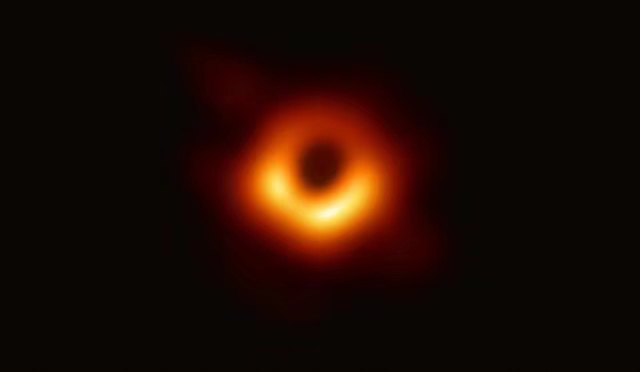
\includegraphics[width=13cm]{./Pictures/intro_black_hole.jpg}
	\captionsetup{justification=centering}
	\caption{人类首张黑洞照片}
	\label{intro_black_hole}
\end{figure}

光通信技术正是CNGI的主干网基础,它不仅可以提供长距离的大带宽数据传输服务,随着大数据时代的到来,数据中心需要存储海量的数据,并且各个机柜之间以及芯片与芯片之间需要进行大量的数据传输,在不远的将来,光互联技术将迈向最后一步进入到处理器内部进行数据的传输与处理。图\ref{intro_siliconphotonics}展示了电互联、硅基光通信和光纤通信在不同工作距离下的适用范围。当数据的通信速率达到10~GBps以上时,利用金属的电互联技术将会因为损耗、串扰与功耗等问题没法正常工作。而利用光互联技术,可以实现大带宽、低功耗和低时延的数据传输。因此,在信息传输领域,光子器件具有无可替代的地位。

\begin{figure}[htb]
	\centering
	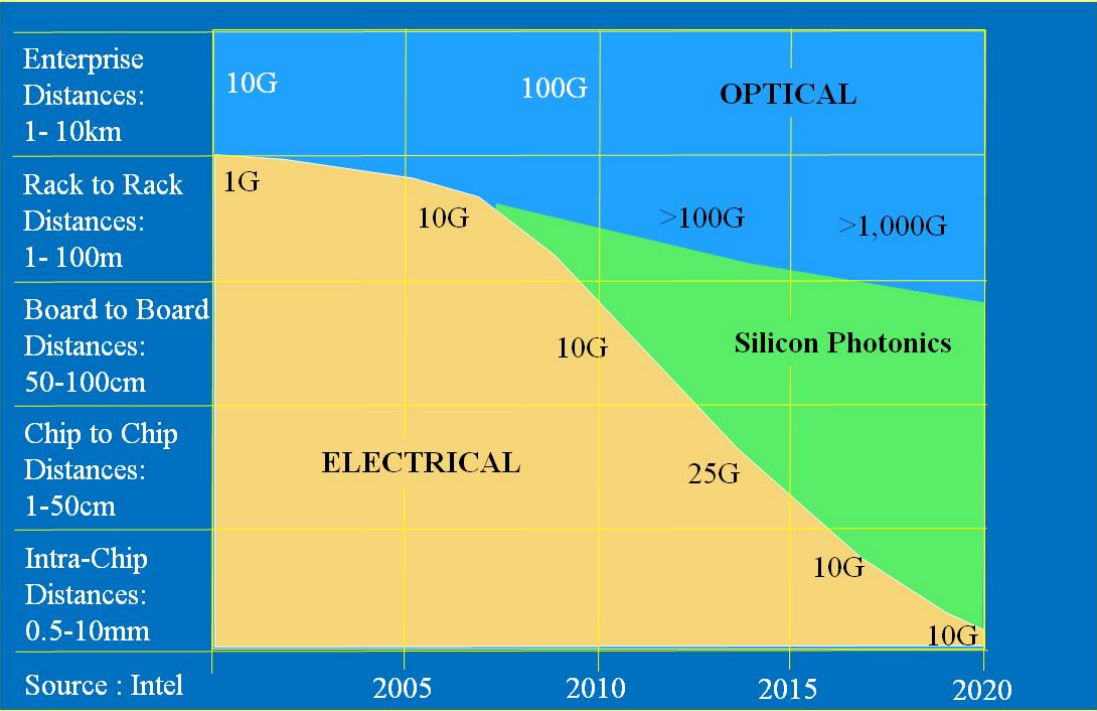
\includegraphics[width=13cm]{./Pictures/intro_siliconphotonics.png}
	\captionsetup{justification=centering}
	\caption{电互联、硅基光通信和光纤通信在不同通信距离下的适用范围\cite{zuffada2012industrialization}}
	\label{intro_siliconphotonics}
\end{figure}

传统光通信器件,由于价格高,尺寸大,功耗大已经无法满足芯片间以及芯片内部的应用,因此近几十年来,研究人员不断尝试新的材料平台,新的结构来实现大带宽、低功耗、低成本的解决方案。受到电子集成电路技术的启发,1969年,贝尔实验室的Stewart E. Miller提
出了集成光学的概念\cite{miller1969integrated},在片上集成激光器、调制器等光路系统代替组合式光路,利用器件的小型化可以避免热、机械、声等环境因素的影响,由此光互联技术进入了崭新的时代。

本章将首先简要介绍集成光学,然后介绍其中最有潜力的硅基光电子集成技术,接着着重讨论在硅基光电子集成技术中的一种重要光源---混合集成DFB激光器,最后介绍由作者制作的硅基混合集成自脉冲DFB激光器及其在三个领域的应用。


\section{集成光学简介}

集成光学的发展的动力首先来自于光通信的发展,作为信息载体,光子相比于电子具有独特的优势。例如,光子不带电荷,因而其传输过程中无电磁串扰的问题;光子具有频率、相位、振幅、偏振参数可以用于调制和检测,为通信提供了更多的可能性。

与传统的分立光学器件相比,集成光子器件的优势有:
\begin{enumerate}[(1)]
	\item 
	没有了传统光学器件的对准和光束准直问题,整个系统集成到同一块芯片上,稳定性更好;
	\item
	缩小了光学系统的体积,能够实现片上实验室(Lab on a Chip),提高了光学器件的密度,降低了总的功耗,使用也更加方便;
	\item 
	可以利用已经成熟的CMOS加工工艺,实现低成本、大规模的自动化生产。
\end{enumerate}

随着新材料的不断研发,集成光学所使用的材料也日益多样化,我们可以根据光波导所使用材料平台的不同,将集成光器件平台分为以下几种类型:

\begin{enumerate}[(1)]
	\item 
	掺杂型二氧化硅(SiO\SB{2})波导平台~~~~二氧化硅是最早被广泛采用的光波导材料之一,也是目前为止发展最成熟的无源器件平台。为了构成波导,至少要有两种折射率差的材料构成波导的芯层与包层,通常采用的办法是:在波导芯层中掺杂硼(P)、锗(Ge)等材料,使得其折射率比包层高大约1\%。由于折射率差比较小,故其波导尺寸较大,因此与早期的光通信中的光纤模式比较匹配,方便耦合,得到了广泛的应用。但也正是因为其波导尺寸比较大,不利于提高集成度,且二氧化硅属于无源材料,无法用其制作激光器、调制器、探测器等有源器件,也限制了其的应用。
	\item 
	聚合物波导平台~~~~聚合物材料是新近发展起来用于光电子器件领域的材料。该类波导的热光系数与电光系数都比较大,通过外场极化的方法可以获得高于LiNbO\SB{3}等无机晶体的电光系数,非常适合用于制作光开关与光调制器等器件。聚合物波导还具有材料配置方便、成本低廉等优点,只需要通过旋涂聚合物材料,曝光显影就能够制作,且工艺与半导体工艺相兼容,具有很好的发展前景。此外,几乎任何材料都可以作为聚合物的衬底,方便了聚合物与其他材料的集成。但是另一方面,聚合物材料容易老化,可靠性较差,这不利于提高器件的稳定性,且大部分聚合物无法承受较高的温度,不适用于CMOS工艺的大规模生产。
	\item 
	绝缘体上硅(silicon-on-insulator, SOI)波导平台~~~~绝缘体上硅材料是一种广泛用于制作集成电路的材料,利用现有的CMOS加工工艺,硅光集成芯片加工成本低,能够实现大规模生产。同时,硅材料具有优异的光学、电学和热学性能,硅材料在1.1~$\mu m$\~{}7~$\mu m$波段的光损耗很低,其氧化物SiO\SB{2}的折射率为1.46@1550 $nm$,与其本身折射率3.455@1550 $nm$相差很大,非常适合作为包层,能够对光形成很强的束缚,实现亚微米尺寸的波导。绝缘体上硅平台唯一不足的是,硅是一种间接带隙材料,无法实现高效率地发光,同时硅的电光效应较弱,故也无法制作高性能的电光调制器,由于其对通信波段的光没有吸收,故也无法制作探测器。研究人员们也找到了很多办法来解决绝缘体上硅平台的这些问题,比如通过混合集成的办法集成激光器与调制器\cite{ma2017demonstration,fang2006electrically},利用等离子体色散效应来实现速度达到10~Gbps以上的光调制器\cite{manipatruni2007high,fujikata201025,xiao201360}。
	\item 
	氮化硅(Si\SB{3}N\SB{4})波导平台~~~~氮化硅作为一种CMOS工艺中常用的掩模材料,近年来其优良的光学性能逐渐被人们发现并利用\cite{moss2013new}。氮化硅材料拥有比硅平台更低的损耗,以及较强的二阶非线性效应,因此在非线性研究领域受到了广泛的关注。氮化硅的低损耗窗口还包括可见光波段,且其有较高的折射率,故在可见光波段器件方面具有非常重要的应用。氮化硅还具有可调的色散特性,使其在光通信领域也有重要的应用。其缺点与绝缘体上硅平台类似,即也无法直接在其上制作有源器件,需要用混合集成技术才能实现。
	\item
	III-V族波导平台~~~~III-V族材料由于其直接带隙特性,通过调节不同元素的比例,其发光光谱可以从可见光一直到红外波段,能够满足照明、通信等方面的各种需求。III-V族材料可以实现光源、光放大器、调制器、探测器、波分复用器等器件,是作为光通信的理想材料。但是,由于III-V材料不易制做大尺寸的晶圆,加工成本较高,产品良率较低,使得其实现大规模商业化应用还有一定的困难。
	\item 
	铌酸锂(LiNbO\SB{3}波导平台~~~~LiNbO\SB{3}是一种比较成熟的多功能晶体,得益于其具有线性电光效应(Pockel effect, 普克尔效应),是制作电光调制器非常好的材料。LiNbO\SB{3}材料常通过掺杂来形成折射率差构成光波导,基于LiNbO\SB{3}的分立器件已经得到广泛应用。近年来,由于铌酸锂单晶薄膜的成功开发,其在集成领域的应用也开始崭露头角\cite{wang2018integrated,he2019high}。
\end{enumerate}

\begin{figure}[htb]
	\centering
	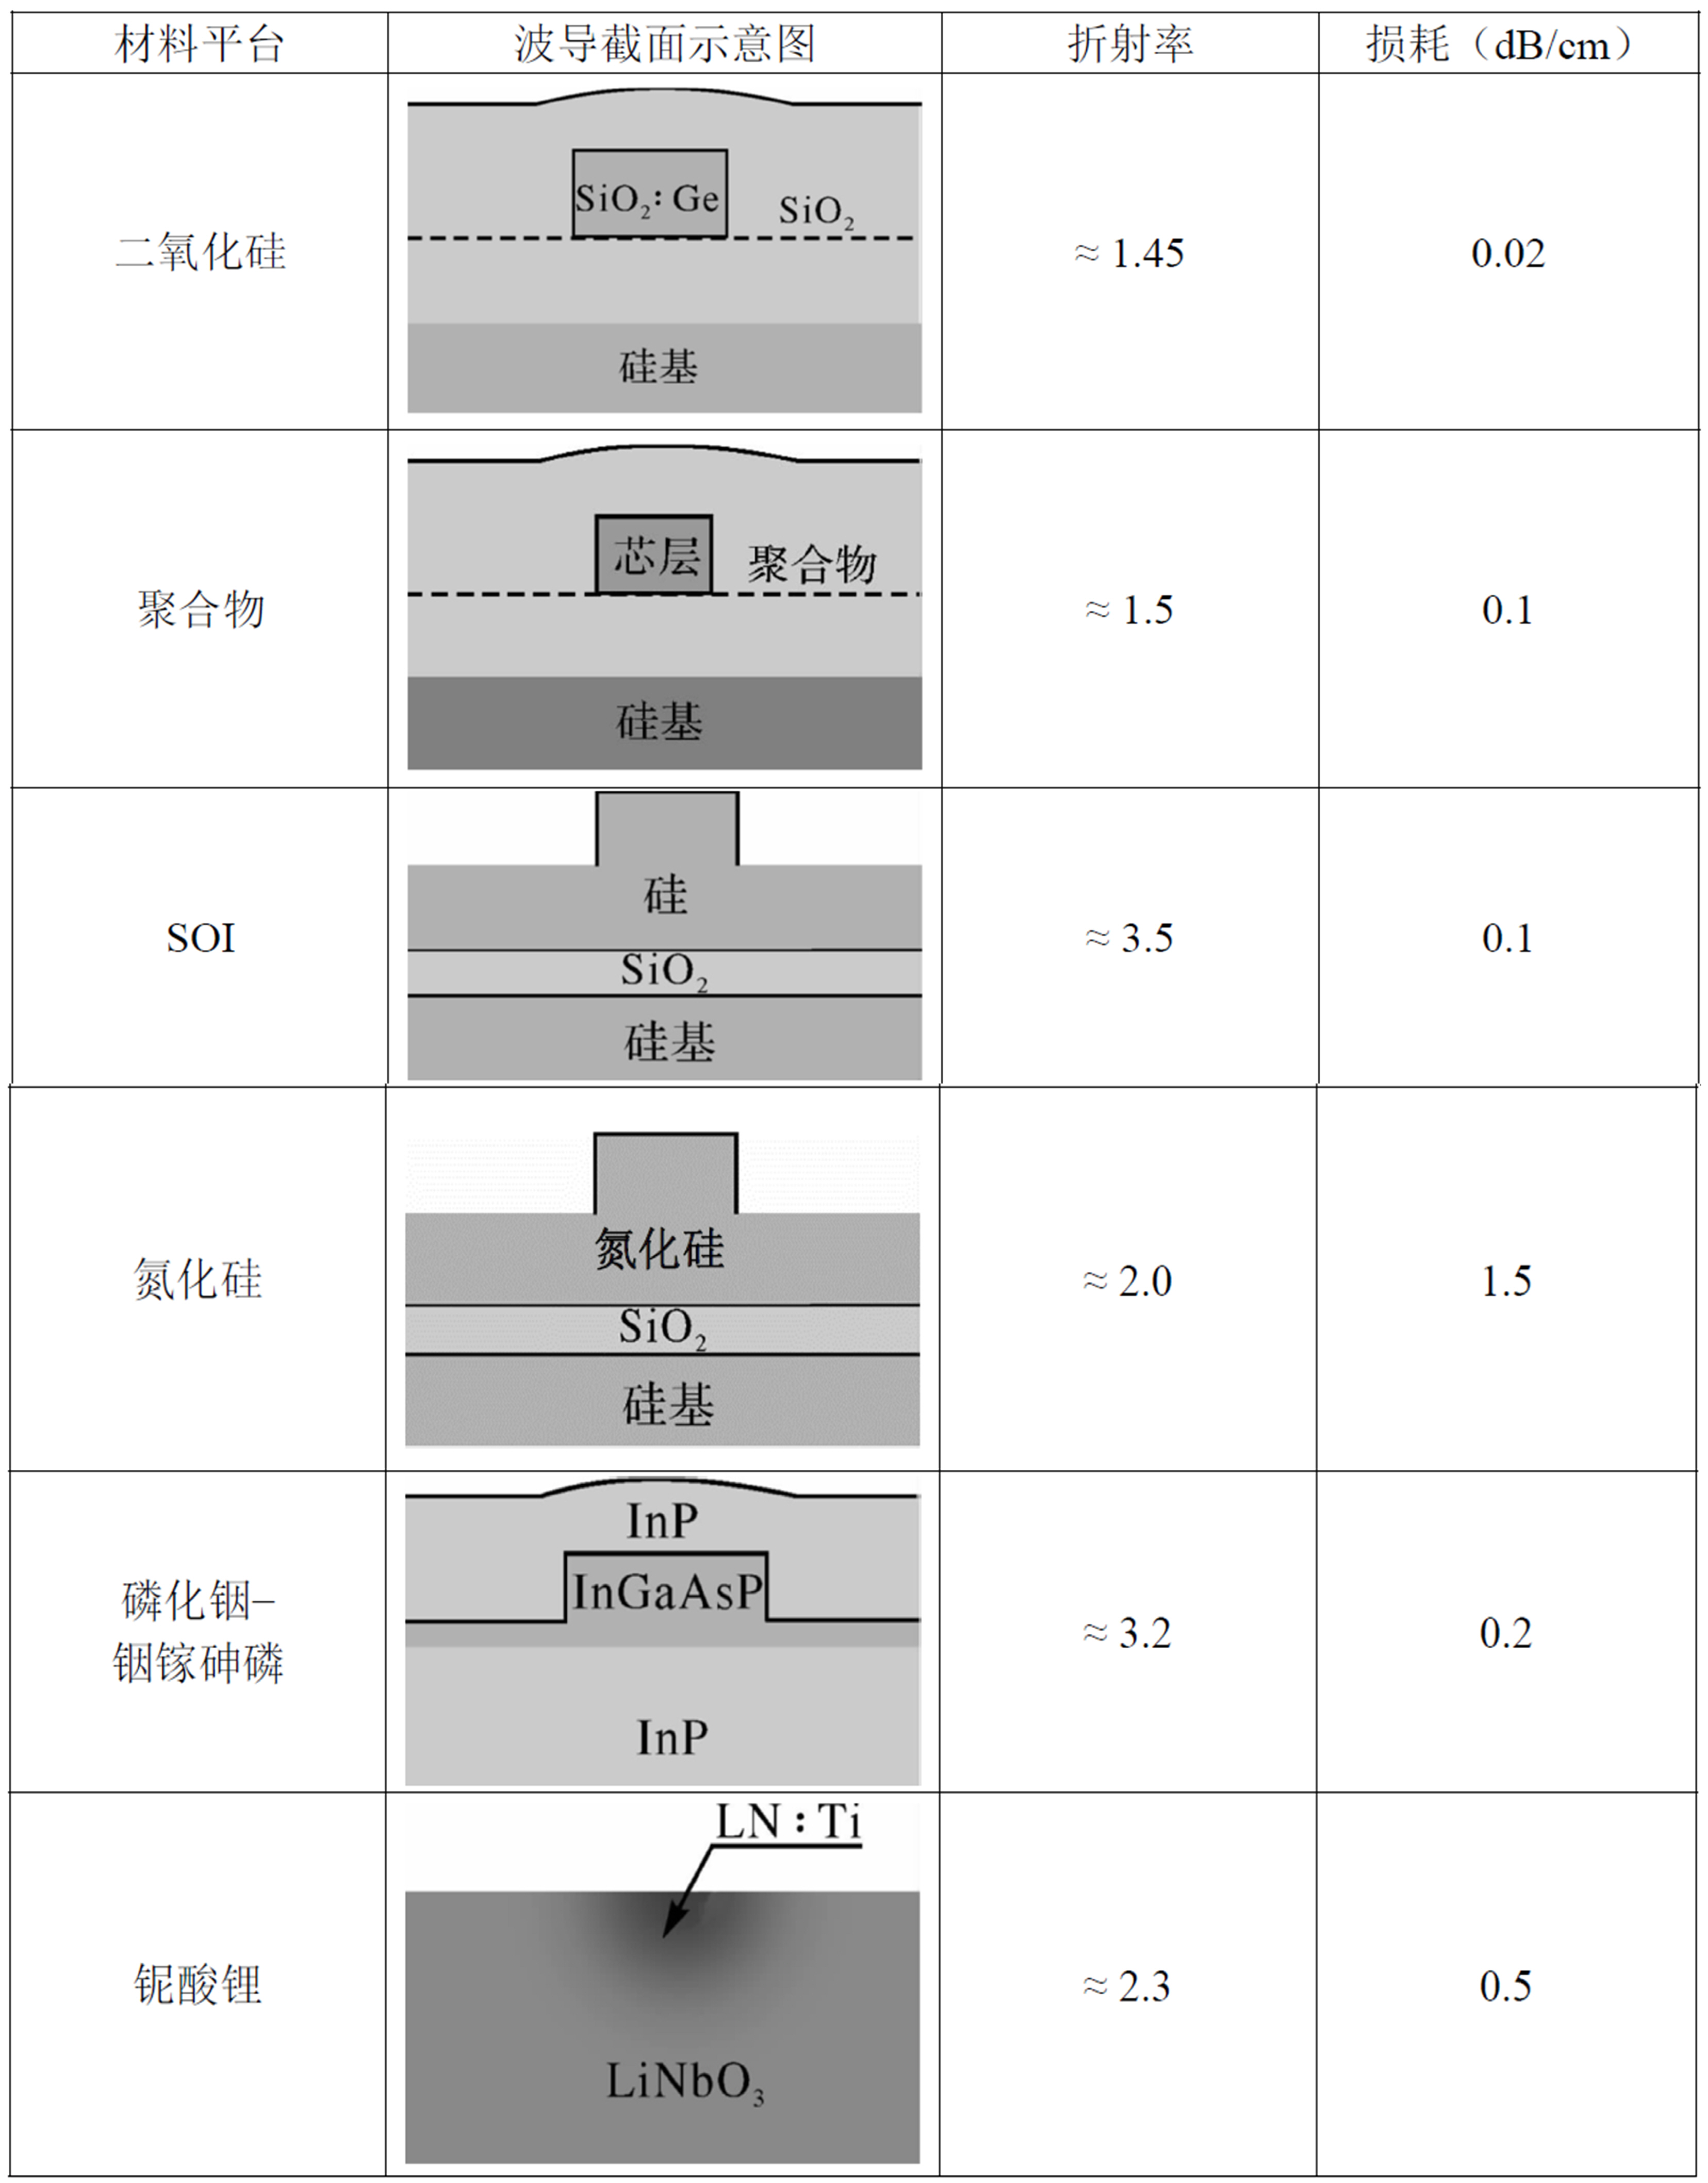
\includegraphics[width=13cm]{./Pictures/intro_materialplatform.jpg}
	\captionsetup{justification=centering}
	\caption{不同材料平台光波导平台\cite{hslwngzjc}}
	\label{intro_materialplatform}
\end{figure}

图\ref{intro_materialplatform}总给出了以上几种材料平台的波导结构以及其在通信波长λ@1550 $nm$的折射率和损耗。如上所述,各个平台都有相应的缺点与优点。在集成光学刚发展起来时,因为集成规模较小而更多的使用分立器件,往往根据器件的功能需求,选择最佳的平台以实现最佳的性能,比如,制作分立的激光器,往往利用III-V族材料平台,分立的调制器,往往采用铌酸锂(LiNbO\SB{3})波导平台。但是随着集成光学的发展,高密度的集成越来越受到关注,绝缘体上硅平台由于芯层与包层之间折射率差达到58\%,能够实现非常好的光限制,使得该平台成为高密度集成光学芯片的最好选择。

\section{硅基光电子集成技术}

硅基光子学最大的优势在于其制作工艺与当今非常成熟的CMOS(complementary metal-oxide semiconductor)工艺相兼容,且由于其特征尺寸远远大于晶体管的特征尺寸,故可以利用淘汰的CMOS生产线来制作硅基光电子器件,实现大规模自动化生产,制作成本大大降低,故硅基光子学已经被广泛认为是下一代通信技术的关键。

1985年,基于SOI平台的波导结构首次被研究并使人们意识到集成硅基光电子集成技术的潜力\cite{soref1985single,reed2005silicon}。不久之后的1989年,Bookham技术公司就开始将硅波导实现商业化。20世纪90年代,Bookham技术公司研发了最早的硅光集成器件芯片-硅光芯片与光纤结合的陀螺仪与压力传感器芯片\cite{rickman2014commercialization};随后,硅基光子学的产业化方向逐渐转向光通信中的波分复用器件(wavelength-division-multiplexing, WDM),因为利用波分复用技术,可以大大提升光纤的通信容量。随着基于硅波导的p-i-n调制器与锗硅探测器和调制器的实现\cite{liu2005tensile,feng2014micron},在通信领域采用硅基光子学变得越来越有希望。Luxtera、Mellanox和Acacia等公司已经成功开发了基于硅基集成技术的100~Gbps的光收发模块和相干收发模块,并朝着200~Gbps和400~Gbps迈进\cite{boeuf2015recent,feng2014micron,doerr2014single},国内的旭创科技、光迅科技、海信宽带等则已经可以提供400~Gbps的收发模块,这些收发模块将用于提升超级计算机、和电信通信领域等的性能。

\begin{figure}[htb]
	\centering
	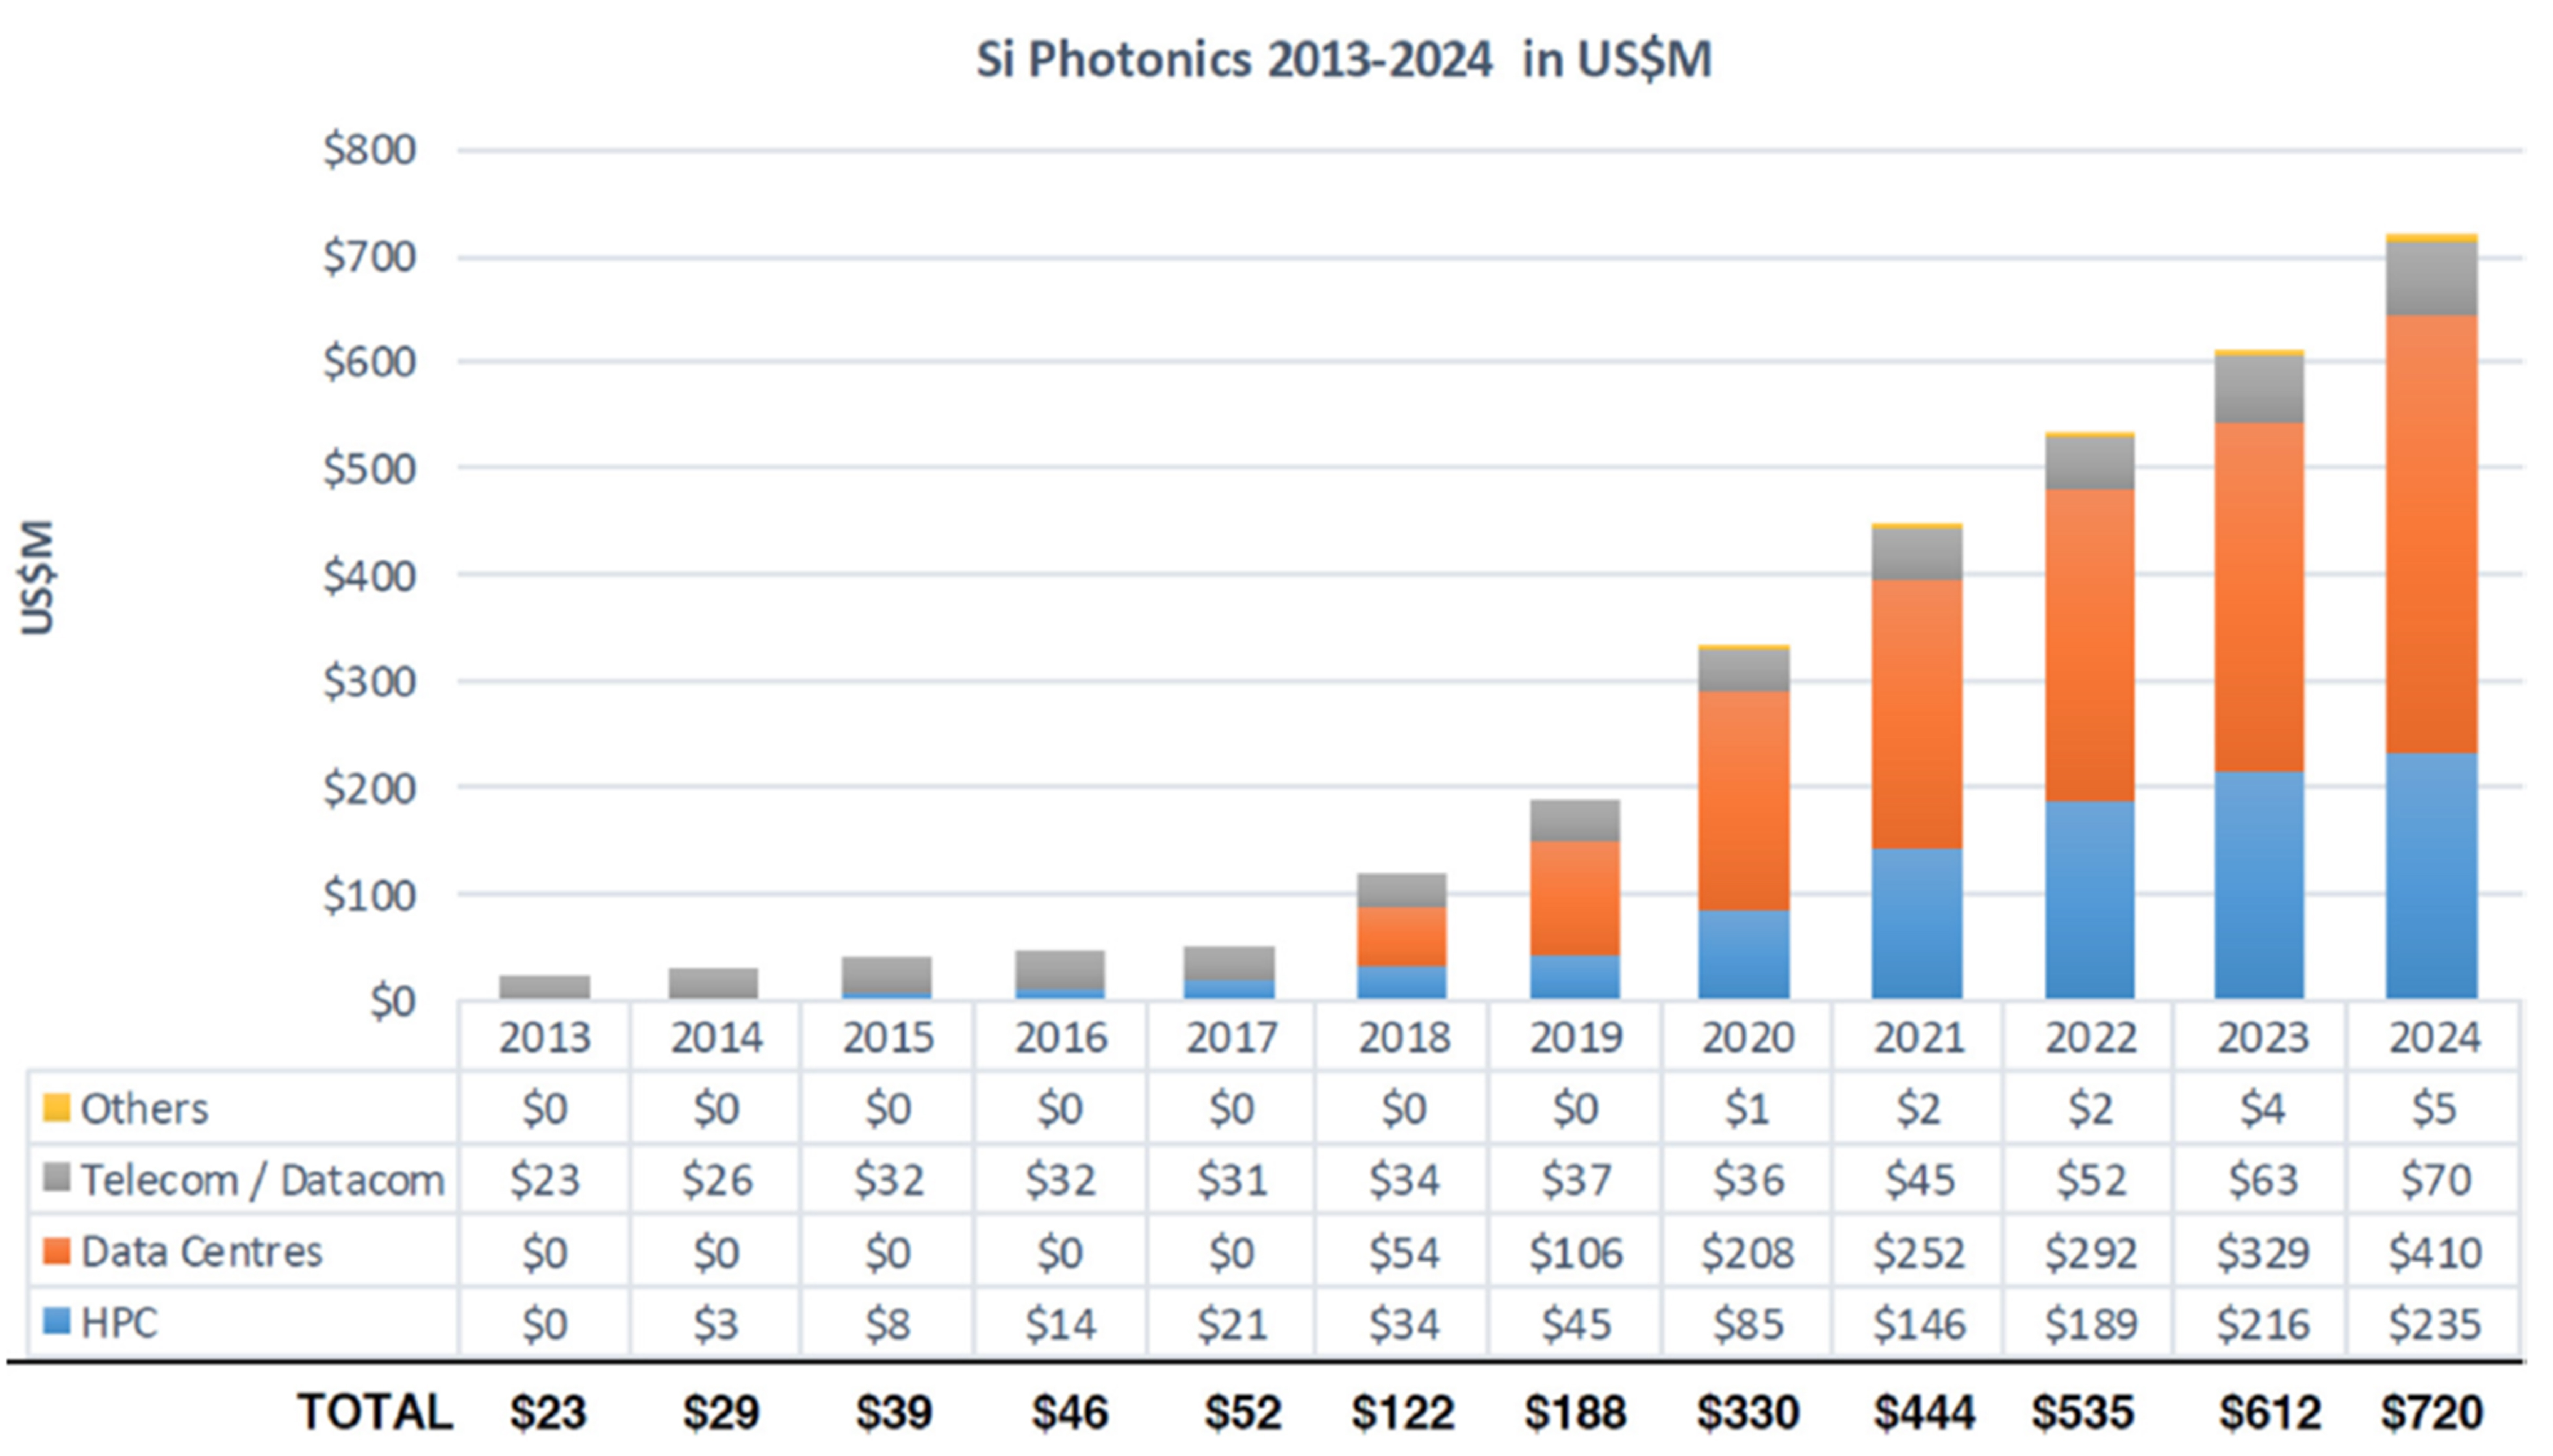
\includegraphics[width=14cm]{./Pictures/intro_siliconphotonicsmarket.jpg}
	\captionsetup{justification=centering}
	\caption{市场咨询机构Yole Développement对2013年至2024年硅光芯片市场的预测(来源:Silicon Photonics Report - Yole Développement; ‘Emerging optical data centers from big Internet companies (Googlem Facebook, ...) will be triggering the market growth in 2018...’ )}
	\label{intro_siliconphotonicsmarket}
\end{figure}

图\ref{intro_siliconphotonicsmarket}是市场咨询机构Yole Développement对2013年至2024年硅光芯片市场的统计与预测,2013年至2017年,硅光芯片主要用于电信和超级计算机行业,总体市场规模较小,2018年,硅光芯片将开始腾飞并且在未来会保持20\%以上的高速增长,主要得益于硅光芯片可以将数据传输的成本降低到\$1/Gbps,相比于之前的电互联和多模光纤互联成本更低,所以数据中心和超级计算机行业将会大规模部署。除了费用更低外,硅光芯片能耗也可以降低到pJ/bit量级,器件的稳定性也更好。

在典型的光互联系统中,最重要的组成部分就是光收发模块,其由发射机与接收机两部分组成,如图\ref{intro_transceiver}所示。在发射机中,经过CPU处理的数据通过调制器调制激光器的输出光,从而将所需要传输的数据加载到光波上。为了增加通信的容量,可以采用波分复用技术,将不同路的信号加载到不同波长的激光上。调制的方式可以采用直接调制或者外调制,直接调制是指通过调制激光器的驱动电流来调制激光器的输出光强,外调制则是通过外接调制器来对激光器的输出光强进行调制。直接调制的优点是简单方便,但是由于调制时会改变激光器的载流子浓度,会出现频率啁啾效应,调制速率受限。外调制虽然所需要用到的调制器结构较为复杂,但具有良好的调制性能,由其是在高速率的状态下。

\begin{figure}[htb]
	\centering
	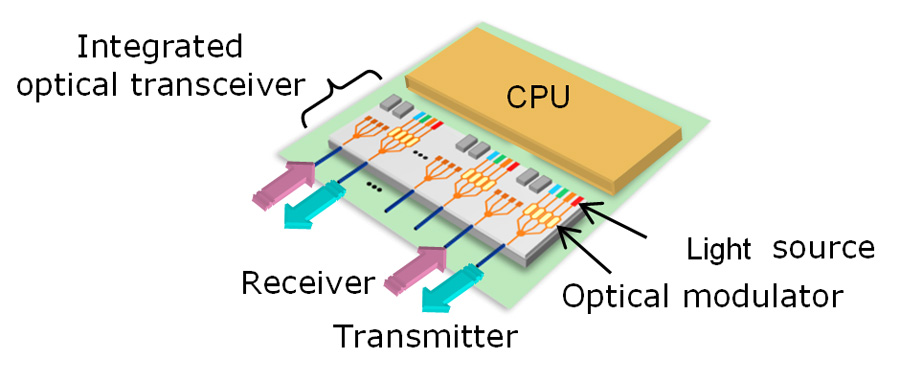
\includegraphics[width=14cm]{./Pictures/intro_transceiver.jpg}
	\captionsetup{justification=centering}
	\caption{光收发模块示意图(Fujitsu)}
	\label{intro_transceiver}
\end{figure}

无论是直接调制还是外调制,都需要有能够在片上集成的高效单模激光器,但是由于硅的间接带隙特性,其发光效率特别低,虽然研究人员已经利用拉曼效应(Raman scattering)和布里渊效应(Brillouin scattering)成功制作了硅基激光器\cite{otterstrom2018silicon,rong2007low},但该类激光器都需要采用光泵浦的方式,不适合大规模用于光互联通信系统中,要利用硅制作高效地电泵浦激光器仍然非常困难。

\begin{figure}[htb]
	\centering
	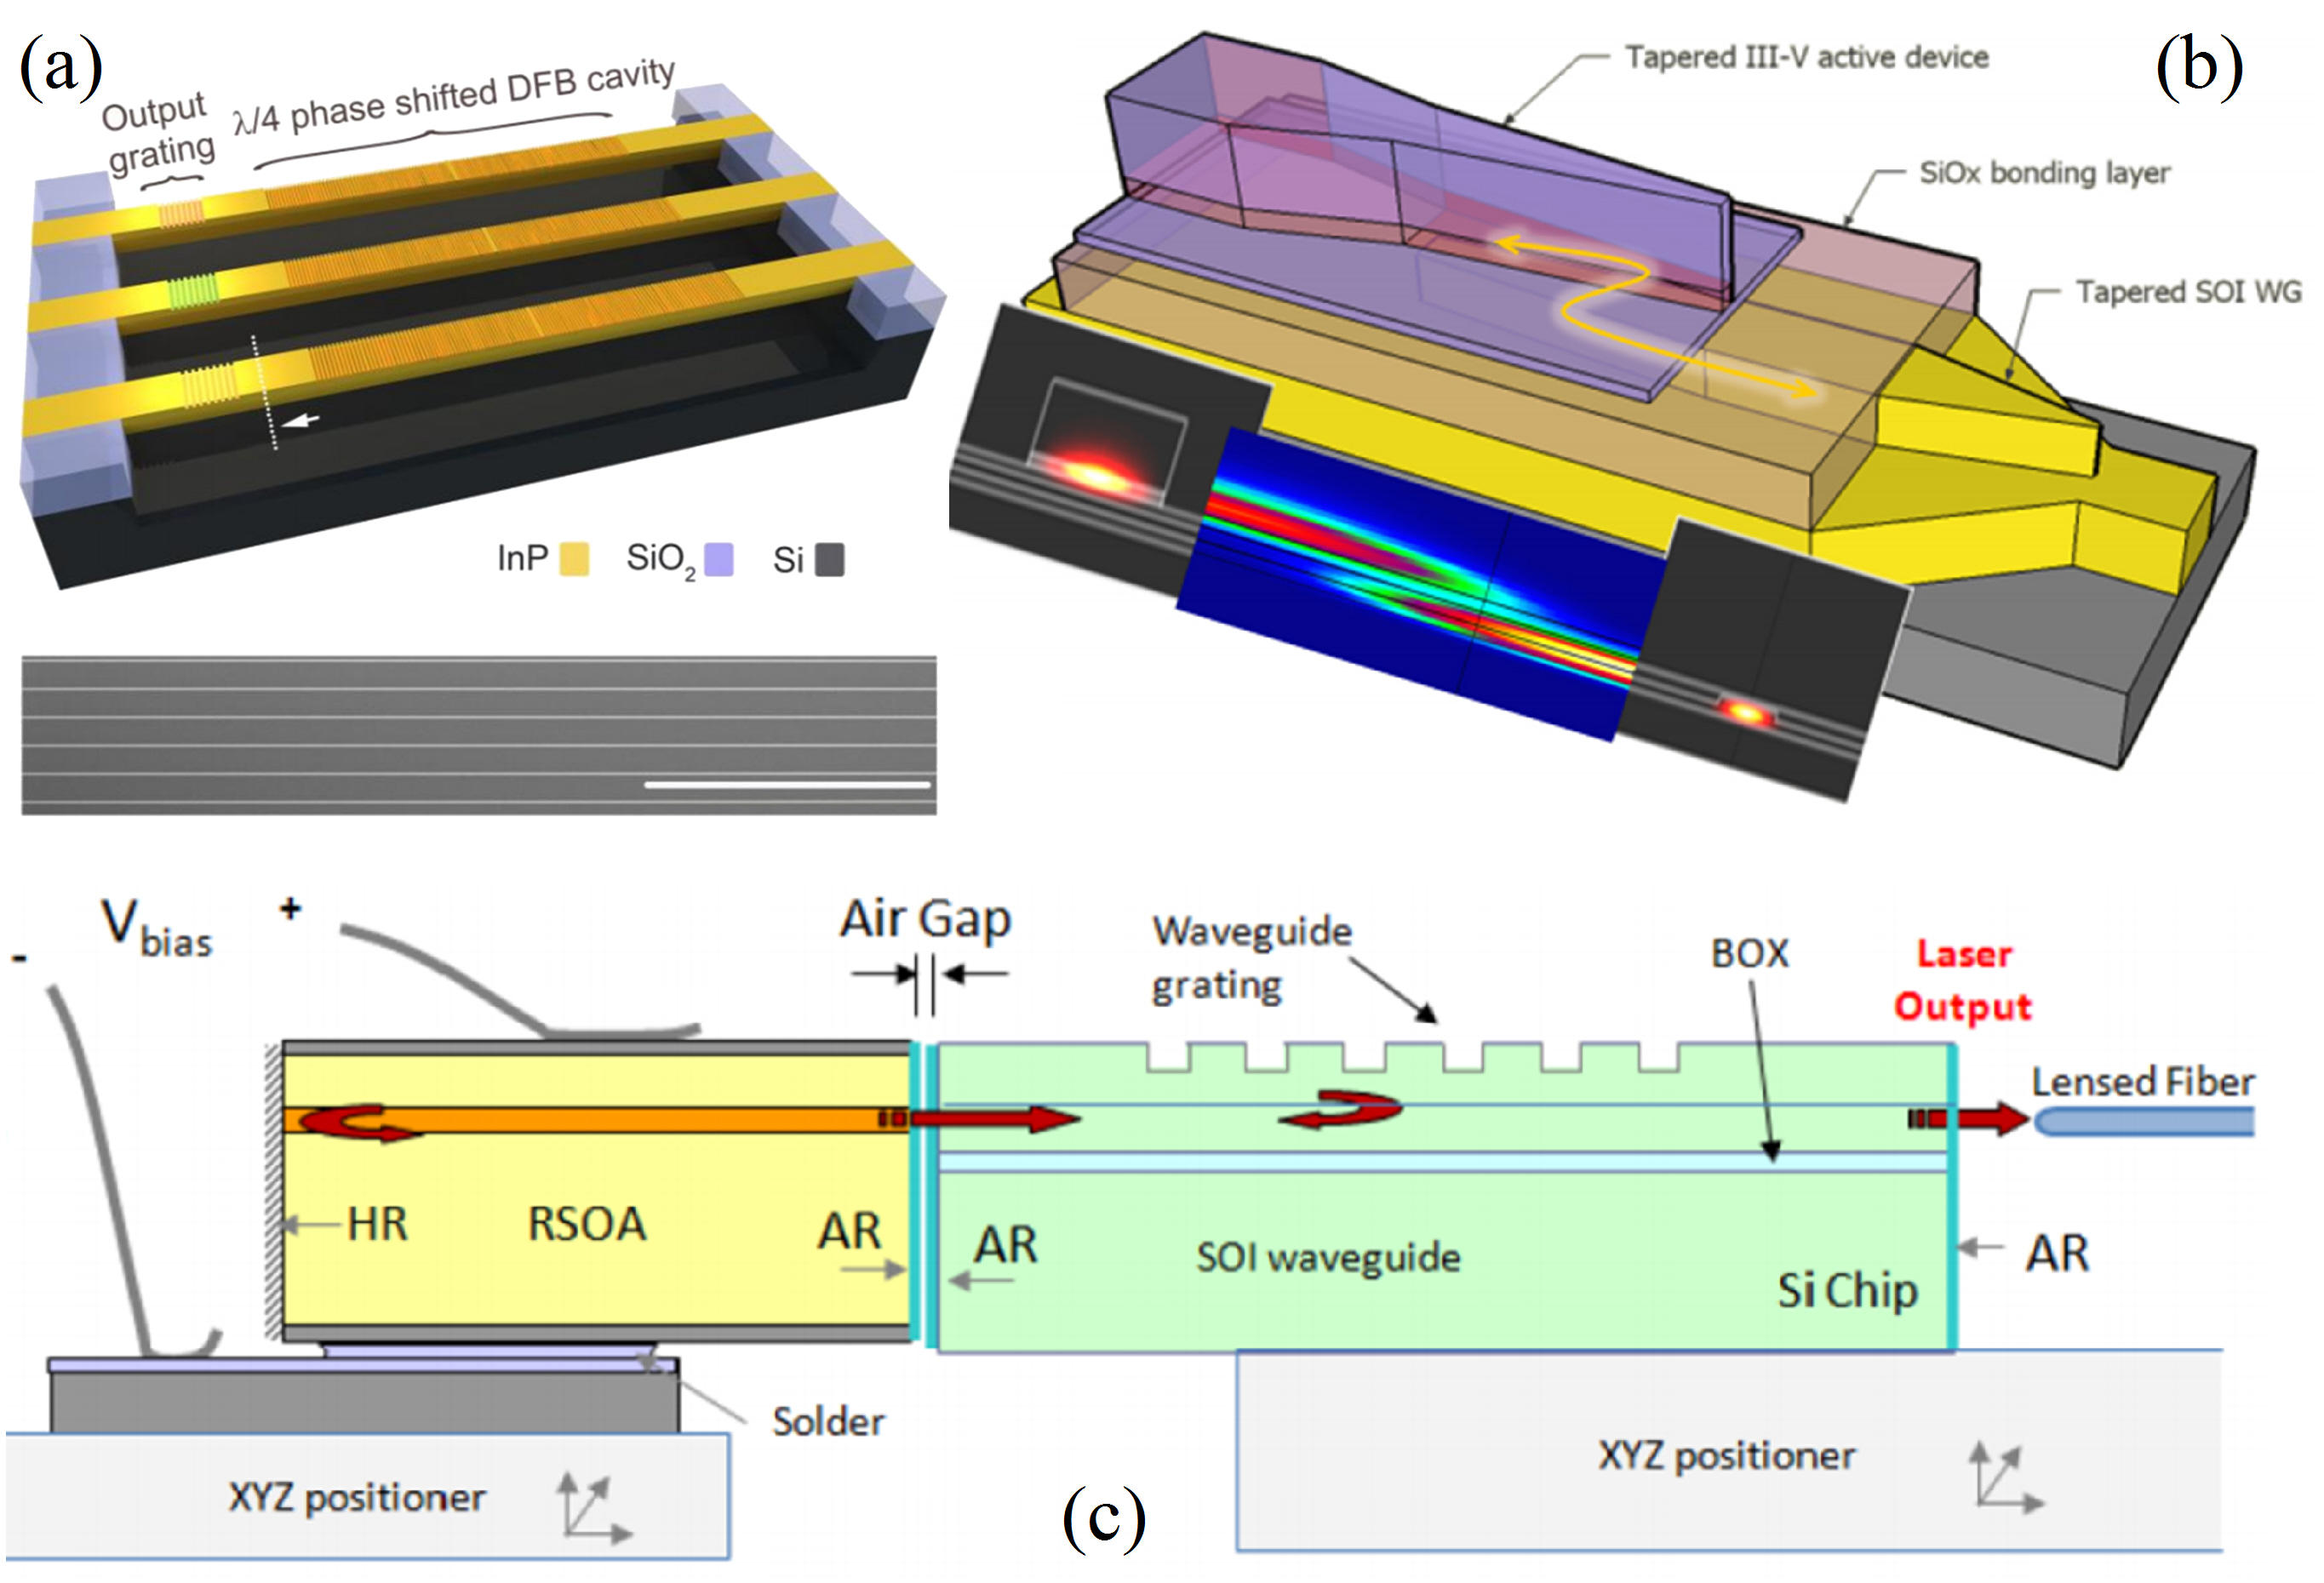
\includegraphics[width=14cm]{./Pictures/intro_lasers.jpg}
	\captionsetup{justification=centering}
	\caption{三种硅基集成激光器的方案:(a)在硅上外延生长IIII-V材料制作的激光器\cite{wang2015room};(b)~III-V材料与硅键合制作的激光器\cite{keyvaninia2013demonstration};(c)~III-V有源增益区与硅器件通过Flip-Chip键合制作的激光器\cite{zilkie2012power}}
	\label{intro_lasers}
\end{figure}

由于无法利用硅材料在片上实现高效的电泵浦激光器,人们想到了利用III-V族有源增益材料与硅结合的方法来制作硅上的光源\cite{heck2013hybrid,keyvaninia2013heterogeneously},一般有三种方式来实现硅与III-V族材料的集成\cite{bowers2014path}。第一种方法是直接在硅层上面生长III-V族外延层,由于硅与III-V族材料的晶格与热膨胀系数不匹配(Si与InP有8\%的晶格常数不匹配度,84\%的热膨胀系数不匹配度),通常会使用锗作为中间缓冲层来释放晶格不匹配造成的应力。图\ref{intro_lasers}(a)所示为Wang等人通过在硅波导上利用羟化四甲铵腐蚀液(TMAH)腐蚀出V型凹槽,通过选择性生长的方法,可以将因晶格不匹配产生的线位错与反相面限制在20~$nm$厚度内,故不会影响III-V族材料制作的激光器的性能\cite{wang2015room},但是该激光器还是需要光泵浦而不是电泵浦,因此不适用于片上大规模应用;第二种是利用键合的方法,将III-V晶片先键合到硅波导上,这一步不需要精确的对准,键合完之后在III-V晶片上制作激光器的结构,硅波导与III-V波导的光通过垂直耦合的方式进行耦合。图\ref{intro_lasers}(b)所示为Keyvaninia等人利用BCB作为键合层,将III-V族材料键合到SOI上提供增益,利用SOI上的腔结构提供反馈,制作的电泵浦激光器,在20~$^{\circ}$C条件下可以实现最大输出功率为10~$mW$\cite{keyvaninia2013demonstration};第三种是采用Flip-Chip的方法实现III-V族材料波导与硅波导的端面耦合,通过III-V族材料提供增益,硅波导上的谐振腔提供反馈,实现激光的输出。图\ref{intro_lasers}(c)所示为Zilkie等人利用半导体放大器(SOA)与硅波导DBR反射镜,通过Flip-Chip的方法实现端面耦合,制作的激光器最大输出功率为6~$mW$\cite{zilkie2012power}。

目前,考虑到直接外延生长III-V族材料制作的激光器由于缺陷的影响寿命比较短\cite{liu2015reliability,sun2016room},主要采用硅与III-V族材料键合的方式来制作片上激光器(heterogeneous integration)。这样可以充分利用两者的优势,III-V材料具有直接带隙材料的特点,可以提供较高的增益,而且能带间隔可以通过不同组分的含量进行调节,实现不同波长的激射;硅基光子平台可以在通讯波段提供低损耗的波导(<1~dB/$cm$),而且由于其超高的折射率差可以实现较小的波导弯曲,实现高密度的集成。目前,基于硅基光子平台的无源器件已经被大量的制作完成,包括阵列波导光栅(AWG),刻蚀衍射光栅(EDG),多模干涉器(MMI),微环谐振腔,耦合光栅等等\cite{asghari2011silicon,jalali2006silicon},可以实现片上光传输的种种功能。利用键合的方式将III-V材料与SOI混合集成,研究人员已经实现了在SOI上的电泵浦激光器,高速调制器、探测器和半导体光放大器\cite{liang2010hybrid,roelkens2010iii,liang2010recent,duan2014hybrid}。

在混合集成激光器中,DFB激光器(distributed feedback laser)由于其稳定的单模特性,工艺简单,性能优良而被广泛采用。

\section{硅基III-V混合集成DFB激光器}

DFB激光器也叫分布反馈式激光器,是一种在光收发模块中常用的端面出射激光器,与另一种常用的DBR激光器(distributed brag reflector laser)不同的是,其布拉格反射光栅位于激光器的腔内,如图\ref{intro_dfb_laser}所示。布拉格光栅可以位于包层作为折射率实部的调制,叫做折射率耦合;也可以位于增益材料中作为折射率虚部的调制,叫做增益耦合。它们在实际激光器制作过程中的区别是,是否需要$\Lambda/2$的相移来实现单模激射($\Lambda$为布拉格光栅的周期)。布拉格光栅的周期需要经过设计使其反射波长位于增益介质的增益带宽内,在光通信波段,常用的增益介质为基于InP的三元或者四元外延结构,如InGaAsP和InGaAlAs。

\begin{figure}[htb]
	\centering
	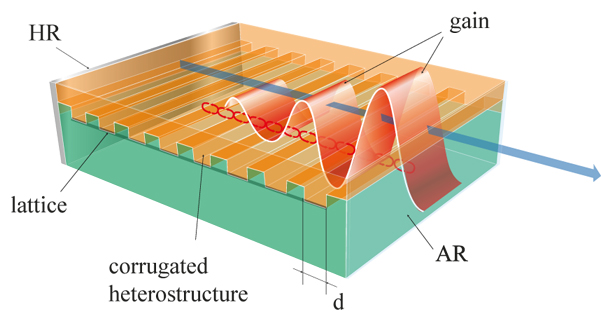
\includegraphics[width=11cm]{./Pictures/intro_dfb_laser.jpg}
	\captionsetup{justification=centering}
	\caption{DFB激光器示意图,AR: antireflection, HR: high reflection}
	\label{intro_dfb_laser}
\end{figure}

本文所研究的混合集成DFB激光器如图\ref{intro_heterogeneously_dfb_laser}所示,DFB光栅制作在SOI的硅上,光栅采用一阶光栅,以InGaAsP材料作为有源层的III-V芯片通过BCB键合到硅波导上,之后通过结合光刻与干法刻蚀或湿法刻蚀完成III-V波导的制作。硅波导与III-V波导之间的光通过反向锥形波导结构进行耦合,使得从有源区产生的激光通过硅波导上的耦合光栅输出,进行测试。通过控制BCB的厚度,可以控制光栅的耦合强度,从而提供了一种可以控制激光器性能的维度,比如可以通过增加BCB的厚度减少光在III-V波导中的比例来减小激光器的线宽\cite{yariv2016rethinking}。

\begin{figure}[htb]
	\centering
	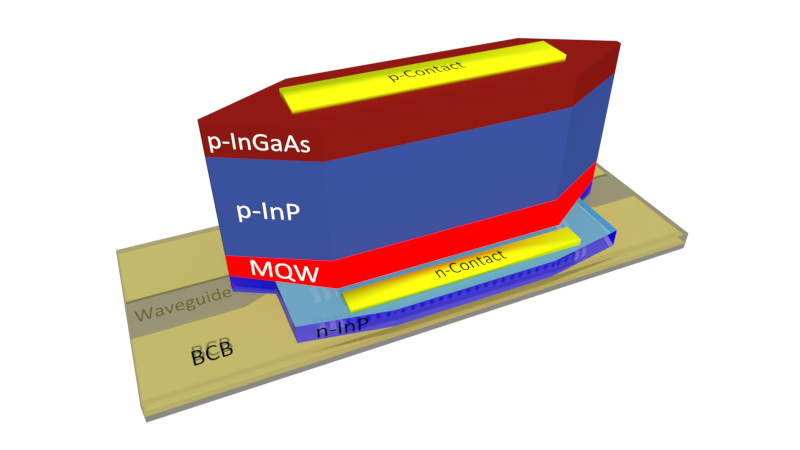
\includegraphics[width=15cm]{./Pictures/intro_heterogeneously_dfb_laser.png}
	\captionsetup{justification=centering}
	\caption{硅基III-V混合集成DFB激光器示意图}
	\label{intro_heterogeneously_dfb_laser}
\end{figure}

\section{DFB激光器的应用}

\subsection{微波光子领域的应用}

传统上微波信号是利用电子电路经过多级倍频来达到所需要的频率,然后通过同轴电缆进行传输,但是由于一些固有的和寄生的阻抗或者容抗限制,该种方法能够产生的微波信号频率与传输损耗都会受到限制,而且成本也较高。在过去三十多年来,微波光子学(microwave photonics, MWP)这门学科吸引了众多研究人员的注意,因为其可以将微波领域与光子学领域结合起来,实现在微波系统上实现起来特别复杂或者没法实现的功能。而且利用微波光子学,可以实现新的信息传输系统,实现微波信号的长距离低损耗传输\cite{capmany2007microwave,seeds2002microwave,seeds2006microwave,yao2009microwave}。其应用领域包括蜂窝天线,无线通信,卫星通信,有线电视,分布天线系统和医学成像等。

微波光子学最开始主要是利用分立的光电子器件和光纤来实现一些功能,比如微波信号的产生、分配、处理与分析,其器件昂贵笨重且不稳定,功耗也较大。随着硅基光电子集成技术的发展,微波光子学也开始朝着集成的方向发展,以实现低功耗与稳定的微波光子器件。

\begin{figure}[htb]
	\centering
	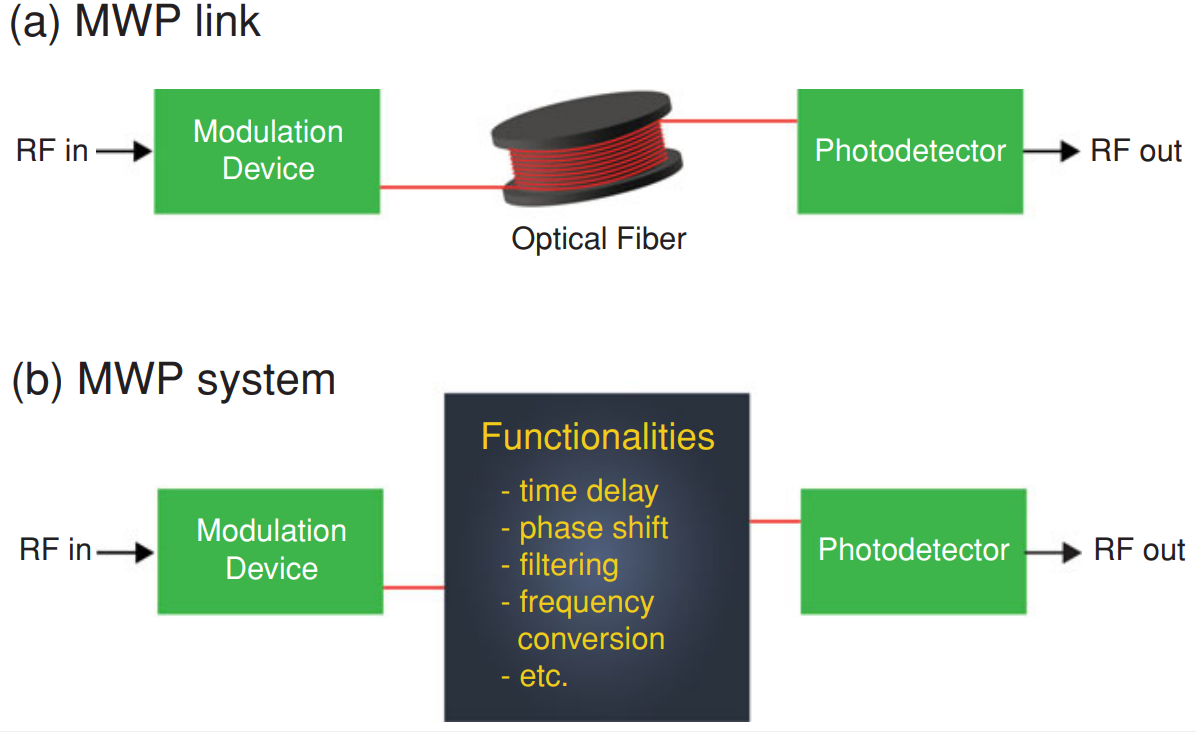
\includegraphics[width=14cm]{./Pictures/intro_mwp.png}
	\captionsetup{justification=centering}
	\caption{(a)典型的微波光子学链路示意图(b)简单的微波光子学系统组成示意图\cite{marpaung2013integrated}}
	\label{intro_mwp}
\end{figure}

图\ref{intro_mwp}(a)所示为典型的微波光子学链路示意图,微波信号经过调制器进行电光转换加载到光波上,经过光纤传输,然后探测器接收后光波之后将微波信号还原出来。图\ref{intro_mwp}(b)所示为典型的微波光子学系统示意图,微波信号经过调制器加载到光波上之后,可以在光频上进行时延,相移,滤波,频率转换等操作,然后再通过探测器转换到微波信号。利用光学方法进行处理可以实现更大的带宽,对不同的频率损耗均一,器件尺寸更小,不受电磁干扰影响,而且功耗也能够更低。

\subsection{光互联领域的应用}

外调制技术由于不会产生频率啁啾现象,可以减小光在光纤中传输的色散问题,使其对于需要经过光纤长距离传输的光通信系统来说相比于直接调制技术有明显的优势。但是对于短距离通信来说,直接调制相比于外调制有许多独特的优势。DFB激光器可以通过调制驱动电流大小来调制激光器的输出强度,这样一来,可以将光收发模块中的激光器与调制器融合成一个器件,可以降低系统的工艺复杂度,缩小总体器件的尺寸,还可以降低系统功耗。对于典型的马赫曾德外调制器,其往往需要较长的尺寸以换取较小的驱动电压,其尺寸往往达到数毫米。图\ref{intro_external_modulator}(a)所示为基于LiNbO\SB{3}的马赫曾德调制器,其长度为5~$mm$时,V$_{\pi}$为5.1~$V$,这对于调制速度要求不高但是对总体尺寸要求高的应用场景是不合适的。图\ref{intro_external_modulator}(b)所示基于III-V族材料的电吸收调制器,其插入损耗为5~dB,这意味着需要光源提供更高的功率来补偿调制器的损耗,从而导致整个系统的功耗增加。

\begin{figure}[htb]
	\centering
	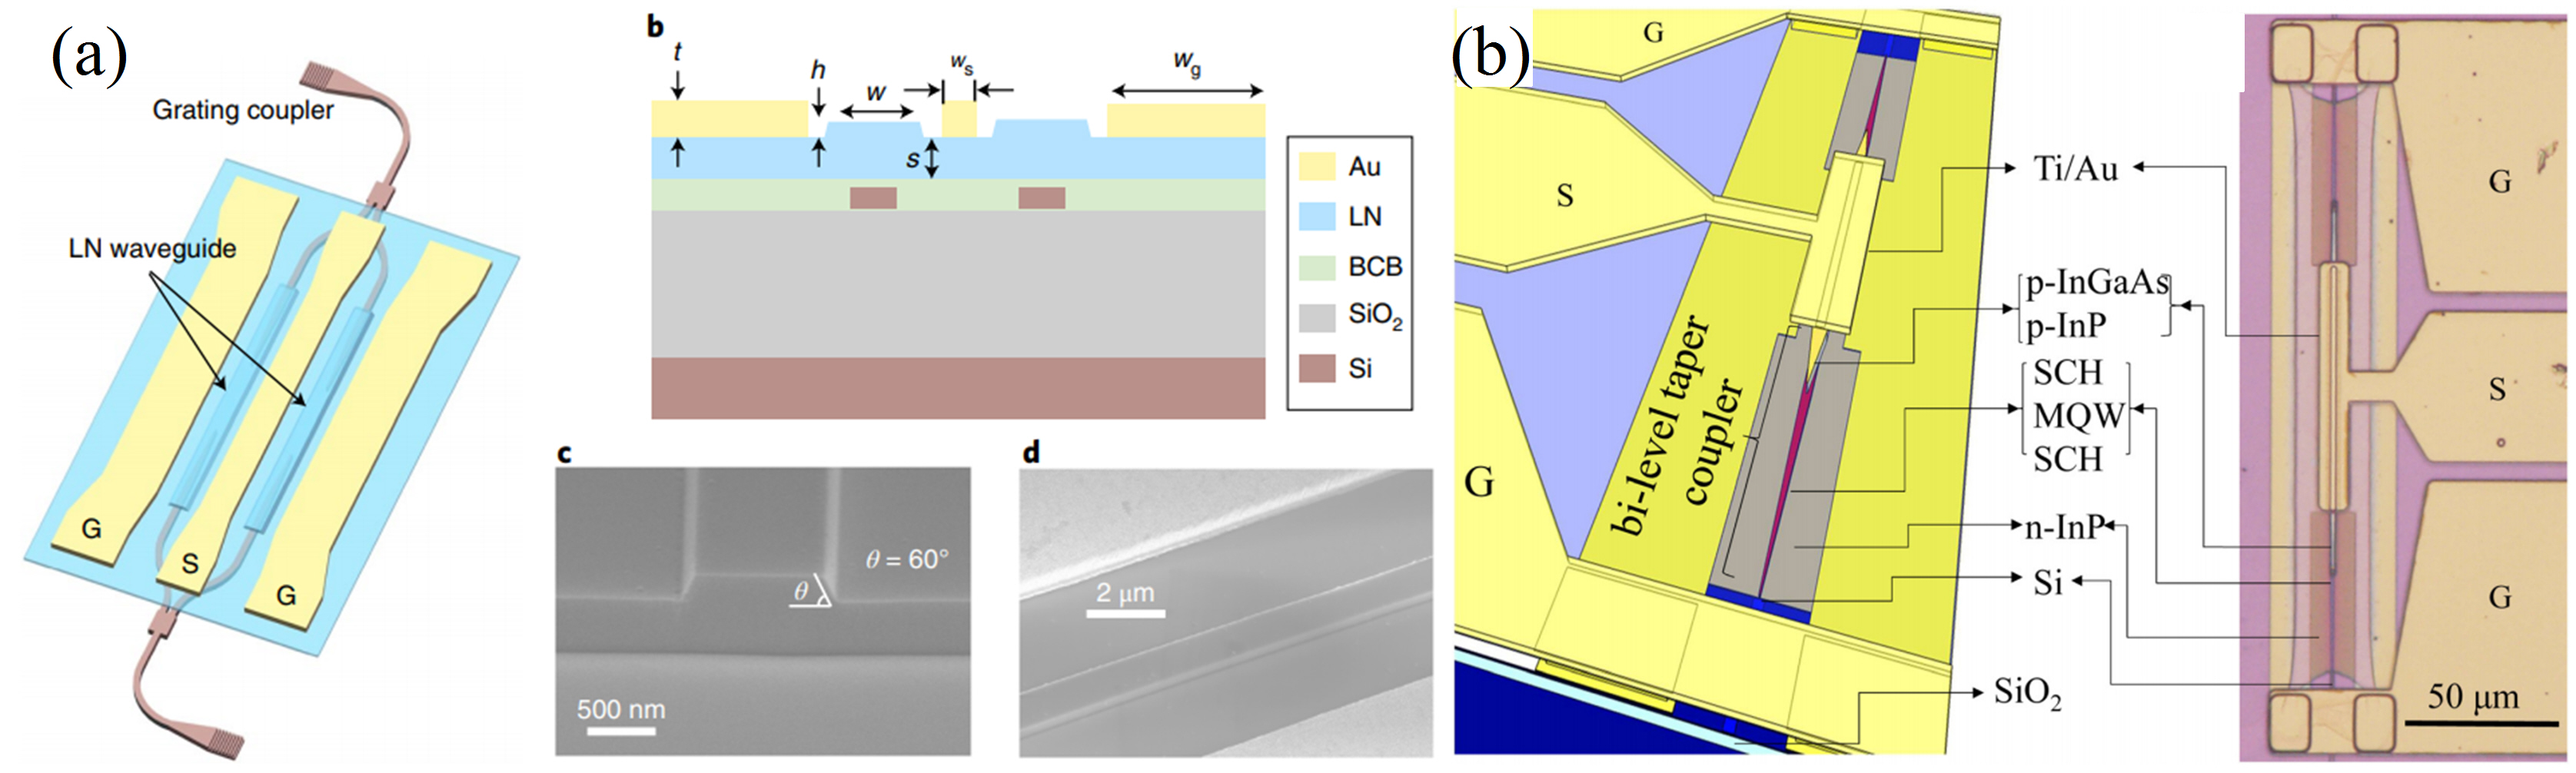
\includegraphics[width=16cm]{./Pictures/intro_external_modulator.jpg}
	\captionsetup{justification=centering}
	\caption{(a)马赫曾德调制器\cite{he2019high}(b)电吸收调制器\cite{huang2016low}}
	\label{intro_external_modulator}
\end{figure}


\subsection{气体检测领域的应用}

随着近几年来,我们对大气污染问题的越来越重视,各种污染物的检测成为政府进行科学合理地制定政策与规划的依据。相比于利用电化学传感器检测易受到干扰的问题,由于不同的气体分子的电子、振动、转动三个能级的不同,其都具有相应的光学吸收谱,故可以利用光学的方法来进行气体的特异性检测,其还具有非接触的特点。

图\ref{intro_ndir}所示为工业上基于NDIR(non-dispersion infrared absorption spectroscopy)的气体传感器示意图,可以实现CO和CO\SB{2}的浓度传感。该传感器从上端发射可以分别被CO和CO\SB{2}吸收的激光,利用CO和CO\SB{2}对不同的波长吸收不同,通过底部探测器得到的光强可以反推出气体的浓度。

\begin{figure}[htb]
	\centering
	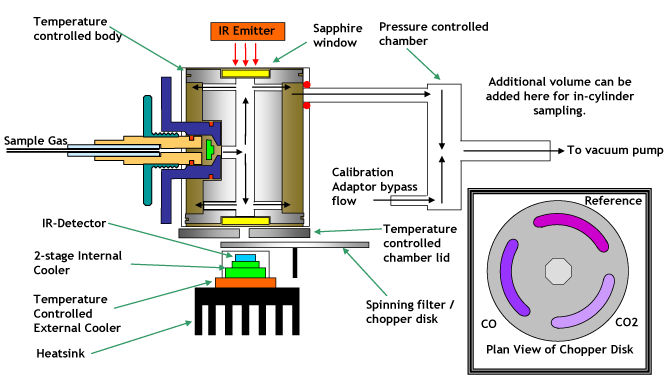
\includegraphics[width=14cm]{./Pictures/intro_ndir.png}
	\captionsetup{justification=centering}
	\caption{工业上基于NDIR的CO与CO\SB{2}传感器\cite{cambustionndir}}
	\label{intro_ndir}
\end{figure}

\section{论文的主要研究工作和创新点}
\subsection{主要内容}

本论文主要的研究工作基于对硅基混合集成自脉冲DFB激光器的研究以及其在三个领域的应用。第一个应用是在微波光子学领域,利用自脉冲DFB激光器的拍频效应,结合探测器可以生成频率可调的微波信号,实验还发现,该微波信号还可以通过注入外调制信号进行频率锁定。第二个应用是在光互联领域,利用光子共振现象,自脉冲DFB激光器可以提升直调带宽,实现更大的数据传输速率。第三个应用是在气体传感领域,利用自脉冲激光器双波长可调的特性,可以将一个激射波长设定到气体的吸收峰上,另一个激射波长位于吸收峰附近作为参考,通过比较,可以进行气体浓度的测量,为此,本文还设计了一个基于EDG的片上高分辨率光谱仪。本文还对在实际加工制作器件的过程中遇到的一些工艺问题做了相应的研究与改进。针对电子束曝光加工大尺寸器件的拼接错位问题,本文提出了一种叫做描边法的加工工艺;针对实验加工过程中刻蚀深度的控制,本文提出了一种根据颜色来判断SOI芯片刻蚀深度的方法,能够方便实验过程中刻蚀深度的确认。

本文的章节安排如下:

第一章为绪论,首先介绍了硅基光电子集成技术的发展背景,接着着重介绍了硅基光电子平台上的光源以及混合集成DFB激光器以及其在气体检测、微波光子学、光互联领域的应用。

第二章首先介绍了硅光集成器件设计中的基本理论和数值仿真方法。本文从麦克斯韦方程组出发,推导了光波导的模式特征方程,简要阐述了光波导模式理论,针对一般情况下波导中光场的传输问题,本文介绍了时域有限差分的数值计算方法。之后,本文介绍了DFB激光器的基本原理。最后,本文介绍了实验室加工制作硅基光子器件的基本方法。

第三章介绍了一种利用SOI芯片颜色来确定硅层厚度的方法,因为在实际器件制作过程中经常需要对SOI芯片做减薄工艺。本章首先介绍了薄硅在硅基光电子器件中的应用及其优势作为例子,然后介绍了光度学和色度学的一些基本内容,利用时域有限差分的数值计算方法,本文给出了不同硅层厚度下SOI芯片的反射谱,根据反射光谱得到了不同硅层厚度对应的颜色,发现当硅层厚度小于120~$nm$之后,随着硅层厚度的变化,颜色变化变得非常明显,这可以帮助实验人员快速确定硅层的厚度。本文将计算结果与实验进行了比较,取得了一致的结果。

第四章首先介绍了自脉冲DFB(distributed feedback laser)激光器及其原理,之后介绍了III-V族材料和硅的混合集成方法。本文设计并制作了一个硅基III-V混合集成的自脉冲DFB激光器,并测试了该自脉冲激光器的性能。产生的自脉冲可以用于微波光子学中光学微波信号的产生并发现了其频率锁定的现象。本文还发现了该自脉冲现象还可以用来提升激光器的调制带宽,并给出了相应的实验结果。

第五章首先结合上一章中自脉冲激光器有双波长的特性,设计了一套由激光器与光谱仪构成的气体浓度检测系统。之后介绍了片上光谱仪的几种实现方案,然后给出了基于EDG的硅基片上高分辨率光谱仪的设计,该光谱仪的输出波导采用密集阵列波导以提升光谱仪的分辨率。本文设计的光谱仪通道数为121,通道间隔为0.5~$nm$。受限于实验室的EBL加工条件,实验上,本文制作了只包含20通道的该EDG光谱仪作为方案的验证,实现了分辨率($\lambda/\Delta\lambda$)高达5571的实验结果,但是其通道间的串扰只有-4.3~dB。本文对实验结果进行了分析,给出了串扰的来源即其解决办法。

第六章对本文主要内容和各项工作进行总结,并展望了未来可以继续优化完善和深入探索的方向。

\subsection{本论文的主要创新点}
本文的创新点主要包括以下几个方面:

\begin{enumerate}[(1)]
	\item 
	本文首次得出了SOI芯片硅层厚度与其显示的颜色之间的关系,得益于硅的高折射率与在可见光波段处的吸收特性,我们可以得到非常丰富的颜色变化信息,尤其当硅层厚度小于120~$nm$时,几纳米的硅层厚度变化,就可以对应非常大的颜色变化,这可以用来快速且较准确地确定硅层的厚度。为了更方便的进行颜色比较,利用人眼对颜色差异的敏感特性,本文还专门开发了一款手机APP用于辅助确定硅层的厚度。根据实验显示,利用该软件,当硅层厚度小于120~$nm$时,可以达到较高的精度。
	\item 
	本文利用III-V族材料和硅的混合集成技术,制作了一个自脉冲DFB激光器。该自脉冲激光器的自脉冲效应可以用于产生光学微波信号,且该微波信号的带宽与激光器的线宽相关联,处于MHz量级。本文发现可以通过外加窄带微波信号,将自脉冲微波信号锁定到特定频率,且其线宽可以小于10~Hz,最小的锁定功率可以达到-17~dBm,为目前报道的最小值。该自脉冲激光器还可以利用光子共振现象提升激光器的调制带宽,本文给出了相应的实验结果,调制带宽可以达到23~GHz,实现了45~Gbps的数据传输速率。
	\item 
	本文提出了一套利用自脉冲激光器的双波长特性与光谱仪结合的气体浓度检测系统。其中一个波长位于气体的吸收峰上,另一个波长位于吸收峰旁作为参考。光谱仪采用基于EDG的设计,首次将密集波导阵列应用到EDG的输出波导中,使其输出波导之间的间距只有1~$\mu m$,提升了EDG光谱仪的分辨率。利用该设计可以在器件尺寸固定时提高光谱仪的分辨率或者在分辨率要求一定时,缩小器件的尺寸。该光谱仪采用双完美成像点的设计方法,包含121个通道,通道间隔0.5~$nm$,覆盖了在1550~$nm$波段60~$nm$的测量范围,并对边缘通道的性能进行了优化,使其通道均匀性更好。实验制作的器件尺寸为3~$mm~\times$~3~$mm$,通道数为20,通道间隔为0.5~$nm$,分辨率($\lambda/\Delta\lambda$)达到5571,是目前已知的基于片上EDG的光谱仪的最高值,且该EDG光谱仪具有集成121通道的潜力,这是其他设计方法较难实现的。
	\end{enumerate}



\chapter{光波导与DFB激光器的基本理论}
\section{光波导理论分析}
在集成光学中,通常使用平面介质光波导来控制光波的传输,即负责光波从器件中的导入与导出,类似于电路中的导线。在很多应用中,波导又是光电子器件中重要的组成部分。可以这样说,平面光波导理论是集成光学的基础理论之一。结构最简单的平面光波导是由三层均匀介质组成的平板波导,如图\ref{fab_slab_waveguide}所示:

\begin{figure}[htb]
	\centering
	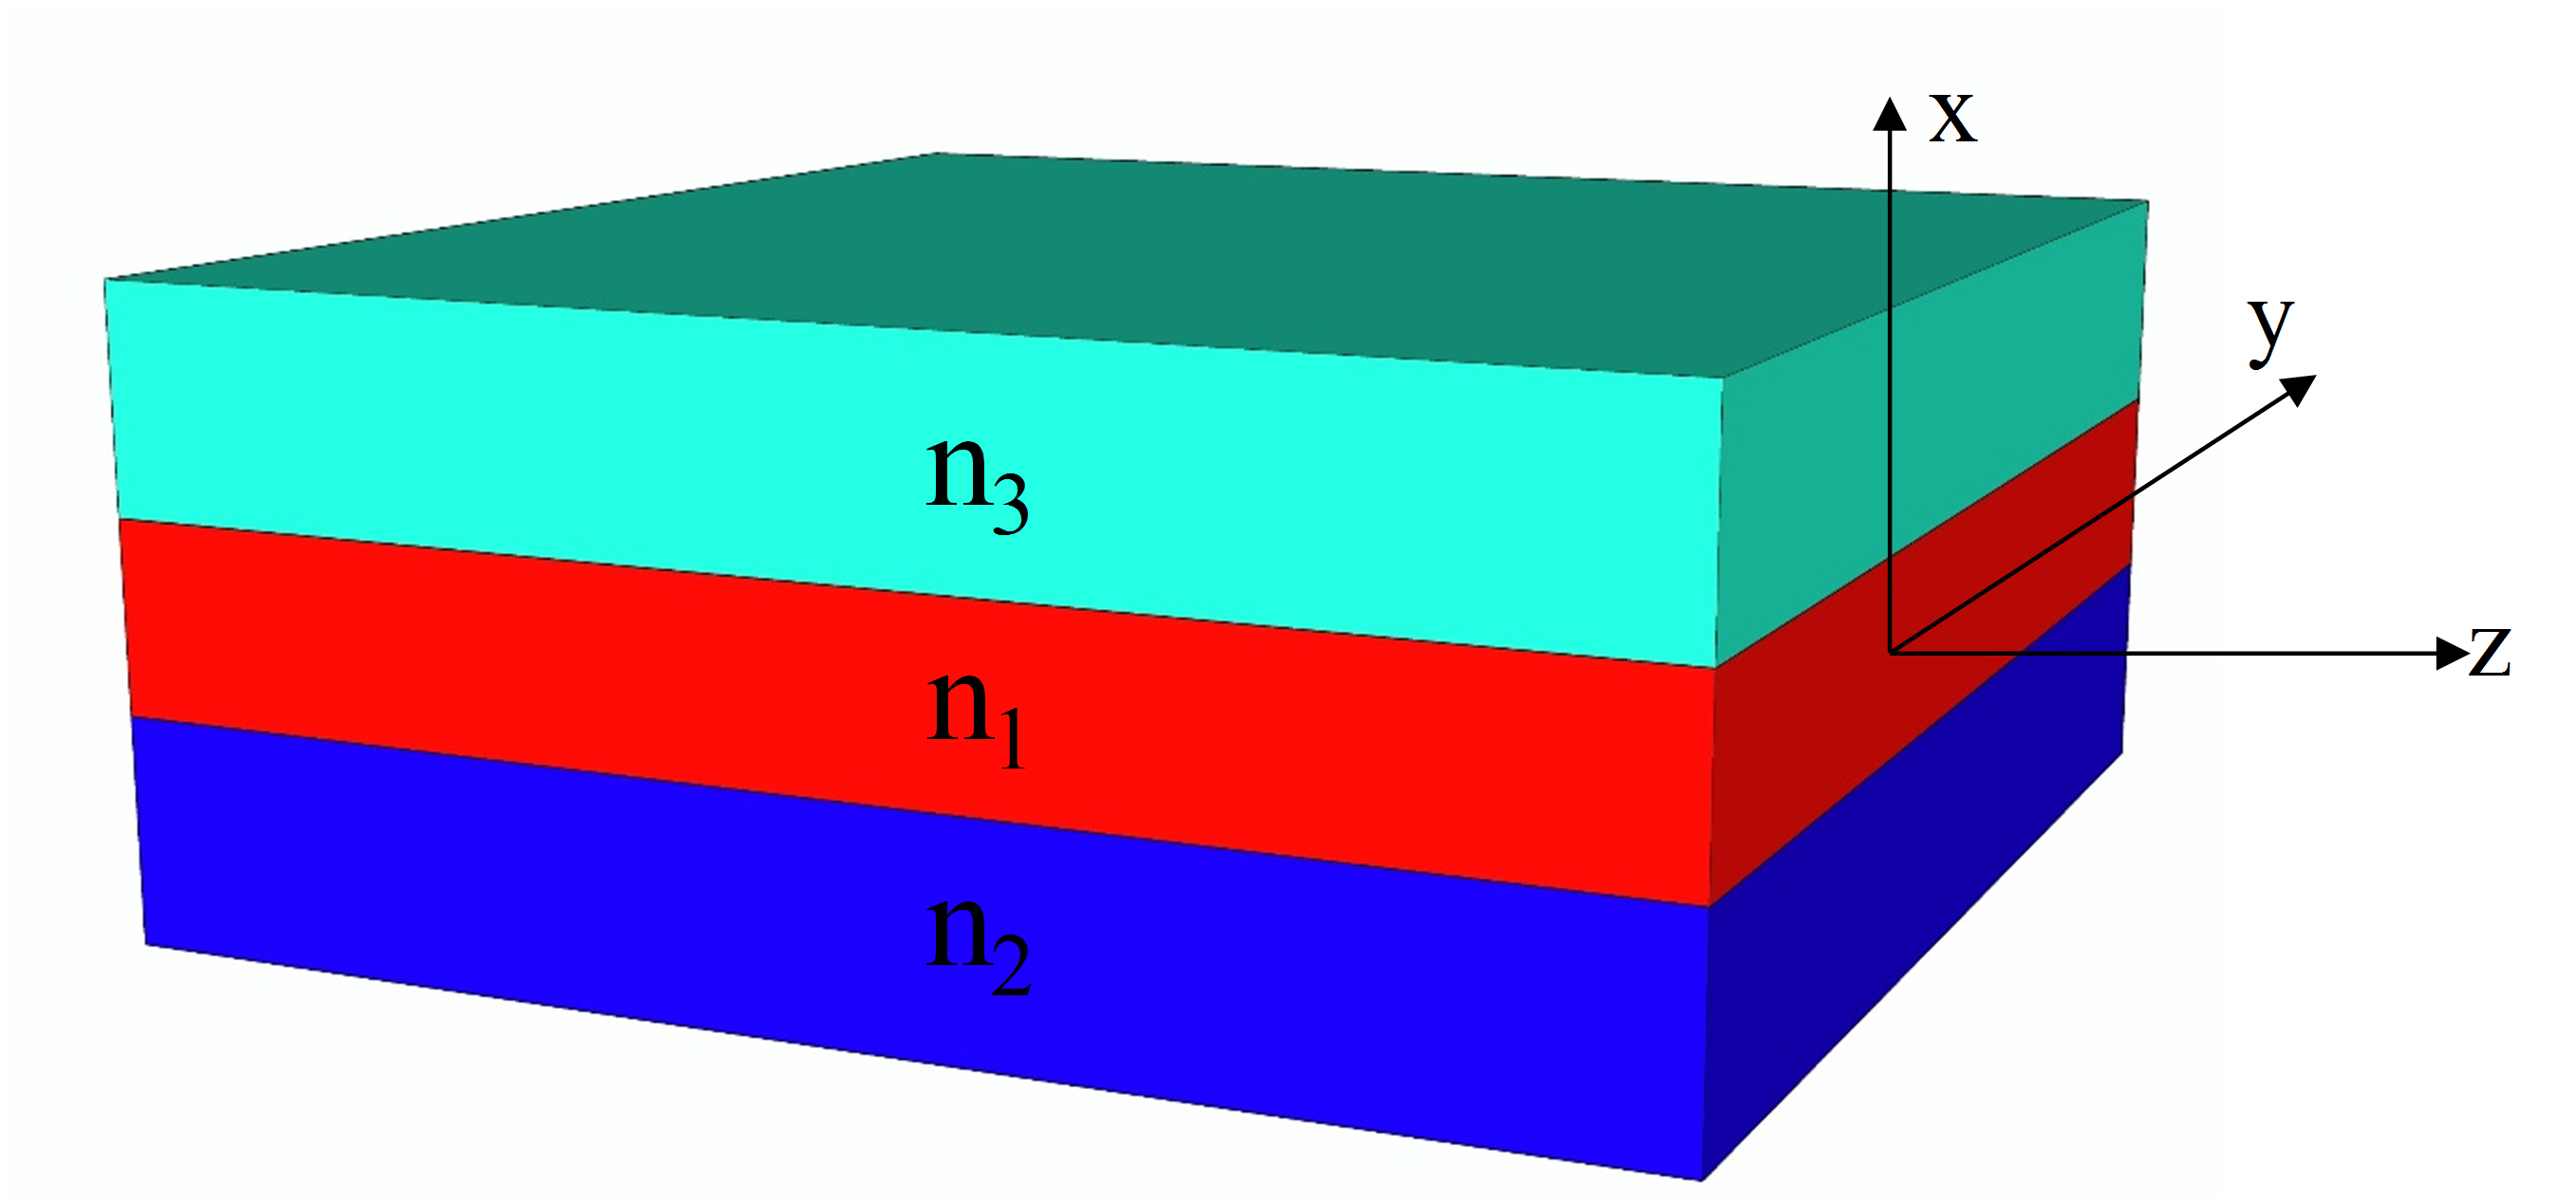
\includegraphics[width=12cm]{./Pictures/fab_slab_waveguide.jpg}
	\captionsetup{justification=centering}
	\caption{三层平板波导结构示意图}
	\label{fab_slab_waveguide}
\end{figure}

其中,为了保证光在波导中稳定传播,必须满足条件$n_{1}>max(n_{2},n_{3})$。该结构中间介质的折射率$n_{1}$最大,称为芯层;两侧介质的折射率较小,称为包层,理解平板波导的传输模式一般有射线光学和波动光学两种方式。射线光学方法对平板波导的模式传输解释通俗易懂,也能获得一些有价值的结论。但是当波导结构变复杂,比如条形波导、脊型波导,射线光学方法就无能为力了,为了对复杂波导的场分布、传输功率等问题进行分析,必须使用波动光学的方法,应用电磁场理论求解电磁波在介质波导这样一种特殊边界条件下的波动方程解,在此基础上再去分析传播模式的特性。

\subsection{波动方程}

要使用电磁场理论就不得不介绍麦克斯韦方程组,麦克斯韦在前人的电磁学研究成果基础上,总结推广了恒定和似穏电磁场的基本规律,提出了时变电磁场的传播规律,将它归纳为一组表达式,称之为麦克斯韦方程组。麦克斯韦方程组有微分和积分两种形式,微分形式的麦克斯韦方程组可以用来求解电磁场中某一处的场量,其表达式如公式\ref{maxwell1}~\~{}~\ref{maxwell4}所示:
\begin{equation}
\label{maxwell1}
\nabla \times \textbf{E} = -\dfrac{\partial\textbf{B}}{\partial t}
\end{equation}

\begin{equation}
\label{maxwell2}
\nabla \times \textbf{H} = \dfrac{\partial\textbf{D}}{\partial t}+\textbf{J}
\end{equation}

\begin{equation}
\label{maxwell3}
\nabla \cdot \textbf{D} = \rho
\end{equation}

\begin{equation}
\label{maxwell4}
\nabla \cdot \textbf{B} = 0
\end{equation}

式中,\textbf{D}、\textbf{E}、\textbf{B}、\textbf{H}分别表示电感强度(电位移矢量)、电场强度、磁感强度和磁场强度;$\rho$表示电荷密度;\textbf{J}表示传导电流密度;$\dfrac{\partial\textbf{D}}{\partial t}$表示位移电流密度,$\nabla$表示nabla算符,它既是微分算符,又是矢量。

在处理实际问题时,电磁场总是在媒质中传播的,所以我们需要物质方程来描述媒质对电磁场传播的影响。在静止的、各向同性媒质中,物质方程如下:

\begin{equation}
\label{constitutive_relations}
\left\{
\begin{array}{c}
\textbf{J}=\sigma\textbf{E}\\
\textbf{D}=\epsilon\textbf{E}\\
\textbf{B}=\mu\textbf{H}
\end{array}
\right.
\end{equation}
式中,$\sigma$是电导率,我们考虑介质波导的时候,$\rho=0$,$\sigma=0$;$\epsilon$是介电常数,在真空中$\epsilon=\epsilon_{0}=8.8542\times10^{-12}C^{2}/N\cdot m^{2}$,在介质中,$\epsilon=\epsilon_{0}\epsilon_{r}$,$\epsilon_{r}$为相对介电常数;$\mu$是磁导率,对于非磁性物质,$\mu_{r}=1$,$\mu=\mu_{0}\mu_{r}=4\pi\times10^{-7}N\cdot s^{2}/C^{2}$。

分别对公式\ref{maxwell1}和公式\ref{maxwell2}取旋度,利用公式\ref{constitutive_relations},并且令$v=1/\sqrt{\epsilon\mu}$,则\textbf{E}、\textbf{H}的方程化为:

\begin{equation}
\nabla^{2}\textbf{E}-\dfrac{1}{v^{2}}\dfrac{\partial^{2}\textbf{E}}{\partial t^{2}}=0
\end{equation}
\begin{equation}
\nabla^{2}\textbf{H}-\dfrac{1}{v^{2}}\dfrac{\partial^{2}\textbf{H}}{\partial t^{2}}=0
\end{equation}

考虑时谐电磁场,即$\textbf{E}=\textbf{E}_{0}e^{-i\omega t}$,$\textbf{H}=\textbf{H}_{0}e^{-i\omega t}$可以得到时谐波动方程,即本征频率问题:
\begin{equation}
\label{helmholtz1}
\nabla^{2}\textbf{E}+k^{2}\textbf{E}=0
\end{equation}
\begin{equation}
\label{helmholtz2}
\nabla^{2}\textbf{H}+k^{2}\textbf{H}=0
\end{equation}
其中,$k=k_{0}n=\omega \sqrt{\mu_{0}\epsilon}$,$k_{0}=\dfrac{2\pi}{\lambda_{0}}$为真空中的波矢,$\omega$为光波角频率,n是材料的折射率,c是真空中的光速,公式\ref{helmholtz1}~\~{}~\ref{helmholtz2}也被叫亥姆霍兹方程。

假设电磁场沿z轴方向传播时,沿z方向电磁场的变化可以用传输因子$e^{-j\beta z}$来表示,其中$\beta=k_{0}n_{eff}$为传播常数,$n_{eff}$为模式的等效折射率,即电磁场可以写成如下形式:
\begin{equation}
\label{betaz1}
\textbf{E}=\textbf{E}(x,y)e^{-i\beta z}
\end{equation}
\begin{equation}
\label{betaz2}
\textbf{H}=\textbf{H}(x,y)e^{-i\beta z}
\end{equation}

将公式\ref{betaz1}、\ref{betaz2}分别带入公式\ref{helmholtz1}、\ref{helmholtz2},则$\dfrac{\partial}{\partial z}$可以用$-j\beta$代替,$\dfrac{\partial^{2}}{\partial z^2}$可以用$-\beta^2$代替,从而可以得到直角坐标系下的矢量波动方程:
\begin{equation}
\label{helmholtz3}
\left(\dfrac{\partial^2}{\partial x^2}+\dfrac{\partial^2}{\partial y^2}\right)\textbf{E}(x,y)+(k_0^2n^2-\beta^2)\textbf{E}(x,y)=0
\end{equation}
\begin{equation}
\label{helmholtz4}
\left(\dfrac{\partial^2}{\partial x^2}+\dfrac{\partial^2}{\partial y^2}\right)\textbf{H}(x,y)+(k_0^2n^2-\beta^2)\textbf{H}(x,y)=0
\end{equation}

在实际求解过程中,光有亥姆霍兹方程的解会有无穷多组,还要考虑边界条件得到具有实际物理意义的解。利用波动方程\ref{helmholtz3}、\ref{helmholtz4}以及边界条件,可以得到一系列波导的本征模式解,它们具有如下特性:
\begin{enumerate}[(1)]
	\item 
	色散性~~~~不同的本征模式有不同的等效折射率$n_{eff}$,其各自沿传播方向有一个等效的传播相速度$v_{eff}=c/n_{eff}$
	\item 
	正交性~~~~不同本征模式间的场分布叠加积分为零,意味着在沿传播方向均匀的波导中,本征模式之间不存在串扰。
	\item 
	完备性~~~~任意能在介质波导中稳定传输的光场都可以分解为本征模式的线性叠加,光场的传播特性由这些本征模式的特性所决定。
\end{enumerate}

综上,我们可以通过研究波导各本征模的特性,就可以知道任意稳定传输光场的传播特性。故对本征模式模场分布和等效折射率的求解计算便成了设计、分析波导结构的基础与关键。

\section{光波导的数值计算方法}

对于如图\ref{fab_slab_waveguide}所示的平板波导,可以利用解析的方法得到其本征模式的特征方程\cite{ttt2005jcgx}。但是当电磁场在平板波导中传输时,在无约束的方向上会发散,这不利于器件的集成,为了避免这种情况,集成光学中常使用的三维波导结构如图\ref{fab_strip_waveguide}所示:

\begin{figure}[htb]
	\centering
	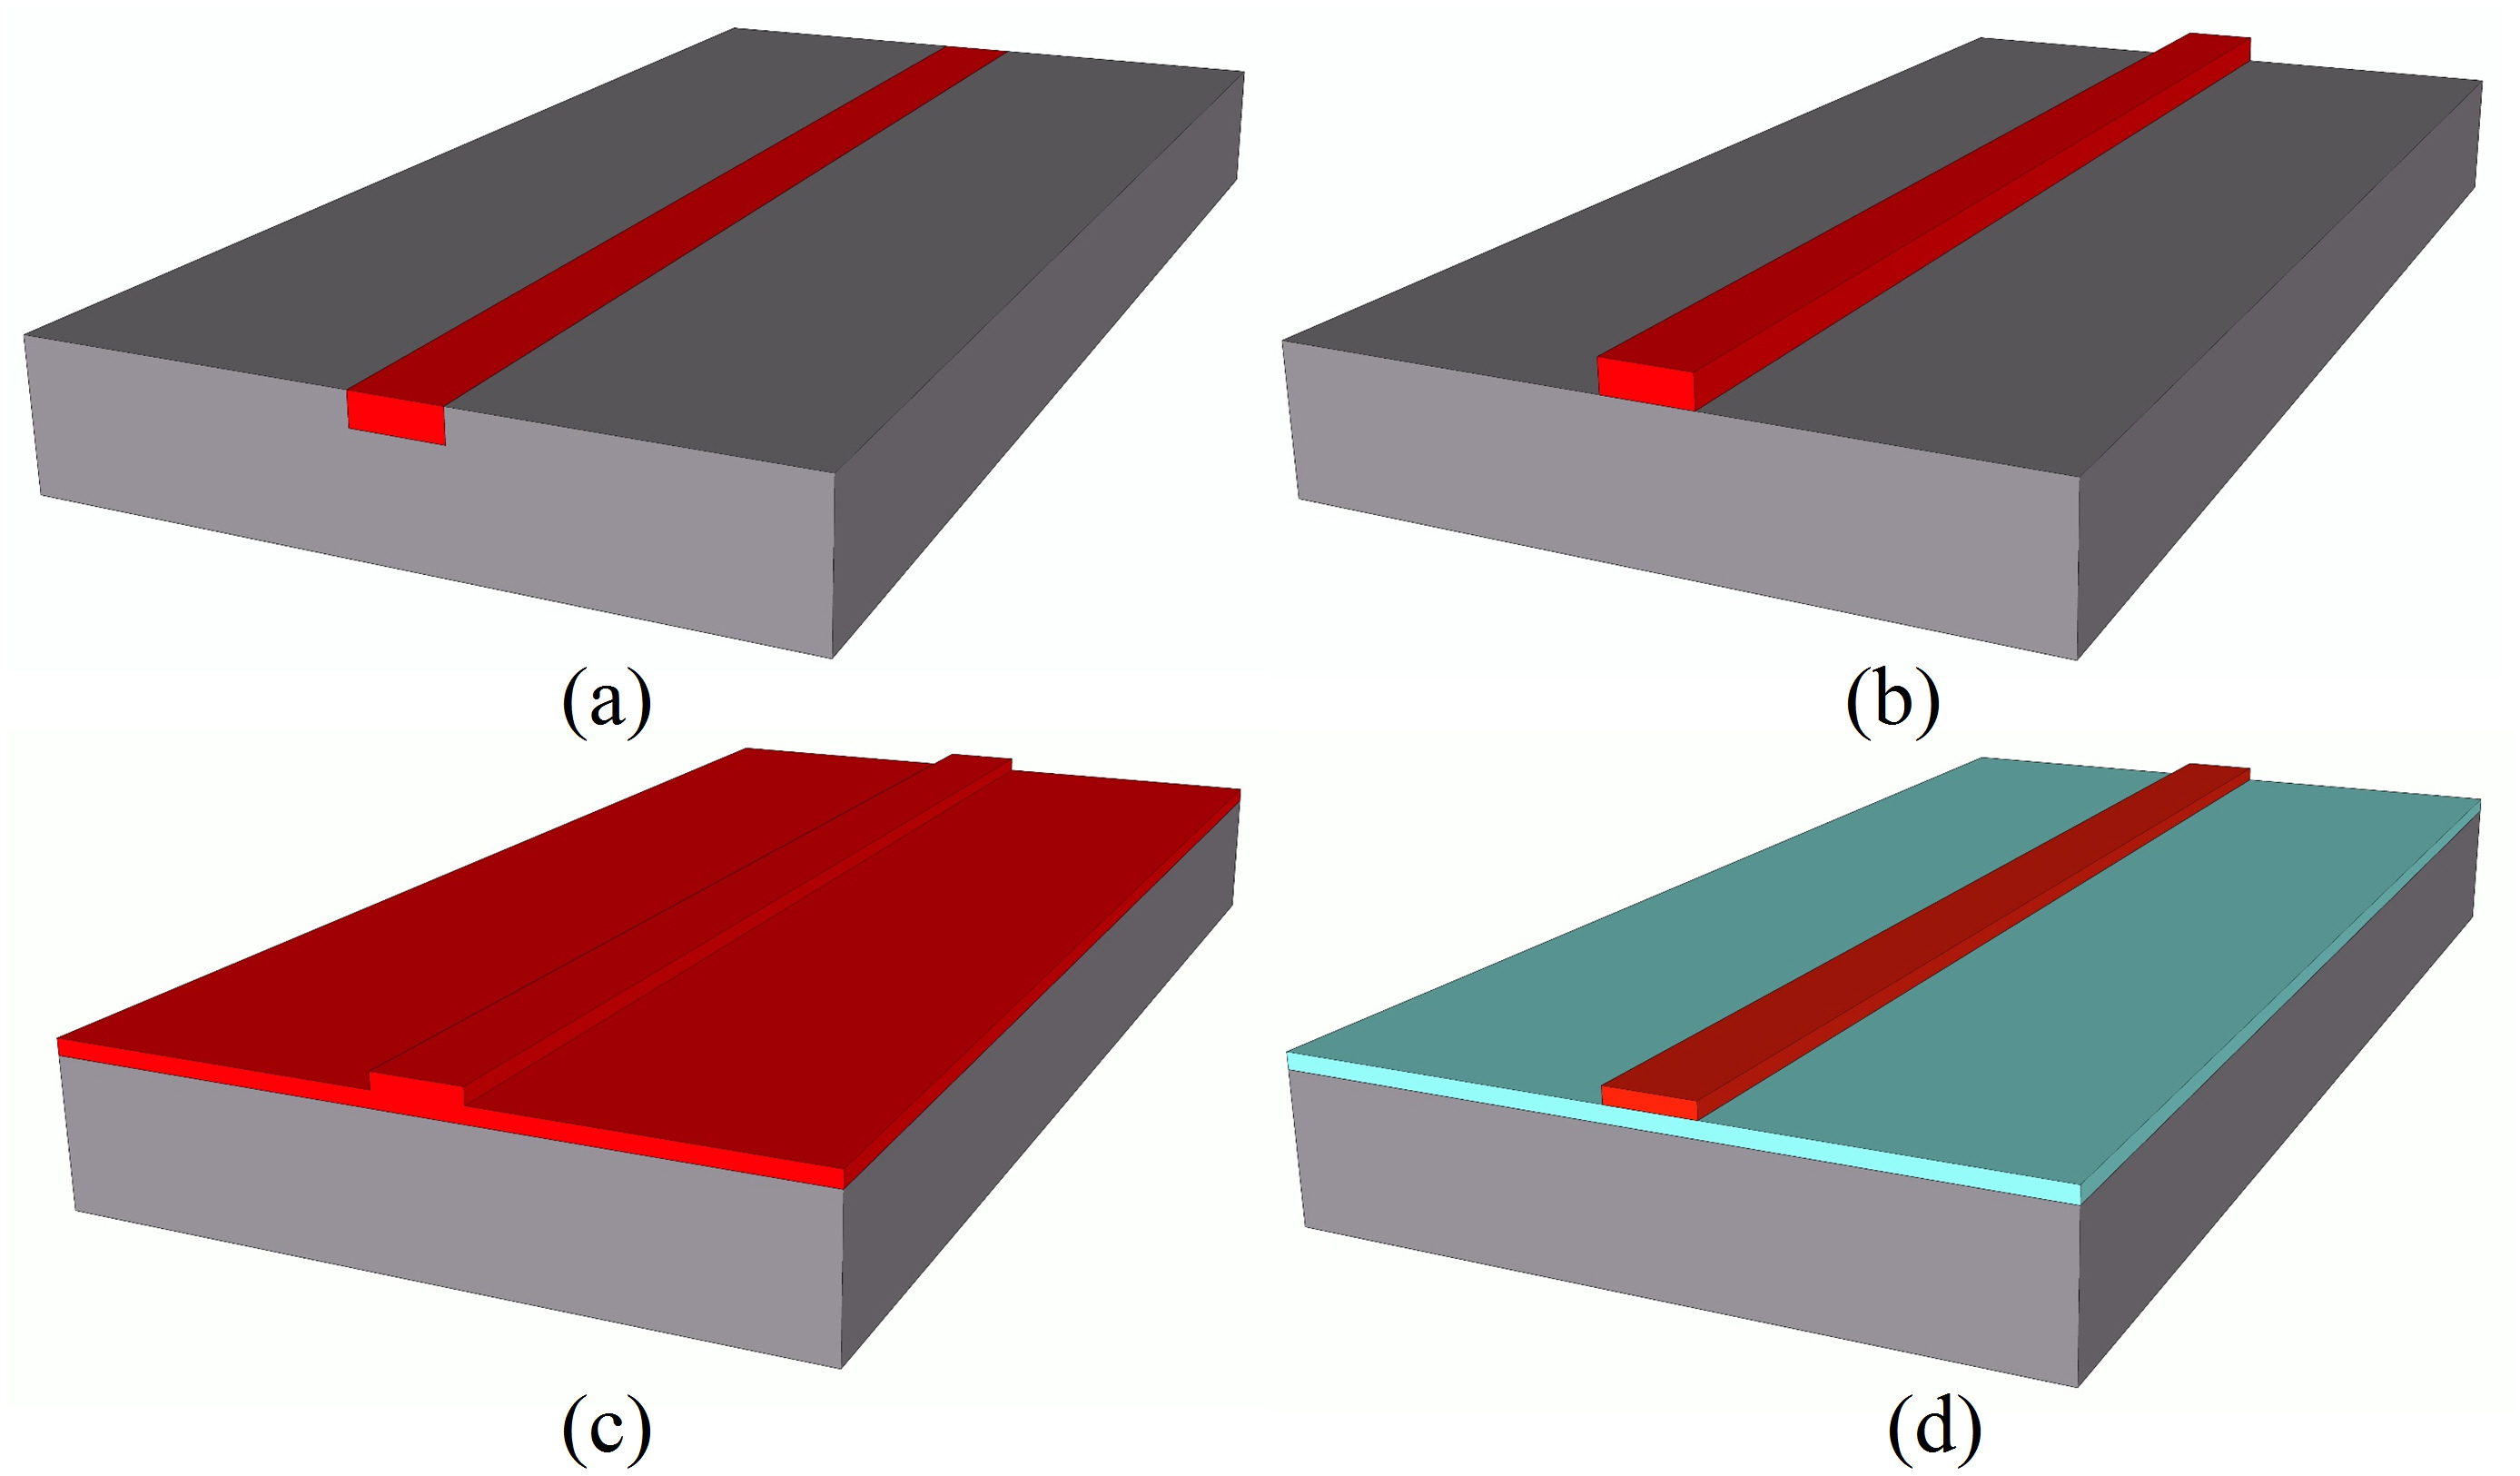
\includegraphics[width=13cm]{./Pictures/fab_strip_waveguide.jpg}
	\captionsetup{justification=centering}
	\caption{几种常见的光波导结构:(a)掩埋型;(b)条带型;(c)脊型;(d)条载型}
	\label{fab_strip_waveguide}
\end{figure}

三维波导与二维平板波导不同,没有严格的解析模式解,只能用近似分析法或者数值方法求解。在弱导近似下,主要模式光能基本被限制在芯层波导中传输,这时三维波导中存在的不再是TE模式或者TM模式,而存在以$E_y$、$H_x$为主的$E_{mn}^y$模式(或称为似TE模)和以$H_y$、$E_x$为主的$E_{mn}^x$模式(或称为似TM模)。模式的上标x、y表示电场矢量的偏振方向(坐标系与图\ref{fab_slab_waveguide}一样),下标m、n为模式序号,代表场量在x轴和y轴方向出现场量最大值的个数。与平板波导波导相比,条形波导的分析要复杂的多,通常使用的近似分析法有Marcatili方法和等效折射率法\cite{okamoto2006fundamentals}。但是得益于现在计算机计算能力的提升,我们很少需要用到这两种方法去近似求解亥姆霍兹方程,采用的往往是用数值方法进行模拟计算,只要数值离散足够精细,就能获得非常精确的结果。常见的本征模式数值求解法主要有有限差分法(finite difference method, FDM)\cite{stern1988semivectorial}和有限元法(finite element method, FEM)\cite{jin2015finite}两种。该两种方法的核心思想都是将连续问题离散化,进而转化为有限形式的线性方程组进行数值求解,其过程大致可以分为以下两步:1、对求解区域进行网格划分,其中FDM采用的是矩形网格,而FEM一般采用三角形的网格。2、用差分方程代替微分算子,将偏微分方程的求解问题转化为有限个线性代数方程组的求解问题。相对于FEM,FDM方法容易理解、效率较高,但是FEM由于网格划分比较灵活,具有更好的适应性和精度。商用软件Lumerical Mode Solutions\cite{modesolution}采用FDM,COMSOL\cite{comsol}则采用FEM。

\subsection{时域有限差分法}

在实际的平面集成光器件的设计过程中,计算出模式的分布往往还不够,我们需要计算光场的传输,常用的方法有光束传播方法(beam~propagation~method,~BPM)\cite{van1981beam},本征模式展开法(eigenmode~expansion,~EME)\cite{gallagher2003eigenmode},时域有限差分法(finite~difference~time~domain,~FDTD)\cite{yee1966numerical}。光束传播方法(BPM)由于采用了标量近似和傍轴近似,因此无法获得模式的偏振和反射信息且只能仿真光场沿光轴缓慢变化的情况,这对于基于SOI的集成光学器件仿真是不适用的。本征模展开法(EME)虽然是一种全矢量、双向的算法,且能够计算大角度的光场传输,但是其是在频域求解麦克斯韦方程组,故其每次只能进行单频率点的仿真。时域有限差分法(FDTD)是一种能够精确求解任意结构中麦克斯韦方程组的算法,其直接对麦克斯韦方程组进行离散化,仿真区域被离散成一个个Yee元胞,除了将连续的物理空间用离散的空间格点所引入的近似以外,没有引入其他任何的近似。由于FDTD是基于时域的算法,其经过一次仿真,经过傅里叶变换之后就可以得到一段频谱范围内的响应。FDTD是1966年的时候由Yee博士首次提出的,随后经过很多人的改进,如今已经被广泛应用到诸如太阳能电池的设计、CMOS图像传感器设计、超材料设计、集成光电子器件设计等电磁学的各个领域。

\begin{figure}[htb]
	\centering
	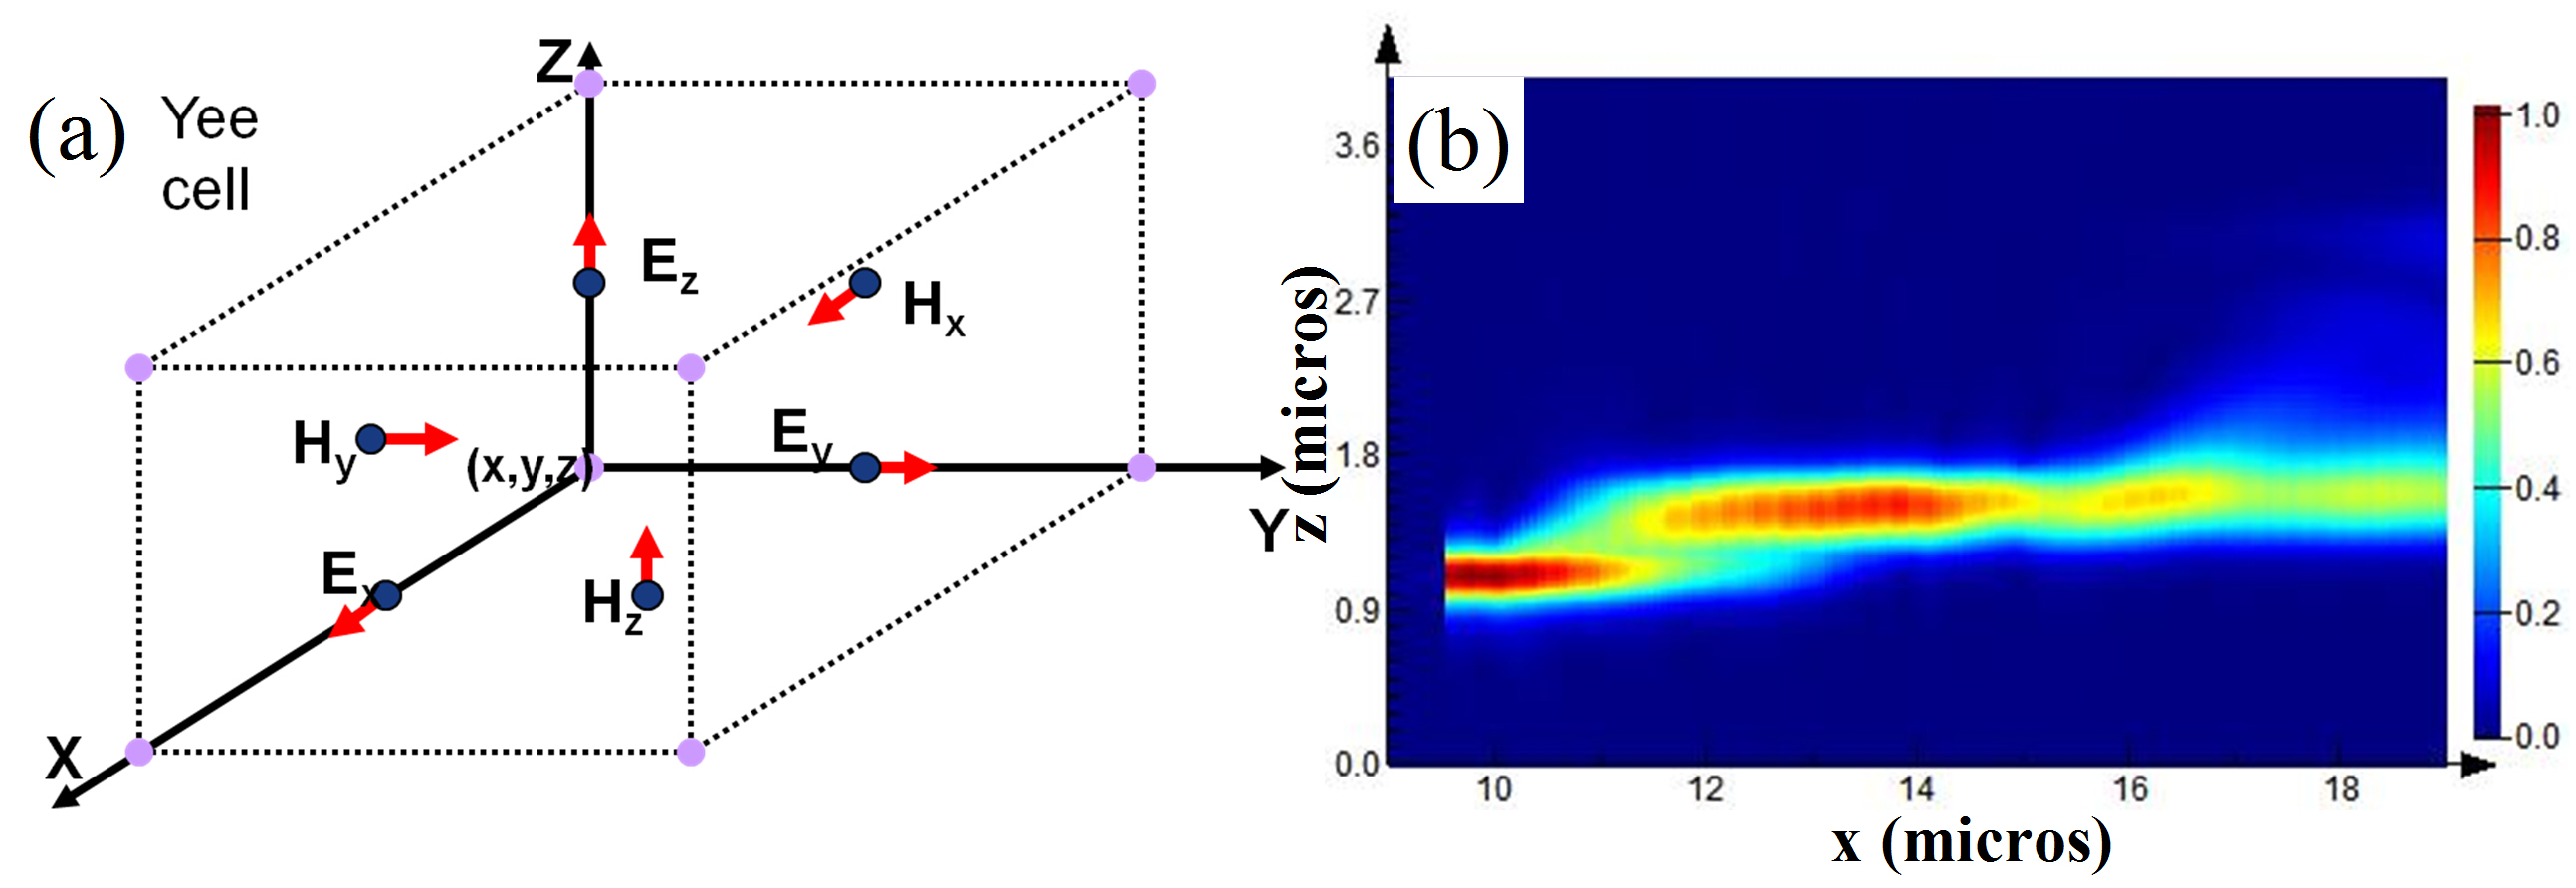
\includegraphics[width=16cm]{./Pictures/fab_yeecell.jpg}
	\captionsetup{justification=centering}
	\caption{(a)三维直角坐标系下的Yee网格的分布图\cite{fdtdsolution};(b)~FDTD算法计算得到的光场传输图}
	\label{fab_yeecell}
\end{figure}

图\ref{fab_yeecell}(a)所示为直角坐标系下的Yee网格示意图,其中电场分量位于网格单元每条棱的中心点处,磁场分量位于网格单元的每个面中心,这种电、磁场分量交叉分离划分的方法能够确保它们各自的分量在介质分界面处连续,而且利用这种网格划分方法,不但可以实现方程在三维空间中的差分运算,而且也同时满足了安培环路积分定律和法拉第电磁感应定律。因此利用该种网格划分方法对空间进行离散化,可以准确地被用来模拟电磁场在介质波导中的实际传输过程。图\ref{fab_yeecell}(b)为本文利用FDTD计算垂直耦合结构的耦合效率时得到的光场传输图。

\section{DFB激光器的基本原理}

激光器产生激射的三个条件分别是:1增益介质,2谐振腔,3泵浦源。谐振腔通过把一部分光周期性地反射回原来的地方,对于某些波长来说刚好满足干涉增强的条件,并通过被泵浦的增益介质实现受激放大,从而产生激光\cite{numai2015fundamentals,suhara2004semiconductor}。

对于半导体激光器来说,当导带中的电子与价带中的空穴复合时,就会产生光子。该过程中需要满足能量守恒与动量守恒。能量守恒决定了出射光子的能量,其等于电子与空穴所处能级的能量差。动量守恒决定了只有直接带隙半导体才能比较高效地发光。常用的直接带隙材料包括AlGaAs,InGaAs和InGaAsP,其带隙可以通过改变不同元素的组分进行调节,从而可以控制激光器的激射波长。

对于最简单的FP(Fabry-Perot)激光器来说,谐振腔由两个解理的端面组成,FP激光器的优点是结构简单,但由于材料的增益谱往往比较宽,会覆盖多个FP腔的纵模,故其出射为多纵模,使得其不适用于光通信系统,因为多个波长的存在会加剧光纤的色散影响。如图\ref{fab_fp_laser}所示FP激光器激射模式示意图,每个纵模的波长满足谐振条件:
\begin{equation}
m\lambda = 2n_e(\lambda)L
\end{equation}
其中$L$为激光器的腔长,$n_e(\lambda)$为等效折射率。

\begin{figure}[htb]
	\centering
	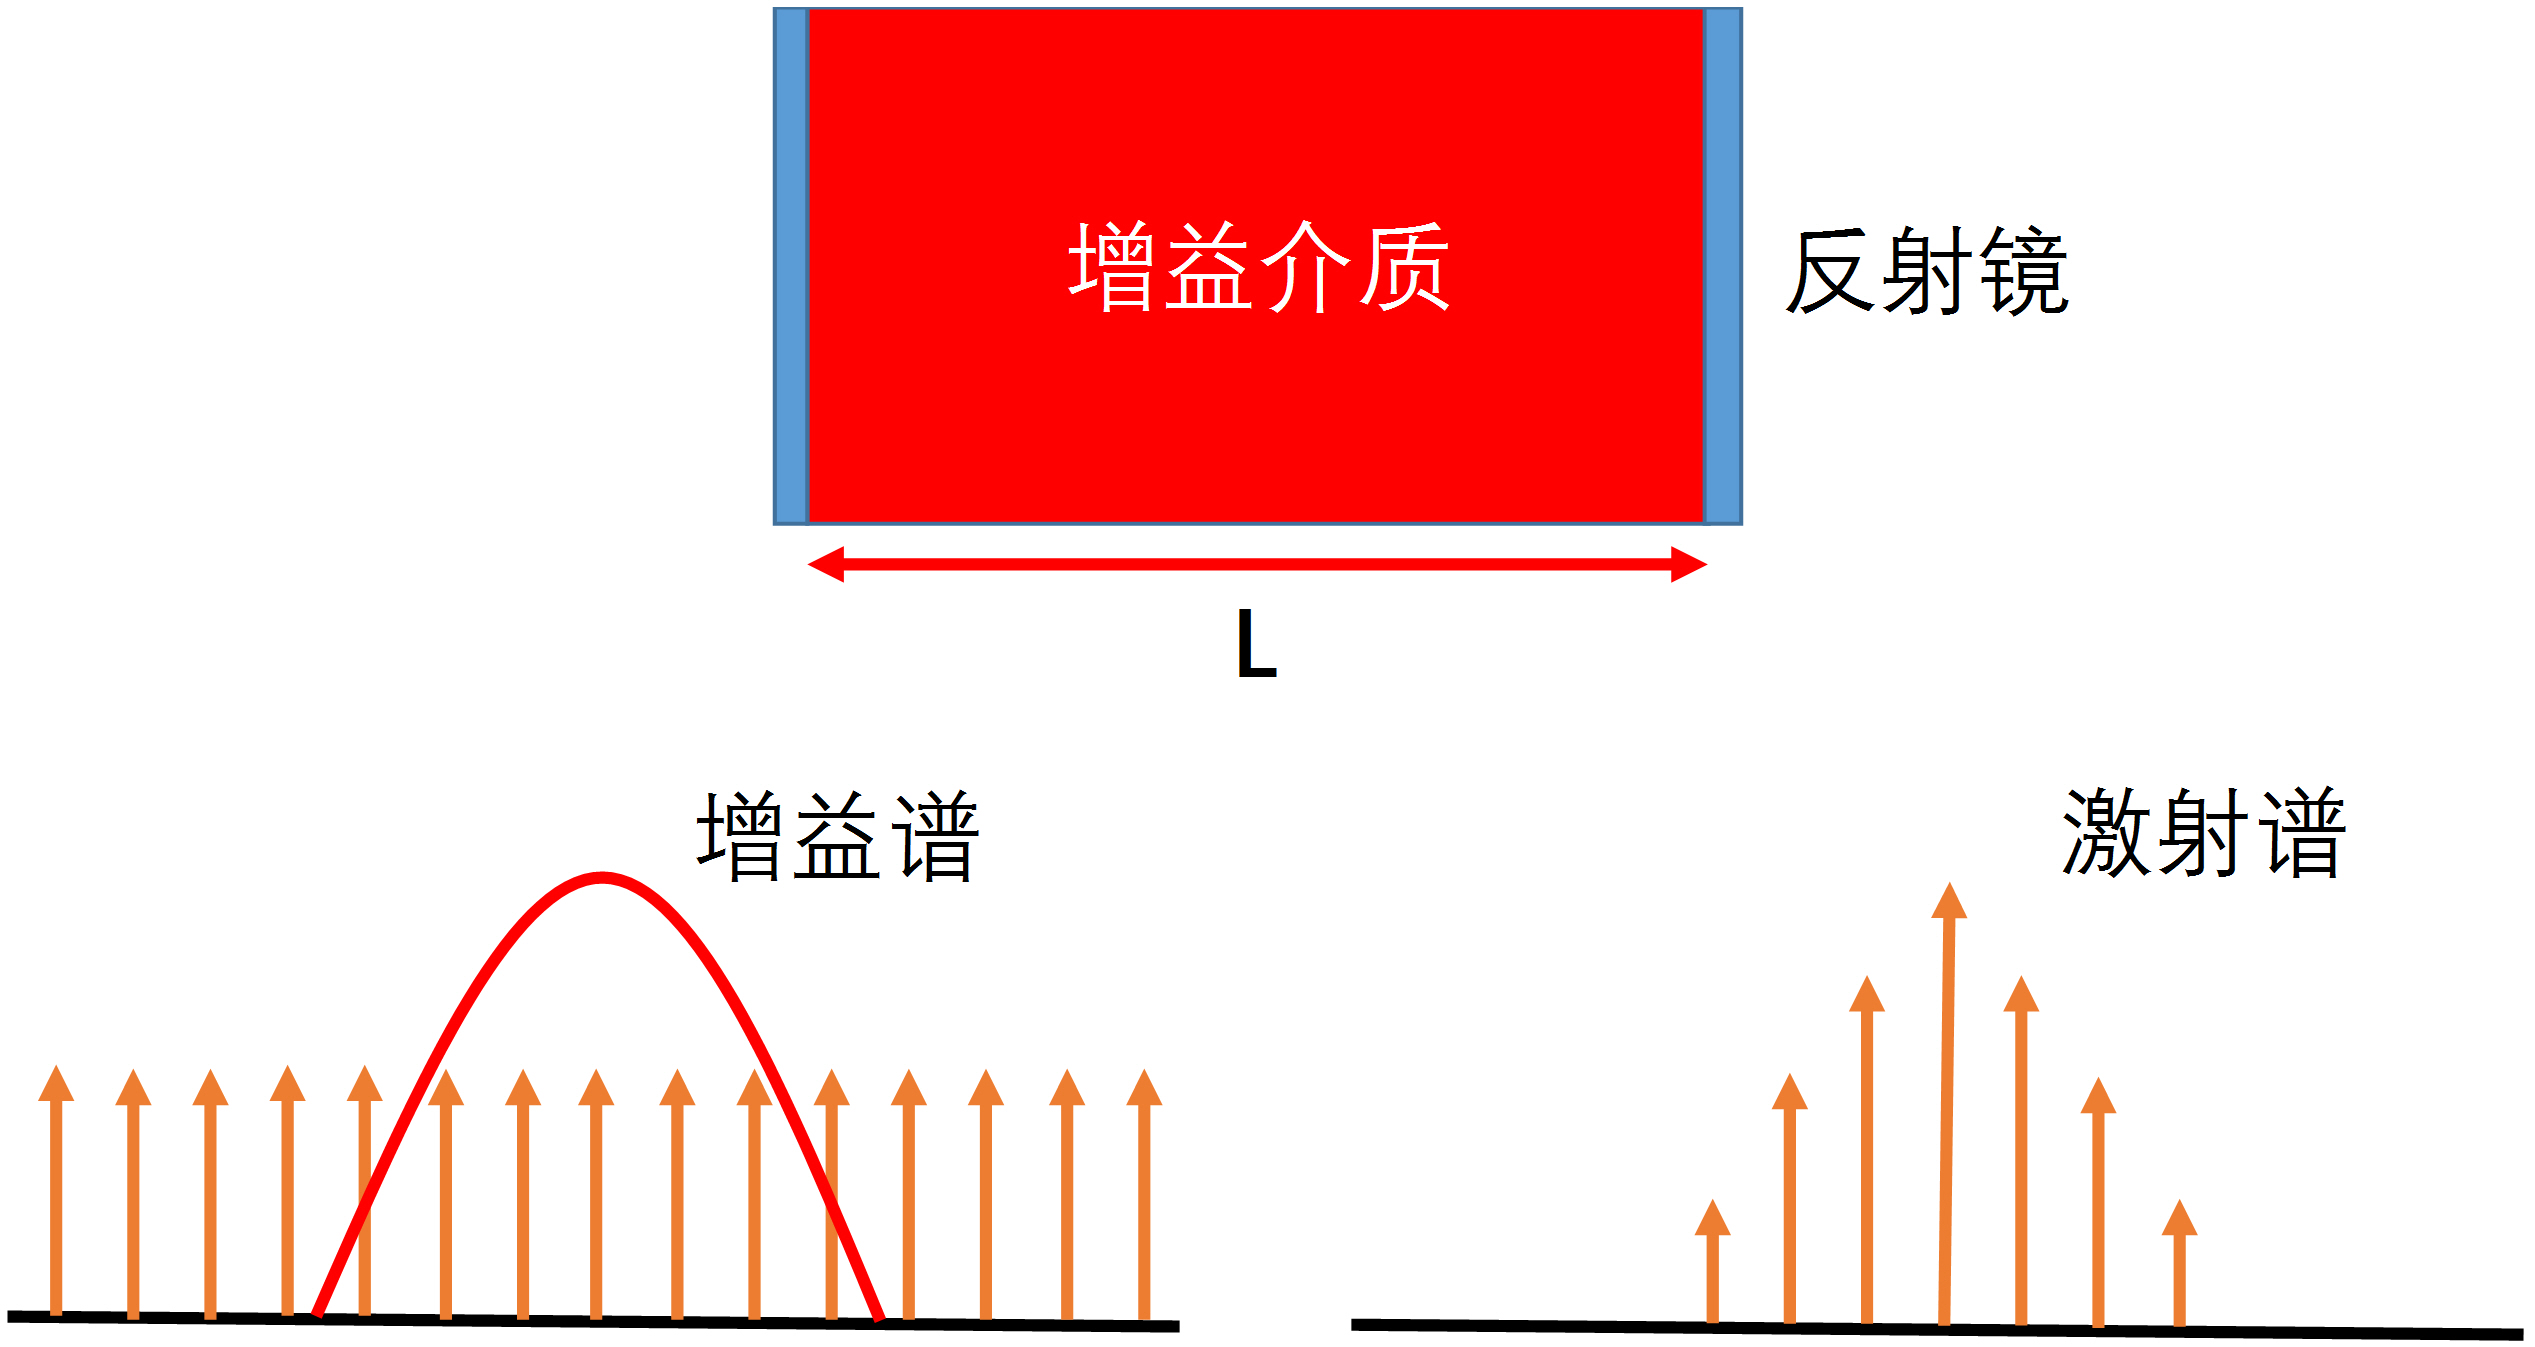
\includegraphics[width=12cm]{./Pictures/fab_fp_laser.jpg}
	\captionsetup{justification=centering}
	\caption{FP激光器激射模式示意图}
	\label{fab_fp_laser}
\end{figure}

DFB激光器通过将FP激光器中由两面反射镜构成的简单谐振腔替换成分布反馈布拉格反射镜,可以克服FP激光器的多模问题,只出射一个纵模,其激射模式示意图如图\ref{fab_dfb_laser}所示。分布反馈布拉格光栅可以通过周期性地改变波导的宽度或者厚度来实现,从而周期性地改变波导的等效折射率。当光经过布拉格光栅时,在每个折射率突变的界面都会产生反射,使得前向传输的光与背向传输的光相互耦合。由于分布反馈布拉格光栅的周期往往只有几百纳米,故其产生的自由频谱范围(free spectral range, FSR)较大,可以在增益介质的增益带宽内实现单纵模激射。对于DFB激光器来说,可以通过改变分布反馈布拉格光栅的周期和等效折射率来改变激射波长。

\begin{figure}[htb]
	\centering
	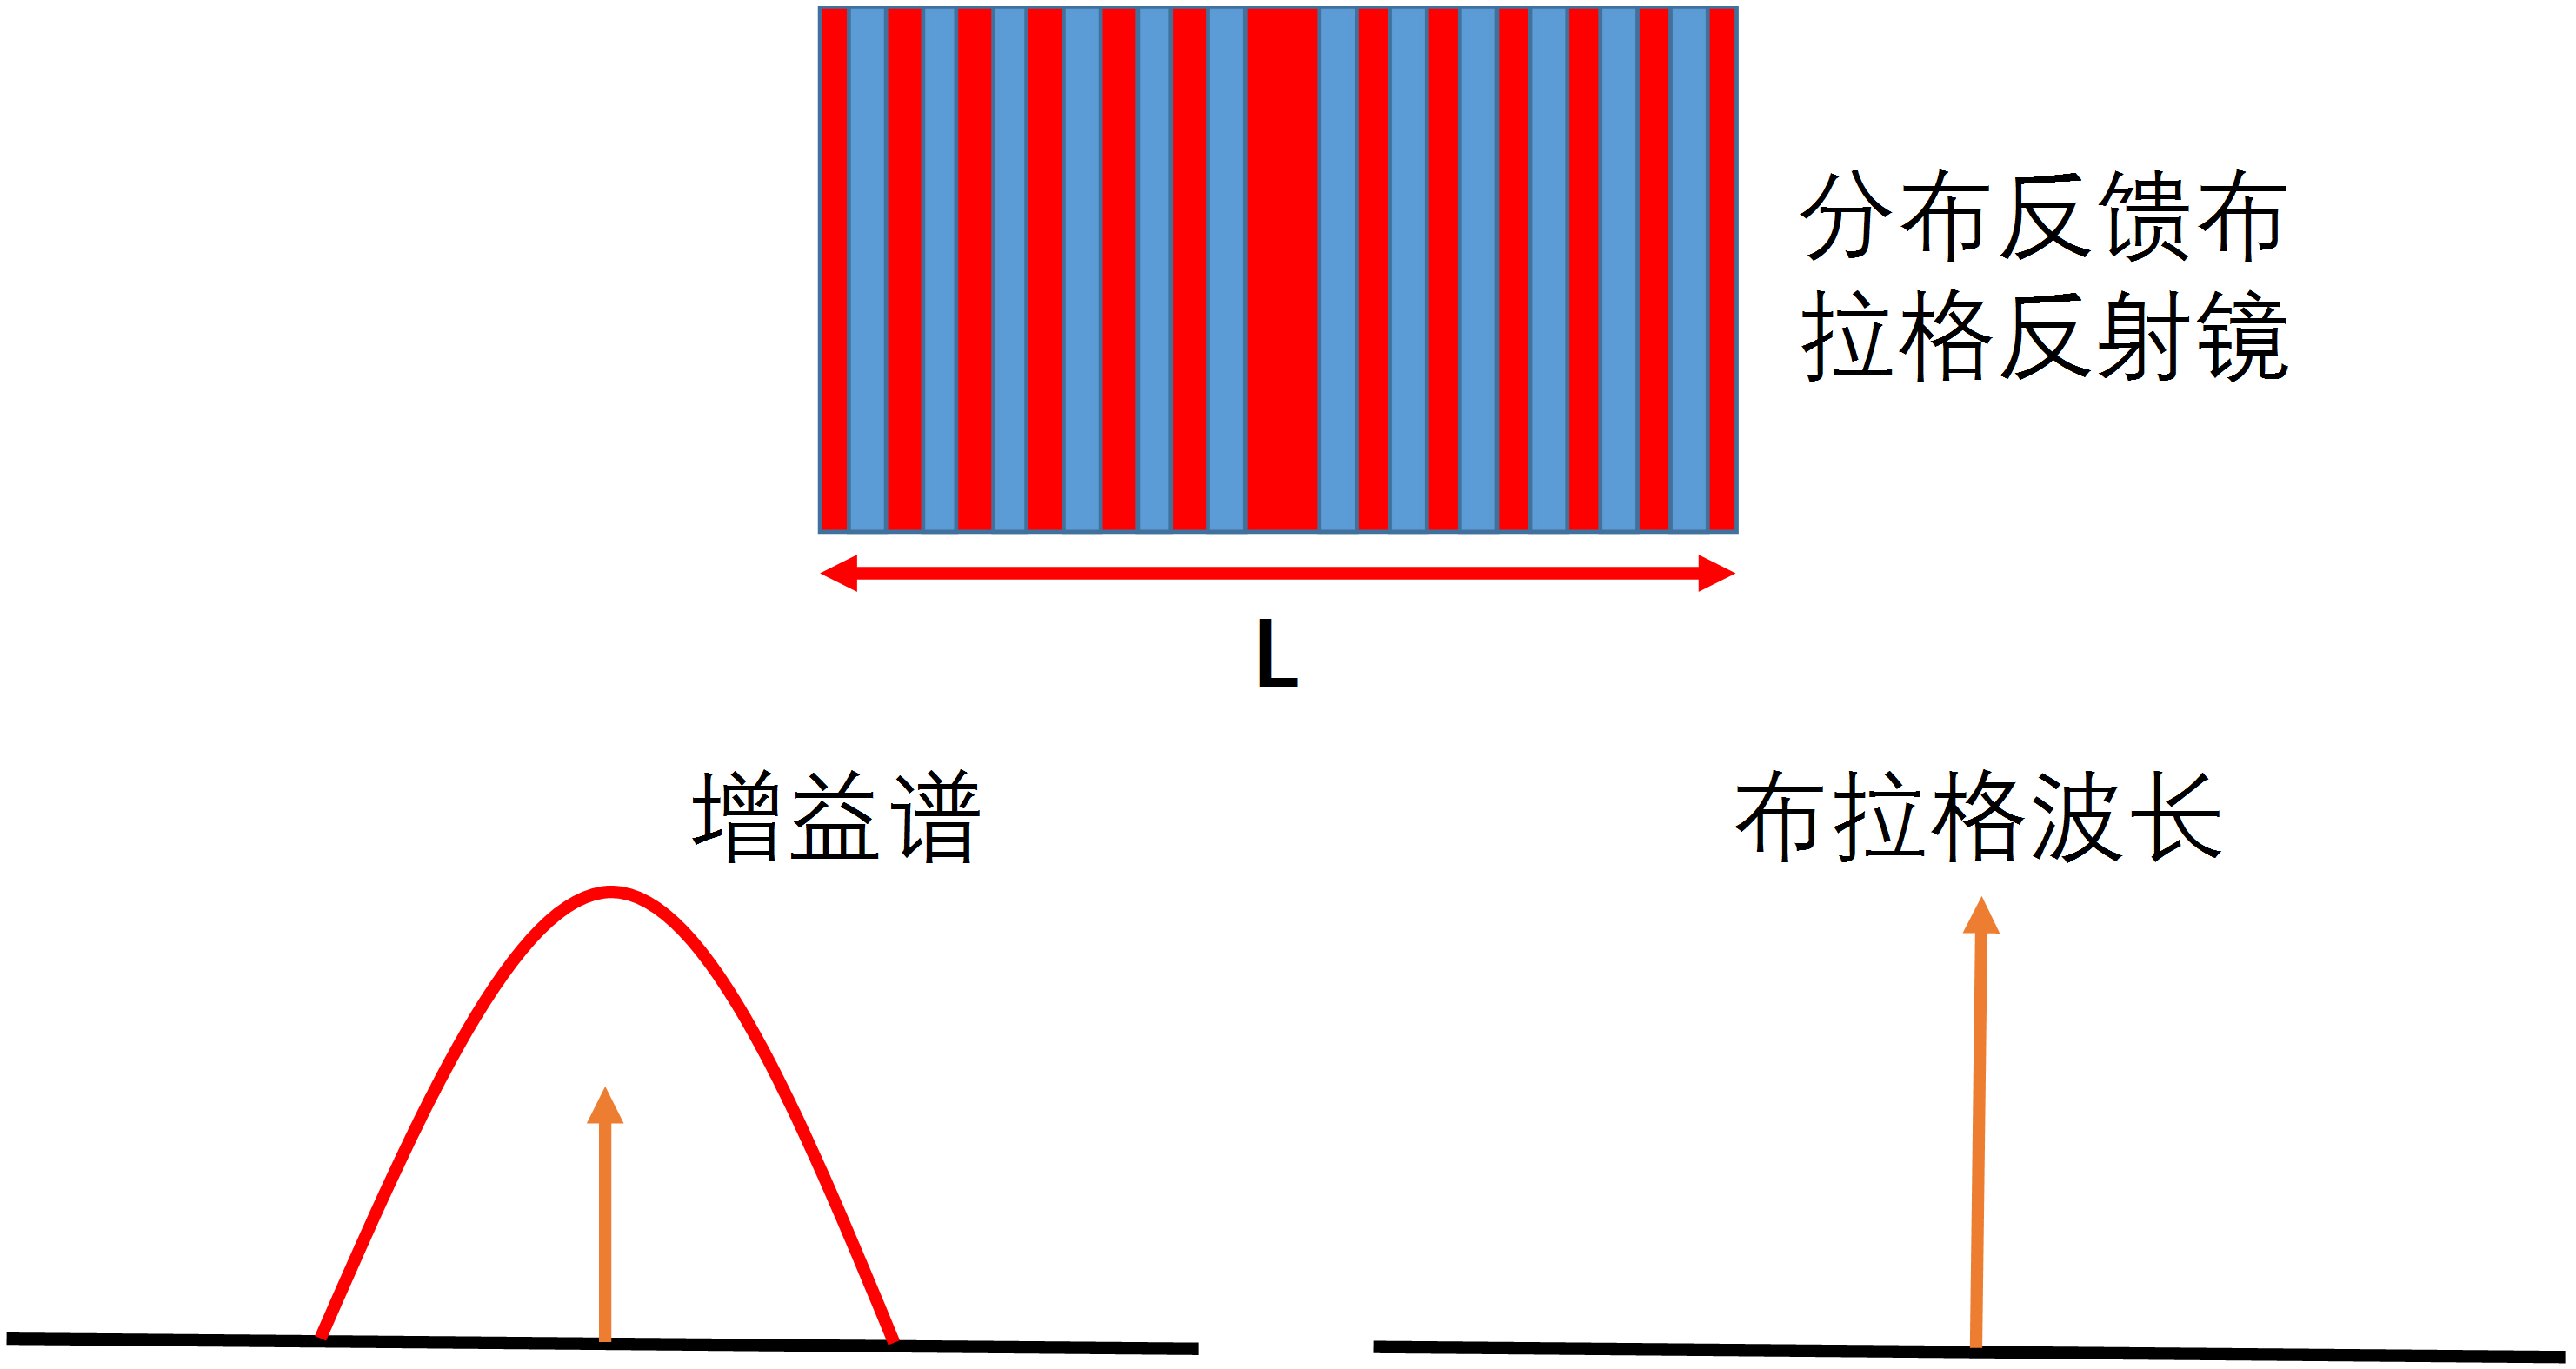
\includegraphics[width=12cm]{./Pictures/fab_dfb_laser.jpg}
	\captionsetup{justification=centering}
	\caption{$\lambda/4$相移DFB激光器激射模式示意图}
	\label{fab_dfb_laser}
\end{figure}

DFB激光器最早由Kogelnik和Shank在上世纪70年代提出\cite{kogelnik1971stimulated,kogelnik1972coupled},然后由Nakamura等人首先在GaAs平台上实现了光泵浦的DFB激光器\cite{nakamura1973optically},之后他们利用双异质结结构在GaAs-GaAlAs平台上实现了电泵浦的DFB激光器\cite{nakamura1974gaas},但这都需要液氮制冷。直到分离限制异质结结构(separate~confinement~heterostructure,~SCH)的提出,Nakamura等人才在GaAs-GaAlAs平台上实现了室温下的连续工作的DFB激光器\cite{nakamura1975cw}。从这以后,DFB激光器吸引了许多研究人员的关注并由于其优异的性能成为了光通信中最主要的光源。为了更深刻理解DFB激光器的工作原理,需要利用速率方程和耦合模理论这两个模型。

\subsection{速率方程}

\subsubsection{载流子密度速率方程}
典型的半导体激光器的截面图如图\ref{laser_activelayer}所示,电流注入端通常采用高掺杂使其与金属形成欧姆接触,有源区不进行掺杂以减小波导的损耗。有源区的载流子密度可以用连续性方程(continuity equations)来描述:
\begin{equation}
\label{continuity_equation}
\left\{
\begin{array}{l}
\dfrac{\partial N(x,y,z,t)}{\partial t} = \dfrac{1}{q}\nabla\cdot J_{n}+G-U\\
\dfrac{\partial P(x,y,z,t)}{\partial t} = -\dfrac{1}{q}\nabla\cdot J_{p}+G-U
\end{array}
\right.
\end{equation}
其中,$J_{n}$和$J_{p}$分别是电子和空穴产生的电流密度,$G$是载流子产生的速度,$U$是载流子复合的速度。对于由折射率差形成有源层波导的激光器来说,我们可以假设电流只在垂直方向传导,在水平方向是均匀的,且由于有源区具有电中性的特点,电子产生的电流应该跟空穴产生的电流相等,故公式\ref{continuity_equation}可以简化为:

\begin{figure}[htb]
	\centering
	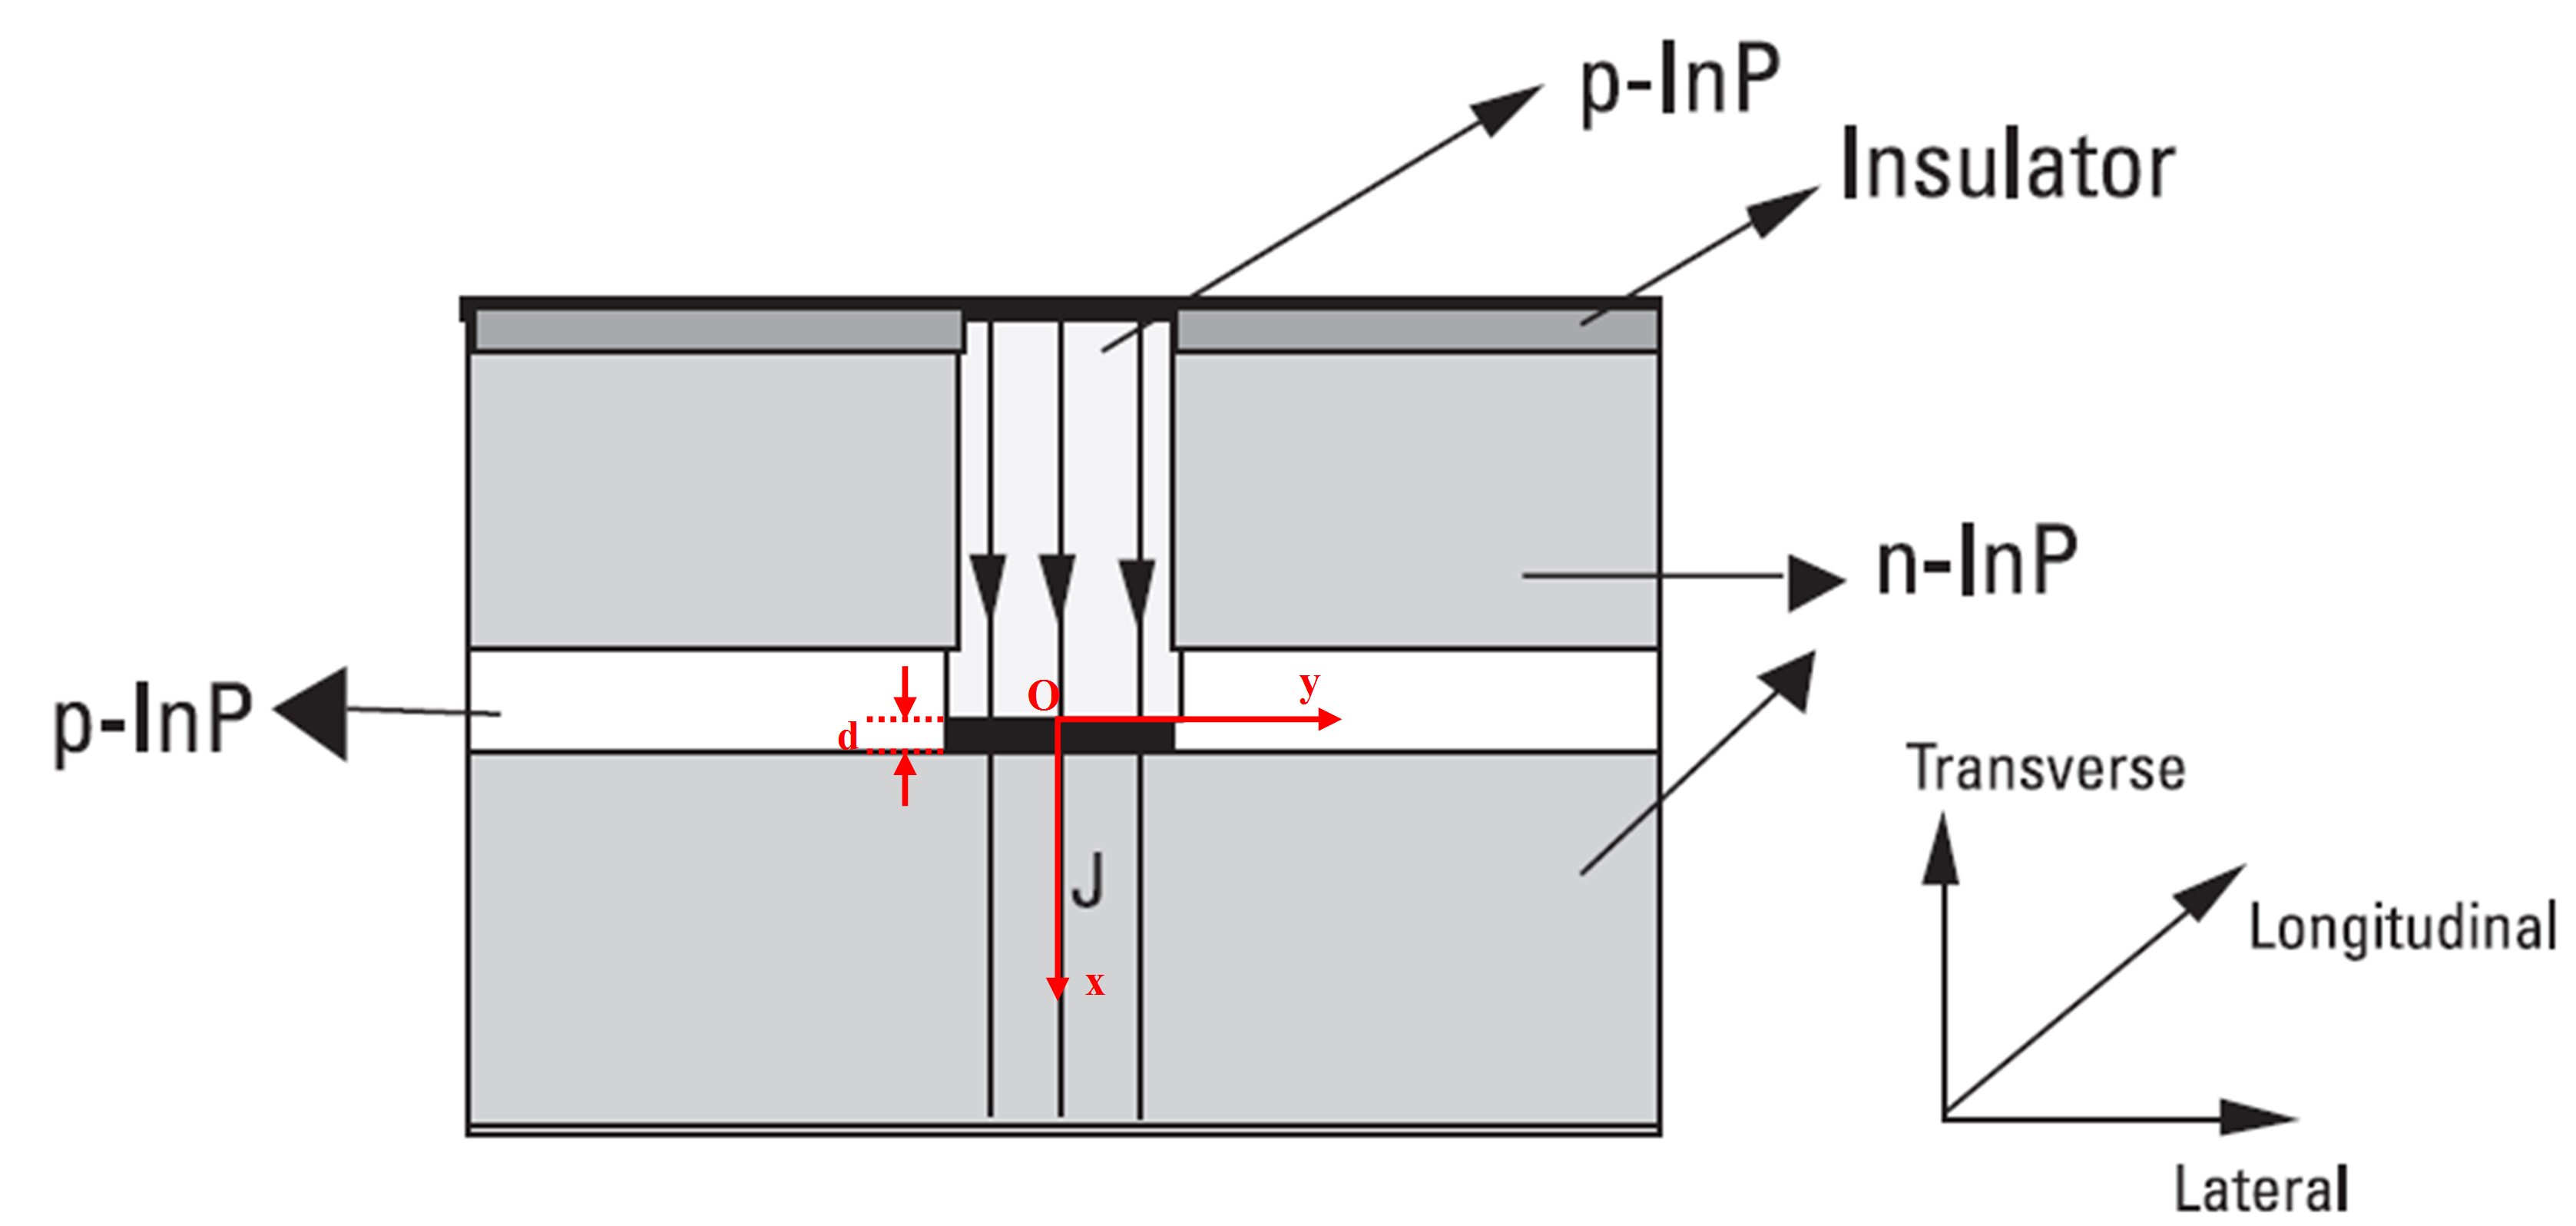
\includegraphics[width=14cm]{./Pictures/laser_activelayer.jpg}
	\captionsetup{justification=centering}
	\caption{典型半导体激光器的截面图\cite{morthier2013handbook}}
	\label{laser_activelayer}
\end{figure}

\begin{equation}
\label{continuity_equation_simplified}
\begin{array}{l}
\dfrac{\partial N(x,y,z,t)}{\partial t} = \dfrac{1}{q}\dfrac{\partial J_{n}}{\partial x}+G-U\\
N = P ~~\text{且}~~ \dfrac{\partial J_{p}}{\partial x} = -\dfrac{\partial J_{n}}{\partial x}~~(0 \le x \le d)
\end{array}
\end{equation}

其中,$x$为垂直的横向方向,原点取有源层波导的上边缘中点,$x$轴的正方向朝下,$d$为有源层的厚度。将公式\ref{continuity_equation_simplified}在有源层进行平均处理,得到平均载流子密度$N$:

\begin{equation}
\label{average_carrier_density}
\dfrac{\partial N}{\partial t} = \dfrac{1}{qd}[J_{n}(d)-J_{n}(0)]+(G-U)_{av}
\end{equation}

其中,$J_{n}(d)$是有源层与n-InP边界处电子产生的电流,$J_{n}(0)$是有源层与p-InP边界处电子产生的电流。由于n-InP有比有源区更大的能带间隔,所以空穴不会从有源区泄漏到n-InP中,同理,电子也不会泄漏到p-InP中,故$J_{n}(d)=J(d)=J$,$J_{n}(0)=0$。如果再将载流子复合,其中包括自发复合和受激辐射复合一起考虑进来,我们最终可以得到载流子的速率方程为:

\begin{equation}
\label{carrier_density_rate_equation}
\dfrac{\partial N}{\partial t} = \dfrac{J}{qd}-AN-BN^{2}-CN^{3}-\sum_{m}G(N,\lambda_{m})S_{m}
\end{equation}

其中,第一项代表有源区载流子的注入并且假设注入效率是100\%;$AN$代表载流子通过表面态或者陷阱产生的自发复合,因为该过程中只有一个载流子参与,故其复合速度与载流子的浓度成正比\cite{shockley1952statistics};$BN^{2}$代表自发辐射复合,因为该过程需要有两个载流子参与,故其复合速度与载流子浓度的平方成正比\cite{olshansky1984measurement};$CN^{3}$代表俄歇复合,电子与空穴复合的能量被另一个电子或者空穴吸收,因此该过程需要有三个载流子参与,故其复合速度与载流子浓度的三次方成正比\cite{agrawal1986long}。俄歇复合的强度与半导体的禁带宽度($E_{g}$)密切相关,$E_{g}$越小,俄歇复合速率就越大,所以俄歇复合对长波长的激光器影响更为严重\cite{dexiu1999};$\sum_{m}$项代表受激辐射复合,求和符号中的$m$代表对所有模式的求和,受激辐射速率与模式的平均光子密度$S_{m}$和增益系数$G(N,\lambda_{m})$成正比。增益系数除了与载流子浓度($N$)和波长($\lambda$)相关外,还与不同模式中的的光子密度($S_{m}$)相关,所以增益系数一般会在光子密度达到一定程度的时候饱和。

\subsubsection{光子密度速率方程}
光子密度速率方程可以根据不同模式中的光子数守恒得到,影响光子密度的过程主要有两个,一是光子的产生,包括受激辐射和自发辐射,二是光子的损耗,包括材料的吸收和反射镜的损耗。其中,受激辐射和损耗与平均光子密度成正比,自发辐射与光子数密度无关,而与载流子密度相关,故光子密度速率方程可以表示为\cite{petermann2012laser}:

\begin{equation}
\label{photon_density_rate_equation}
\dfrac{\partial S_{m}}{\partial t} = [G(N,\lambda_{m})-\gamma_{m}]S_{m}+\dfrac{R_{sp}}{V_{act}}
\end{equation}

其中,$G(N,\lambda_{m})$表示模式增益,对应受激辐射,其与载流子密度和波长相关,$R_{sp}$代表单位时间内耦合进入模式$m$的自发辐射光子数,$S_{m}$代表模式$m$的光子密度,单位为$cm^{-3}$,$\gamma_{m}$代表模式$m$总的损耗,主要包括内部吸收损耗和反射镜损耗:

\begin{equation}
\label{photon_loss}
\gamma_{m} = \gamma_{int}+\gamma_{fac,m} = V_{g,m}(\alpha_{int}+\alpha_{fac,m})
\end{equation}
其中,$\alpha_{int}$是单位长度($cm$)的吸收损耗,$\alpha_{fac,m}$则是模式$m$在两个端面总的损耗,$V_{g,m}$则是对应模式的群速度。

\subsubsection{相位条件}

我们以FP激光器作为例子来简要介绍激光器在谐振时需要满足的相位条件,所得到的结果对DFB激光器也具有参考意义。当光波满足在谐振腔内往返一周所经历的相位变化为2$\pi$的整数倍时,该波长才能满足激射条件。相位条件可以用公式\ref{phase_equation}表达:

\begin{equation}
\label{phase_equation}
2\dfrac{\omega_{m}}{c}n_{eff}(N,\omega_{m})L = 2m\pi
\end{equation}

其中,$m$代表不同的模式,为整数;$L$表示腔长;$\omega_{m}$表示模式的角频率;$n_{eff}$表示模式的等效折射率,其与载流子浓度$N$和角频率$\omega_{m}$相关。将两边同时对$\omega$和$N$微分,公式\ref{phase_equation}可以化为:

\begin{equation}
\label{phase_equation_diff}
\Delta\omega_{m} n_{eff} + \omega_{m} \dfrac{\partial n_{eff}}{\partial \omega} \Delta\omega_{m}+\omega_{m}\dfrac{\partial n_{eff}}{\partial N} \Delta N = 0
\end{equation}

据此,可以得到$\Delta\omega_{m}$与$\Delta N$的关系为:

\begin{equation}
\label{frequency_carrier_relation}
\Delta\omega_{m} = -\dfrac{\omega_{m}}{c}v_{g}\dfrac{\partial n_{eff}}{\partial N} \Delta N = \dfrac{\alpha}{2}\dfrac{\partial G(N,\lambda_{m})}{\partial N} \Delta N 
\end{equation}

公式\ref{frequency_carrier_relation}表示了谐振角频率的偏移量与载流子浓度变化的关系,第二个等式引入的参数$\alpha$,表示线宽增强因子,其与材料和波长相关,通常值为1\~{}5。第二个等式中增益对载流子浓度的微分$\dfrac{\partial G(N,\lambda_{m})}{\partial N}$称为微分增益,通常值为0.5\~{}2 $\times$ 10\SP{18} $cm^{-3}$。

\subsubsection{光学增益}

公式\ref{photon_density_rate_equation}中的模式增益$G(N,\lambda_{m})$与材料增益成正比:
\begin{equation}
\label{modal_gain}
G(N,\lambda_{m}) = \Gamma g(N,\lambda_{m})\nu_g = g_{mod}\nu_g
\end{equation}
其中,$\Gamma$是模式的限制因子,即模式的能量在增益区中所占的比例。$g_{mod}$表示单位距离的增益,乘以群速度$\nu_g$之后就变成了单位时间的增益。

经过前人在理论和实验上的验证,对于体材料来说,其增益与载流子密度成线性关系:
\begin{equation}
\label{bulk_material_gain_equation}
g(N,E) = A(E)N-B(E)
\end{equation}
公式中将$E$取代前面的$\lambda$表示是为了作图的方便,$A(E)$为微分增益,通常值为1\~{}5~$\times$~10\SP{16}~$cm^{2}$,B(E)与透明载流子密度相关,$N_t(E)=B(E)/A(E)$。图\ref{bulk_material_gain}给出了激射波长在1550~$nm$的体材料InGaAsP激光器的增益与载流子密度和光子能量之间的关系。对于应变量子阱材料来说,由于其载流子在某个方向运动受到限制而出现分立的能级,提高了注入有源层内载流子的利用率,可以明显地增加微分增益$A(E)$,从而可以减小激光器的阈值电流,其增益与载流子的关系成亚线性关系:
\begin{equation}
\label{quantum_material_gain}
g = g_0ln\dfrac{N}{N_0}
\end{equation}

\begin{figure}[htb]
	\centering
	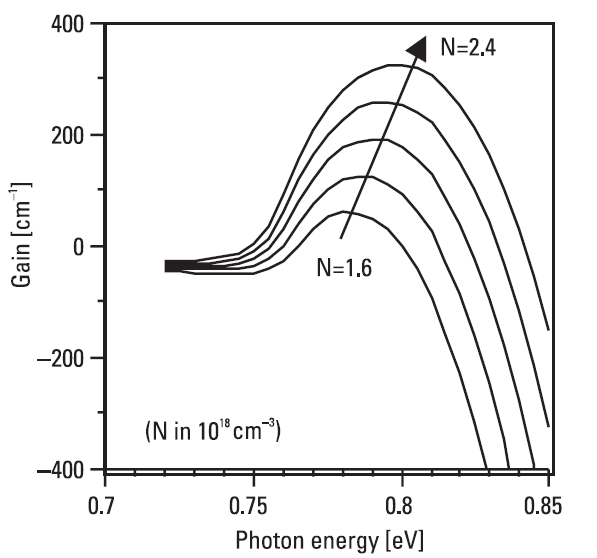
\includegraphics[width=11cm]{./Pictures/fab_bulk_material_gain.png}
	\captionsetup{justification=centering}
	\caption{体材料InGaAsP中增益与载流子密度和光子能量之间的关系\cite{morthier2013handbook}}
	\label{bulk_material_gain}
\end{figure}

\subsection{半导体激光器中的弛豫振荡}
半导体激光器的幅度调制、频率调制可以通过求解载流子密度速率方程和光子密度速率方程得到,在求解过程中,我们假设激光器处于单模工作状态,忽略自发发射,因为与受激辐射的光子数相比,自发辐射的光子数很少。在电流调制的作用下,激光器内的载流子密度$N$、光子密度$S$、电流密度$J$可以表示为:

\begin{equation}
\label{current_modulation}
\begin{array}{l}
N(t) = N_{0}+ Re(N_{1}e^{j\Omega t})\\
N(t) = N_{0}+ Re(N_{1}e^{j\Omega t})\\
N(t) = N_{0}+ Re(N_{1}e^{j\Omega t})
\end{array}
\end{equation}

将其代入载流子密度速率方程\ref{carrier_density_rate_equation}和光子密度速率方程\ref{photon_density_rate_equation},我们只考虑线性项,则可以得到小信号调制下的方程:

\begin{equation}
\label{small_modulation}
\begin{array}{l}
(j\Omega + \dfrac{1}{\tau_{d}} + \dfrac{\partial G}{\partial N}S_{0})N_{1} = \dfrac{J_{1}}{qd} - (G+\dfrac{\partial G}{\partial S}S_{0})S_{1}\\
(j\Omega - \dfrac{\partial G}{\partial S}S_{0})S_{1} = (\dfrac{\partial G}{\partial N}-\dfrac{\partial \gamma}{\partial N})S_{0}N_{1}
\end{array}
\end{equation}

其中,我们忽略了增益的波长相关性,$\tau_{d} = \dfrac{1}{A+2BN_0 +3CN_0^2}$表示微分载流子寿命。通过公式\ref{small_modulation}容易解得$S_{1}$与$N_{1}$,其中$S_{1}$就对应强度调制的响应,$N_{1}$通过与公式\ref{frequency_carrier_relation}就可以得到频率调制的响应:

\begin{equation}
\label{am_fm}
\begin{array}{l}
S_{1} = \dfrac{(\dfrac{\partial G}{\partial N}-\dfrac{\partial\gamma}{\partial N})S_{0}\dfrac{J_{1}}{qd}}{(j\Omega-\dfrac{\partial G}{\partial S}S_{0})(j\Omega+\dfrac{1}{\tau_{d}}+\dfrac{\partial G}{\partial N}S_{0})+G(\dfrac{\partial G}{\partial N}-\dfrac{\partial\gamma}{\partial N})S_{0}}\\
\Delta\omega = \dfrac{\alpha}{2}\dfrac{\partial G}{\partial N}\dfrac{(j\Omega+\dfrac{\partial G}{\partial S}S_{0})\dfrac{J_{1}}{qd}}{(j\Omega-\dfrac{\partial G}{\partial S}S_{0})(j\Omega+\dfrac{1}{\tau_{d}}+\dfrac{\partial G}{\partial N}S_{0})+G(\dfrac{\partial G}{\partial N}-\dfrac{\partial\gamma}{\partial N})S_{0}}
\end{array}
\end{equation}

从中,我们可以看到强度调制与频率调制的响应与调制的频率相关,且其相互之间通过载流子的动态过程相互耦合,故对激光器进行强度调制时,往往也伴随着频率调制(啁啾现象),这也是限制直调激光器在光通信系统中使用的因素之一。为了减小啁啾现象,可以通过减小线宽增强因子$\alpha$来实现。多量子阱激光器相比于体材料有更小的线宽增强因子,故其更适用于制作直调激光器。图\ref{laser_amfm_response}展示了典型的强度调制和频率调制的频率响应图。

\begin{figure}[htb]
	\centering
	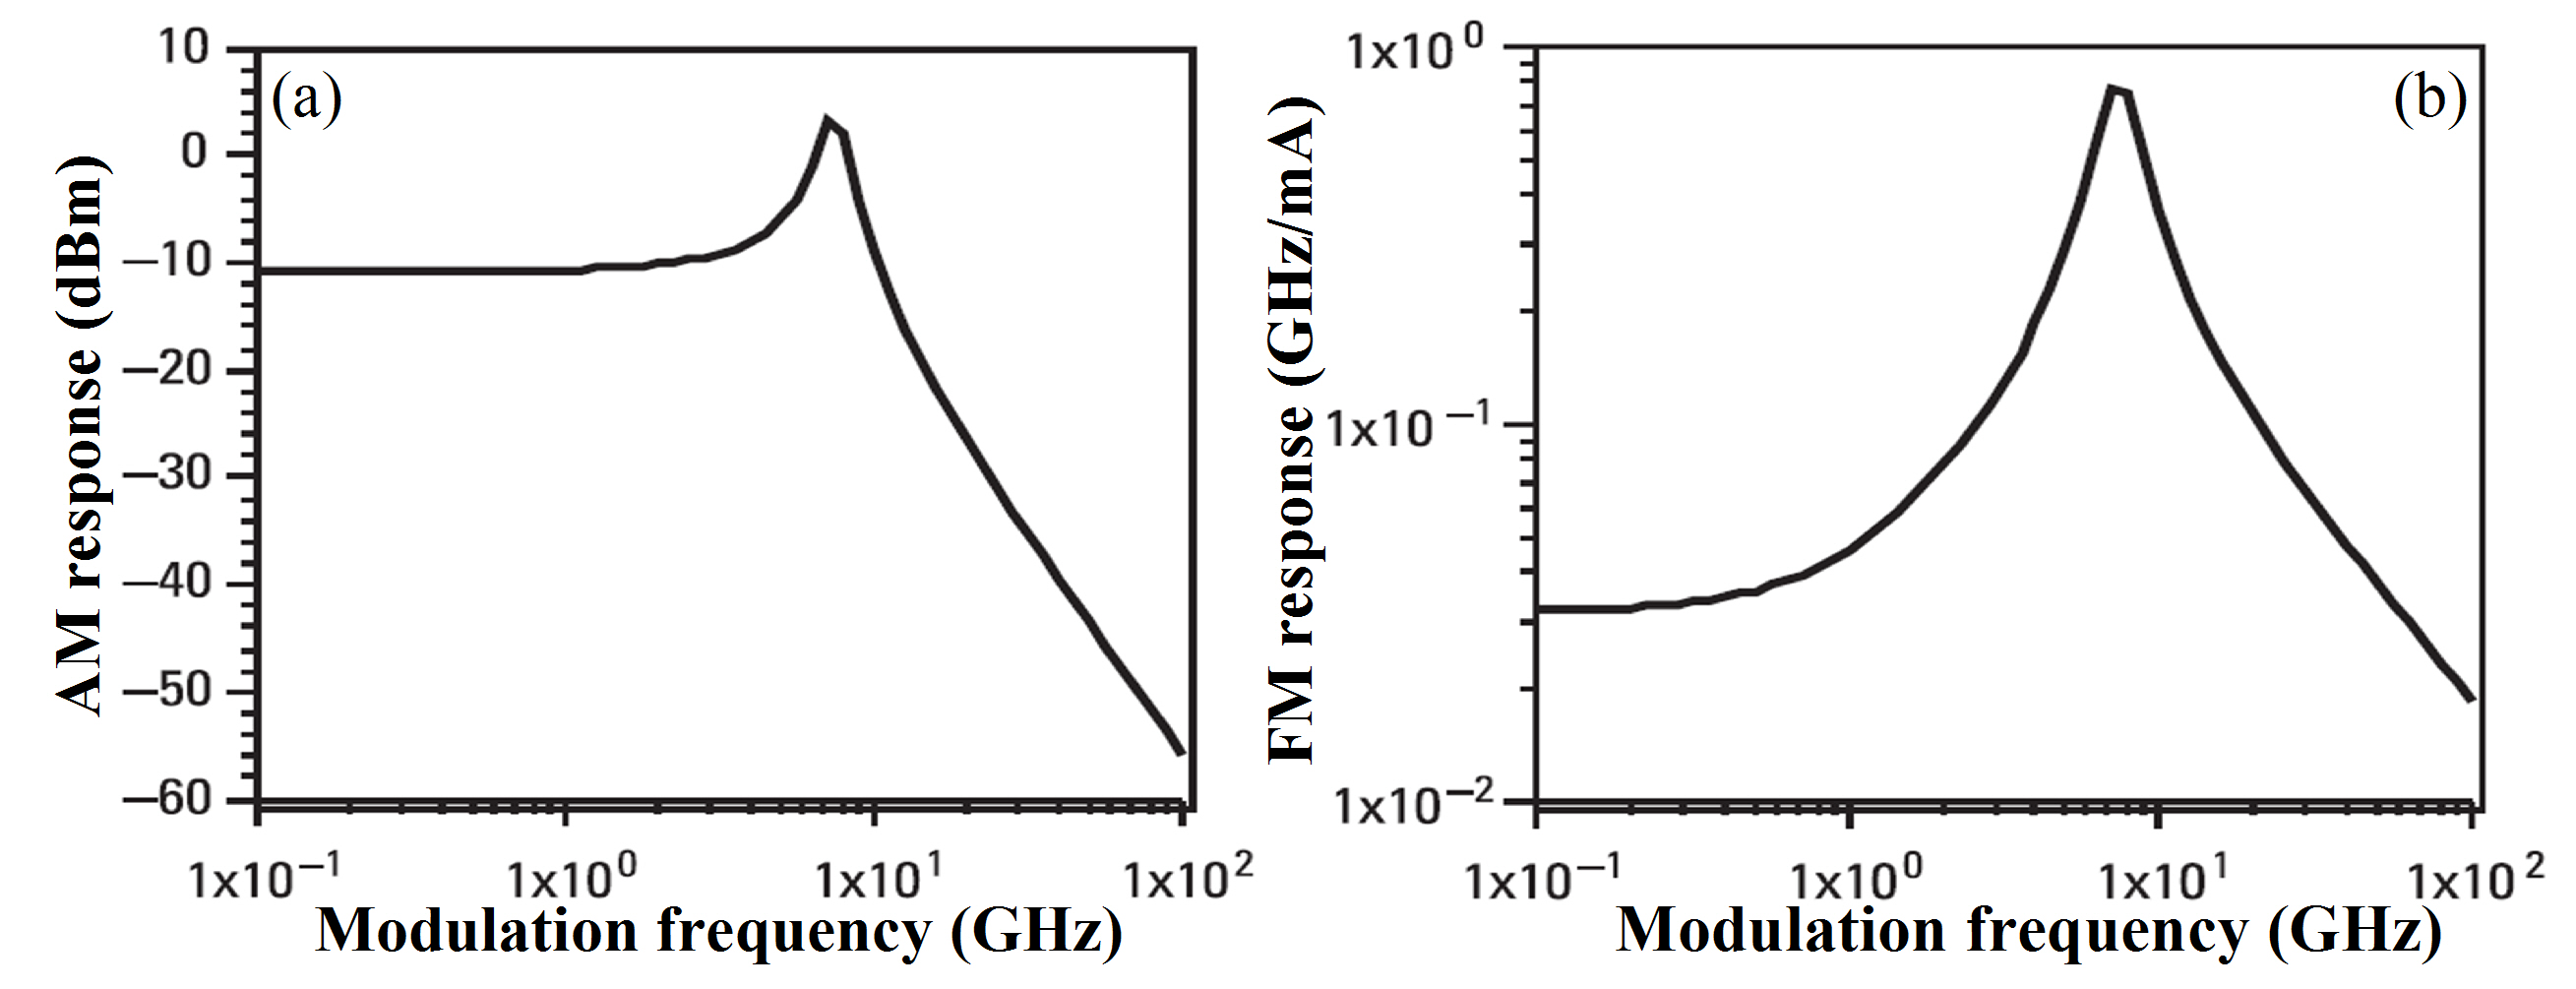
\includegraphics[width=16cm]{./Pictures/laser_amfm_response.jpg}
	\captionsetup{justification=centering}
	\caption{典型的强度调制和频率调制的频率响应;(a)幅度调制响应;(b)频率调制响应\cite{morthier2013handbook}}
	\label{laser_amfm_response}
\end{figure}

从中我们可以看到明显的谐振现象,一般把这种在半导体激光器中,由于驱动电流调制所产生的谐振现象称为激光器的驰豫振荡,其谐振频率$f_{r}$与阻尼系数$\theta$可由公式\ref{relaxation_oscillation}得到,其所对应的物理过程为载流子与光子之间通过受激辐射和受激吸收这两个过程进行能量交换。在稳态条件下,调制电流注入一部分载流子,使得此时激光器的增益会大于损耗,受激辐射就会产生更多的光子。但是随着光子数的增多消耗了激光器内的载流子,使其浓度下降,导致激光器的增益小于损耗,然后光子数又会减少,受激辐射就会减弱,使得载流子浓度又得以升高,如此往复。由于弛豫振荡现象的存在,导致激光器在调制的过程中当调制频率大于弛豫振荡的频率时,信号会出现畸变,这就限制了激光器调制速率的上限。

\begin{equation}
\label{relaxation_oscillation}
\begin{array}{l}
(2\pi f_{r})^{2} = G_{th}(\dfrac{\partial G}{\partial N}-\dfrac{\partial\gamma}{\partial N})S_{0} \approx \dfrac{\partial G}{\partial N}\dfrac{I-I_{th}}{qV_{act}}\\
\theta = \dfrac{1}{\tau_{d}} + \dfrac{\partial G}{\partial N}S_{0}+\dfrac{\partial G}{\partial S}S_{0}
\end{array}
\end{equation}

从公式\ref{relaxation_oscillation}中我们可以看到,弛豫振荡频率与阻尼系数都随着稳态时的光子密度和微分增益的增加而增加,因为其可以加快光子与电子之间能量交换的速率。而且,通过增加模式限制因子,缩小有源区的体积也可以增加驰豫振荡的频率,通常谐振频率处于几个GHz到10几个GHz之间。

\subsection{耦合模理论}

DFB激光器是一个非常复杂的系统,其包括电、光、热之间的非线性耦合过程。想要将所有过程都详细地讨论是不现实的,但是过于简化的模型也不适用于解释DFB激光器的各种物理现象,耦合模理论提供了这样一种平衡,其可以用来分析DFB激光器中载流子密度与光子密度的分布问题。

DFB激光器中的光场可以表示成正向传输的光场$F(z)$和反向传输的光场$B(z)$之和:
\begin{equation}
\label{field_sum}
E(z) = F(z)exp(i\beta z) + B(z)exp(-i\beta z)
\end{equation}
其中,$\beta$为模式的传播常数。正向传输的光场$F(z)$和反向传输的光场$B(z)$通过DFB光栅会互相耦合,耦合系数$\kappa$与光栅的折射率的变化量$\Delta n$成正比,耦合方程可以写为:
\begin{equation}
\label{coupling_dfb1}
\dfrac{dF(z)}{dz} = (\gamma-j\Delta \beta)F(z)-j\kappa B(z)
\end{equation}
\begin{equation}
\label{coupling_dfb2}
\dfrac{dB(z)}{dz} = -(\gamma-j\Delta \beta)B(z)-j\kappa F(z)
\end{equation}
其中,$\gamma$表示模式的增益,$\Delta\beta$表示传播常数与布拉格波矢之间的失谐因子:
\begin{equation}
\label{delta_beta}
\Delta\beta = \dfrac{2\pi n_{eff}}{\lambda} - \dfrac{\pi}{\Lambda}
\end{equation}
其中,$\Lambda$为布拉格光栅的周期。

有了$F(z)$和$B(z)$的耦合方程之后,结合$z=z_0$处给定的初始条件,可以求得任意坐标处的值,其结果可以表示为:
\begin{equation}
\label{coupling_result}
\left[\begin{matrix}
F(z) \\
B(z)
\end{matrix}\right] = \left[\begin{matrix}
cosh(Sz)+\dfrac{\gamma-j\Delta\beta}{S}sinh(Sz) & -\dfrac{j\kappa}{S}sinh(Sz) \\ 
-\dfrac{j\kappa}{S}sinh(Sz) & cosh(Sz)-\dfrac{\gamma-j\Delta\beta}{S}sinh(Sz)
\end{matrix}\right]\left[\begin{matrix}
F(z_0)\\
B(z_0)
\end{matrix}\right]
\end{equation}
其中,$S^2 = \kappa^2+(\gamma-j\Delta\beta)^2$。该矩阵也叫做$z$与$z_0$之间的传输矩阵$T$,如果我们考虑DFB激光器两边都镀上减反膜,即两边的反射率为零。并且让$z=L$,$z_0=0$,利用边界条件可以求得$T_{22}=0$,即:
\begin{equation}
\label{boudary_condition_result}
SLcoth(SL) - \gamma L + j\Delta\beta L = 0
\end{equation}

通过数值方法求解公式\ref{boudary_condition_result}可以得到不同耦合系数下模式增益$\gamma L$与$\Delta\beta L$之间的关系如图\ref{fab_stopband}(a)所示,从中可以看出,对于中心无$\lambda/4$相移的DFB激光器来说,其在失谐因子$\Delta\beta L=0$处即布拉格波长处没有模式,其两个一阶模式对称分布在布拉格波长两边,它们之间的距离称之为DFB激光器的阻带宽度,可以反映激光器的耦合强度,耦合强度越强,阻带宽度也就越大,对于没有增益与损耗的布拉格光栅来说,其关系如公式\ref{stopband_coupling_coefficient}所示:
\begin{equation}
\label{stopband_coupling_coefficient}
\Delta\lambda = \dfrac{\lambda_\beta^2}{\pi n_{eff}L}\sqrt{(\kappa L)^2+\pi^2}
\end{equation}

由于这两个一阶模式拥有相同的阈值增益,故该类DFB激光器往往具有多模特性。这两个一阶模式的简并可以通过图\ref{fab_lambda_4_explanation}进行解释,观察$z_1$与$z_2$处反射波的相位叠加,由于光场经过$\Lambda/2$距离的传输,相位变化为$\pi/2$,所以每个光栅界面反射的光波相位差在$0$和$\pi$之间变化,$z_1$与$z_2$处的光场叠加将处于干涉相长状态。如果DFB光栅中心无$\lambda/4$的相移,则经过$\Lambda/2$距离的传输,相位差将变为$(2p+1)\pi$,其中$p$为整数,故在布拉格波长处无模式存在。

\begin{figure}[htb]
	\centering
	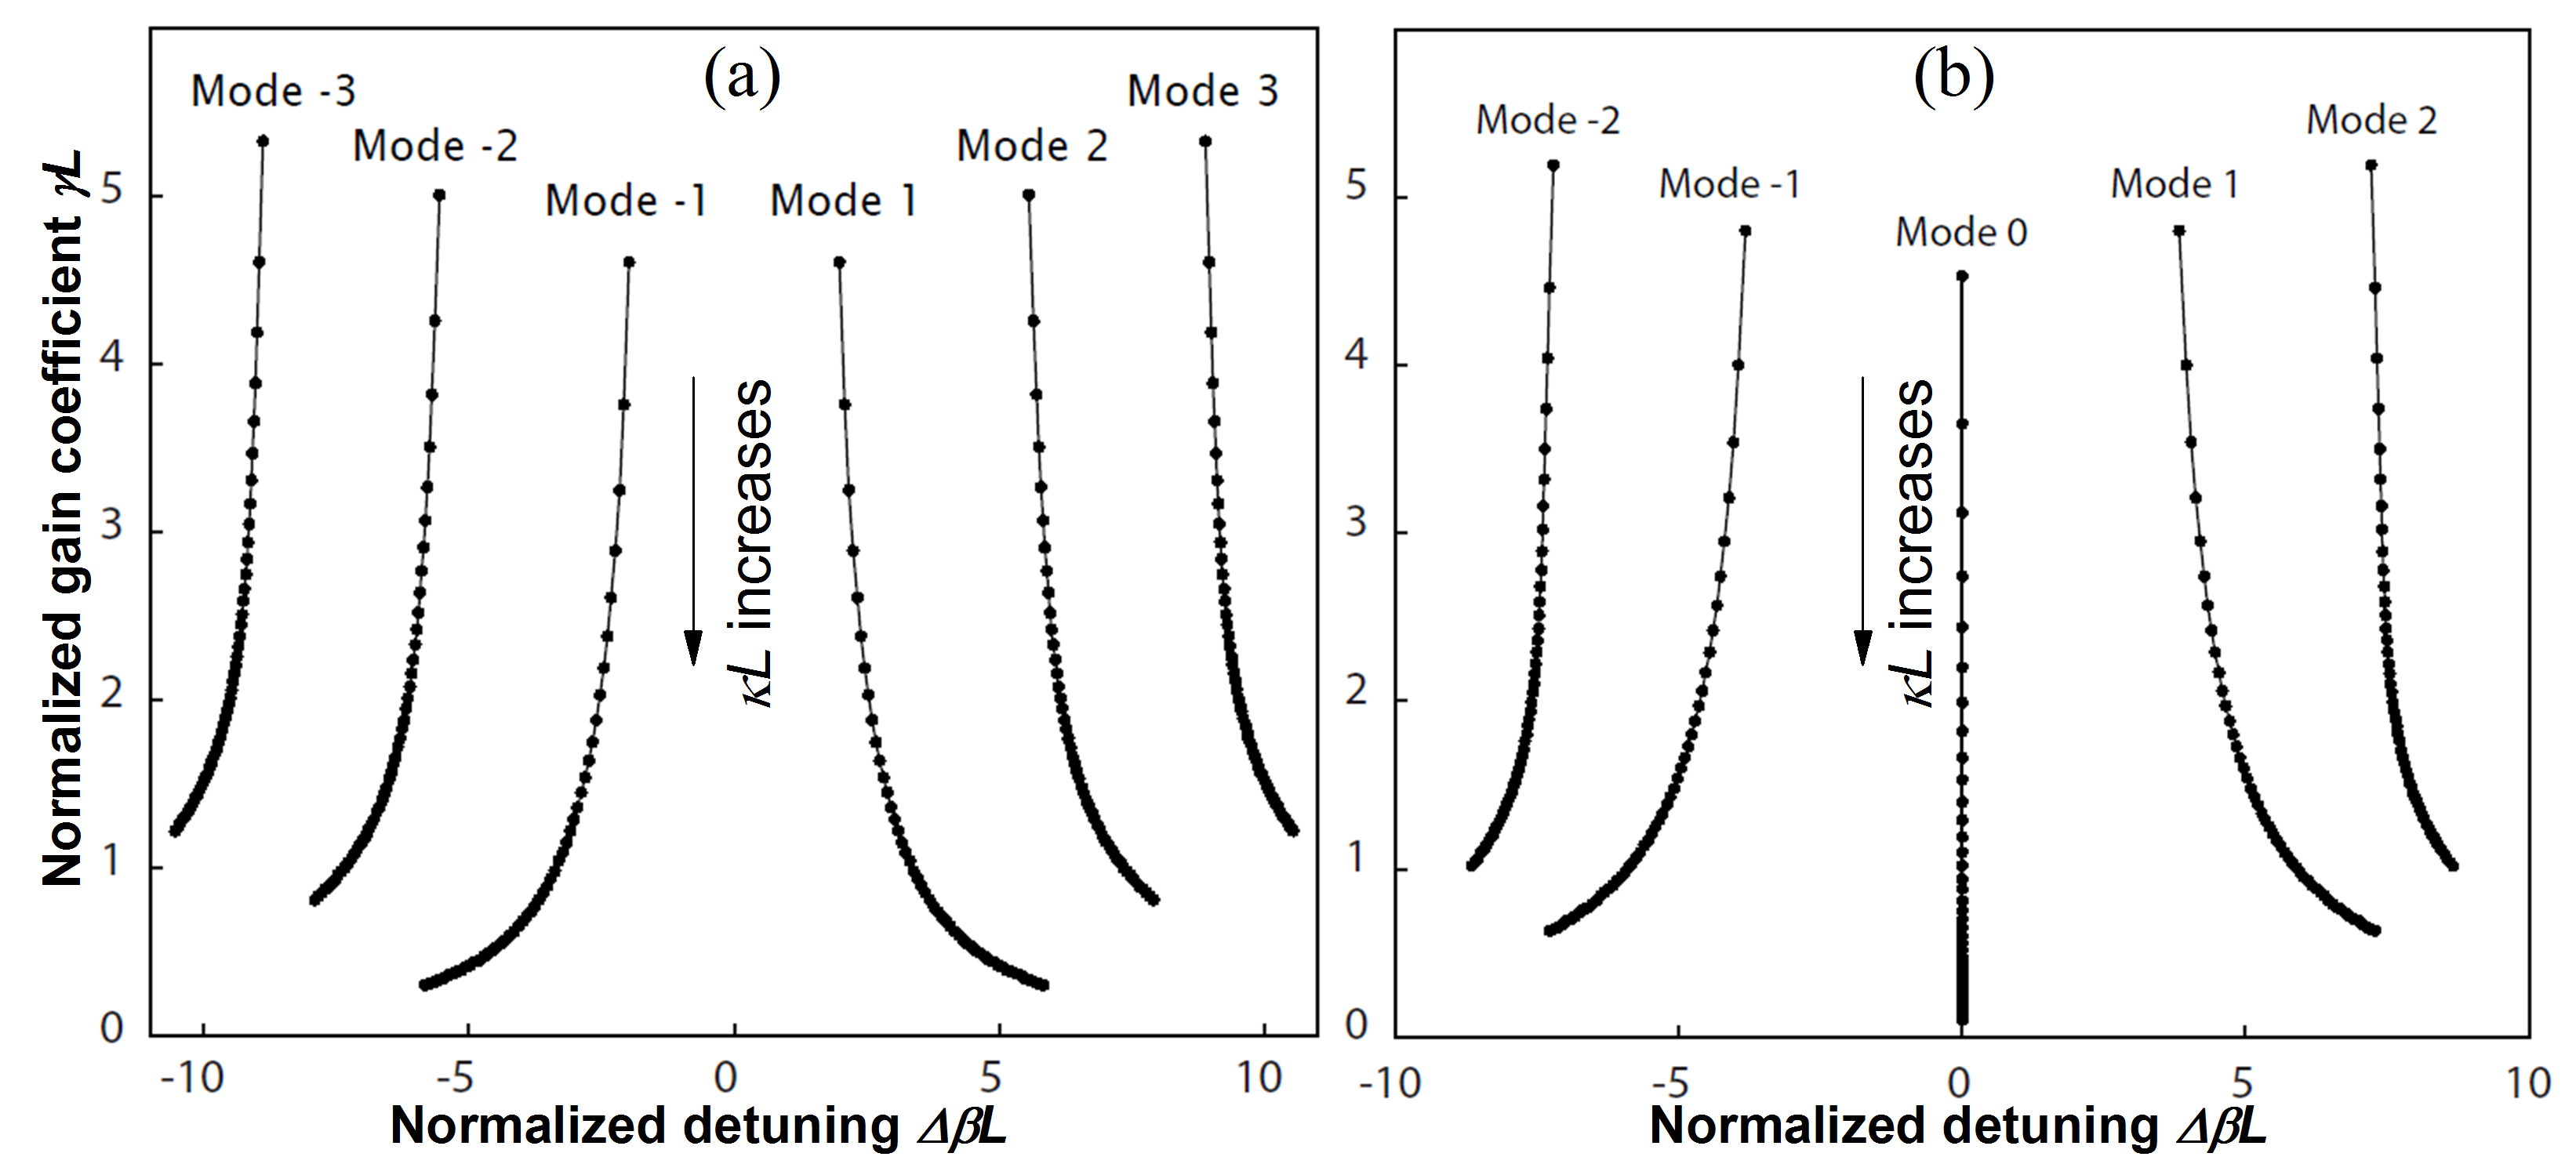
\includegraphics[width=16cm]{./Pictures/fab_stopband.jpg}
	\captionsetup{justification=centering}
	\caption{不同归一化耦合强度$\kappa L$下,归一化阈值增益与归一化失谐因子之间的关系,(a)中心无$\lambda/4$相移的DFB激光器;(b)中心有$\lambda/4$相移的DFB激光器\cite{huybrechts2010digital}}
	\label{fab_stopband}
\end{figure}

\begin{figure}[htb]
	\centering
	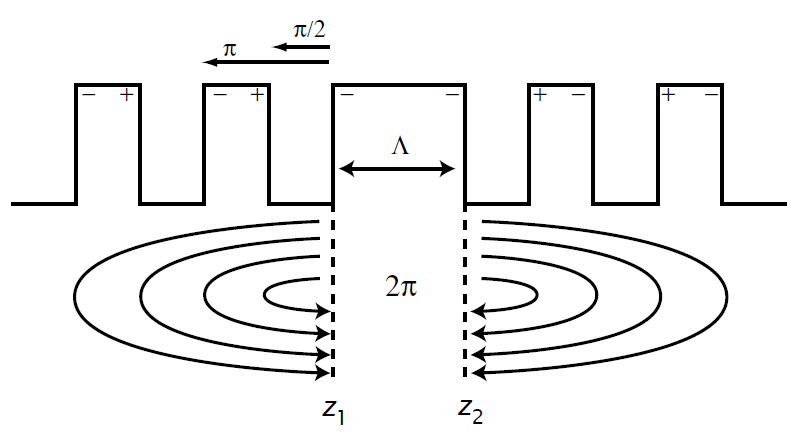
\includegraphics[width=12cm]{./Pictures/fab_multimode_explanation.png}
	\captionsetup{justification=centering}
	\caption{DFB光栅中央处$\lambda/4$相移作用的物理解释\cite{morthier2013handbook}}
	\label{fab_lambda_4_explanation}
\end{figure}

要解决这个问题,可以在DFB光栅中心加入$\lambda/4$的相移,此时就可以将$z_1$与$z_2$处的光场增加额外的$\pi$相位,从而消除模式简并。添加$\lambda/4$的相移之后,DFB激光器的传输矩阵可以变为$T(L/2)T(\Lambda/2)T(L/2)$,公式\ref{boudary_condition_result}变为:
\begin{equation}
\label{boudary_condition_result2}
SLcoth(SL/2) - (\gamma L - j\Delta\beta L \pm \kappa L) = 0
\end{equation}
利用数值方法求解公式\ref{boudary_condition_result2}得到不同耦合系数下模式增益$\gamma L$与$\Delta\beta L$之间的关系如图\ref{fab_stopband}(b)所示,此时在布拉格波长处的模式的阈值增益最小,故我们可以知道,两边镀减反膜且中心加入$\lambda/4$相移的DFB激光器可以实现单模激射。



\section{光子器件基本制作工艺}
得益于SOI平台的高折射率差,硅基光电子器件的特征尺寸在亚微米量级,最常见的单模波导,其宽度为500~$nm$,如果采用狭缝结构的波导,其狭缝的宽度则只有100~$nm$左右。对于片上的一阶布拉格反射镜,其周期在400~$nm$左右,所以其单个光栅的尺寸也在200~$nm$左右,对于一维光子晶体纳米梁腔,其特征尺寸更小。普通的接触式光刻已经无法满足如此高的加工精度要求,所以制作这类器件常常需要使用电子束曝光(electro-beam lithography, EBL)来完成器件的制作。基于电子束曝光的硅基光子器件制作过程通常包括SOI芯片的清洗与匀胶、电子束曝光与显影、刻蚀等工艺流程,下面主要介绍以上主要工艺流程。

\subsection{SOI芯片的清洗与匀胶}
我们以220~$nm$~SOI(SOITEC Inc.)芯片为例,来介绍硅光子学器件的基本工艺流程。解理完合适大小的SOI芯片后,一般为1.5~$cm$~$\times$~1.5~$cm$,方便工艺过程中用镊子进行操作。解理完之后芯片表面一般如图\ref{fab_surface}所示,可以看到SOI芯片表面会吸附很多有机物等杂质,所以需要对其进行清洗。
\begin{figure}[htb]
	\centering
	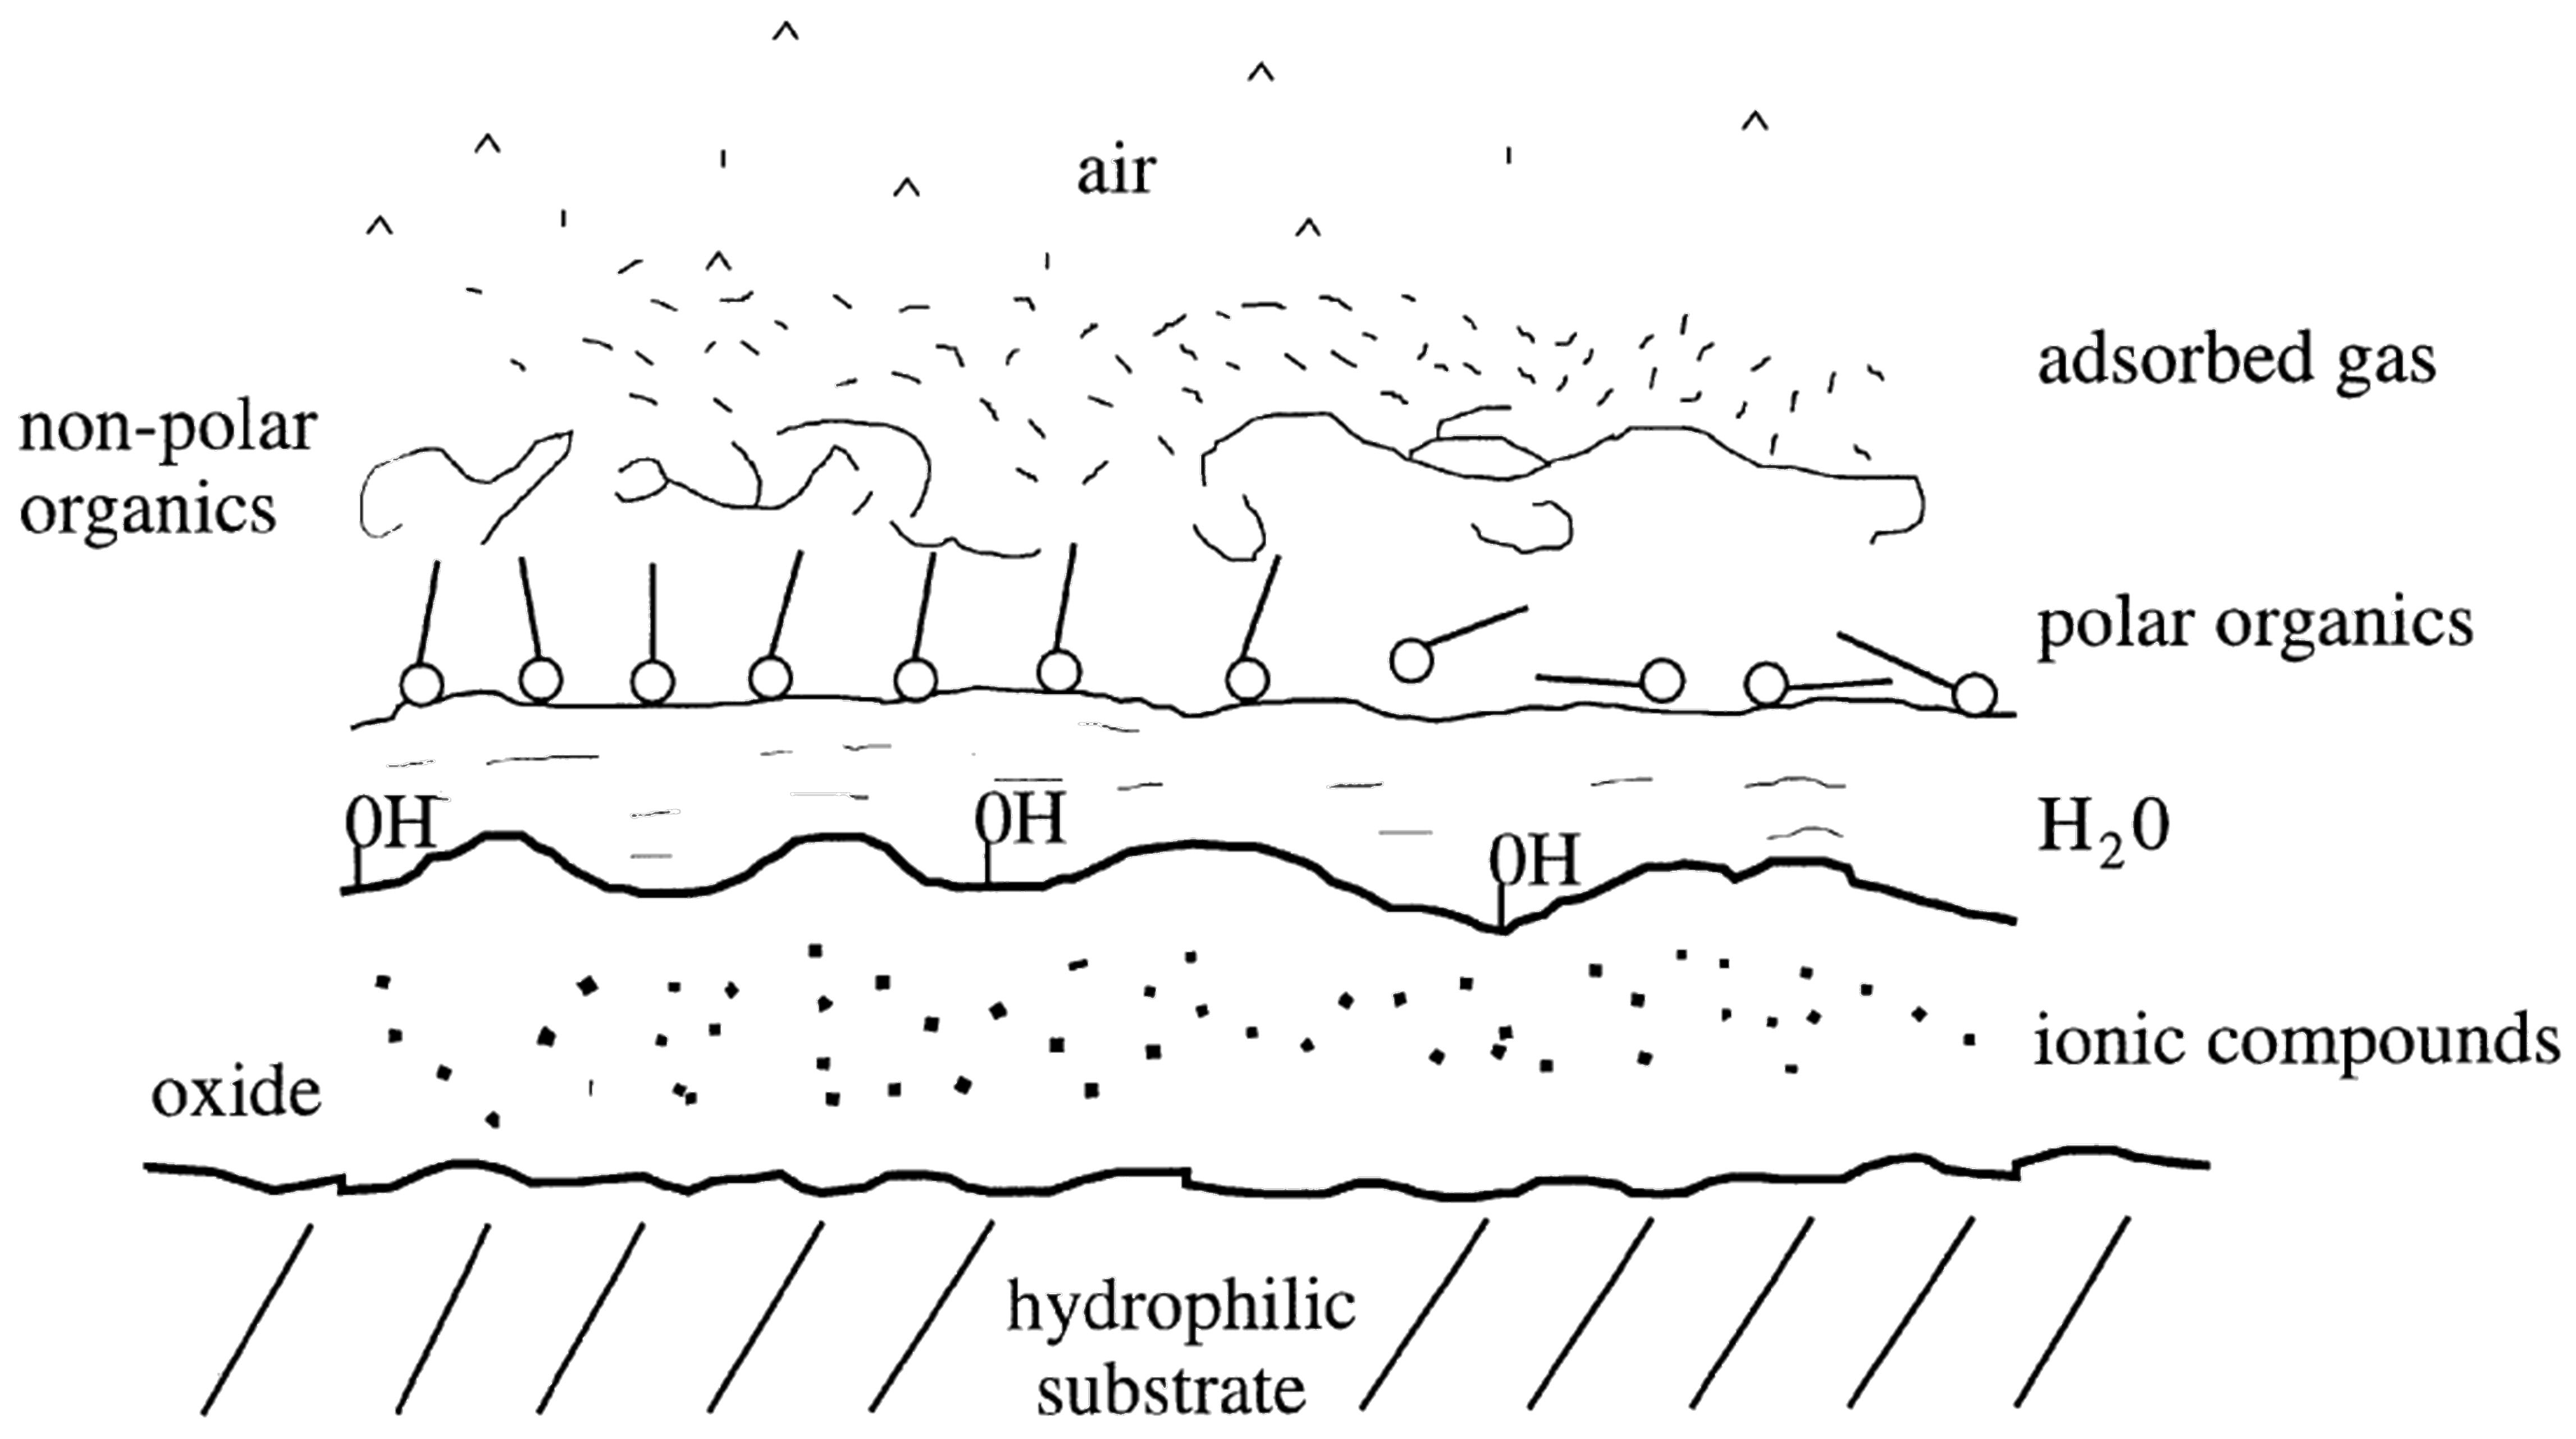
\includegraphics[width=14cm]{./Pictures/fab_surface.jpg}
	\captionsetup{justification=centering}
	\caption{亲水表面通常会吸附的物质\cite{plossl1999wafer}}
	\label{fab_surface}
\end{figure}

主要的清洗步骤为:
\begin{enumerate}[(1)]
	\item 
	用氮气枪吹扫SOI芯片表面,去除可能因解理时落在上面的硅小颗粒,不宜用较强的气流,否则硅小颗粒有可能划伤SOI芯片的表面。
	\item 
	由于SOI芯片表面往往会吸附有机物杂质,故需要用丙酮、甲醇、异丙醇分别超声清洗5~$min$,去除有机物杂质。
	\item 
	将SOI芯片用浓H\SB{2}SO\SB{4}:H\SB{2}O\SB{2}=1:1(体积比)的食人鱼溶液浸泡2~\~{}3小时,该步骤是为了去除表面的残留有机物。用其他比例也是可以的,它们还是可以被叫做食人鱼溶液。浸泡食人鱼溶液之前一定要将前一步有机物去除干净,只允许有非常少的残留,否则有可能会引起爆炸。
	\item 
	经过食人鱼溶液处理过后的SOI表面会被羟基(-OH)化,芯片表面会变成亲水性。由于我们使用的电子束光刻胶一般都属于有机试剂,故经过食人鱼溶液处理的SOI芯片直接进行匀胶的话,胶与芯片表面的粘附性往往不够好,故需要将SOI芯片在氢氟酸缓冲液(buffered oxide etch, BOE)中浸泡10~$s$左右,以去除表面的羟基(-OH),其组成为NH\SB{4}F:HF~=~6:1。随后用去离子水清洗干净之后,置于热板上烘干。
\end{enumerate}

完成以上清洗步骤之后,就可以准备将电子束光刻胶(又可以称为电子束抗蚀剂)旋涂到SOI芯片表面。对于电子束光刻胶,可以分为正胶和负胶,对于正胶来说,经过电子束曝光使得光刻胶中原本存在的交联断裂,在之后的显影过程中容易被溶解掉;对于负胶来说,电子束曝光使得光刻胶中的小分子发生交联,在之后的显影过程中不容易被溶解。实验室常用的正胶有聚异丁烯酸甲酯(Polymethylmethacrylate, PMMA),ZEP 520A(主要由$\alpha$-氯代甲基丙烯酸酯和$\alpha$-甲基苯乙烯的共聚物组成),负胶有ma-N2400系列等。几种常用的电子束光刻胶使用参数如表\ref{ebeamresist}所示:

\begin{table}[htb]
	\zihao{5}
	\captionsetup{justification=centering}
	\caption{实验室常用的三种电子束光刻胶及其各项参数}
	\label{ebeamresist}
	\centering
	\begin{tabular}[t]{cccccccc}
		\hline
		\textbf{光刻胶} & \textbf{转速(r/min)}  & \textbf{前烘} & \textbf{显影(s)} & \textbf{定影(s)} & \textbf{坚膜} & \textbf{剂量(30kV)} \\
		\hline
		PMMA & 4000 &  180$^{\circ}$C~10~$min$ & 35 & 35 & 90$^{\circ}$C~10~$min$ & 300 \\
		\hline
		ZEP 520A & 6000 &  180$^{\circ}$C~10~$min$ & 40 & 60 & 120$^{\circ}$C~10~$min$ & 95 \\
		\hline
		ma-N 2403 & 4000 &  90$^{\circ}$C~90~$s$ & 150 & null & 110$^{\circ}$C~40~$min$ & 130 \\
		\hline
	\end{tabular}
\end{table}

匀胶是将液态粘稠的光刻胶通过快速旋转,借助离心力均匀地涂覆到SOI芯片上的过程,光刻胶的厚度可以根据光刻胶浓度与转速控制,达到想要的厚度。决定匀胶厚度时,常常需要考虑到光刻胶与硅的刻蚀比,对于PMMA来说,其与硅的刻蚀比在1:1\~{}2左右,即刻蚀1~$nm$~PMMA,可以刻蚀1\~{}2~$nm$的硅。对于ZEP 520A,刻蚀比可以达到1:4,故其可以用来制作刻蚀深度更大的器件。图\ref{fab_spinner}为实验室所使用的匀胶机。

\begin{figure}[htb]
	\centering
	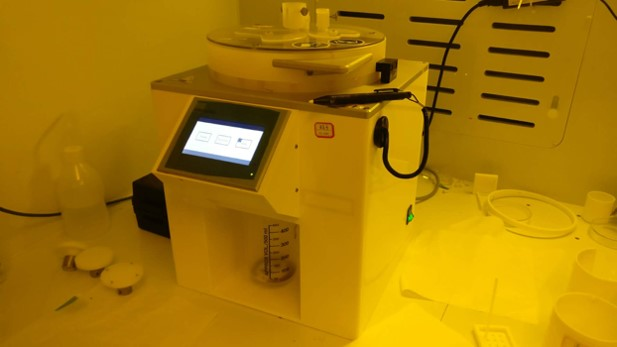
\includegraphics[width=12cm]{./Pictures/fab_spinner.jpg}
	\captionsetup{justification=centering}
	\caption{SUSS Micro Tec 公司的Labspin6匀胶机}
	\label{fab_spinner}
\end{figure}
匀胶的具体过程如下:
\begin{enumerate}
	\item 
	将SOI芯片置于匀胶机吸盘中央并使吸盘处于抽真空状态,使得芯片被固定住以防在高速旋转式被甩出去,污染芯片。此步往往需要借助蓝膜增加气密性。
	\item 
	设置好匀胶机的参数,一般包括前转和后转,其中前转主要是为了控制开始旋转的加速过程,以便光刻胶能够能够较为快速地分布到整块SOI芯片上,但如果前转速度太快,会导致光刻胶直接被甩飞出去,无法形成均匀的覆盖。后转是为了让SOI芯片上的各处光刻胶厚度尽量均匀一致。以PMMA 950K 679.04为例,其前转一般为3000~rpm~3~$s$,后转为4000~rpm~59~$s$。
	\item 
	将适量光刻胶滴于SOI芯片表面,盖上保护罩,点击开始按钮。
	\item 
	匀胶结束后关闭真空,将SOI芯片从匀胶机中取下,并清洗匀胶机。
\end{enumerate}

从匀胶机上取下的带有光刻胶的芯片还不能直接用于电子束曝光,因为刚匀好的光刻胶中含有一定量的挥发性溶剂,该溶剂是为了光刻胶能够更好的旋涂而加入的,这就需要前烘这一步工艺。去掉溶剂的目的在于,保证光刻胶性能的稳定,提高胶的扛刻蚀能力。

\subsection{电子束曝光}

制作硅基光电子集成器件时,影响器件性能最主要的决定因素便是光刻。一方面光刻的质量影响了波导线条的光滑程度,进而影响了器件的损耗特性,另一方面,光刻的最小分辨率也决定了器件所能达到的最小尺寸。相较于传统的光刻,其分辨率受到光场衍射的限制,最小尺寸为所用曝光波长的一半左右。对于电子束曝光来说,根据微观粒子波粒二象性,电子也可以看成是一种物质波,其波长可以由德布罗意物质波波长公式计算得到:
\begin{equation}
	\lambda = \dfrac{h}{p}	
\end{equation}
其中,普朗克常数$h=6.625\times10^{-34}J\cdot s$,$p$为电子的动量。根据上式可以算出,当电场加速电压为30kV时,电子的波长约为0.007~$nm$。但这并不意味着电子束曝光可以达到这样的精度,电子束曝光的精度还受到电子枪的放大倍率、电子束透镜的球差、色差(不同能量的电子聚焦能力不同)、衍射效应等因素的限制\cite{rai1997handbook}。对于我们实验室的电子束曝光系统,如图\ref{fab_ebl},分辨率可以到5~$nm$。

\begin{figure}[htb]
	\centering
	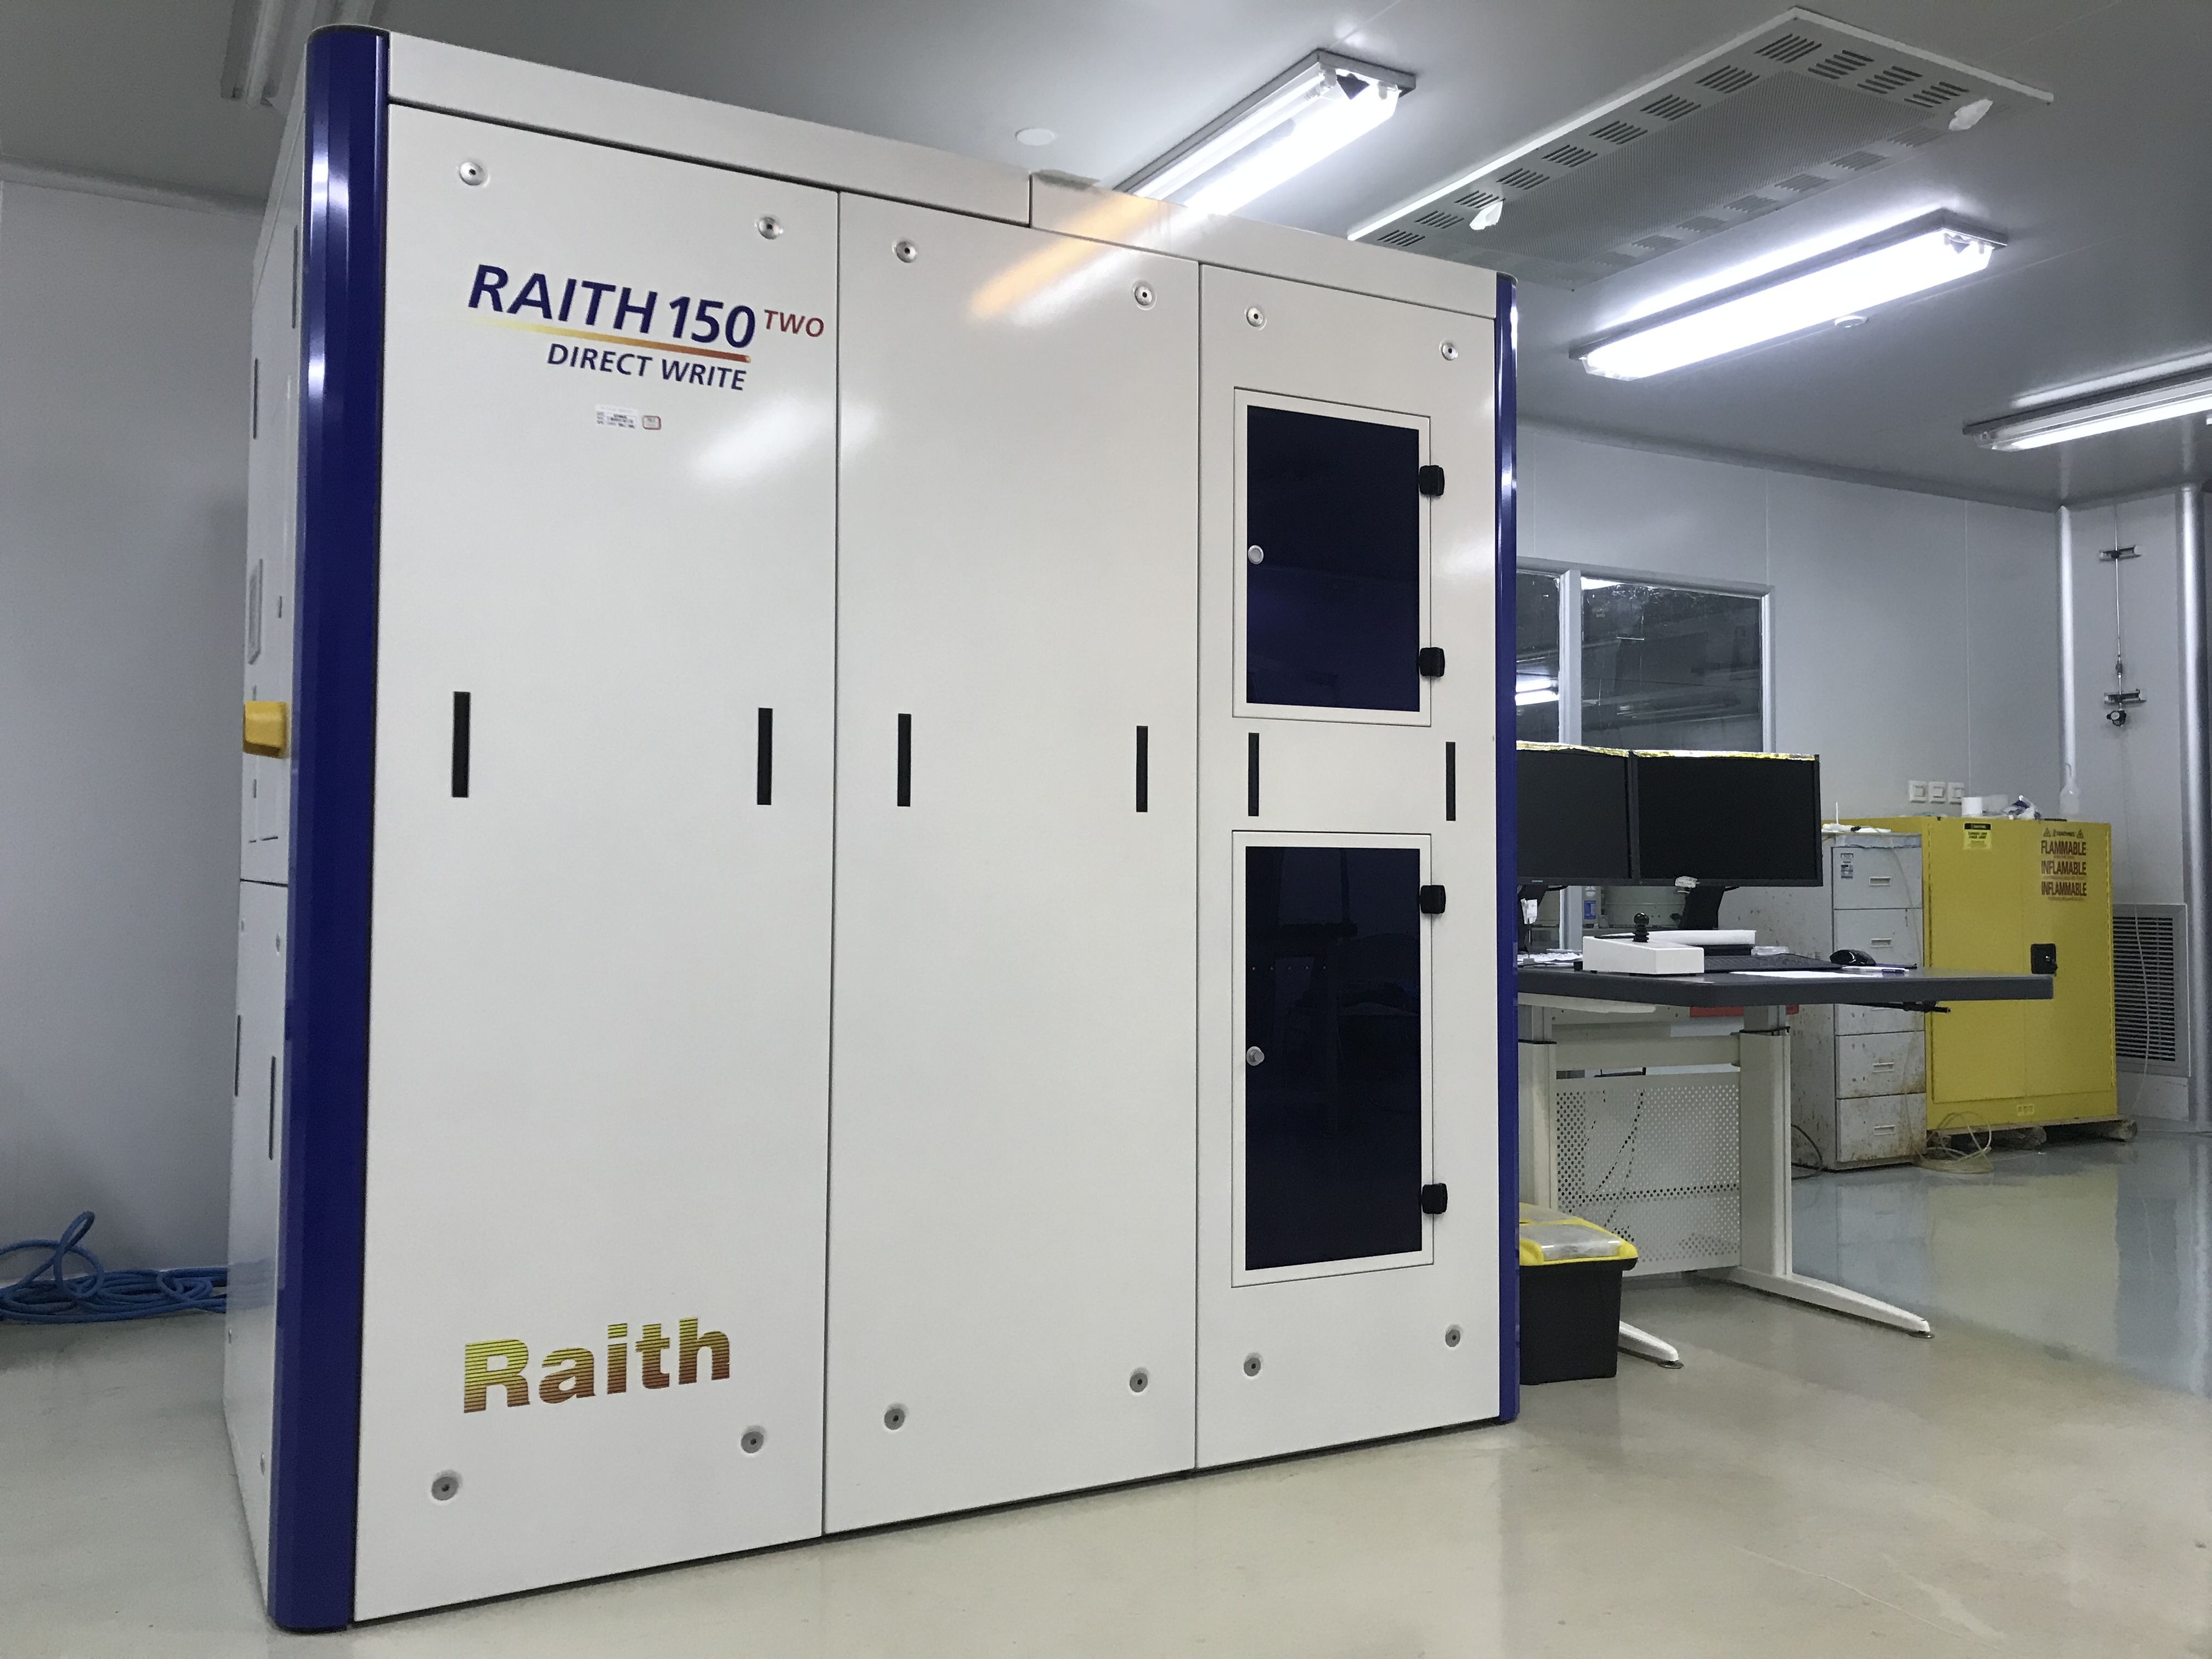
\includegraphics[width=12cm]{./Pictures/fab_ebl.jpg}
	\captionsetup{justification=centering}
	\caption{RAITH 150\SP{TWO}电子束曝光系统}
	\label{fab_ebl}
\end{figure}

我们以PMMA为例介绍电子束曝光过程中的注意事项,我们重点需要关注三个参数:加速电压、电子束光阑孔径和曝光剂量。加速电压主要决定了电子束能量的大小,加速电压越大,电子束的速度也会越大,在轰击样品表面时,越不容易发生大角度散射,故分辨率就会越高。本文后续实验所使用的Raith 150\SP{TWO}最大的加速电压为30~kV。电子束孔径主要控制曝光时电子束电流的大小,电子束孔径越大,则曝光时电子束的电流也就越大。对于同样的曝光图形,电子束孔径越大,曝光的时间就越短。但是电子束孔径增大时,对应的电子束发散程度也会变大,从而会降低分辨率。曝光剂量为单位面积内电子束光刻胶所需要的曝光电荷量,单位为$\mu C/cm^2$,主要由所用电子束光刻胶的性质和其成膜的厚度有关。以PMMA为例,若曝光剂量不足,则曝光区域的光刻胶在显影过程中就无法完全溶解,导致光刻胶的残留。若是曝光剂量过大,则会导致图形尺寸的展宽和侧壁粗糙度的增加。综上,电子束曝光过程的参数都要精心选择,以达到最好的曝光效果。

曝光完成之后,需要进行显影。对于PMMA来说,我们使用的显影液为MIBK(methyl isobutyl ketone) : IPA(isopropyl alcohol)=1:3(体积比)混合溶液,定影液采用IPA,显影参数为:显影35~$s$,定影35~$s$。然后用去离子水将显影液与定影液冲洗干净。

完成显影之后,我们需要对光刻胶进行坚膜处理,坚膜也称为后烘或者硬烘焙,它的作用是蒸发显影、定影过程中残留在基片表面的有机溶液,增强光刻胶与芯片表面的黏附力以及光刻胶的扛刻蚀性能。PMMA的坚膜过程如下:用热板60$^{\circ}$C烘烤5~$min$,再将热板温度设置到90~$^{\circ}$C并保持,继续烘烤几分钟,保证总的坚膜时间为15~$min$。坚膜完成之后,SOI芯片就可以进行后续的刻蚀工艺,将图案从光刻胶转移到芯片上。

\subsection{SOI芯片刻蚀工艺}

刻蚀工艺根据原理的不同,可以分为干法刻蚀与湿法刻蚀两大类。

湿法刻蚀不需要昂贵的设备,操作简单,是早期微纳加工过程中普遍采用的方法。湿法腐蚀硅较为常用的溶液一般有两种:一种是氢氟酸(HF)和硝酸(HNO\SB{3})的混合液,其与硅硅的化学反应式如下:
\begin{equation}
\rm Si+HNO_3+6HF\rightarrow H_2SiF_6+HNO_2+H_2O+H_2
\end{equation}
上式中的主要生成物H\SB{2}SiF\SB{6}与HNO\SB{2}均易溶于水,因此反应可以持续进行。但该方法的一个缺点是氢氟酸与衬底二氧化硅同样会发生反应。

另一种常用的腐蚀液为KOH溶液,其与硅的化学反应式如下:
\begin{equation}
\rm Si+2KOH+H_2O\rightarrow K_2SiO_3+2H_2
\end{equation}
需要特别指出的是,KOH溶液对于不同晶向的硅,其最终腐蚀得到的微槽结构也是不一样的。

湿法腐蚀的缺点在于腐蚀很难形成我们所需要的具有垂直侧壁的波导结构,其加工精度也有限,所以其应用范围也就受到了很大的局限。在对于刻蚀精度和刻蚀质量要求极高的硅基光电子集成器件中,已经极少使用湿法的方式来刻蚀波导器件结构。湿法刻蚀更多的是应用到某些特殊设计需要掏空的器件\cite{liu2016silicon}。

干法刻蚀是指利用化学或物理作用,或者两者同时作用的方法进行刻蚀。在纯化学机制中,主要通过受激等离子体产生的反应原子核自由基和被刻蚀物质之间的化学反应来完成刻蚀,刻蚀气体需要根据不同的刻蚀物材料来选择;在纯物理机制中,采用射频电源将刻蚀气体等离子体化,产生的等离子体高能粒子在电场作用下轰击刻蚀物质,该物理刻蚀方法具有很好的方向性,但缺点在于刻蚀的选择性较差。本文实验采用的是物理性的粒子轰击和化学反应刻蚀相结合的刻蚀方法,该方法又被称作电感耦合等离子体反应粒子刻蚀(Inductively Coupled Plasma Reactive Ion Etching, ICP-RIE)。图\ref{fab_icp}所示为本文所使用的英国STS公司的ICP刻蚀机。

\begin{figure}[htb]
	\centering
	\includegraphics[width=12cm]{./Pictures/fab_icp.jpg}
	\captionsetup{justification=centering}
	\caption{英国STS公司的ICP刻蚀机}
	\label{fab_icp}
\end{figure}

在ICP刻蚀过程中,物理轰击扮演了重要的角色。典型的ICP刻蚀过程包括刻蚀和淀积两类反应。反应物在刻蚀槽的底部和侧壁都会生成有机物保护层,由于等离子体向下轰击的方向性,使得底部的保护层比侧壁的保护层更快地被去掉,从而向下的刻蚀过程能持续进行,最终形成垂直的侧壁。在反应过程中,一般需要两种气体,一种作为刻蚀气体,另一种主要作为侧壁的保护气体。在刻蚀硅时,我们选用SF\SB{6}作为主要刻蚀气体,同时选用C\SB{4}F\SB{8}作为保护气体,合理调节两种气体的比例以及ICP的其他参数,可以使得刻蚀与淀积两种过程平衡,从而得到垂直的波导侧壁。本论文所使用的参数为:腔体温度65$^{\circ}$C,SF\SB{6}气体流量10~$sccm$,C\SB{4}F\SB{8}气体流量5.7~$sccm$,上极板功率为500~$W$,下极板功率为20~$W$,在该参数设定下,硅的刻蚀速率约为1.5~$nm$/s。

刻蚀工艺完成之后,我们需要去除残留的光刻胶和刻蚀残留物,以方便测试或者下一步工艺的顺利进行。去除残胶的常用的方式有如下三种:1、有机溶剂清洗;2、氧气等离子体轰击;3、强氧化剂比如食人鱼溶液清洗。有机溶剂一般采用的是丙酮或者强力去胶剂(N-Methy-Pyrrolidone, NMP),其一般可以溶解部分残胶,但是对刻蚀过程中已经碳化的光刻胶则无能为力。氧气等离子体则利用等离子态的氧气反应活性,与残胶发生氧化反应从而去除残胶。可以使用专门的氧气等离子体设备或者用ICP进行清洗。强氧化剂可以利用其强氧化特性,将残胶分解成CO、CO\SB{2}和H\SB{2}O,从而去除。实际工艺过程中,常常将这三种清洗方法组合使用。

\section{本章小结}
本章首先介绍了平板光波导的概念,并从麦克斯韦方程组出发推导了波动方程,并简要介绍了计算波导模式与光场传输的数值计算方法。然后介绍了DFB激光器的基本原理,包括其速率方程和耦合模理论,并利用速率方程计算得到了激光器的弛豫振荡频率,通过耦合模理论给出了DFB激光器单模激射的条件。最后介绍了本论文所用到的一些基本工艺流程,包括SOI芯片的清洗与匀胶,电子束曝光,刻蚀,并简要分析了其中的参数对工艺的影响。













\chapter{SOI刻蚀中的显色特性研究}
\section{背景介绍}

在SOI平台器件加工的过程中,标准SOI的硅层厚度通常只有几个固定的值,比如220~$nm$,340~$nm$,如图\ref{color_wafer}所示。图\ref{color_wafer}(a)所示为硅层厚度220~$nm$的12英寸SOI芯片,其颜色显示为淡绿色,但由于硅层厚度的不均匀性,中间与边缘区域表现为淡紫色。图\ref{color_wafer}(b)所示为硅层厚度340~$nm$的12英寸SOI芯片,其颜色显示为淡紫色,但由于硅层厚度的不均匀性,边缘区域表现为淡绿色。上述颜色均为日光灯下接近垂直视角所拍摄的颜色。

\begin{figure}[htb]
	\centering
	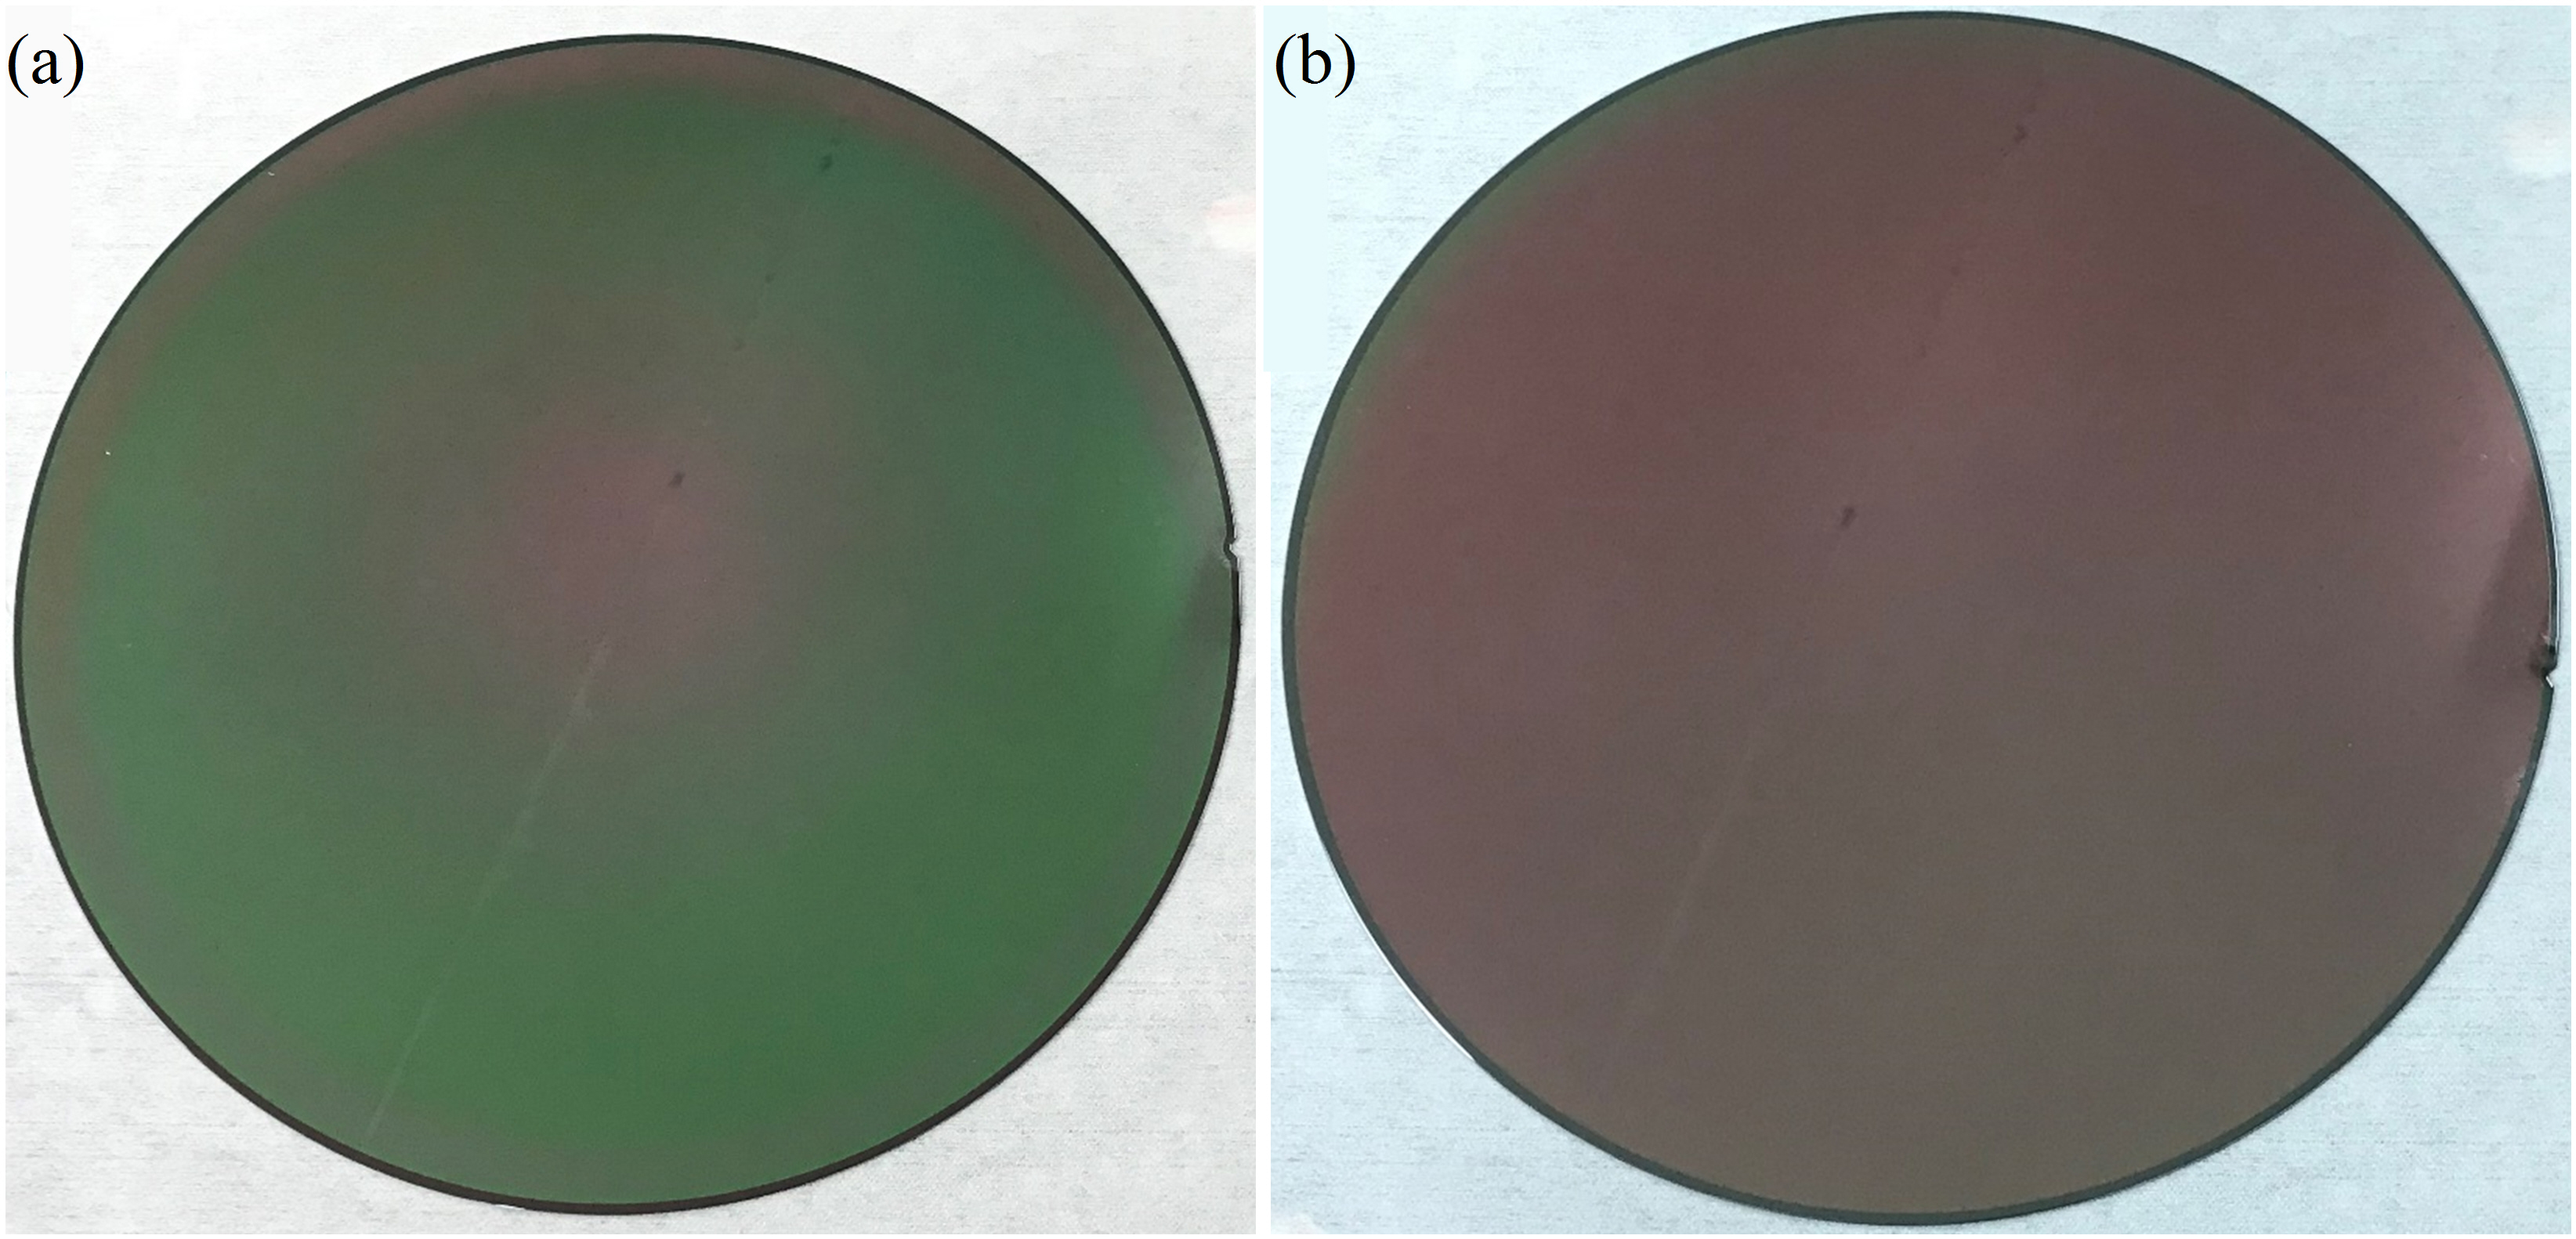
\includegraphics[width=14cm]{./Pictures/color_wafer.jpg}
	\captionsetup{justification=centering}
	\caption{标准12英寸SOI芯片,(a)~220~$nm$硅层厚度;(b)~340~$nm$硅层厚度}
	\label{color_wafer}
\end{figure}

传统的硅波导的厚度大约在200~\~{}500~$nm$之间,近年来人们开始研究超薄硅波导,其相较于220~$nm$厚的传统硅波导来说,有以下几种优势:首先,因为超薄硅波导中的模式相对于传统波导中的模式对侧壁粗糙度更加不敏感,所以其传输损耗相比于传统220~$nm$厚的硅波导来说可以降低,Dumon等人测得对于高度为220~$nm$的硅波导,当波导宽度分别为400~$nm$、450~$nm$和500~$nm$时,其在1550~$nm$对应的损耗分别为33.8~dB/$cm$、7.4~dB/$cm$和2.4~dB/$cm$\cite{dumon2004low},Zou等人制作的高度为60~$nm$,宽度为950~$nm$的硅波导,损耗降到了0.61~dB/$cm$\cite{zou201560}。其次,由于超薄硅波导对光的限制能力变弱,等效折射率会降低,使得器件特征尺寸可以相对增大,更容易用较低成本的光刻技术加工\cite{zou201560}。超薄硅波导满足单模条件的波导宽度的也会更宽,且当波导宽度越大的时候,等效折射率对波导宽度的变化率就会降低,故超薄硅波导的制作容差就会变大。还有,对于模式转换器件来说,超薄硅波导的模式限制较弱,这意味着模式之间的重叠会增多,更容易实现超短的转换结构。在传感领域,由于超薄硅波导的模式限制较弱,故可以增强光场与物质的相互作用,从而提高器件的灵敏度。最后,由于超薄硅波导的宽高比很大,故可以减轻刻蚀过程中的迟滞效应\cite{jansen1997bsm},更容易制作波导之间的缝隙,并且该缝隙也更容易用二氧化硅等包层材料进行填充。

\begin{figure}[htb]
	\centering
	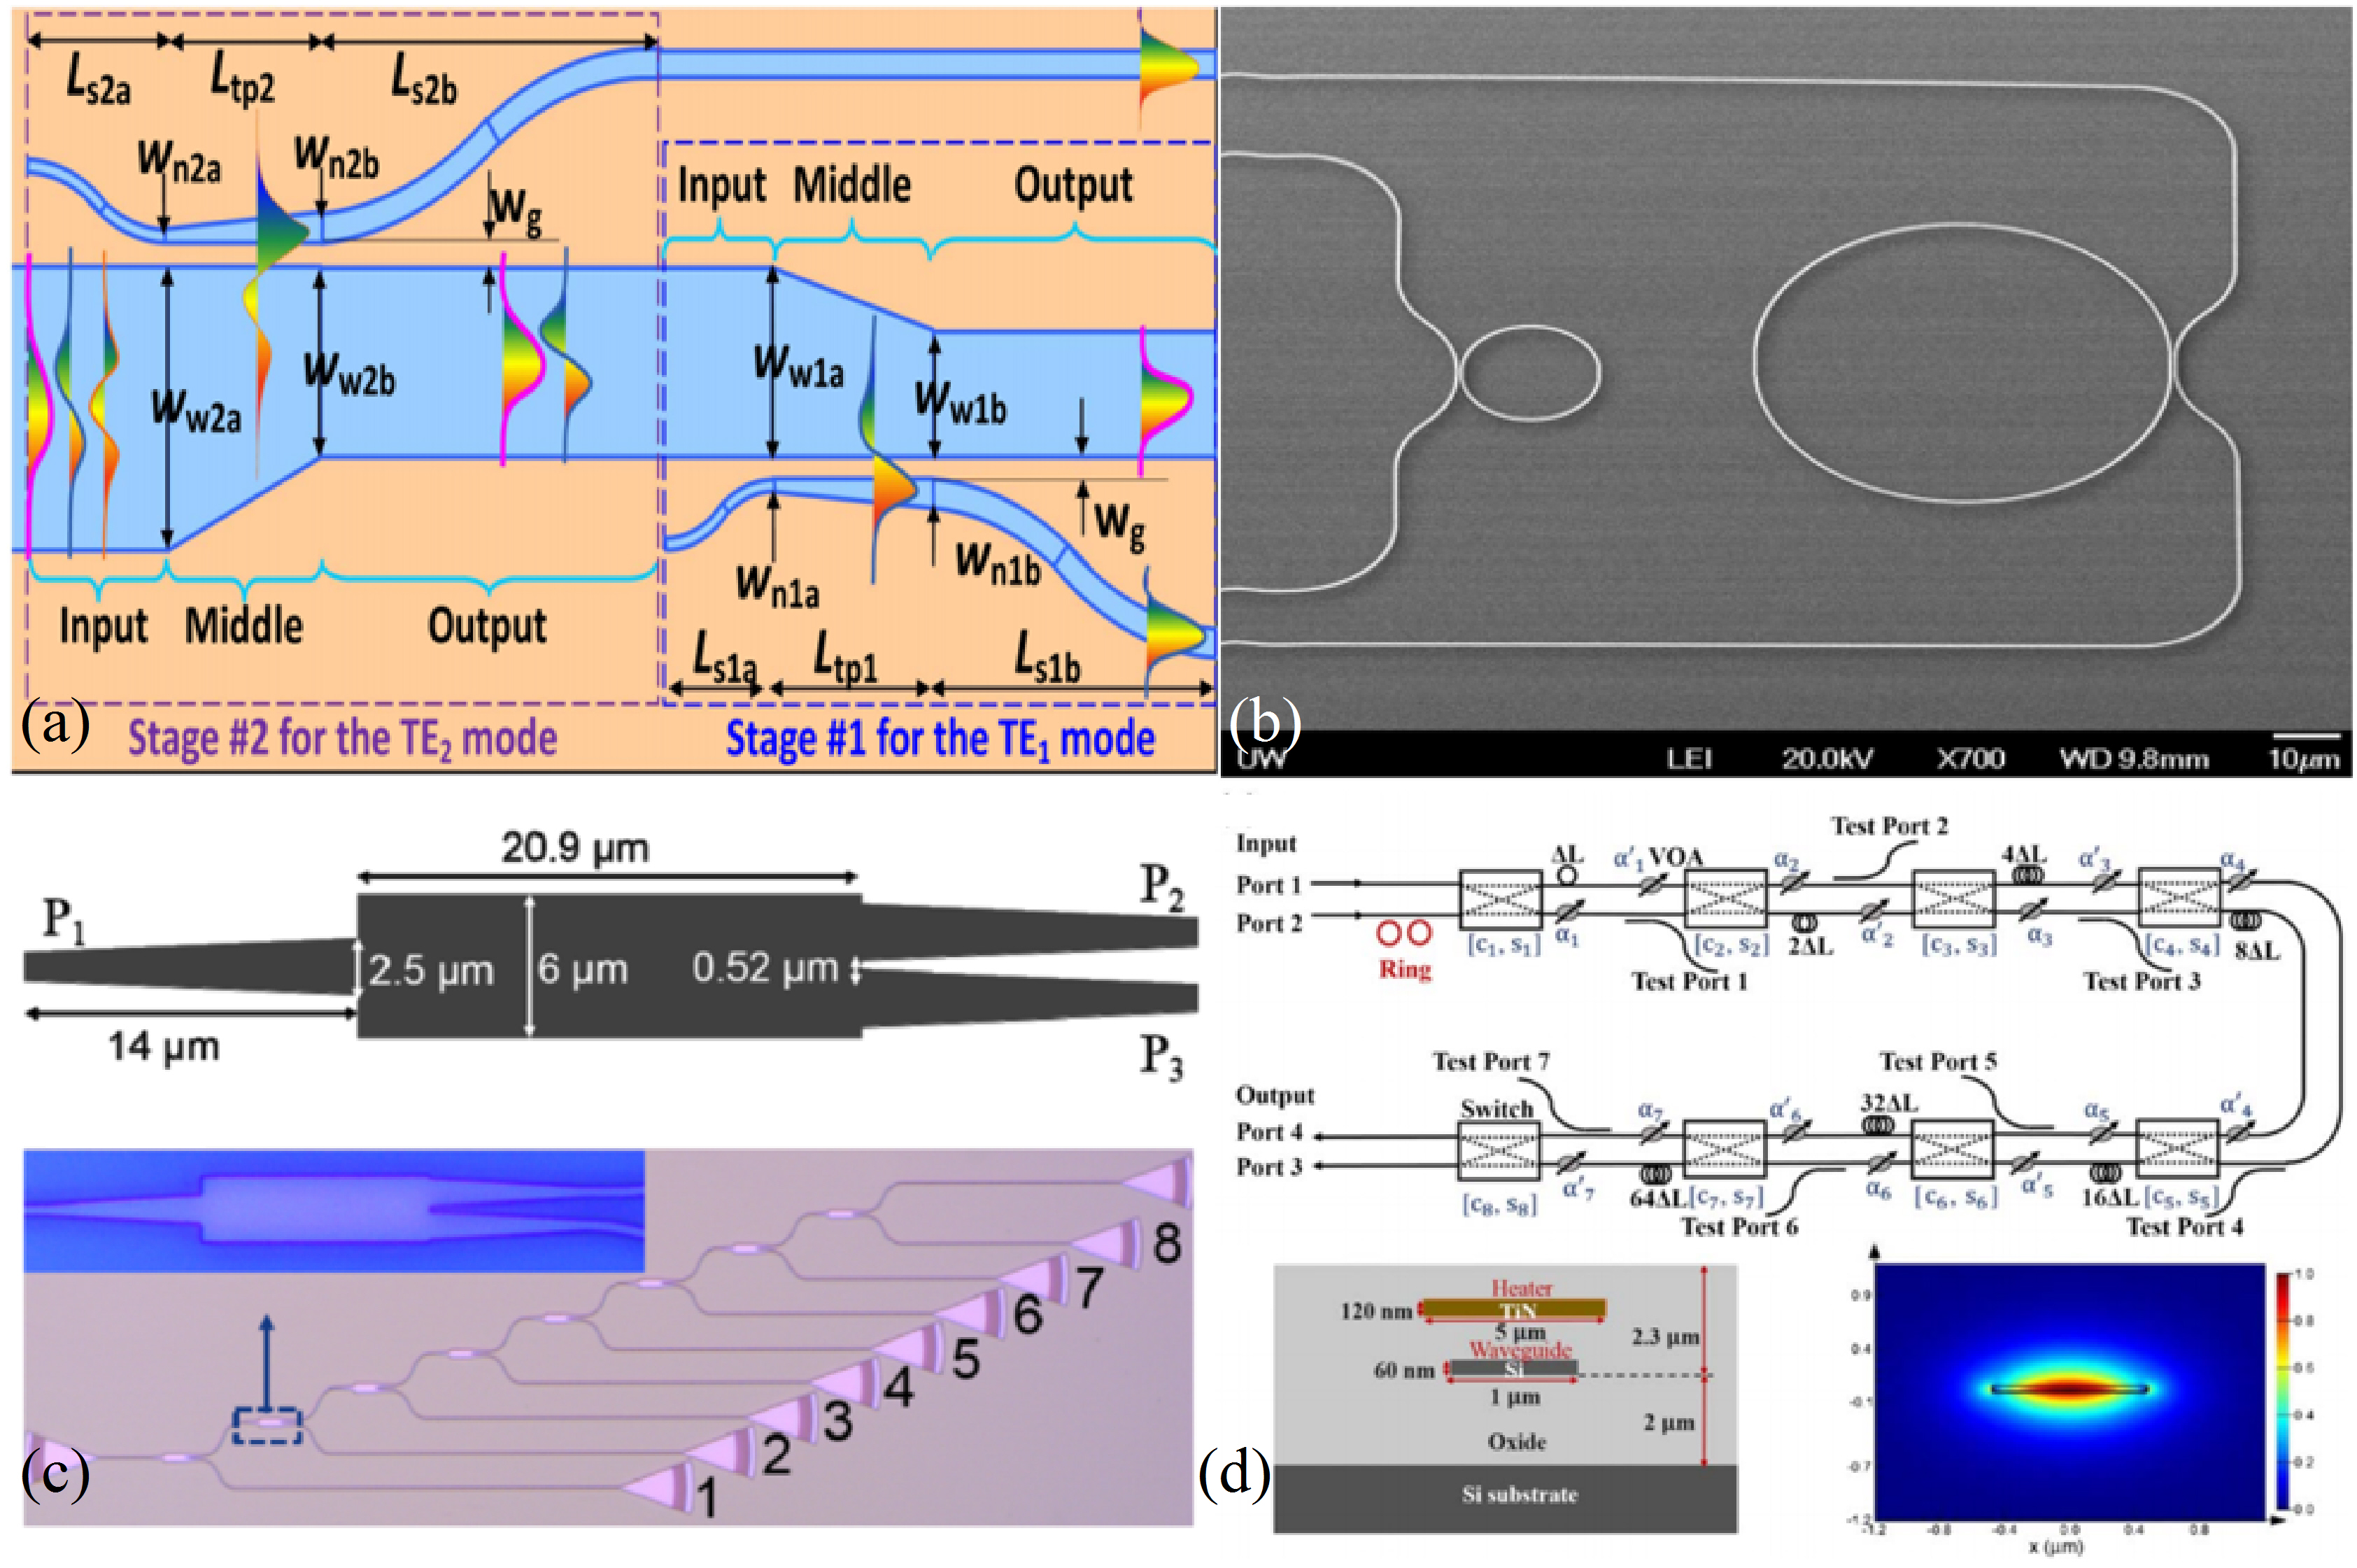
\includegraphics[width=14cm]{./Pictures/color_thin_application.jpg}
	\captionsetup{justification=centering}
	\caption{超薄硅器件,(a)模分复用解复用器,硅层厚度为50~$nm$\cite{li2017low};(b)微环传感器,硅层厚度为90~$nm$\cite{fard2014performance};(c)多模干涉耦合器,硅层厚度为60~$nm$\cite{zou201560};(d)延时线,硅层厚度为60~$nm$\cite{wang2017continuously}}
	\label{color_thin_application}
\end{figure}

利用超薄硅波导,Li等人制作了一个模分复用解复用器\cite{li2017low},如图\ref{color_thin_application}(a)所示,硅层厚度为50~$nm$,得益于超薄硅波导的低损耗,易耦合且制作容差大的优点,该模分复用解复用器在理论上可以实现在200~$nm$带宽范围内插损小于0.2~dB,在130~$nm$带宽范围内串扰小于-20~dB。当制作容差达到20~$nm$时,损耗基本不变,在大于100~$nm$带宽范围内依然能够保持串扰小于-20~dB;Fard等人利用超薄硅制作了微环传感器\cite{fard2014performance},如图\ref{color_thin_application}(b)所示,硅层厚度为90~$nm$,利用超薄硅波导模式体积大的优势,该器件实现了TE模式超过100~$nm$/RIU的灵敏度,比传统硅波导制作的微环传感器要高,而且相比于传统的220~$nm$硅层厚度的微环谐振腔,该器件的热稳定性也更好;Zou等人利用60~$nm$厚度的硅波导制作了一分二的多模干涉耦合器(Multimode Interfenrence coupler, MMI coupler)\cite{zou201560},如图\ref{color_thin_application}(c)所示,实验测得该多模干涉耦合器在1535~$nm$\~{}1587~$nm$波长范围内6插损小于0.2~dB;Wang等人也在60~$nm$厚的硅波导平台上利用微环和级联开关阵列制作了延时线\cite{wang2017continuously},如图\ref{color_thin_application}(d)所示,其波导平均损耗为0.35~dB/$cm$,时延的最大调节值为1.28~$ns$。

为了获得超薄硅,人们通常是将现有的SOI芯片做减薄处理以得到所需要的厚度。首先想到的是利用湿法腐蚀对硅层厚度进行减薄,但是由于硅的晶格结构,使其湿法腐蚀具有各向异性,如图\ref{color_silicon_crystal}所示。对于表面为\{111\}晶面的SOI芯片,由于其晶格结构较为致密,故很难用碱性溶液进行腐蚀;对于表面为\{100\}晶面的SOI芯片,用碱性腐蚀液腐蚀会形成金字塔结构,其侧边四个面为较难腐蚀的\{111\}面,利用该特性,可以在制作单晶硅太阳能电池时减小反射,增加光的吸收效率;对于表面为\{100\}晶面的SOI芯片,用碱性腐蚀液会形成垂直的沟槽,沟槽的侧面为较难腐蚀的\{111\}面,利用该特性可以用来制作微流通道。

\begin{figure}[htb]
	\centering
	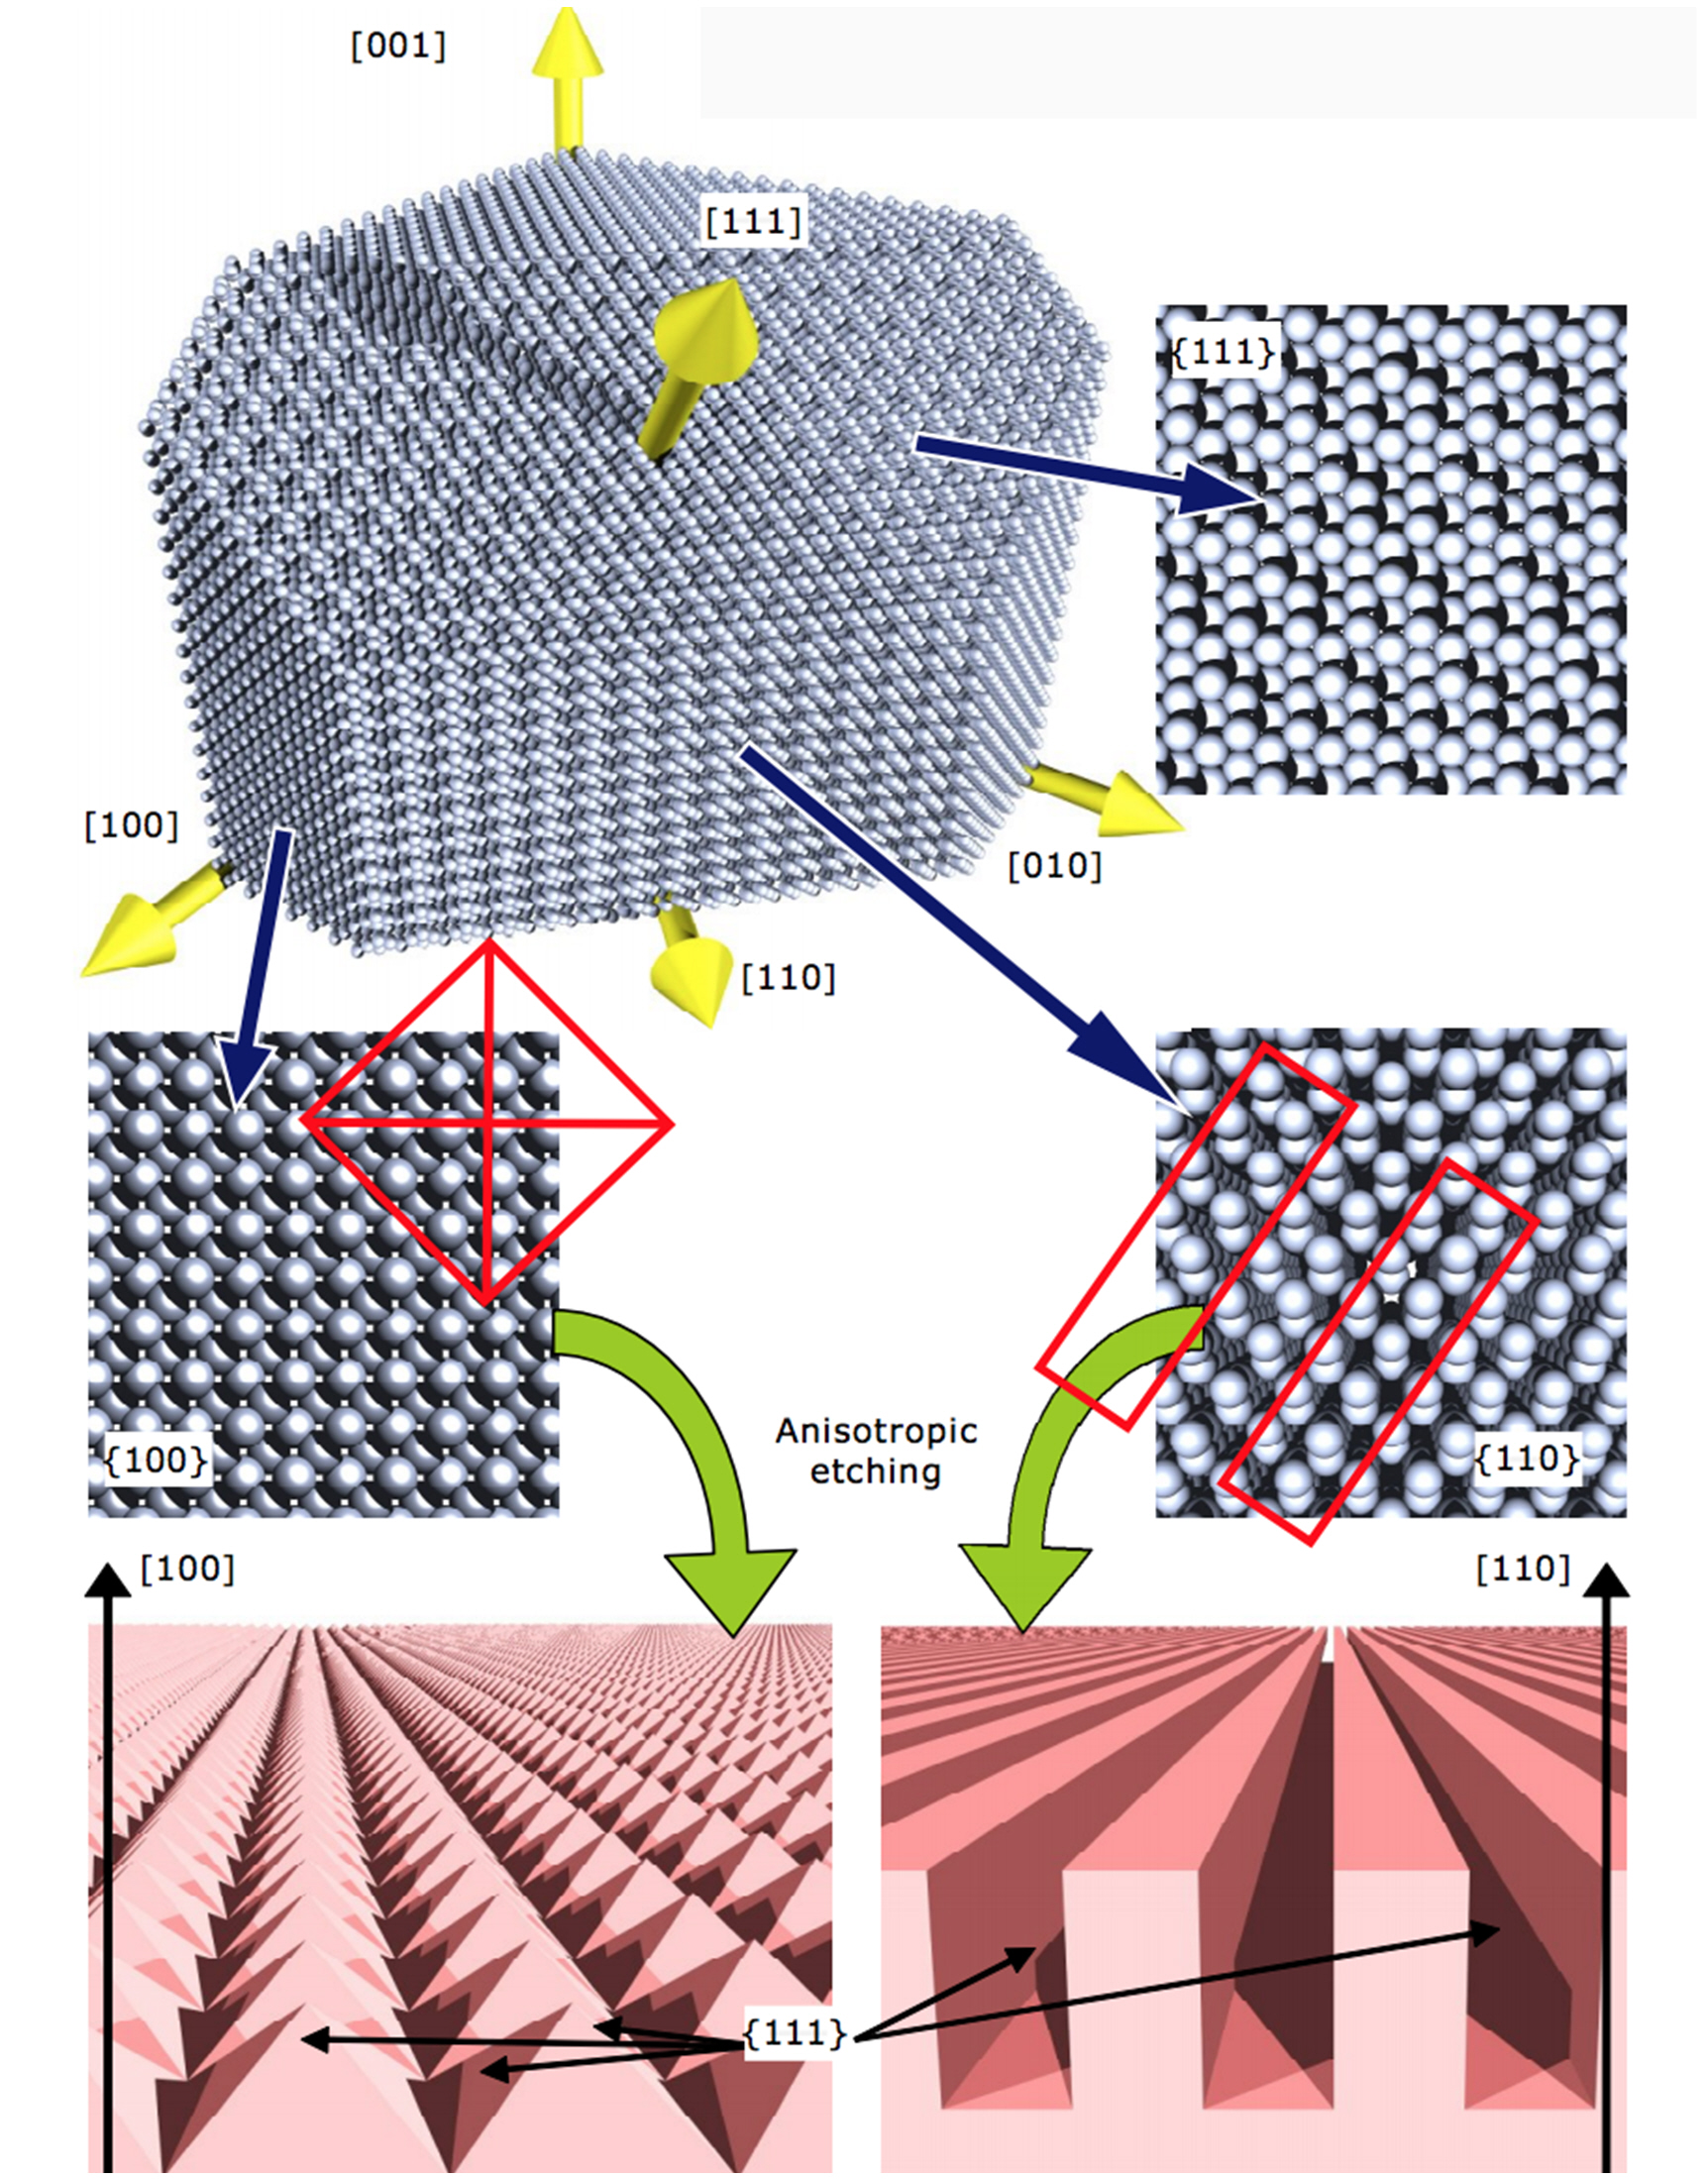
\includegraphics[width=12cm]{./Pictures/color_silicon_crystal.jpg}
	\captionsetup{justification=centering}
	\caption{硅的晶格结构及湿法腐蚀特性\cite{microchemicals}}
	\label{color_silicon_crystal}
\end{figure}

由于湿法腐蚀无法对SOI芯片均匀减薄,通常用来对SOI芯片减薄的方法有两种,一种是用ICP对较厚的SOI芯片进行刻蚀,这种方法的优势是工艺方便,缺点是表面会比较粗糙且厚度不均匀,会影响器件的损耗等性能,Zou等人采用该方法来减薄220~$nm$~SOI芯片得到60~$nm$厚的硅波导,损耗为0.61~dB/$cm$\cite{zou201560}。另一种方法是用热氧的方法氧化表面硅层之后用HF溶液去除氧化层,使得SOI芯片的硅层厚度减薄,Wang等人利用热氧化的方法制作了60~$nm$厚的硅波导,其波导损耗可以减小到0.35~dB/$cm$\cite{wang2017continuously}。相比较而言,利用热氧法进行硅层的减薄可以得到更低的损耗。

除了如图\ref{color_thin_application}中所示的一些器件需要将标准SOI芯片减薄,在许多常用硅基光电子器件制作测试时,我们也经常需要制作浅刻蚀的光栅耦合器方便器件的测试\cite{taillaert2004compact}。由于实验室的设备因为稳定性的原因,如果每次都通过制作测试片再用划台阶仪的方法来确定刻蚀速率或者氧化速率,则会增加工艺步骤,比较费时费力。这时如果有一种能够帮助我们快速确定薄硅层厚度的方法,就能给器件的工艺制作提供极大的便利。我们通过平时实验的经验发现,不同的刻蚀深度对应的SOI芯片颜色会有所不同。如图\ref{color_etch_time}所示,可以看到SOI芯片经过不同时间的ICP刻蚀,所剩下的不同厚度硅层显示出来的颜色信息非常丰富,硅层厚度为220~$nm$的SOI芯片没有刻蚀前显示为淡绿色,通过不同时间的刻蚀,会显示出紫色、黄色、蓝色等丰富的颜色,故我们对其进行了较为深入的研究,以期找出硅层厚度与颜色的对应关系。

\begin{figure}[htb]
	\centering
	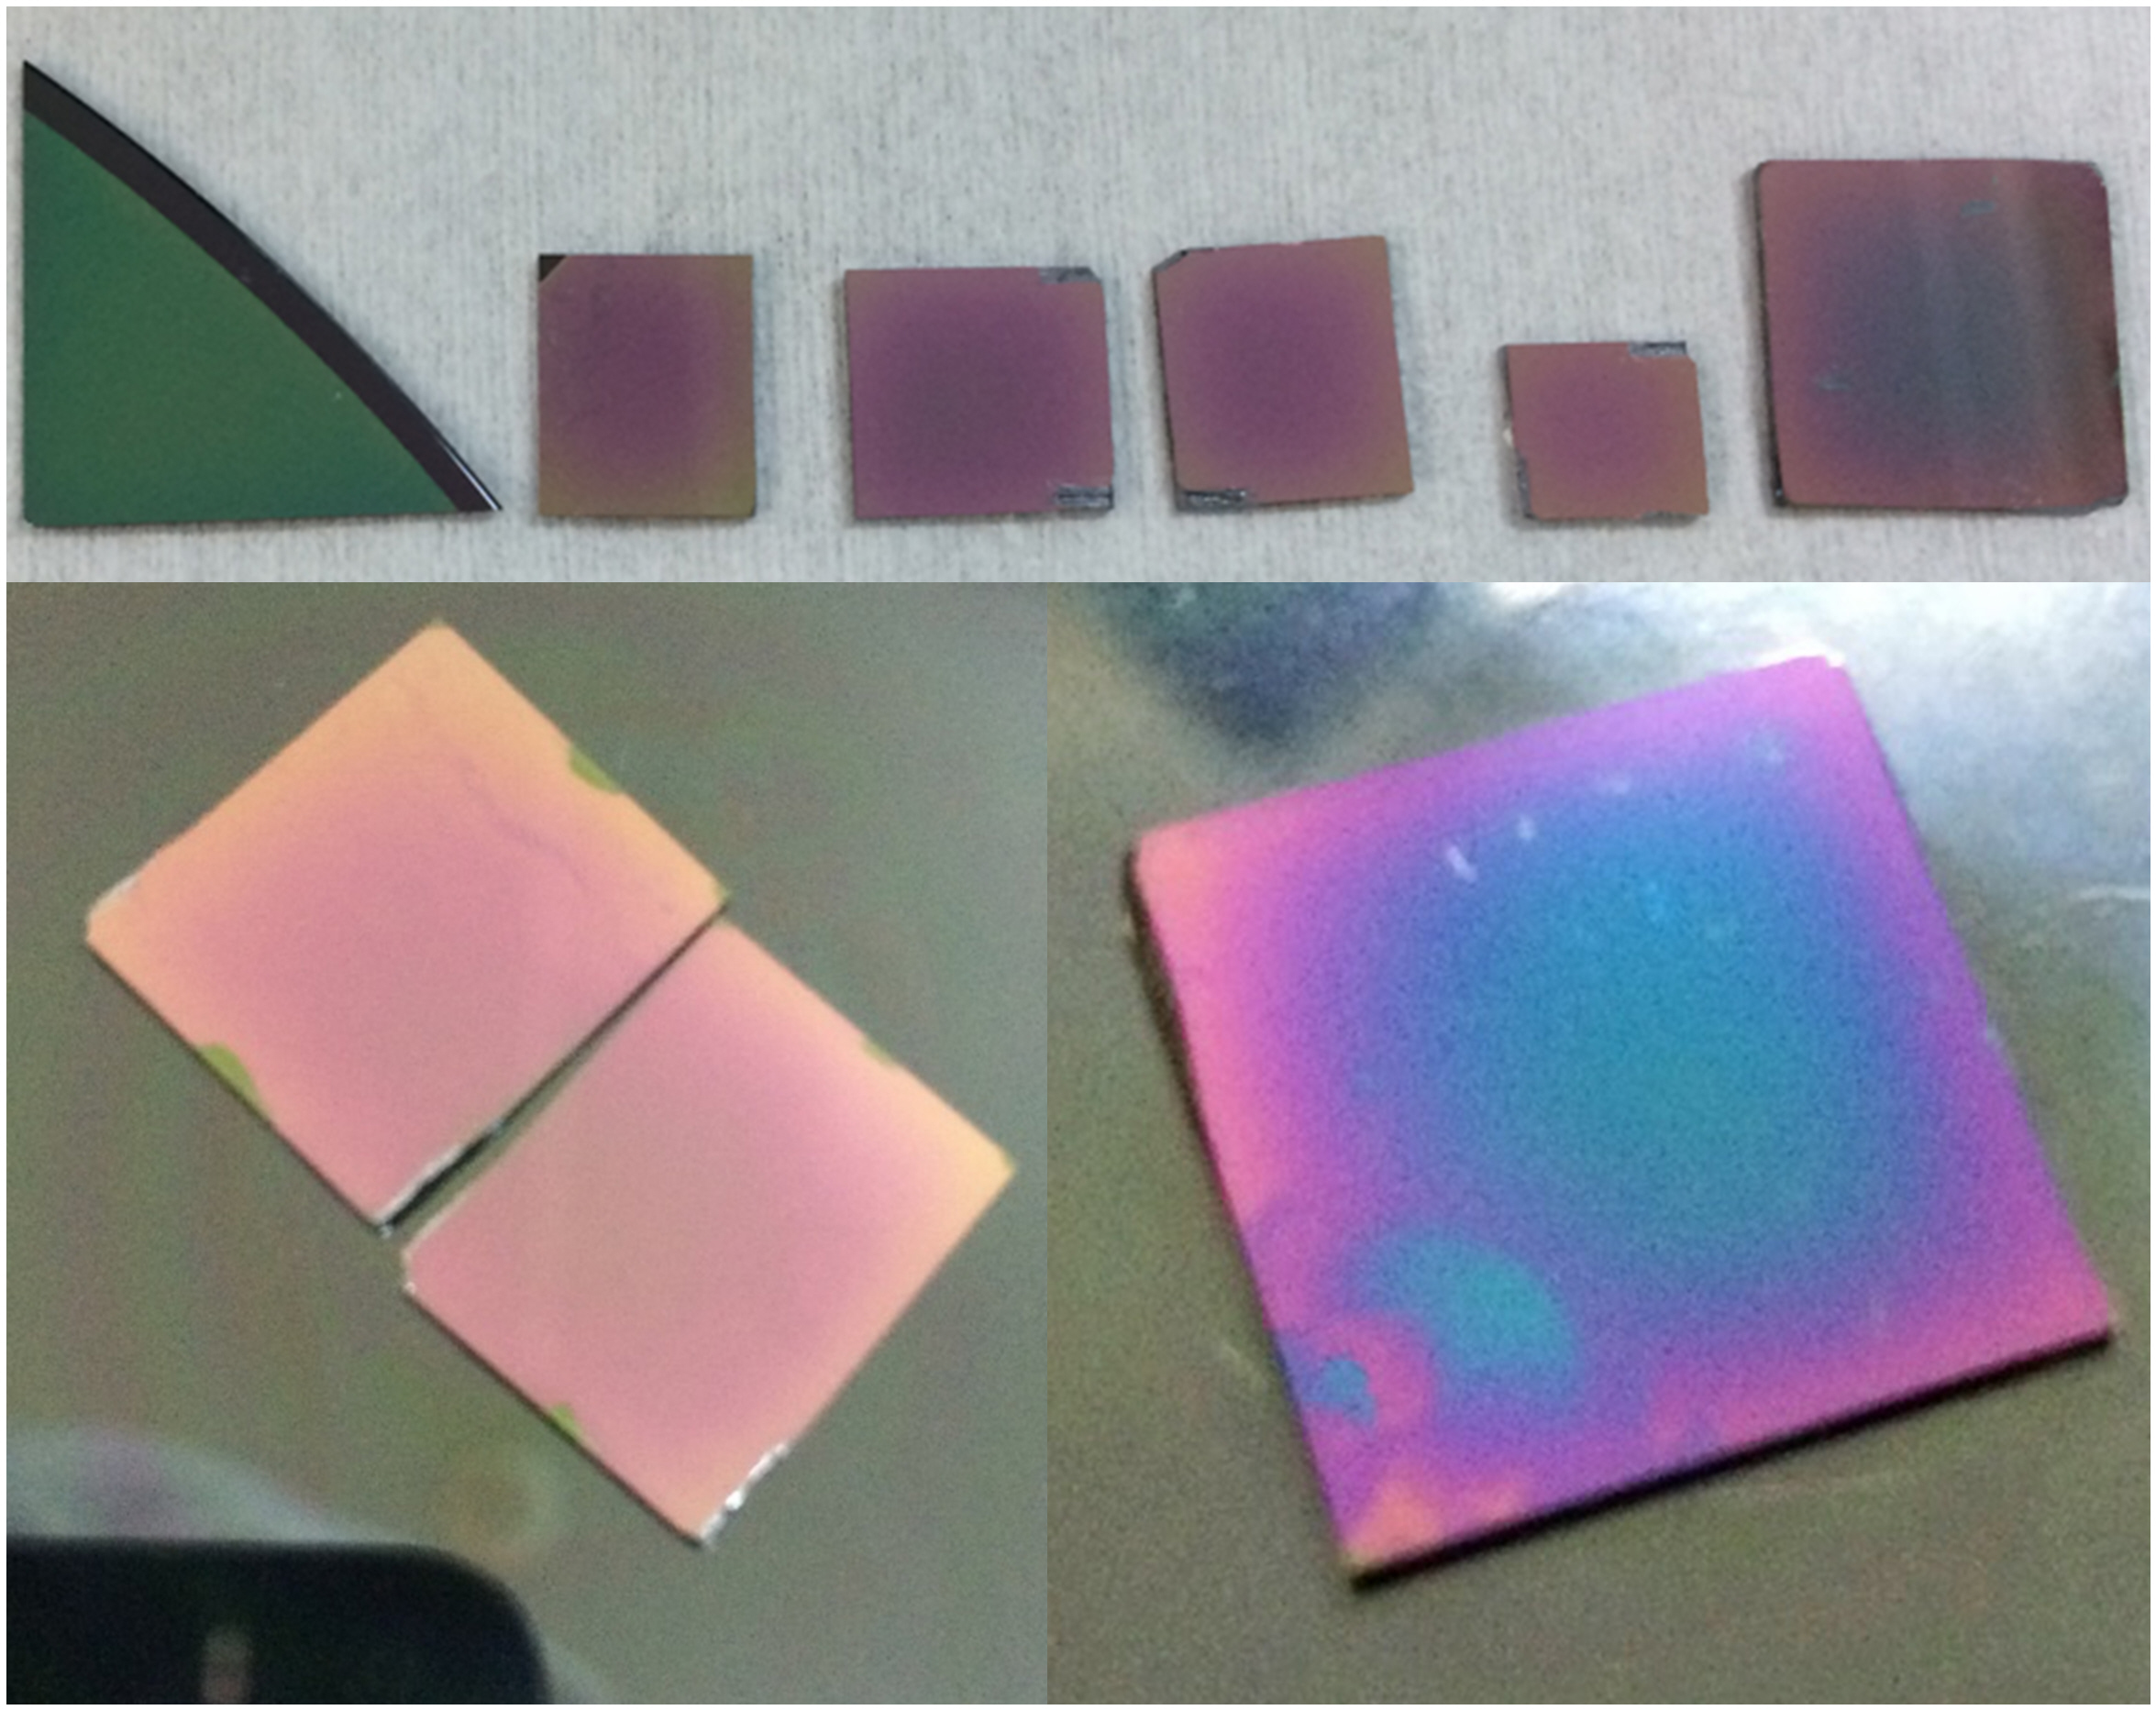
\includegraphics[width=12cm]{./Pictures/color_etch_time.jpg}
	\captionsetup{justification=centering}
	\caption{不同刻蚀深度对应的SOI的颜色}
	\label{color_etch_time}
\end{figure}

\section{光度学与色度学基础}
为了研究跟颜色相关的问题,我们首先需要一些光度学与色度学的基础。光是一种电磁波,其波长范围覆盖从1~$nm$以下直到10\SP{3}~$km$,其辐射类型按能量从高到低包括$\gamma$射线、X射线、紫外线、可见光、红外线、微波、无线电等。在整个电磁波谱中,只有很小的一部分进入人眼之后能引起我们的视觉感知,这部分光辐射谱被称为可见光谱,简称可见光。一般认为可见光的波长范围在380~$nm$\~{}780~$nm$之间,我们人眼所能够感知到的颜色都只与这个波长范围内的电磁波有关。不同波长的可见光辐射进入人眼,引起不同的颜色感觉,单一波长的可见光表现为一种颜色,称为单色光或者光谱色。

除了激光之外,日常生活中见到单色光的机会并不多,一般接触到的都是复色光。复色光中不同波长的单色光的相对功率分布决定了我们对它的颜色感觉。所以,成分确定的复色光一定对应一种确定的颜色。但是,一种确定的颜色并不只对应一种光谱组合,即两种不同的成分组合的复色光可以引起我们相同的颜色感觉,这在颜色科学中就是很重要的同色异谱问题。在我们之后的研究中也可以发现,不同硅层厚度可能对应相同的颜色。

要确定一个物体的颜色,我们就需要确定该物体在可见光波段所发射的光谱。如果该物体是光源,那么我们只需要知道该光源的发射谱;如果该物体本身并不发光,我们就需要确定光源的光谱,以及该物体对不同波长的光的反射率或者透射率,从而确定我们观察到该物体的光谱,之后就能确定该物体的颜色。

可见光在380~$nm$\~{}780~$nm$波长范围内的电磁辐射能量,可以用辐射量来描述,但是可见光对人的视觉形成刺激的程度不仅与电磁辐射的能量有关,还与人眼的响应有关,故我们需要用光学量(光度量)来描述其强弱。人们把定量地测定光的明亮程度的科学称为光度学(photometry)。辐射量是单位为焦耳($J$),瓦特($W$)等的物理量,而光学量是由视觉心理来评价物理量时得到的量,称为心理物理量,单位为流明($lm$),勒克斯($lx$)等。由此可见,当把可见光当做纯物理现象来研究时,应采用辐射量量值系统;当研究与人的视觉有关问题时,应采用光学量量值系统。为了后面讨论的方便,我们有必要介绍部分辐射量与光学量,以及两种量值之间的关系\cite{ydy2011gcgx,lxt2007jhgx}。

\subsection{辐射量}

\begin{enumerate}[(1)]
	\item
	辐射能$Q_{e}$~~~~同其他电磁辐射一样,可见光辐射也是一种能量传播形式。以电磁辐射形式发射、传输或接收的能量称为辐射能,通常用字符$Q_{e}$表示。度量辐射能的单位为焦[耳]($J$)。
	\item 
	辐射能通量$\Phi_{e}$~~~~单位时间内发射、传输或接收辐射能称之为辐射能通量,通常用字符$\Phi_{e}$表示。若在$dt$时间内发射、传输或接收的辐射能为d$Q_{e}$,相应的辐射能通量$\Phi_{e}$为:
	\begin{equation}
	\label{radiation_rate}
	\Phi_{e} = \dfrac{dQ_{e}}{dt}
	\end{equation}
	辐射能通量与功率有相同的单位,为瓦特($W$)。
	
\end{enumerate}
其他更多的辐射量由于跟本章内容无关,我们不再进行介绍。

\subsection{光学量}
\begin{enumerate}[]
	\item 
	光通量$\Phi_{v}$~~~~标度可见光对人眼的视觉刺激程度的量称为光通量,通常以字符$\Phi_{v}$表示。光通量的单位为流明($lm$)。
\end{enumerate}

其他更多的光学量量由于跟本章内容无关,我们不再进行介绍。

\begin{comment}
\begin{figure}[htb]
	\centering
	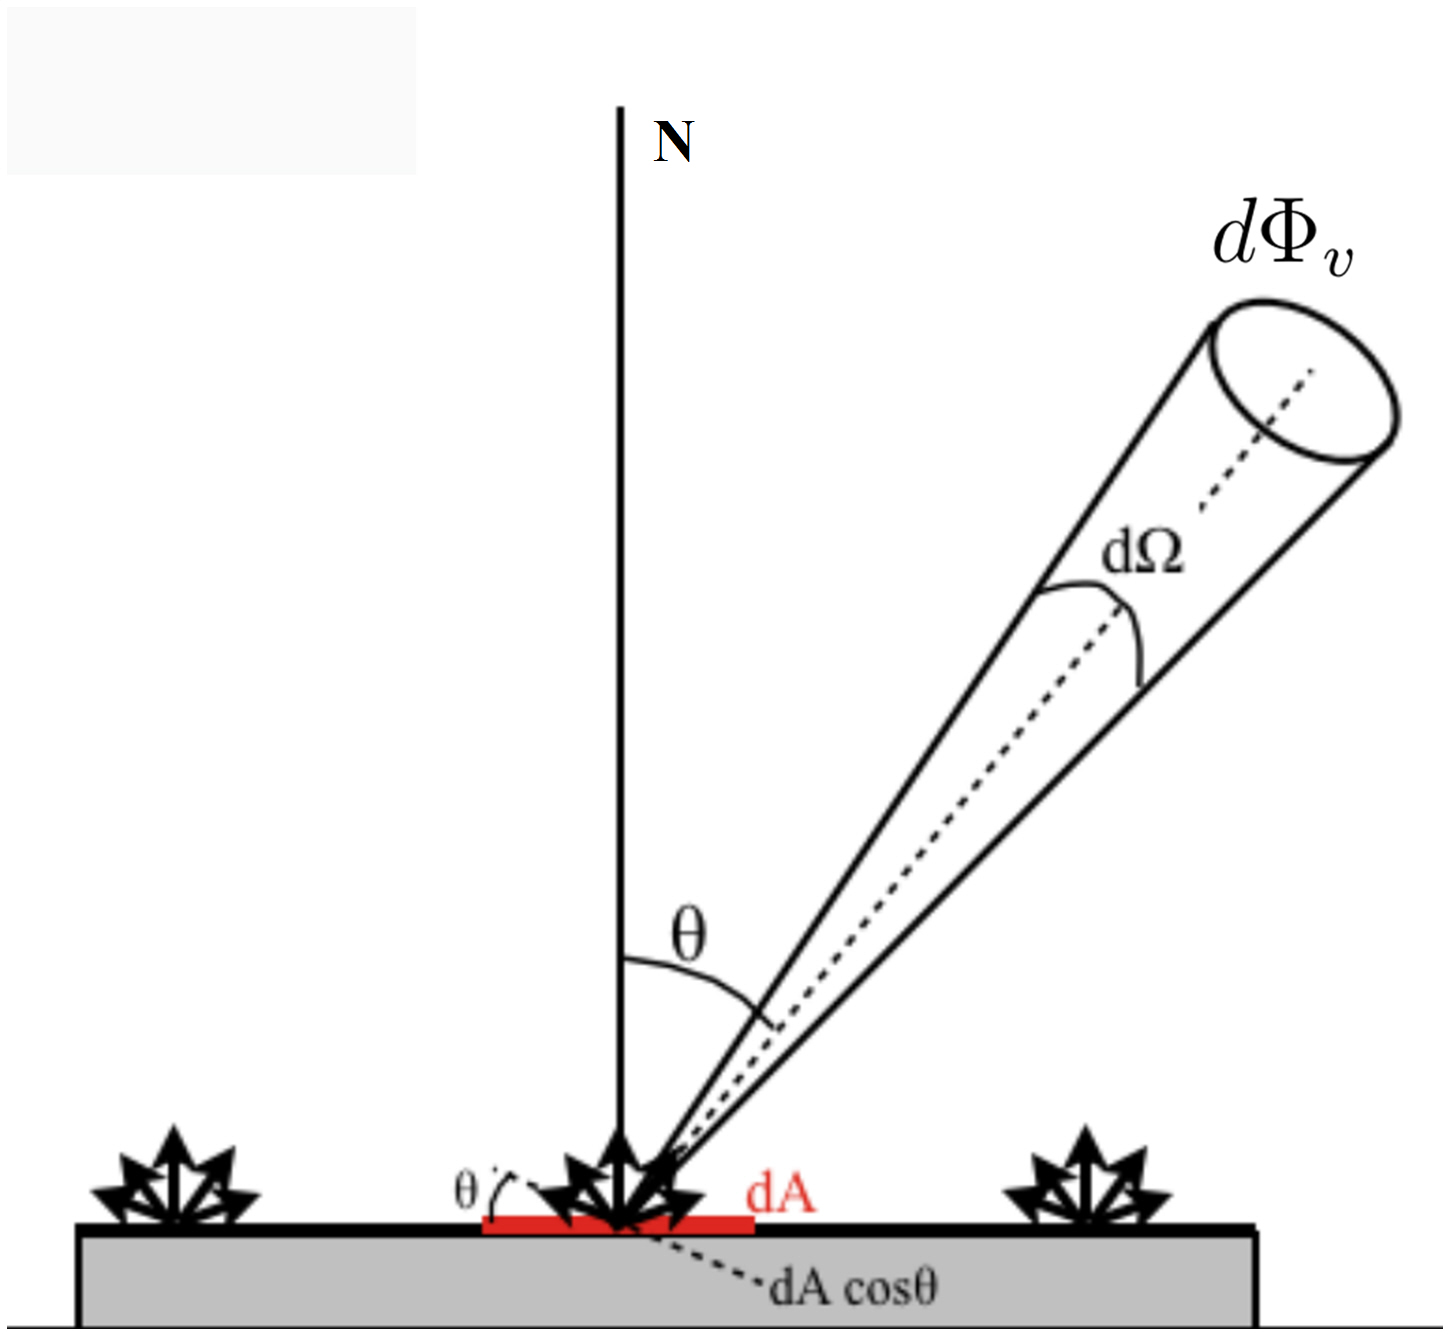
\includegraphics[width=12cm]{./Pictures/color_brightness.jpg}
	\captionsetup{justification=centering}
	\caption{光亮度定义示意图\cite{yalebrightness}}
	\label{color_brightness}
\end{figure}
\end{comment}

\subsection{光学量与辐射量之间的关系}
人的眼睛具有正确比较两个光刺激的强弱和判断其是否相等的能力,这是光度学的基础。但人眼对不同波长单色光的敏感程度并不一样,即相同功率的不同单色光所引起的光通量是不相同的。经过大量的实验确定,人眼对波长为555~$nm$的黄色光最为敏感,这正好是太阳辐射能量最高的波长附近。如果在单位波长内$P_{\lambda}$瓦的辐射能通量相当于$\Phi_{\lambda}$流明的光通量,则其比值:
\begin{equation}
\label{luminance_per_watt}
K_{\lambda} = \dfrac{\Phi_{\lambda}}{P_{\lambda}}
\end{equation}
可表示1瓦辐射能通量能量所相当的流明数。因为人眼对555~$nm$波长的黄光最为敏感,所以此数值在波长等于555~$nm$时取得最大。任一其他波长的单色光的$K_{\lambda}$值与$K_{555}$之比表征了人眼对该单色光辐射的相对灵敏度,称为光谱光视效率(spectral luminous efficiency)或视见函数(visibility function),以$V_{\lambda}$表示,即:
\begin{equation}
\label{visibility_function}
V_{\lambda} = \dfrac{K_{\lambda}}{K_{555}}
\end{equation}

\begin{figure}[htb]
	\centering
	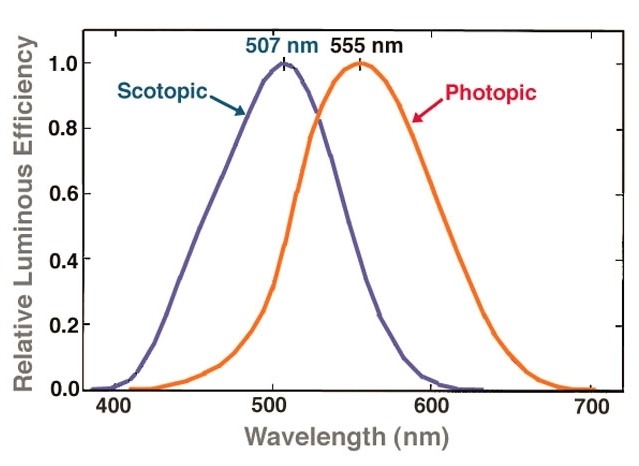
\includegraphics[width=11cm]{./Pictures/color_luminous_efficiency.jpg}
	\captionsetup{justification=centering}
	\caption{明场与暗场下相对光谱光视效率函数\cite{webvision}}
	\label{color_luminous_efficiency}
\end{figure}

不同波长单色光的光谱光视效率值是在做大量实验的基础上,由国际照明委员会(Commission Internationale de l´Eclairage, CIE)所确定的。实验表明,观察场明暗不同时,光谱光视效率亦稍有不同,这是由于人眼中的感光细胞分为视锥细胞和视杆细胞,视锥细胞工作在明视觉的情况下,可以感知颜色,但是灵敏度不如视杆细胞;视杆细胞工作在暗视觉的情况下,不能感知颜色,但是灵敏度很高。因此光谱光视效率函数在明暗场时略有不同,如图\ref{color_luminous_efficiency}所示,图中黄色曲线代表明场条件下的光谱光视效率函数,在555~$nm$处取得最大值,紫色曲线代表暗场(照度小于0.1~$lx$)\cite{hunt1995reproduction}条件下的光谱光视效率函数,在507~$nm$处取得最大值。在研究SOI芯片的硅层厚度与其颜色之间的对应关系时,我们只考虑明场的情况。

在波长$\lambda$附近的小波长间隔d$\lambda$内,光通量d$\Phi_{v}(\lambda)$和辐射能通量d$\Phi_{e}(\lambda)$之间的关系可以表示为:
\begin{equation}
\label{relation1}
d\Phi_{v}(\lambda)~=~K_{m}V(\lambda)\Phi_{e}(\lambda)d\lambda
\end{equation}
其中,$K_{m}$ = 683 $lm$/W为明视觉条件下波长为555~nm单色光的绝对光谱光视效率值;$K_{m}^{,}$ = 1755 lm/W为暗视觉条件下波长507~$nm$单色光的绝对光谱光视效率值。对于整个可见光谱范围内的总光通量$\Phi_{v}$,可由公式\ref{relation1}积分得到:
\begin{equation}
\label{relation3}
\Phi_{v}(\lambda)~=~\int_{380}^{780}K_{m}V(\lambda)\Phi_{e}(\lambda)d\lambda
\end{equation}

\subsection{CIE1931-RGB系统}
人们做了大量的颜色匹配实验,得出如下两个结论:
\begin{enumerate}[(1)]
	\item 
	红、绿、蓝三种颜色以不同的量值(有的可能为负值)相混合,可以匹配出任何颜色。
	\item 
	红、绿、蓝不是唯一的能匹配所有颜色的三种颜色。三种颜色,只要其中的每一种都不能用其他两种混合产生出来,就可以用它们匹配所有的颜色。
\end{enumerate}

我们将能够匹配所有颜色的三种颜色称为三原色。在颜色匹配中,以一定数量的三原色能够完成某种颜色的匹配,匹配某种颜色所需的三原色称作该颜色的三刺激值。三刺激值一般不用物理单位而需要用色度学的单位来度量。

如果用红、绿、蓝三原色匹配等能光谱色所需的量称为光谱三刺激值,等能光谱是指各波长辐射能量相等,只有在此条件下,所得到的光谱三刺激值才是可比较和有意义的。对于不用波长的光谱色,其三刺激值显然为波长$\lambda$的函数,故也可以称为颜色匹配函数,一般用$\overline{r}(\lambda)$、$\overline{g}(\lambda)$和$\overline{b}(\lambda)$表示。可以用方程表示为:
\begin{equation}
\label{guangpuse}
C(\lambda)\equiv\overline{r}(\lambda)+\overline{g}(\lambda)+\overline{b}(\lambda)
\end{equation}
式中,$\equiv$表示两边的颜色匹配,显示相同的颜色,该类方程也被称为颜色方程。颜色匹配函数如图\ref{color_rgb_combined}(a)所示,他是将物理刺激与人体生理响应结合起来的纽带。从图中可以看出,红色刺激值就有可能是负值。

\begin{figure}[htb]
	\centering
	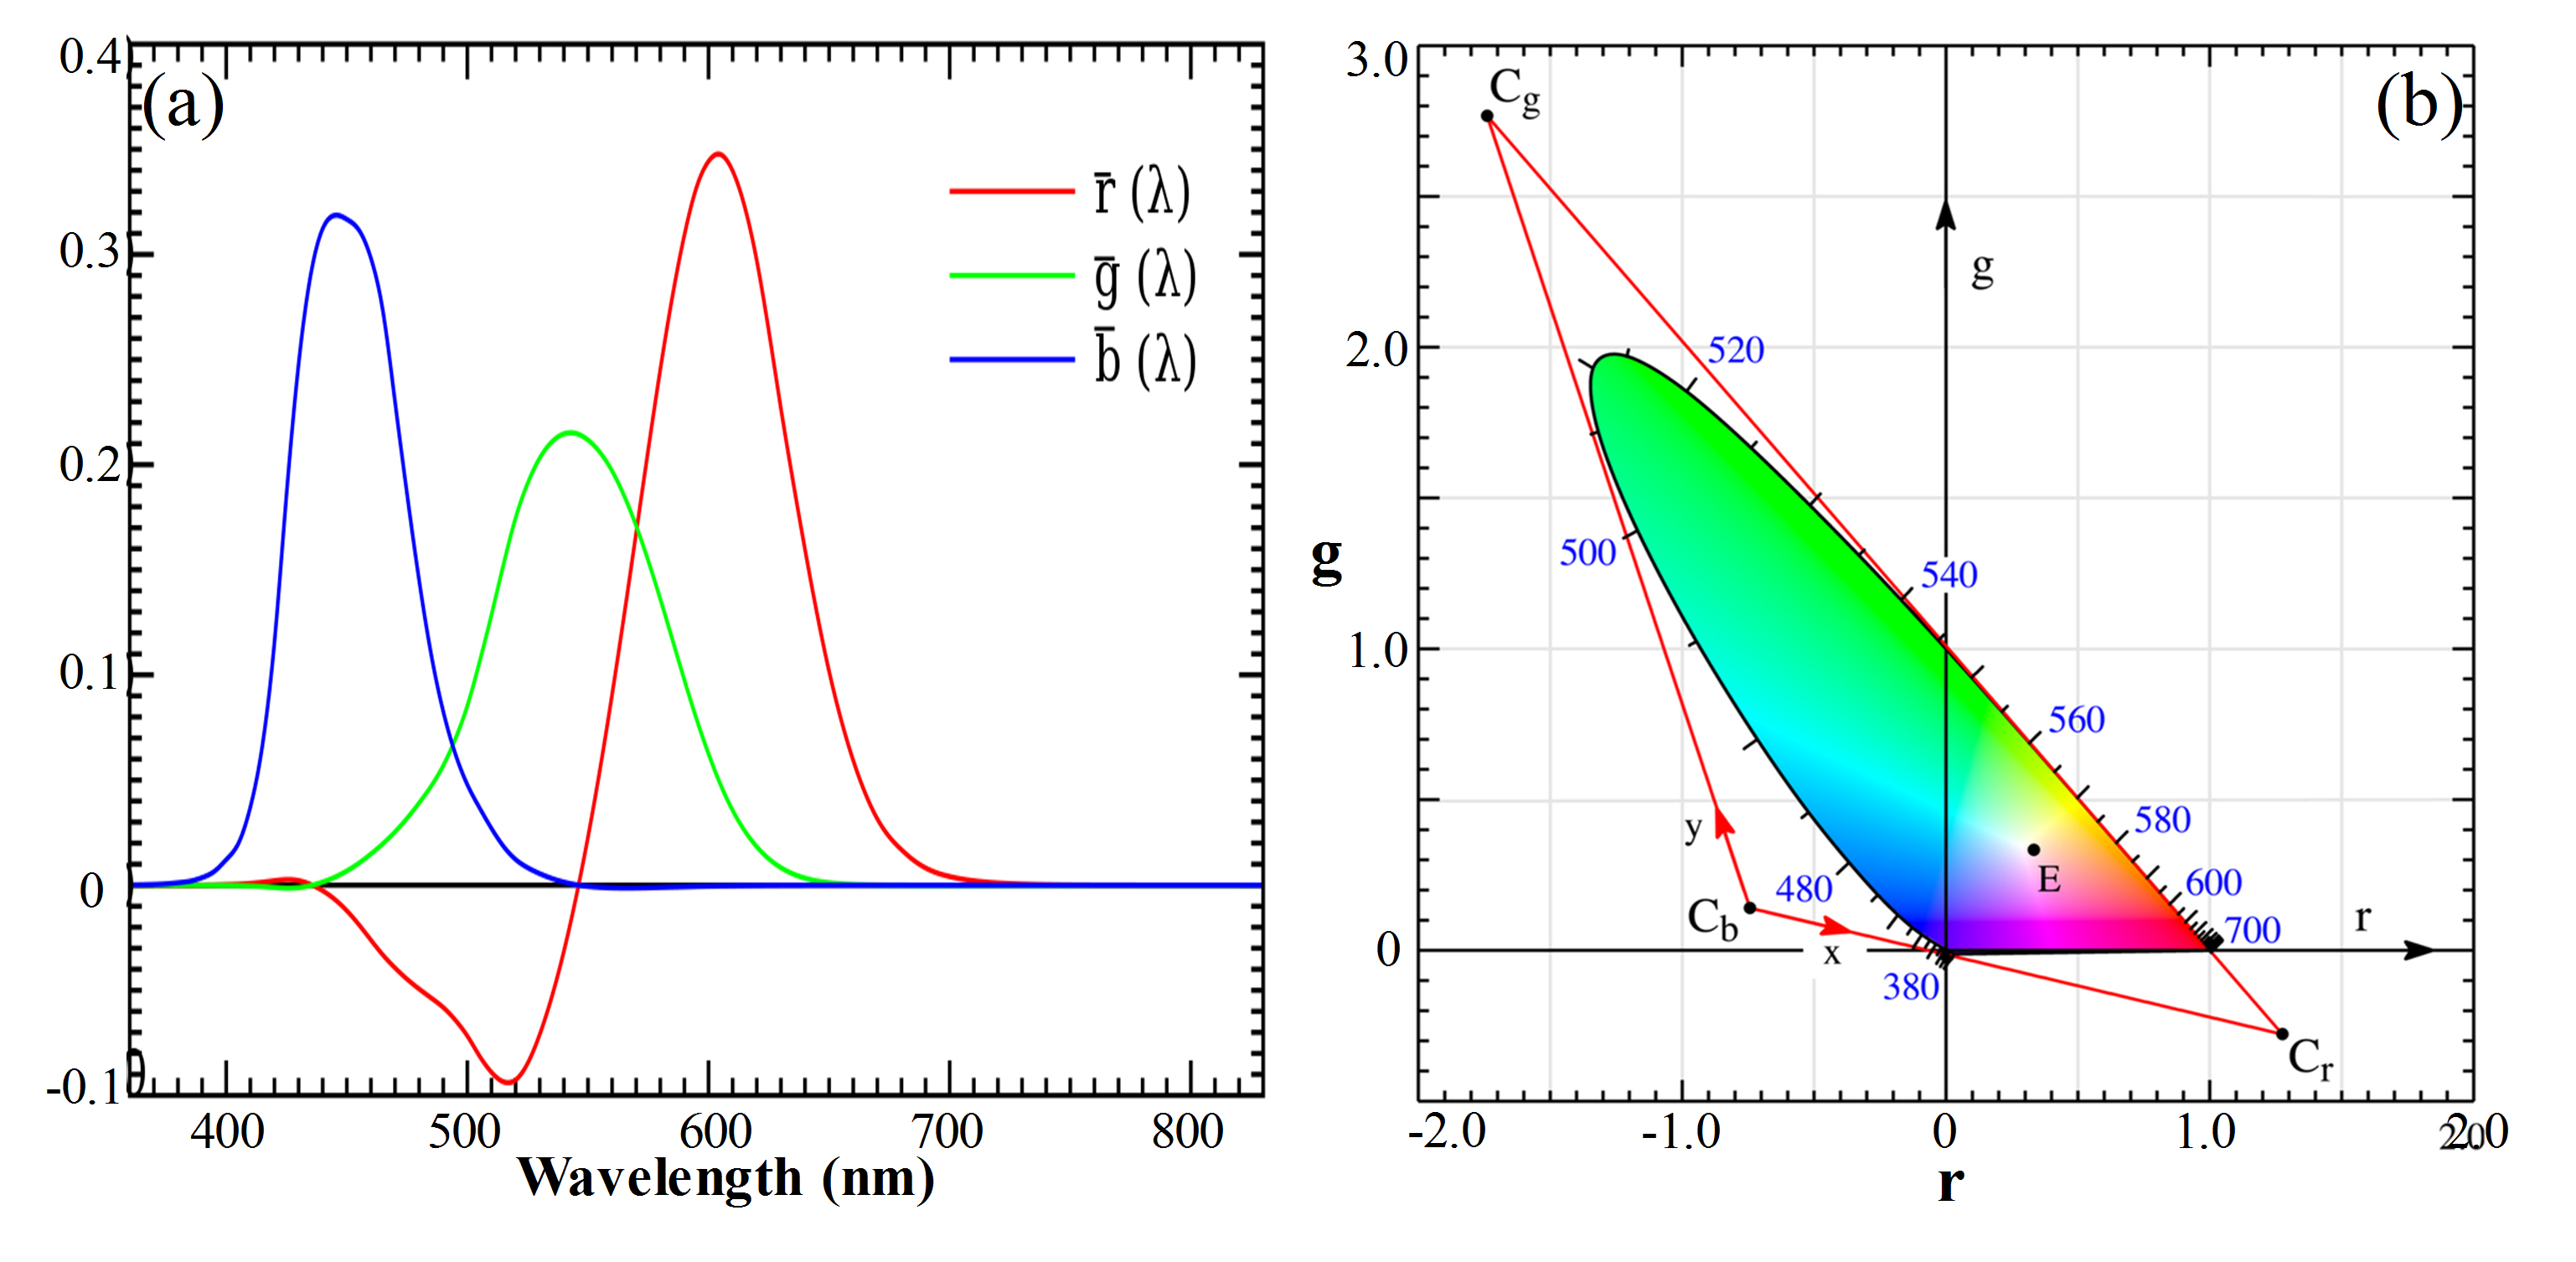
\includegraphics[width=16cm]{./Pictures/color_rgb_combined.jpg}
	\captionsetup{justification=centering}
	\caption{(a)~CIE1931~RGB色度系统光谱三刺激值曲线;(b)~CIE1931~RGB色品图\cite{wikicie1931}}
	\label{color_rgb_combined}
\end{figure}

在颜色研究和度量中,一般不用颜色的三刺激值R、G、B来表示颜色,而是用三刺激值各自在三刺激总量R+G+B中所占的比例来表示颜色,也叫做色品。选用R、G、B为三原色时,用r、g、b来表示色品坐标,有:
\begin{equation}
\label{sepin}
r=\dfrac{R}{R+G+B};~g=\dfrac{G}{R+G+B};~b=\dfrac{B}{R+G+B}
\end{equation}
且r~+~g~+~b~=~1。当计算光谱色的色品坐标时,只需要将R、G、B替换为$\overline{r}(\lambda)\mbox{、}\overline{g}(\lambda)\mbox{、}\overline{b}(\lambda)$即可,结果如图\ref{color_rgb_combined}(b)所示,图中马蹄形曲线为光谱色色品点轨迹,从图中给我们可以发现有的颜色的色品坐标是负的,这既不便于计算,也难于理解,因此CIE同时推荐了另一色度学系统,即CIE1931-XYZ系统。

\subsection{CIE1931-XYZ系统}
CIE1931-XYZ系统选用了X、Y、Z为三原色,该三原色的选取遵循规则如下:
\begin{enumerate}[(1)]
	\item 
	用此三原色匹配等能光谱色,三刺激值不应出现负值。
	\item 
	实际不存在的颜色在色品图上所占的面积应尽量小。
	\item 
	用Y刺激值表示颜色的亮度,同时亦表示色度;而X和Z刺激值只表示色度,不代表亮度。
\end{enumerate}

根据以上原则,求出X、Y、Z三原色在CIE1931-RGB中的色品坐标如表\ref{coordinate_XYZ}所示,此时X、Y、Z三原色并不实际存在,只是3个虚拟的颜色,故不能用来进行配色实验得到三刺激值曲线。CIE根据RGB的三刺激曲线经过坐标转换和定标,得到CIE1931XYZ系统下的三刺激值曲线,也叫CIE1931标准色度观察者光谱三刺激值曲线,如图\ref{color_xyz_combined}(a)所示。从中可以看出,刺激值已经没有负值。

\begin{table}[htb]
	\zihao{5}
	\captionsetup{justification=centering}
	\caption{XYZ三原色在RGB系统中的色品坐标}
	\label{coordinate_XYZ}
	\centering
	\begin{tabular}[t]{|cccc|}
		\hline
		& r & g & b  \\
		\hline
		(X) & 1.2750 & -0.2778 & 0.0028  \\
		\hline
		(Y)	& -1.7392 & 2.7671 & -0.0279  \\
		\hline
		(Z)	& -0.7431 & 0.1409 & 1.6022  \\
		\hline
	\end{tabular}
\end{table}

\begin{figure}[htb]
	\centering
	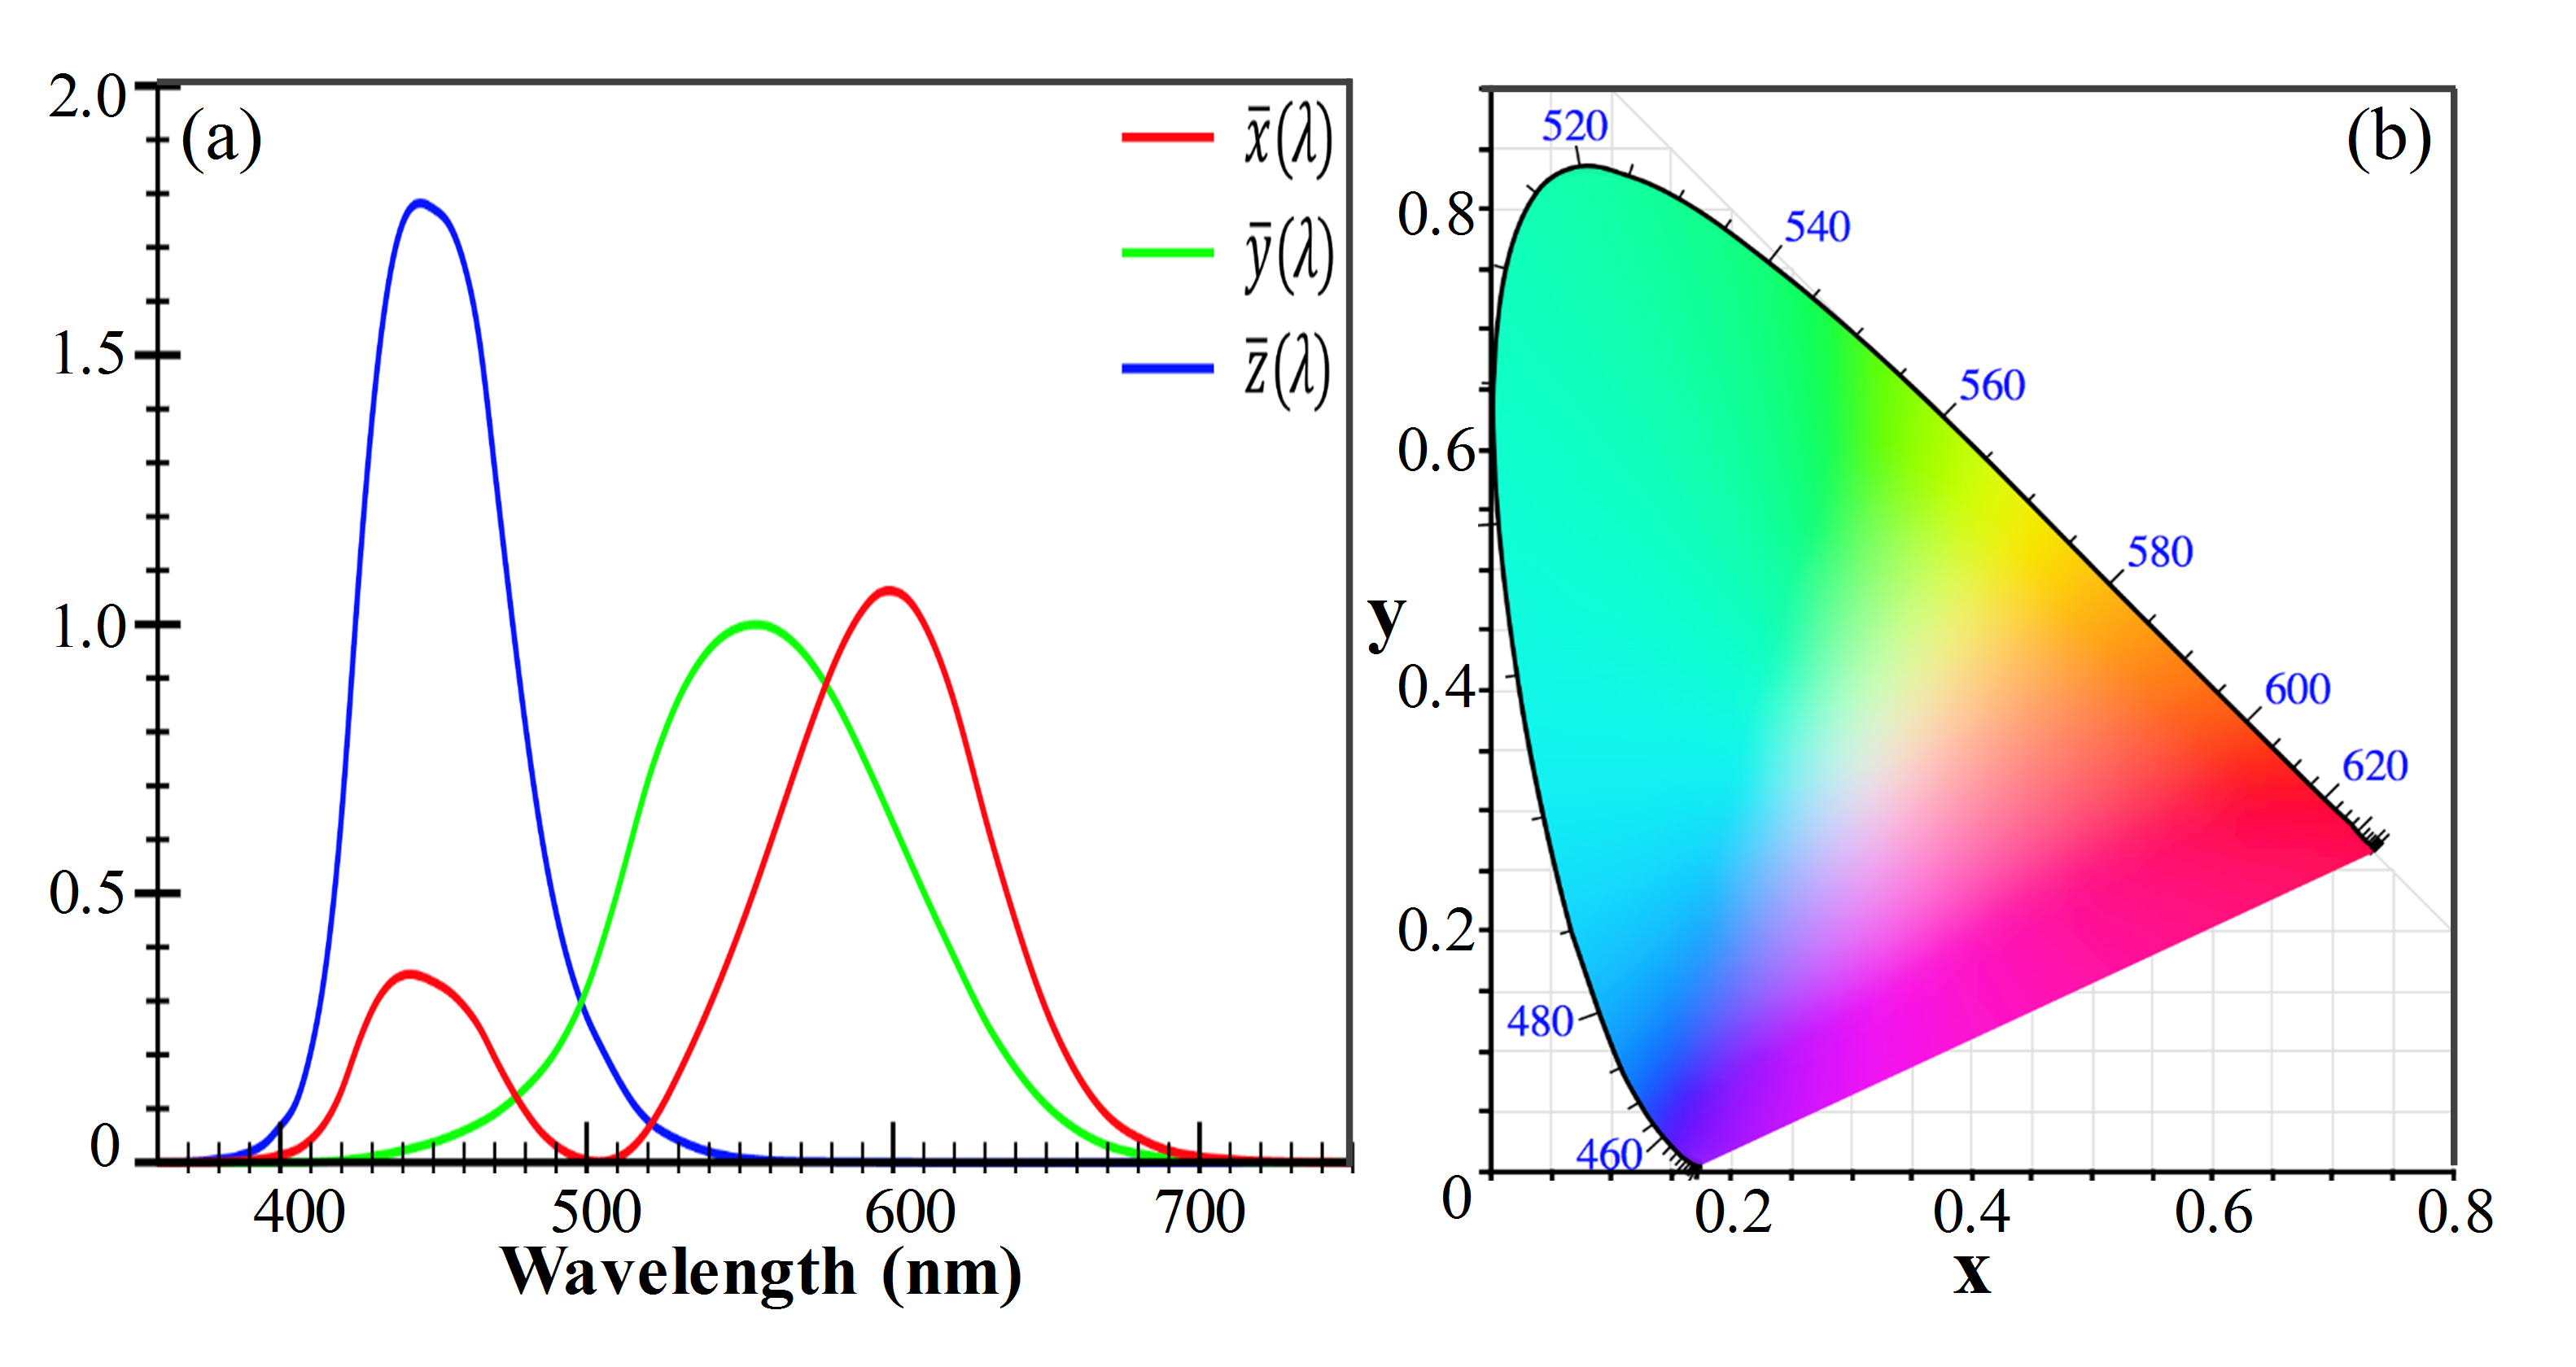
\includegraphics[width=16cm]{./Pictures/color_xyz_combined.jpg}
	\captionsetup{justification=centering}
	\caption{(a)~CIE1931~XYZ色度系统光谱三刺激值曲线;(b)~CIE1931~XYZ色品图\cite{wikicie1931}}
	\label{color_xyz_combined}
\end{figure}

与CIE1931-RGB系统类似,我们也可定义CIE1931-XYZ系统的色品坐标为:
\begin{equation}
\label{sepin_XYZ}
x=\dfrac{X}{X+Y+Z};~y=\dfrac{Y}{X+Y+Z};~z=\dfrac{Z}{X+Y+Z}
\end{equation}
且x~+~y~+~z~=~1。据此得到CIE1931色品图,如图\ref{color_xyz_combined}(b)所示。


至此,如果我们已知颜色刺激的波长分布$\varphi(\lambda)$,即不同波长上的辐射能通量,我们就可以根据公式\ref{stimulate_X}\~{}\ref{stimulate_Z}求得颜色的三刺激值,以及色品坐标。

\begin{equation}
\label{stimulate_X}
X=k\int_{380}^{780}\varphi(\lambda)\overline{x}(\lambda)d\lambda
\end{equation}
\begin{equation}
\label{stimulate_Y}
Y=k\int_{380}^{780}\varphi(\lambda)\overline{y}(\lambda)d\lambda
\end{equation}
\begin{equation}
\label{stimulate_Z}
Z=k\int_{380}^{780}\varphi(\lambda)\overline{z}(\lambda)d\lambda
\end{equation}
其中$k=\dfrac{100}{Y}$,因为CIE规定Y刺激值为1或者100,为显示设备支持的最亮的白色。由于$\overline{x}(\lambda)$、$\overline{y}(\lambda)$、$\overline{z}(\lambda)$等参数常常以一定波长间隔的离散形式给出,所以在实际计算时,常常用求和的方式代替积分。

\subsection{CIE-XYZ坐标转换为CIE-RGB坐标}
由XYZ色坐标系统的定义可知,其为RGB系统的线性变换。我们采用sRGB来表示最后计算得到的颜色,sRGB为RGB的一种,其三原色的xyz坐标点如表\ref{sRGBxyz}所示。然后可以用公式\ref{XYZ2RGB}\cite{international1999iec}将XYZ刺激值转换为RGB三刺激值,再得出rgb色品坐标。
\begin{table}[htb]
	\zihao{5}
	\captionsetup{justification=centering}
	\caption{sRGB三原色与参考白xyY坐标点}
	\label{sRGBxyz}
	\centering
	\begin{tabular}[t]{|ccccc|}
		\hline
		& Red & Green & Blue & White point \\
		\hline
		x & 0.6400 & 0.3000 & 0.1500 & 0.3127 \\
		\hline
		y	& 0.3300 & 0.6000 & 0.0600 & 0.3290 \\
		\hline
		Y	& 0.2126 & 0.7152 & 0.0722 & 1.0000 \\
		\hline
	\end{tabular}
\end{table}

\begin{equation}
\label{XYZ2RGB}
\left[\begin{array}{c}
R\\
G\\
B
\end{array}
\right]=
\begin{bmatrix}
3.2406 & -1.5372 & -0.4986\\
-0.9689 & 1.8758 & 0.0415\\
0.0557 & -0.2040 & 1.570
\end{bmatrix}
\begin{bmatrix}
X\\Y\\Z
\end{bmatrix}
\end{equation}

由于显示器的亮度显示是非线性的,我们还需用公式\ref{gamma}对所得的rgb值进行伽马校正\cite{international1999iec}。

\begin{equation}
\label{gamma}
c_{srgb} = \left\{
\begin{array}{lcc}
12.92c_{rgb}, &     & c_{rgb}\le0.0031308\\
(1+a)c_{rgb}^{1/2.4}-a,&     & c_{rgb}>0.0031308
\end{array}
	\right.
\end{equation}
其中a~=~0.055,c表示r、g或者b坐标。

至此,我们就可以根据光谱先计算得到XYZ三刺激值,利用转换矩阵得到RGB三刺激值,然后得到rgb色品坐标,经过伽马校正之后,我们就可以得到最终颜色的rgb值。

\section{SOI色谱图的计算}
我们采用Lumerical FDTD Solutions\cite{fdtdsolution}来仿真硅薄层的反射率,仿真模型如图\ref{color_reflection}(a)所示。图\ref{color_reflection}(b)显示了150~$nm$硅层厚度下,不同波长的光的反射率,从中可以明显看出薄膜干涉现象,而且因为硅在可见光波段具有明显的吸收,该反射谱还包含了吸收的信息。具体建模过程描述如下:

\begin{figure}[htb]
	\centering
	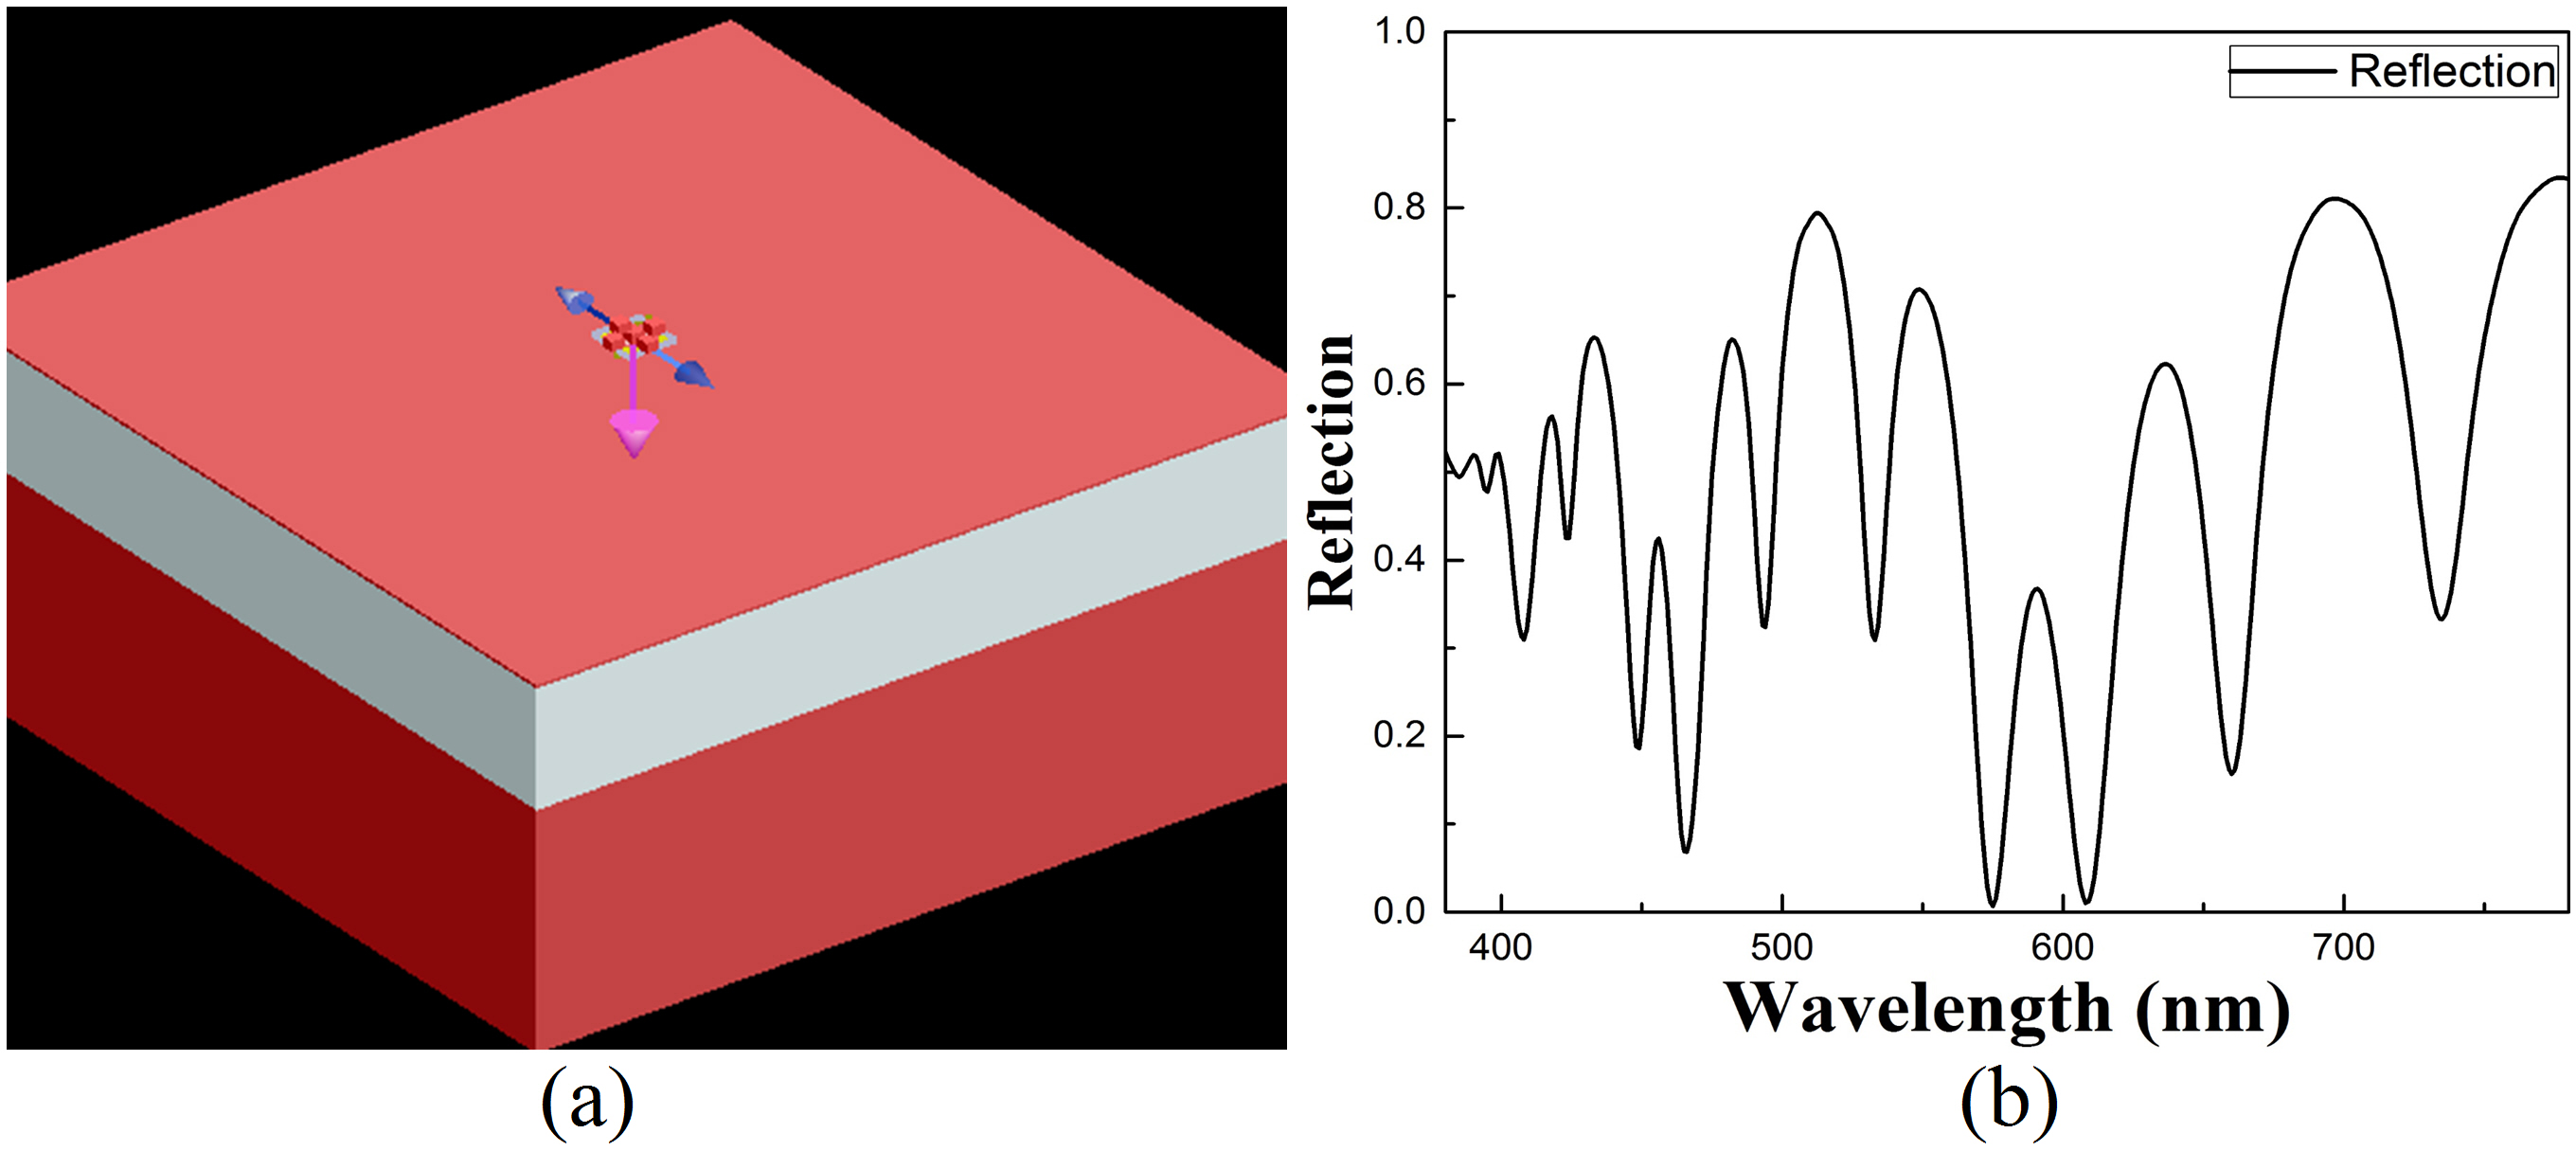
\includegraphics[width=14cm]{./Pictures/color_reflection.jpg}
	\captionsetup{justification=centering}
	\caption{SOI硅薄层(a)仿真模型;(b)仿真得到150~$nm$硅层厚度的反射率}
	\label{color_reflection}
\end{figure}

\begin{enumerate}[(1)]
	\item 
	仿真结构的建立与材料的选取:仿真的结构是基于实际SOI平芯片设置,衬底设为硅,二氧化硅氧化层的厚度为2~$\mu m$,硅层厚度扫描从0~\~{}~220~$nm$,上包层为空气。材料折射率采用软件内部使用的Palik测定值。
	\item 
	FDTD仿真区域与边界条件的设置:结构确定之后需要设置仿真区域,采用3D FDTD进行仿真,当硅层厚度比较薄时,光可以穿透硅层到达衬底,故我们将仿真区域延伸到衬底当中。边界条件的设置:在水平方向上设置为周期边界条件,来模拟无穷大的硅层。上下边界条件设为完美匹配层(Perfectly matched layer, PML)来模拟无穷大的空间。
	\item 
	仿真光源的选取:假设我们在日光下观察SOI芯片,故仿真中我们用平面光源来模拟实际情况。仿真的波长范围设置为380~\~{}~780~$nm$。
	\item 
	求解区域的网格划分:根据第二章中对时域有限差分方法的描述,在仿真计算过程中需要对求解区域进行网格划分,我们采用软件提供的自适应网格技术对网格进行划分,划分精度为3,如图\ref{color_mesh}所示。可以看到在硅层,因为折射率较高,所以网格划分也较为致密。
	\begin{figure}[htb]
		\centering
		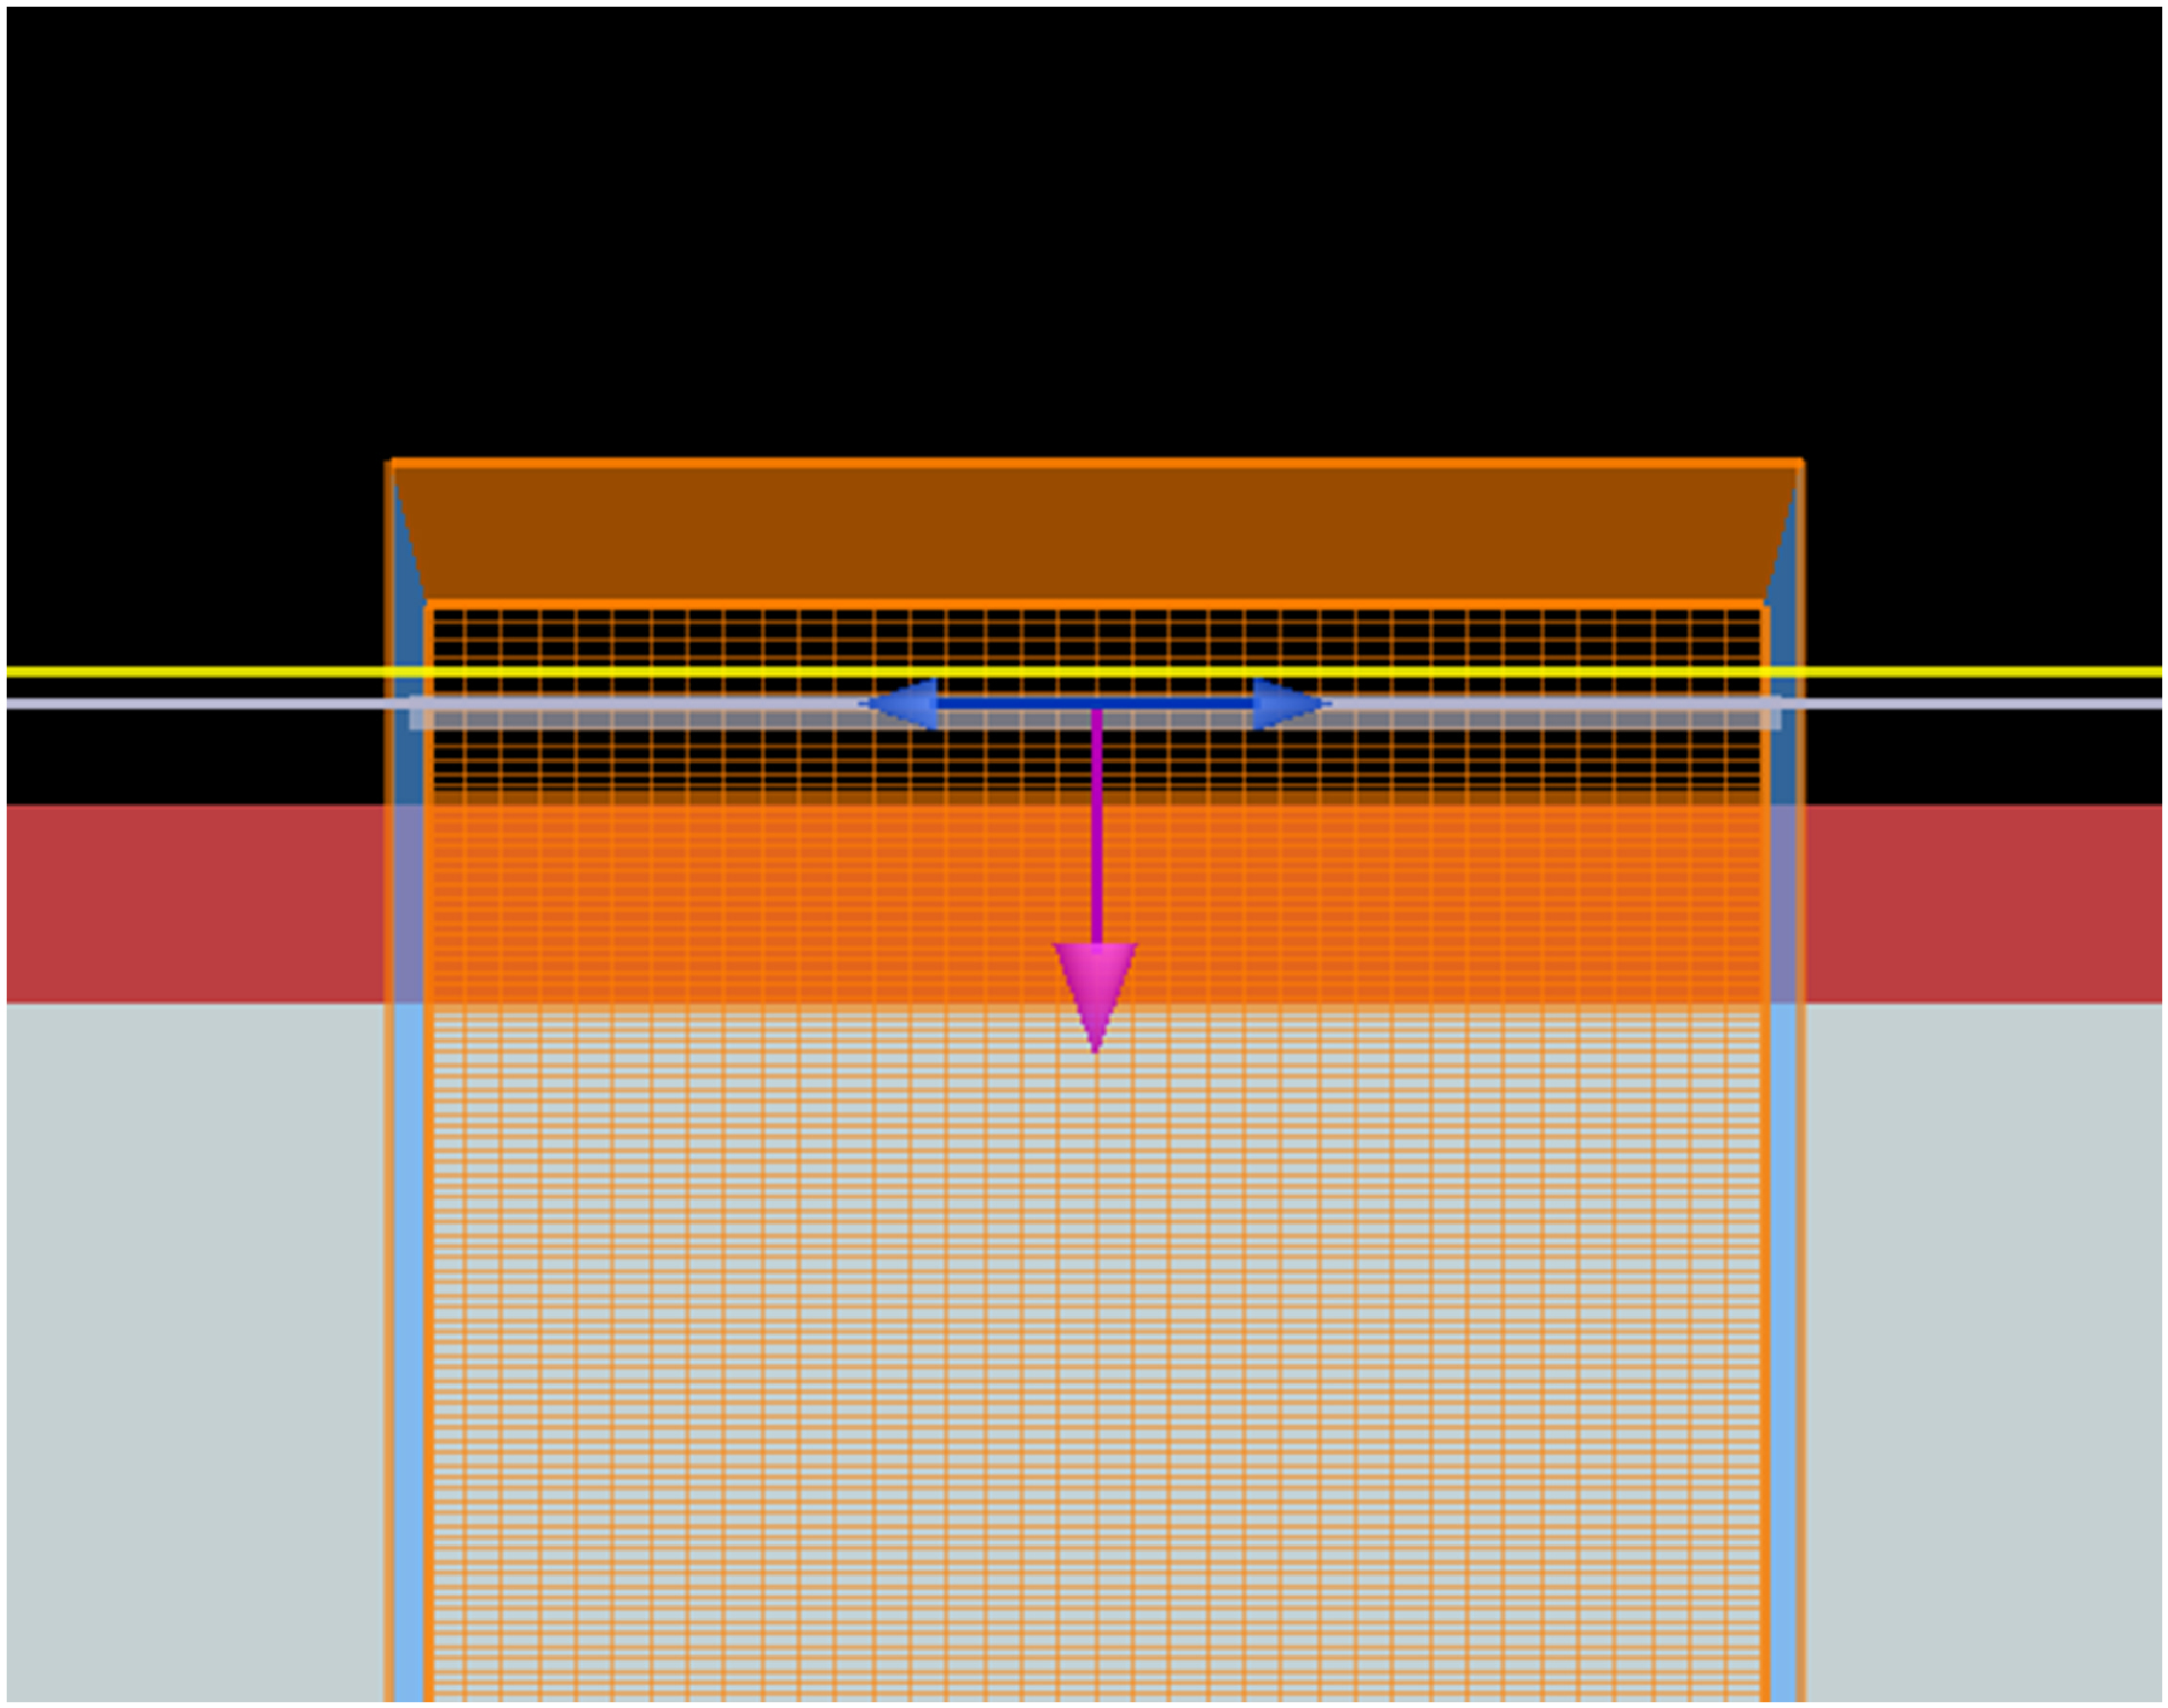
\includegraphics[width=10cm]{./Pictures/color_mesh.jpg}
		\captionsetup{justification=centering}
		\caption{FDTD solutions仿真区域网格划分}
		\label{color_mesh}
	\end{figure}
	\item 
	功率监视器的设置:将功率监视器放置于光源上方来观察结构在不同波长入射光下的反射特性。
\end{enumerate}

用上述模型扫描SOI不同硅层厚度时的反射谱,我们得到图\ref{color_reflection_all}所示的结果.图中横坐标表示不同的波长,纵坐标为硅层的厚度,所以每一条横线表示某个硅层厚度下的反射谱。我们可以看到当硅层厚度较小时,短波长处的谐振峰强度较大,随着硅层厚度的增大,其强度慢慢减弱,可以预测当硅层厚度较小时,蓝色会比较明显。我们还可以看到当硅层厚度变化时,谐振峰的漂移较为连续,故应可以得到较为连续的颜色变化。

\begin{figure}[htb]
	\centering
	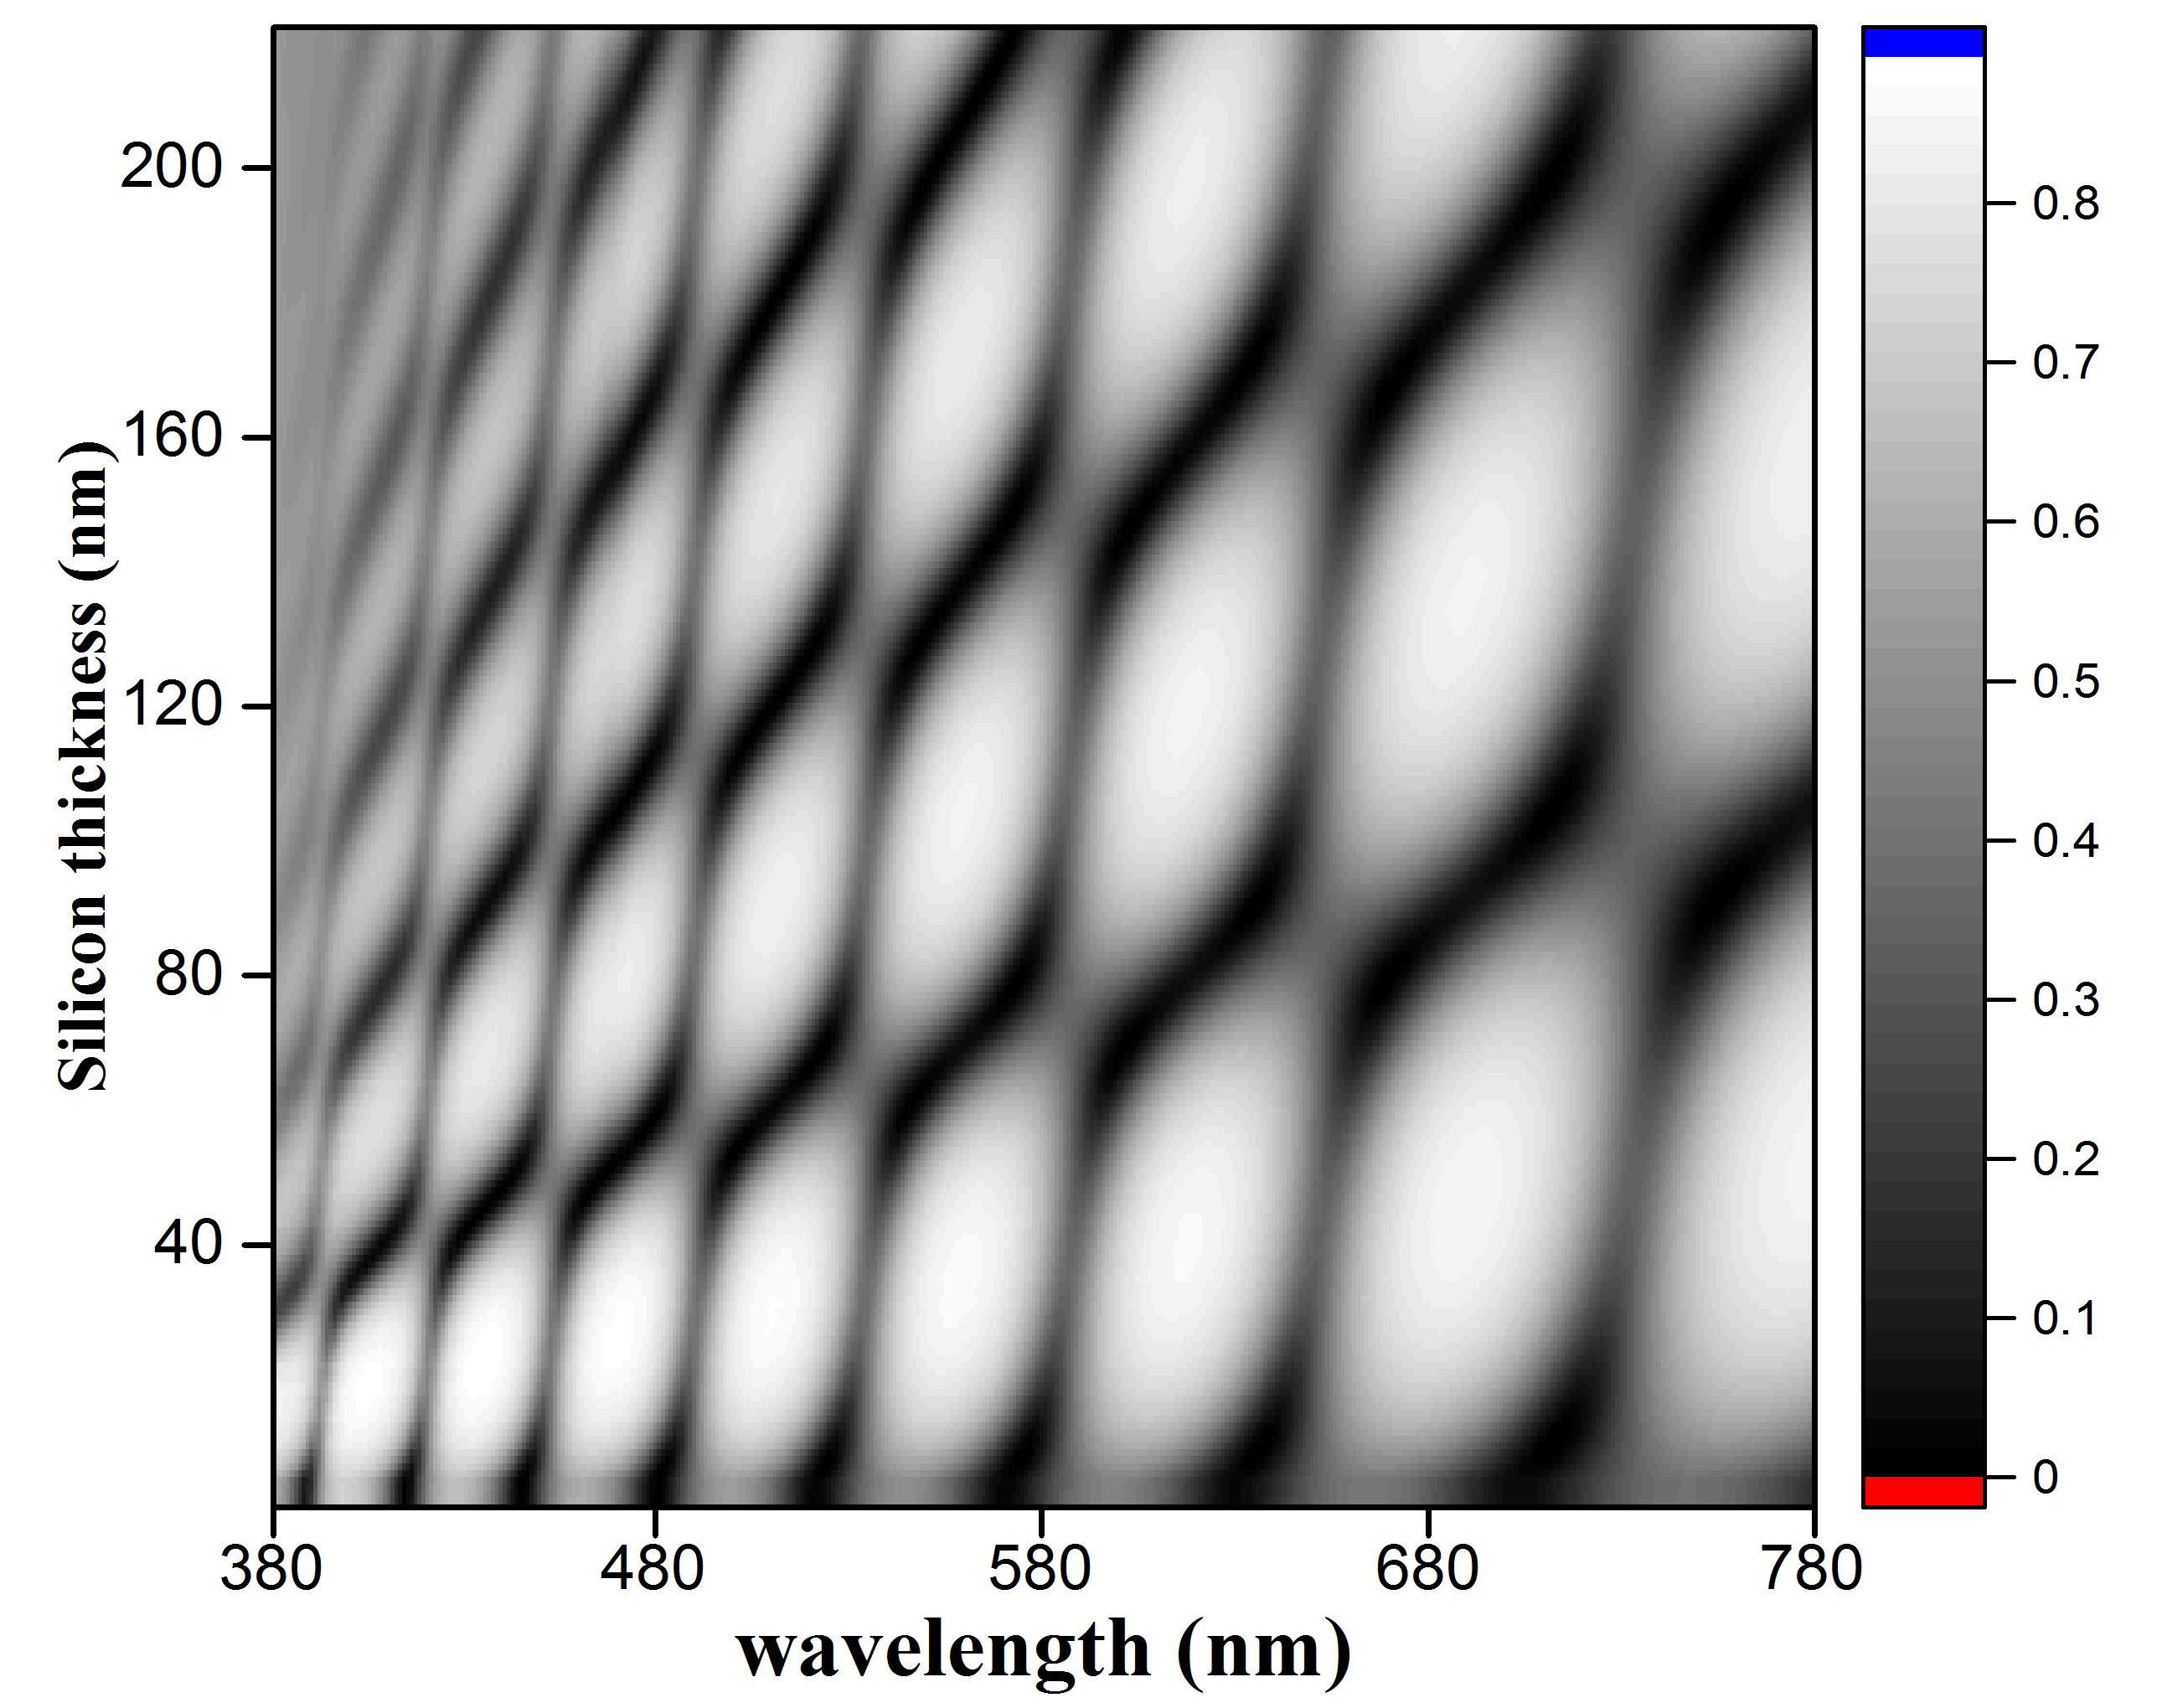
\includegraphics[width=12cm]{./Pictures/color_reflection_all.jpg}
	\captionsetup{justification=centering}
	\caption{FDTD solutions仿真得到不同硅层厚度下的反射谱}
	\label{color_reflection_all}
\end{figure}

得到了SOI芯片不同硅层厚度下的反射谱之后我们需要确定光源的光谱,因为对于SOI芯片来说它是不发光物体,根据上文所述,观察该类物体的光谱需要由光源和反射谱共同决定。假设在自然光下进行观察,采用日光光谱作为光源光谱,如图\ref{color_sun_spectrum}所示,我们只截取了太阳光谱中380~\~{}~780~$nm$这一段中的光谱,因为只有这一段与颜色有关,图中的光谱强度已经做了归一化处理。

\begin{figure}[htb]
	\centering
	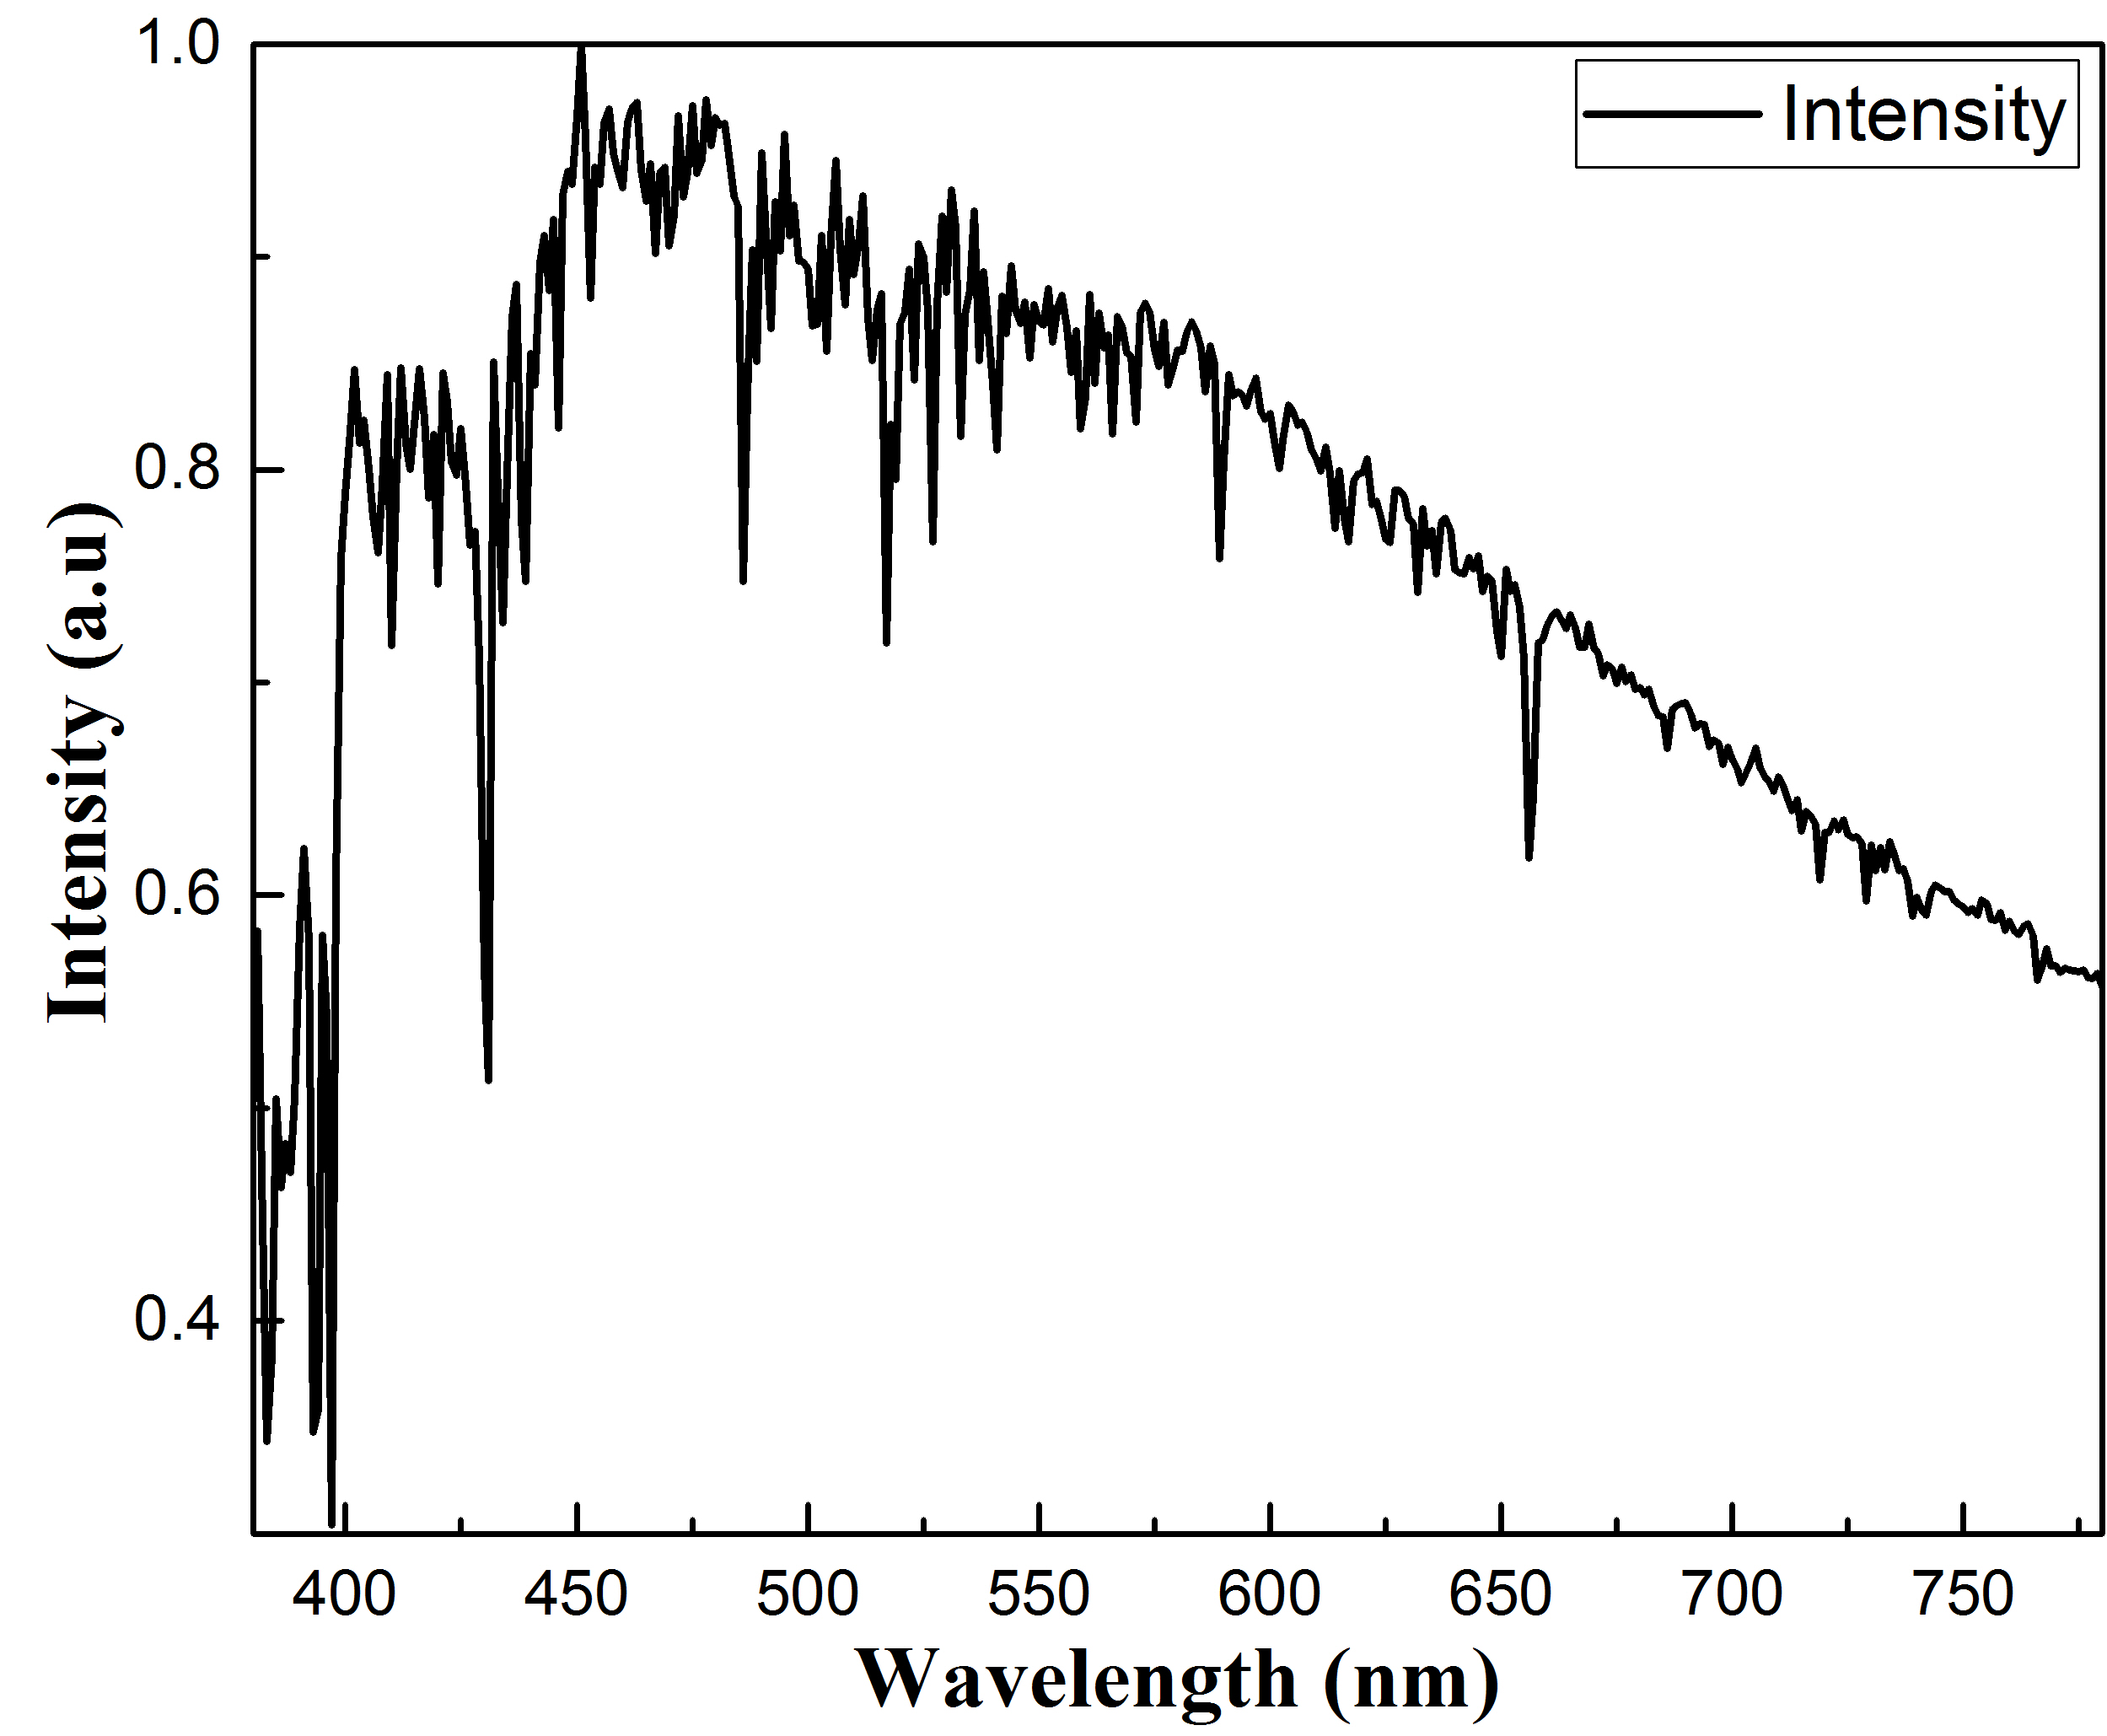
\includegraphics[width=12cm]{./Pictures/color_sun_spectrum.jpg}
	\captionsetup{justification=centering}
	\caption{380~nm~\~{}~780~nm波段的太阳光谱\cite{sunspectrum}}
	\label{color_sun_spectrum}
\end{figure}

将日光光谱与SOI芯片的反射谱相乘,得到最终用来计算色坐标的光谱之后,然后按上一节所述方法,计算得到不同硅层厚度对应的光谱的rgb坐标,显示之后的效果如图\ref{color_220nm}(a)所示,图中横坐标没有意义,只是重复了同一硅层厚度下的颜色以方便观察,纵坐标表示SOI芯片的硅层厚度。当硅层厚度为220~$nm$时,颜色显示为浅绿色,这与本章开头图\ref{color_wafer}(a)展示的硅层厚度为220~$nm$的标准SOI芯片的颜色是符合的。随着硅层厚度的减小,SOI芯片的颜色会先变成粉红,然后又变绿,再变粉红,之后会出现黄色,在硅层厚度在40~\~{}100~$nm$范围内时,颜色变化的信息非常丰富。这是由于硅的折射率实部很大,在可见光波段达到4以上,在波长为400~$nm$左右时,折射率甚至可以达到6左右,如图\ref{color_220nm}(b)所示,所以当硅层厚度减小时光程差变化比较大,干涉增强的波长值移动也会比较迅速。硅薄膜的颜色随厚度变化特性还跟硅对可见光的吸收相关,从图\ref{color_220nm}(c)中可以看到,硅对短波长的可见光比长波长的可见光吸收大,所以当硅薄膜厚度在100~$nm$以上时,短波长的可见光吸收较多,故颜色只有红、绿、黄色,缺少蓝色,当硅薄膜厚度减小到80~$nm$附近时,才有蓝色部分出现。当计算二氧化硅薄膜厚度变化的时候,颜色变化就会比硅缓慢很多且厚度较厚时也可以观察到蓝色。当硅层厚度小于40~$nm$之后,SOI芯片就只会显示出灰度的变化,并且随着硅层厚度降低,灰度值也越来越高。这个因硅层厚度减小而颜色发生变化的情形与肥皂泡的破裂很类似,我们知道,当肥皂泡刚形成时,形成肥皂泡的水膜比较厚,当可见光照射时,总会有某些波长得到干涉增强,某些波长干涉相消,从而产生彩色,而且随着水膜因为蒸发厚度较小时,干涉增强的波长会不停地发生变化,故我们可以看到肥皂泡的颜色不停地发生变化。当水膜减薄到一定程度后,就无法形成可见光波段的干涉增强,此时就没有彩色,故当肥皂泡的彩色消失时,说明肥皂泡的厚度也减小到了一定程度,离破裂也就不远了。在这里,SOI芯片的硅层就像肥皂泡的水膜,当彩色快消失时,说明硅层厚度也所剩无几了。

\begin{figure}[htb]
	\centering
	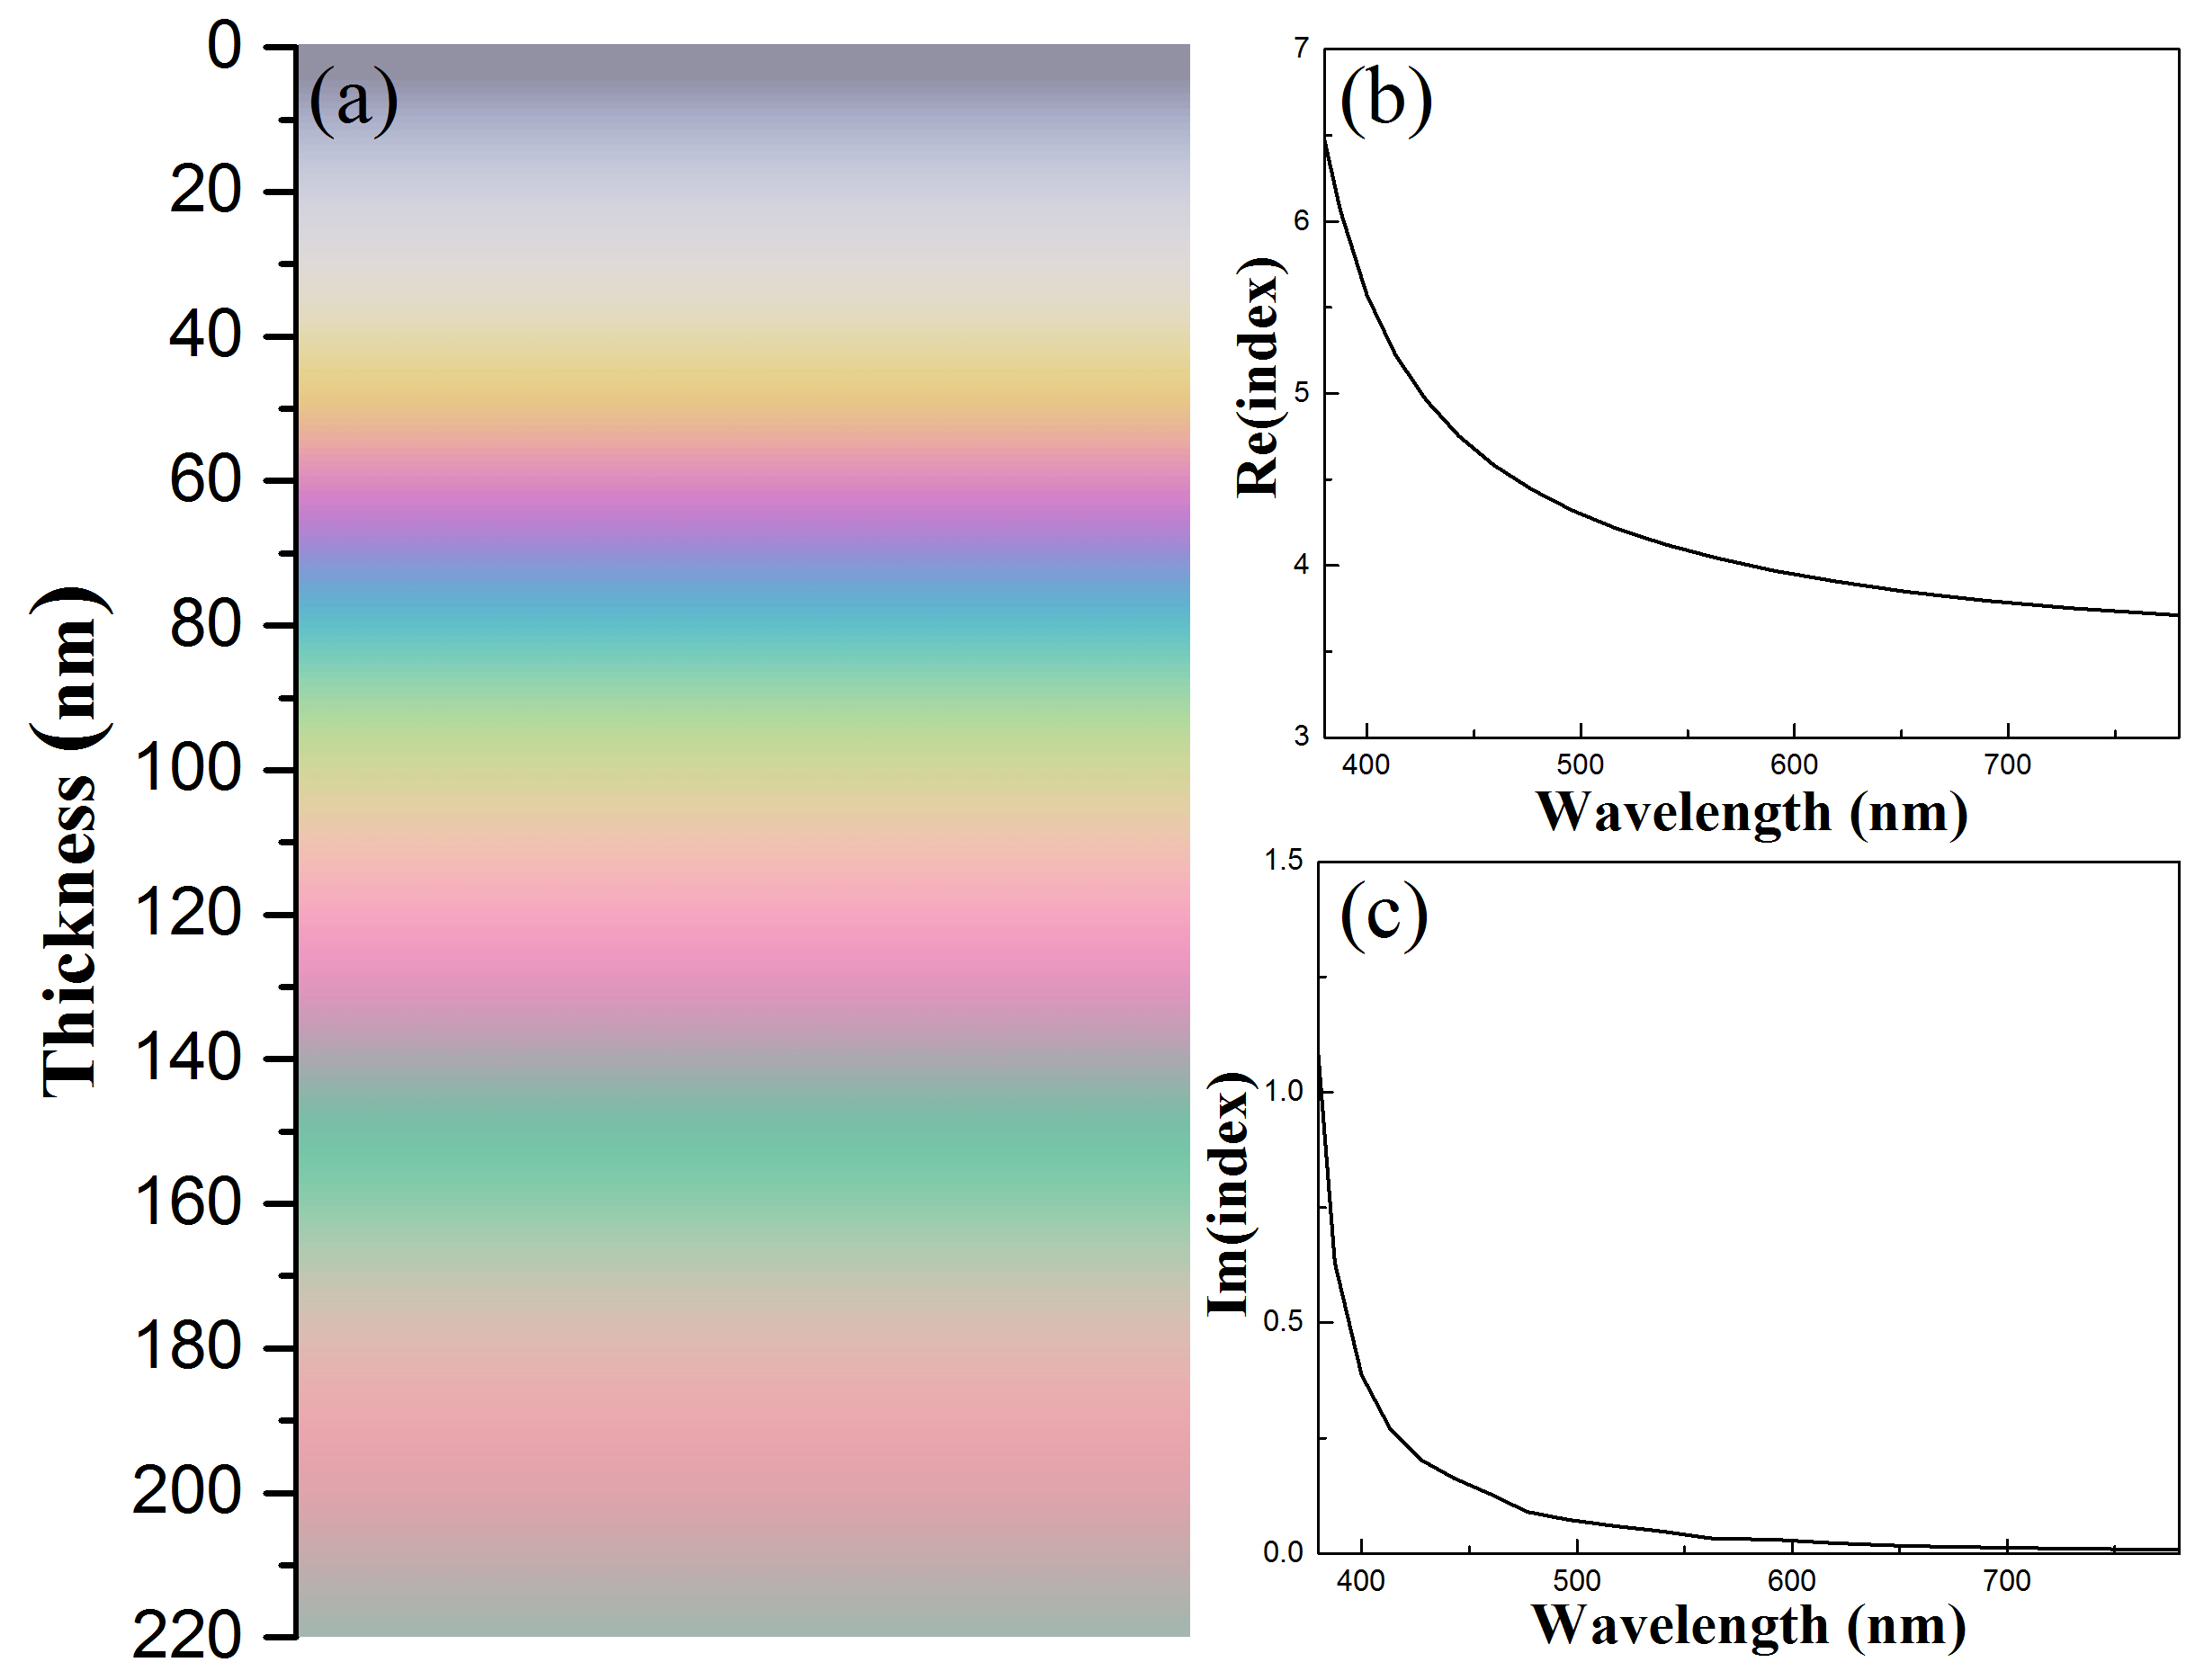
\includegraphics[width=14cm]{./Pictures/color_220nm.jpg}
	\captionsetup{justification=centering}
	\caption{(a)~0~\~{}~220~$nm$硅层厚度SOI芯片的色谱图;(b)硅在可见光波段的折射率实部;(c)硅在可见光波段的折射率虚部\cite{aspnes1983dielectric}}
	\label{color_220nm}
\end{figure}

为了比较不同角度入射光时观察到的颜色变化,我们计算了光源在30$^{\circ}$和60$^{\circ}$入射情况下SOI芯片随厚度变化的色谱图,如图\ref{color_compare}所示。我们可以看到当入射角度不同时,颜色变化很小,只是角度增大时,颜色明度值有所下降,这是由于入射角度增大时,反射率有所降低。根据计算结果,我们可以知道,当SOI芯片的硅层厚度确定之后,其颜色随观察角度的变化不明显,这个特性为我们接下来利用肉眼进行颜色比较确定硅层厚度提供了理论上的保证,因为SOI芯片表面光滑,往往会形成镜面反射从而使人脸成为背景色,影响颜色的判断。

\begin{figure}[htb]
	\centering
	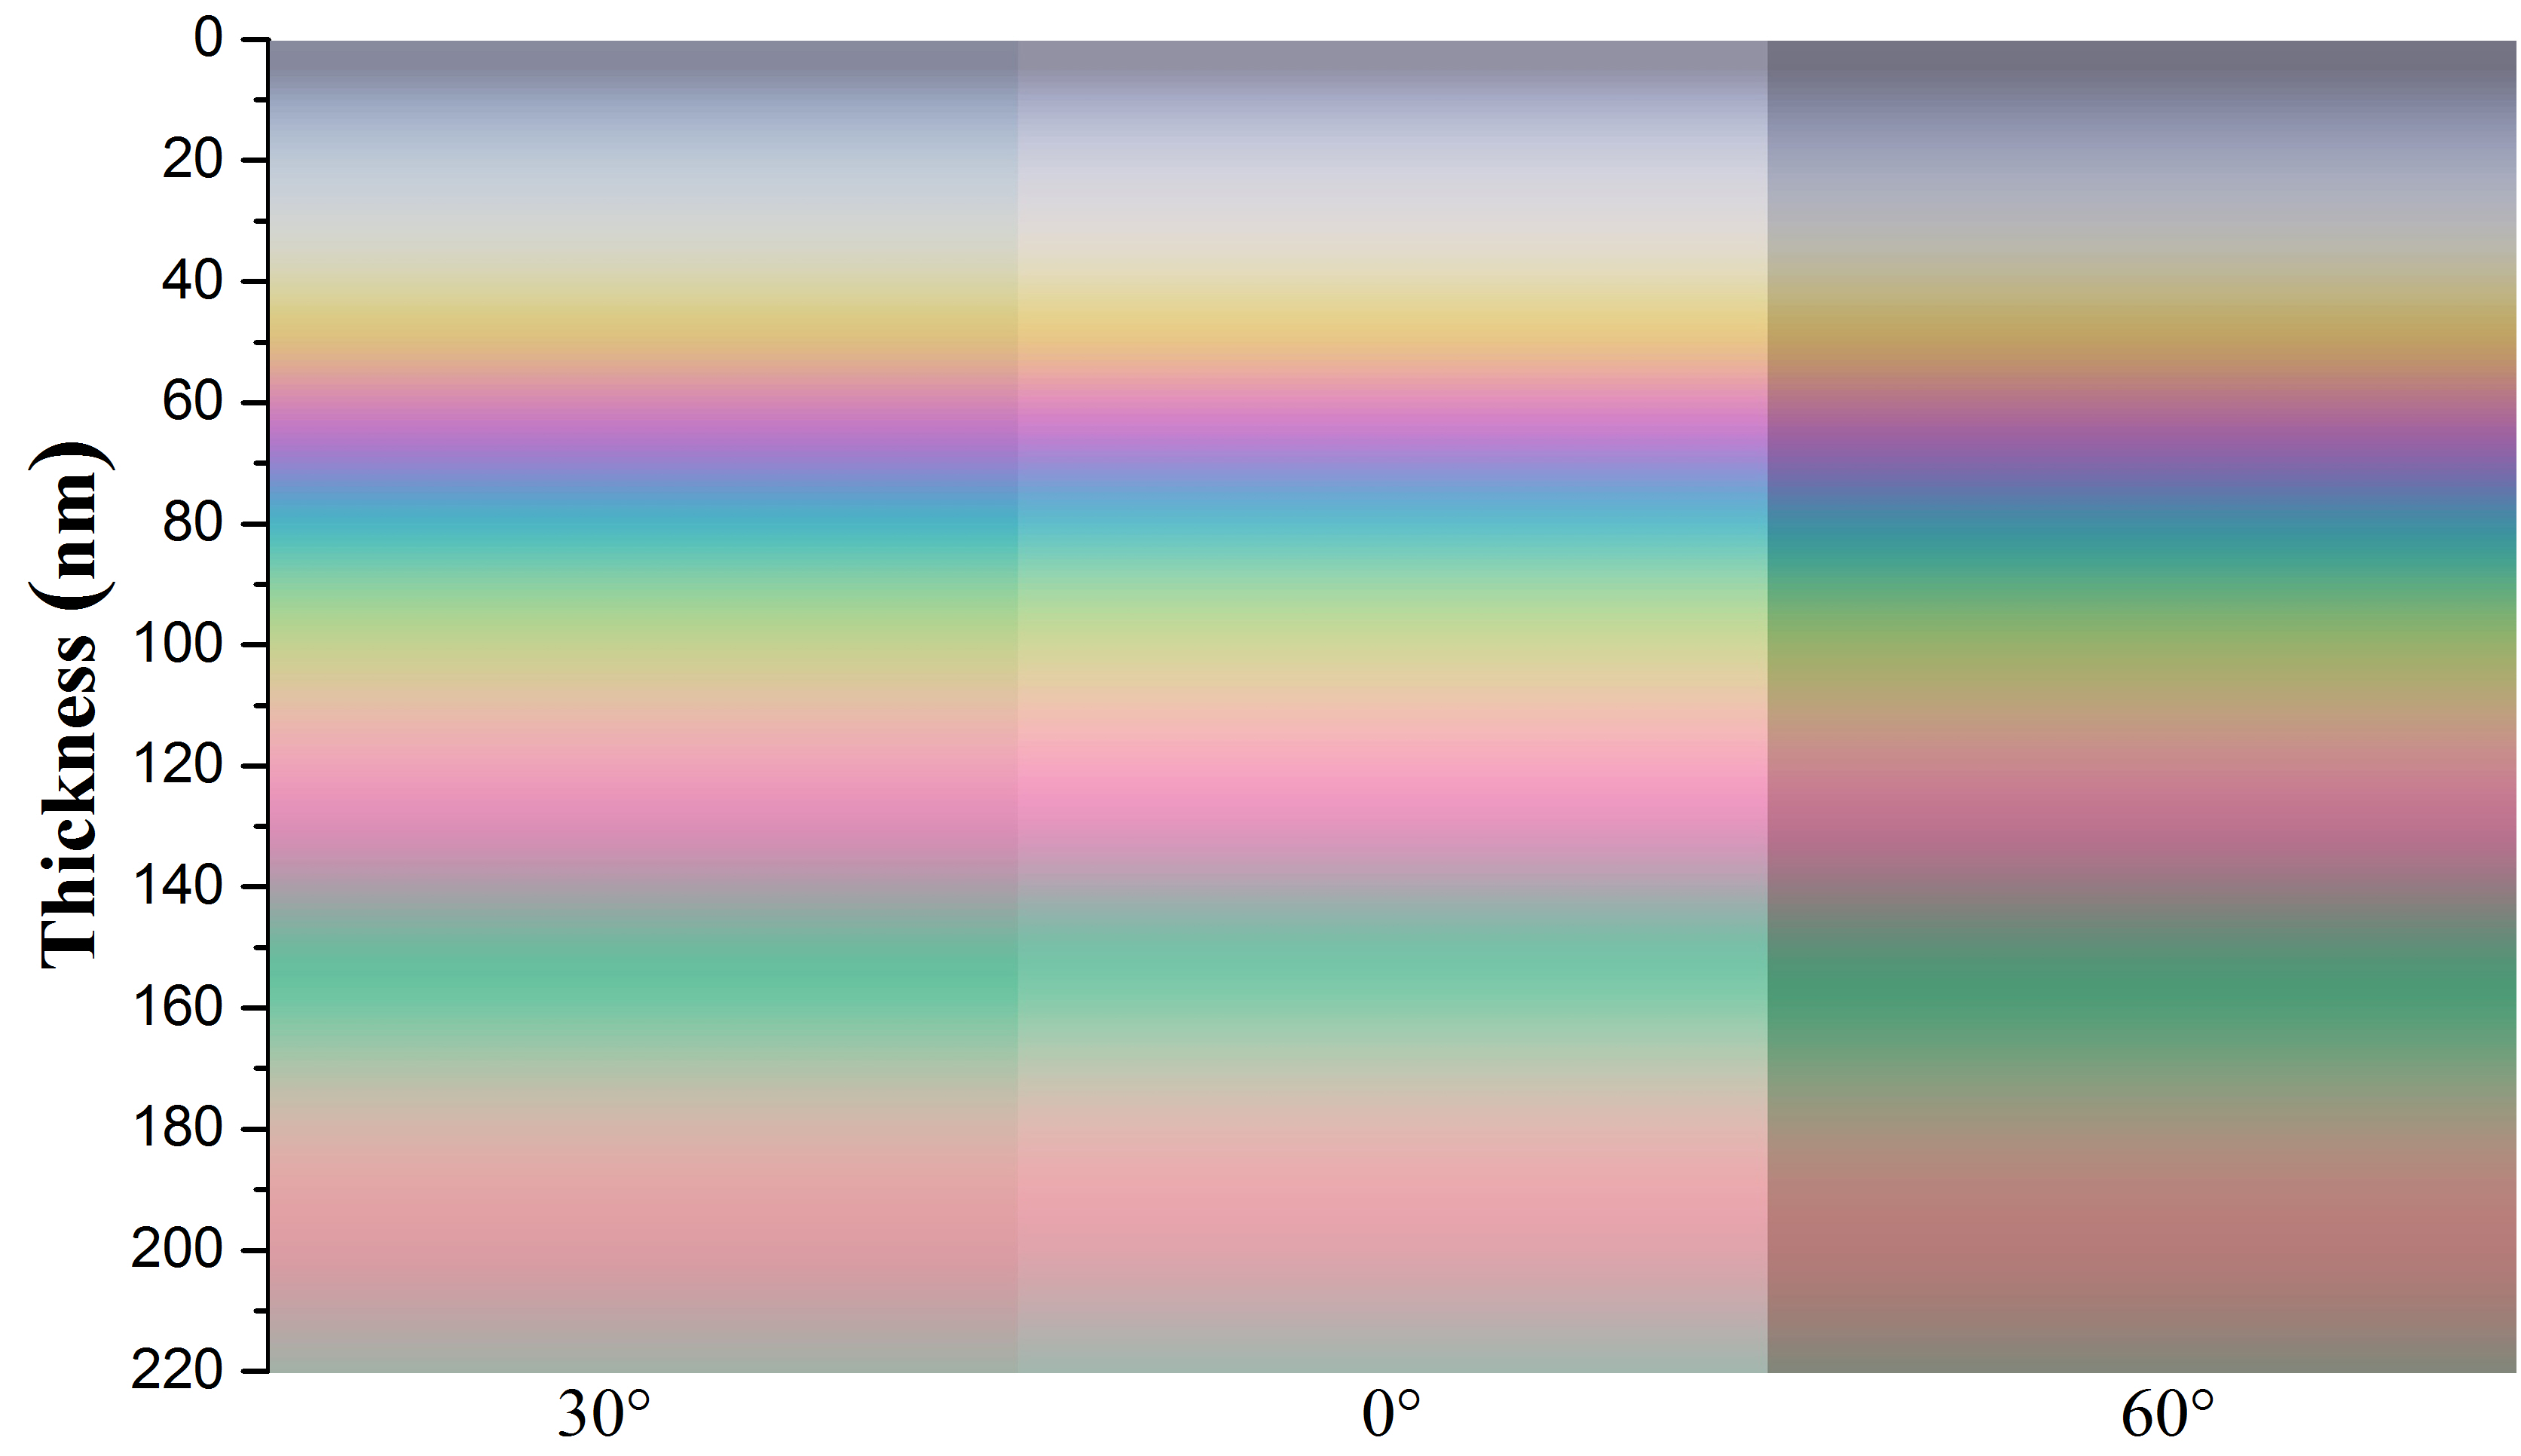
\includegraphics[width=14cm]{./Pictures/color_compare.jpg}
	\captionsetup{justification=centering}
	\caption{0$^{\circ}$、30$^{\circ}$、60$^{\circ}$观察时的色谱图}
	\label{color_compare}
\end{figure}

\section{颜色比较法测定硅层厚度}

为了方便颜色的比较,我们专门开发了一款叫做SOIEtch的手机APP,可以将色谱图中的颜色放大连续呈现,方便与芯片进行比较与匹配,软件截图如图\ref{color_app}所示。当上下滑动屏幕选取不同硅层厚度时,对应厚度的颜色会被放大呈现,选取与刻蚀之后的芯片颜色最相近的颜色,即可确定SOI芯片的硅层厚度。

\begin{figure}[htb]
	\centering
	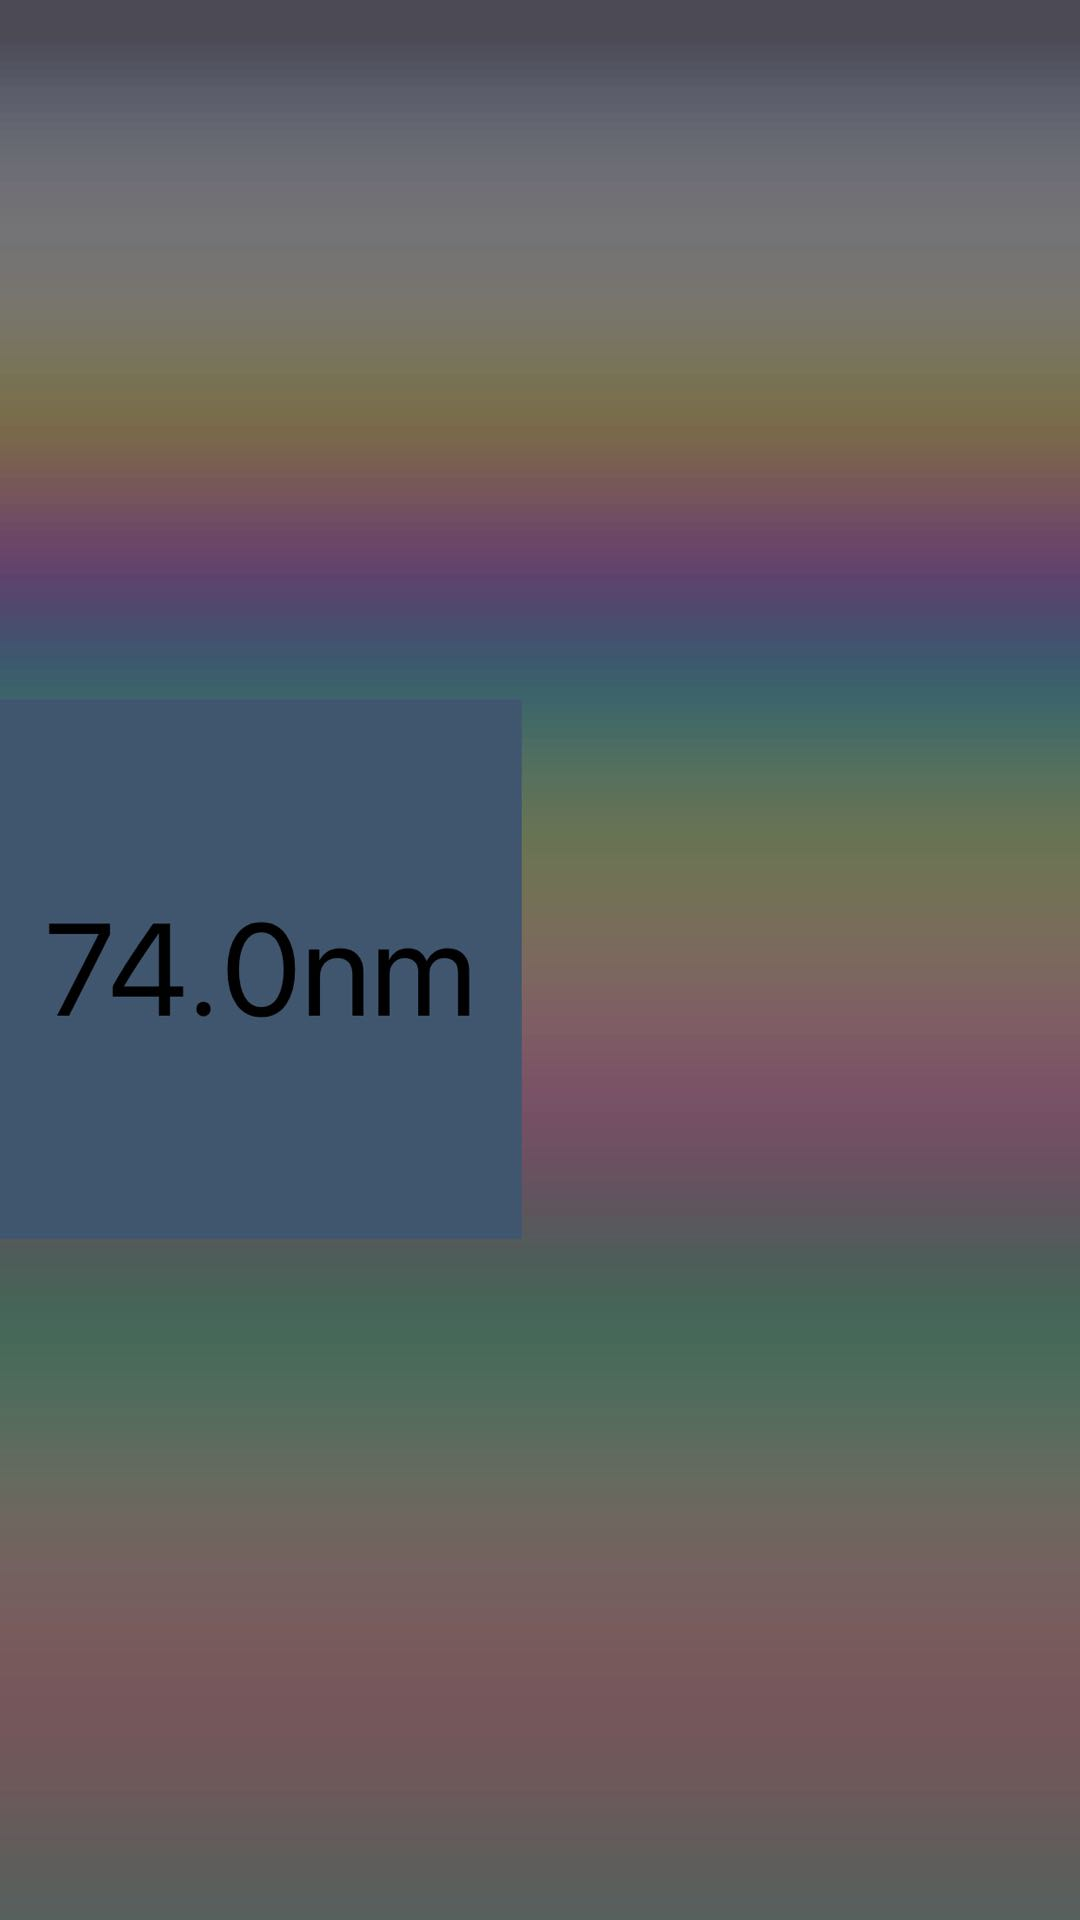
\includegraphics[width=6cm]{./Pictures/color_app.jpeg}
	\captionsetup{justification=centering}
	\caption{SOIEtch软件截图,插图为硅层厚度为74~$nm$时SOI芯片呈现的颜色}
	\label{color_app}
\end{figure}

我们制作了多组不同硅层厚度的SOI芯片,部分SOI芯片如图\ref{color_experiment}所示。根据SOIEtch软件测试,图\ref{color_experiment}(a)中心刻蚀深度155~$nm$,即中心剩余硅层厚度为65~$nm$。可以看到,ICP刻蚀时边缘刻蚀速率比较快,所以最边缘已经显示灰色,中间过渡区域是黄色,与计算结果相一致。图\ref{color_experiment}(b)中心刻蚀深度125~$nm$,即中心剩余硅层厚度为95~$nm$。可以看到,此时ICP刻蚀时还是边缘刻蚀速率比较快,但刻蚀速率分布与图\ref{color_experiment}(a)并不相同,这是由于两次刻蚀时底部的导热胶分布状况不同所致。

\begin{figure}[htb]
	\centering
	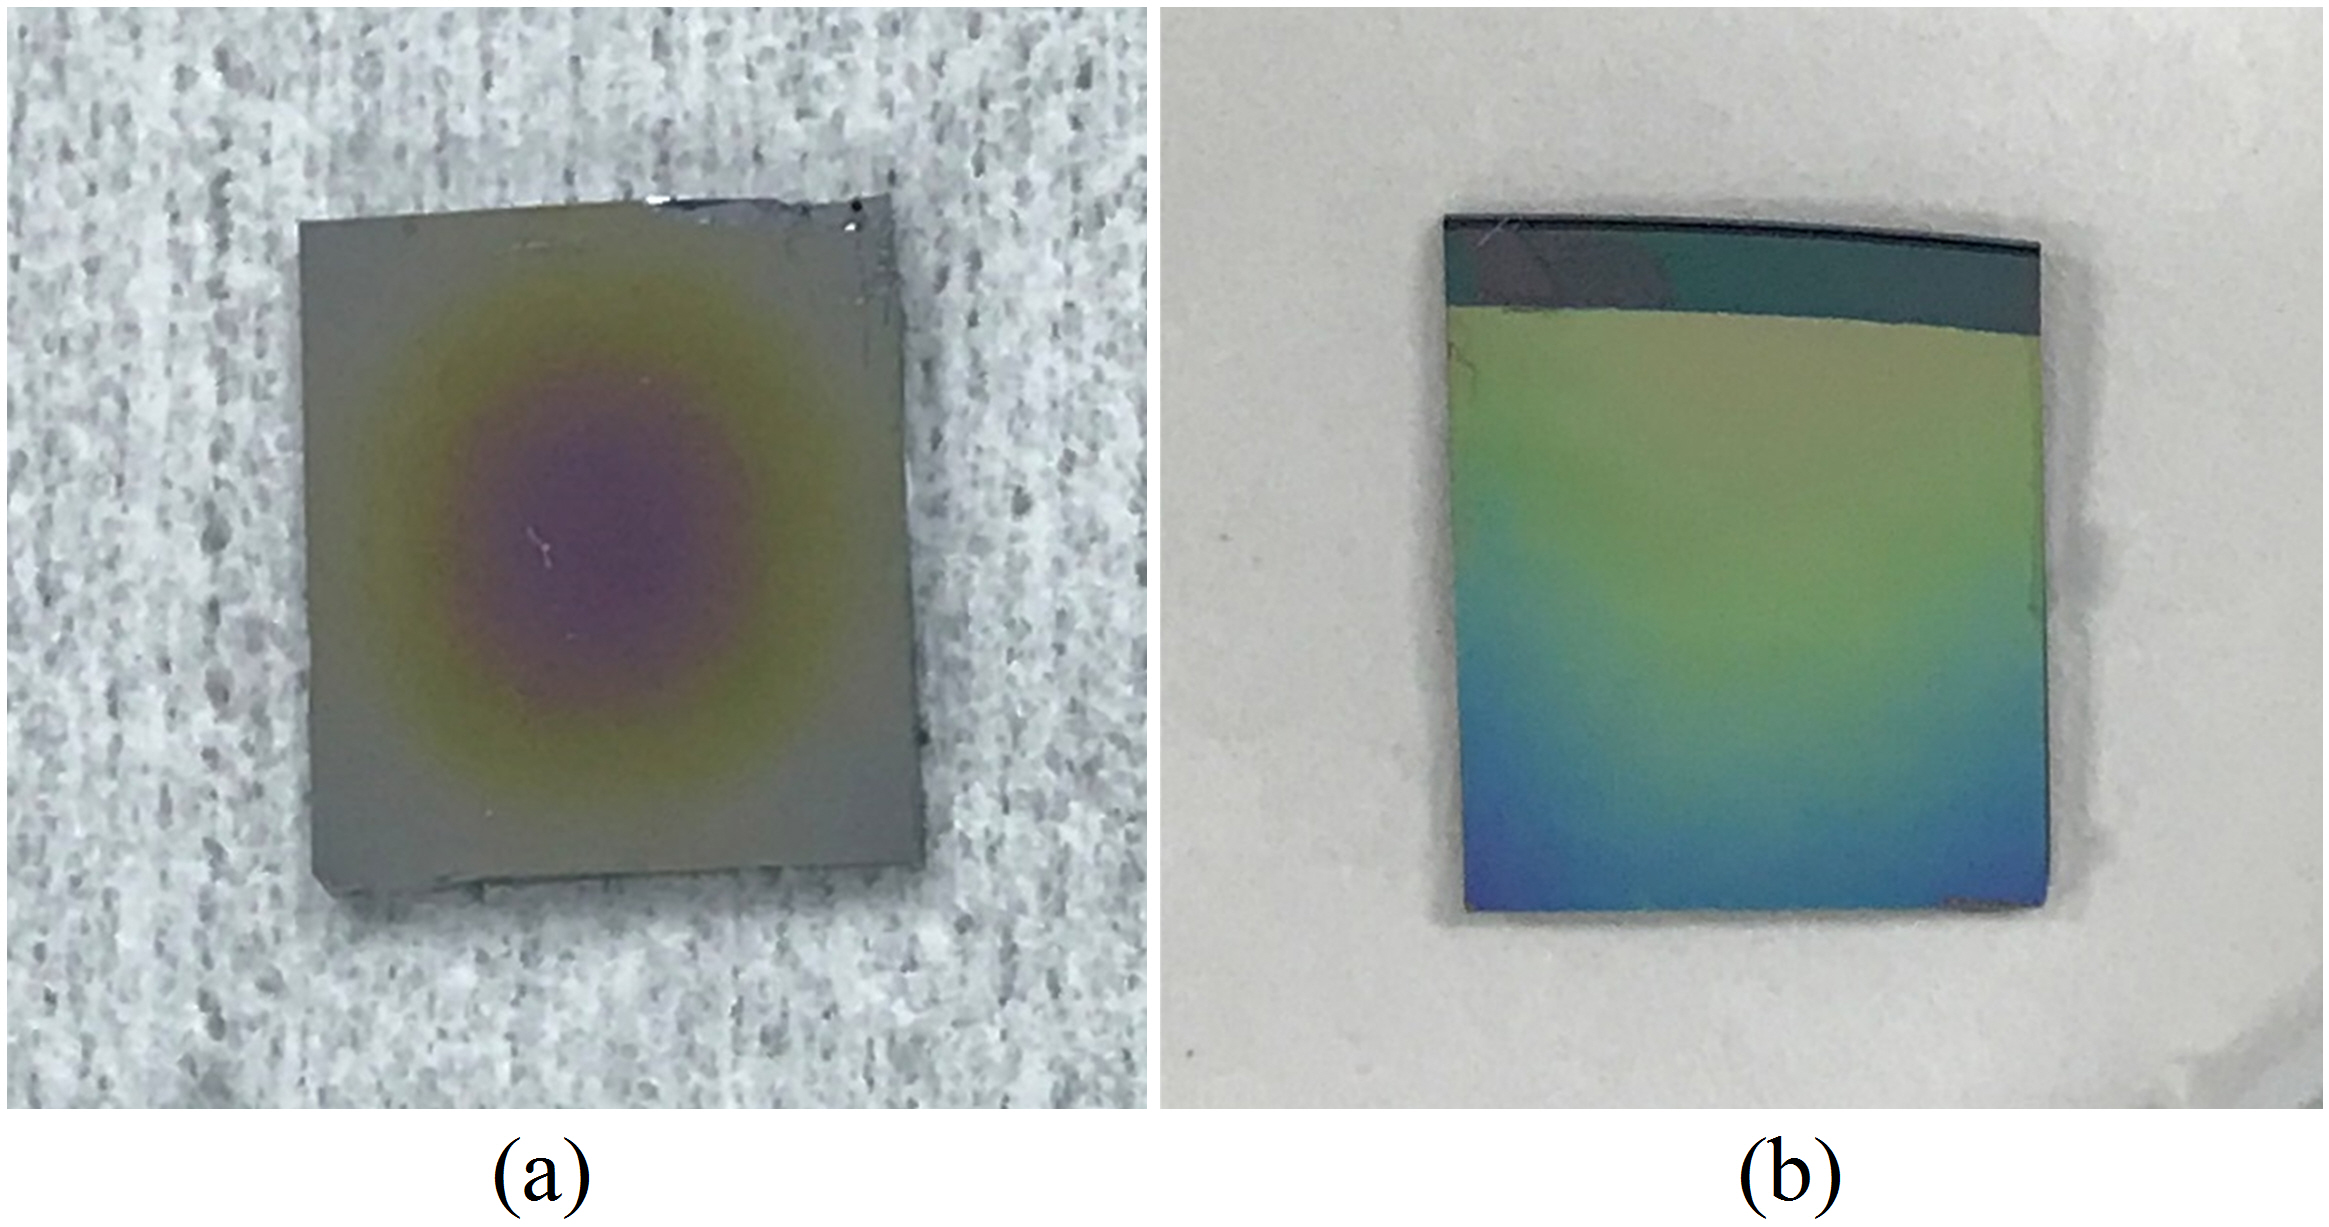
\includegraphics[width=12cm]{./Pictures/color_experiment.jpg}
	\captionsetup{justification=centering}
	\caption{ICP刻蚀之后的SOI芯片,(a)中心硅层厚度65~$nm$;(b)中心硅层厚度90~$nm$}
	\label{color_experiment}
\end{figure}

为了验证该方法的可靠性,我们利用SEM对SOI芯片的硅层厚度进行了测量作为标准值,然后让7名实验者利用SOIEtch软件,通过颜色比较法,读取对应SOI芯片的厚度,与标准值进行比较,所得结果如图\ref{color_experiment_measure}所示。从图中可以看到,当硅层厚度较大时,由于颜色变化比较缓慢,实验者利用颜色比较法测得的硅层厚度误差较大,且标准差也较大,这是由于颜色比较法是一种比较主观的方法,每个人对颜色相同的判断会有一定的差别,尤其是当颜色随厚度变化比较缓慢时;当硅层厚度较小时,由于颜色变化比较快速,实验者利用颜色比较法测得的硅层厚度误差较小,且标准差也较小。根据实验结果可以得知,当SOI芯片的硅层厚度小于120~$nm$时,利用颜色比较法测得的硅层厚度平均值与SEM测得的厚度值误差最大值为5.66~$nm$,考虑到SEM测得的硅层厚度也存在一定误差,有理由相信,该方法的实际误差将比5.66~$nm$更小。而且从图中还可以看到,当硅层厚度范围在40~\~{}80~$nm$时,通过颜色比较法测得的硅层厚度与SEM测得的厚度误差不超过2~$nm$,这已经足够满足大部分使用场景的需求。

\begin{figure}[htb]
	\centering
	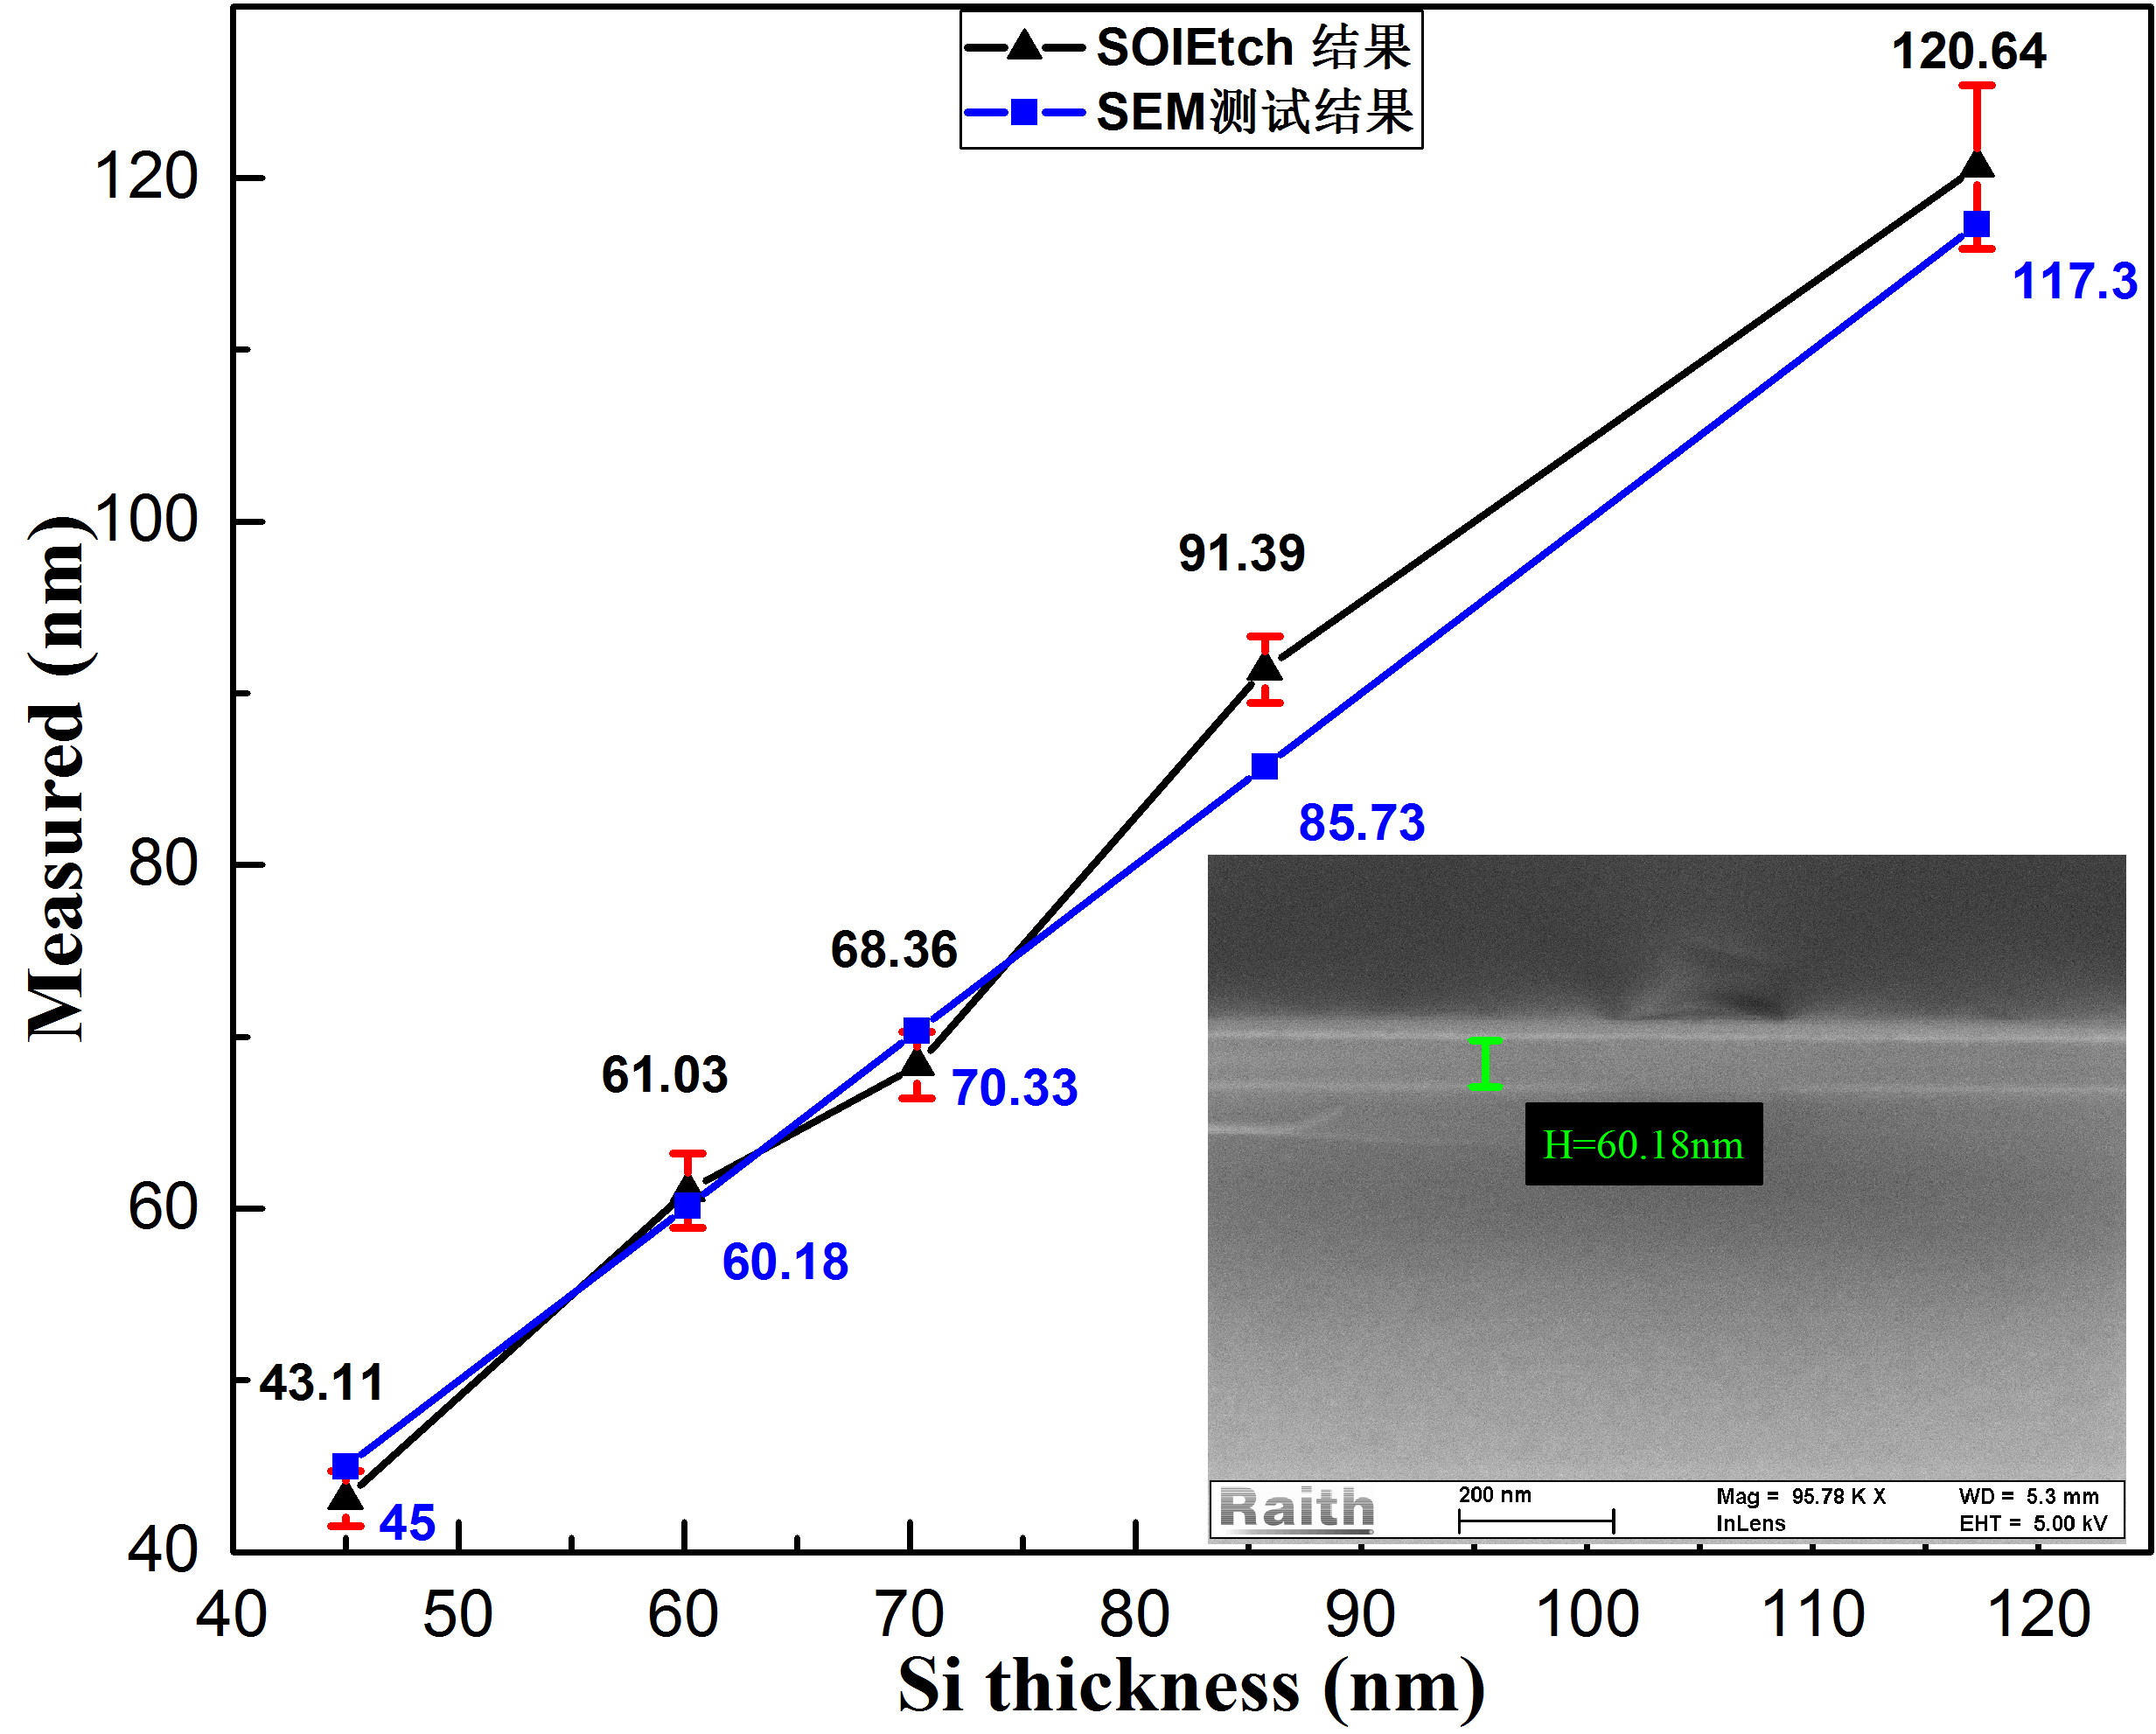
\includegraphics[width=13cm]{./Pictures/color_experiment_measure.jpg}
	\captionsetup{justification=centering}
	\caption{SEM与颜色比较法测得的硅层厚度比较,插图为SEM测试图}
	\label{color_experiment_measure}
\end{figure}

考虑到有的SOI芯片硅层较厚,我们用同样的方法计算了SOI芯片硅层厚度为0~\~{}~400~$nm$时的色谱图,如图\ref{color_400nm}所示。我们可以看到随着SOI芯片的硅层厚度越来越大,颜色的饱和度也越来越低,色调也只在红色和绿色之间转换,再利用颜色比较法来测定硅层厚度误差也将变大,此时该方法就不再适用。

\begin{figure}[htb]
	\centering
	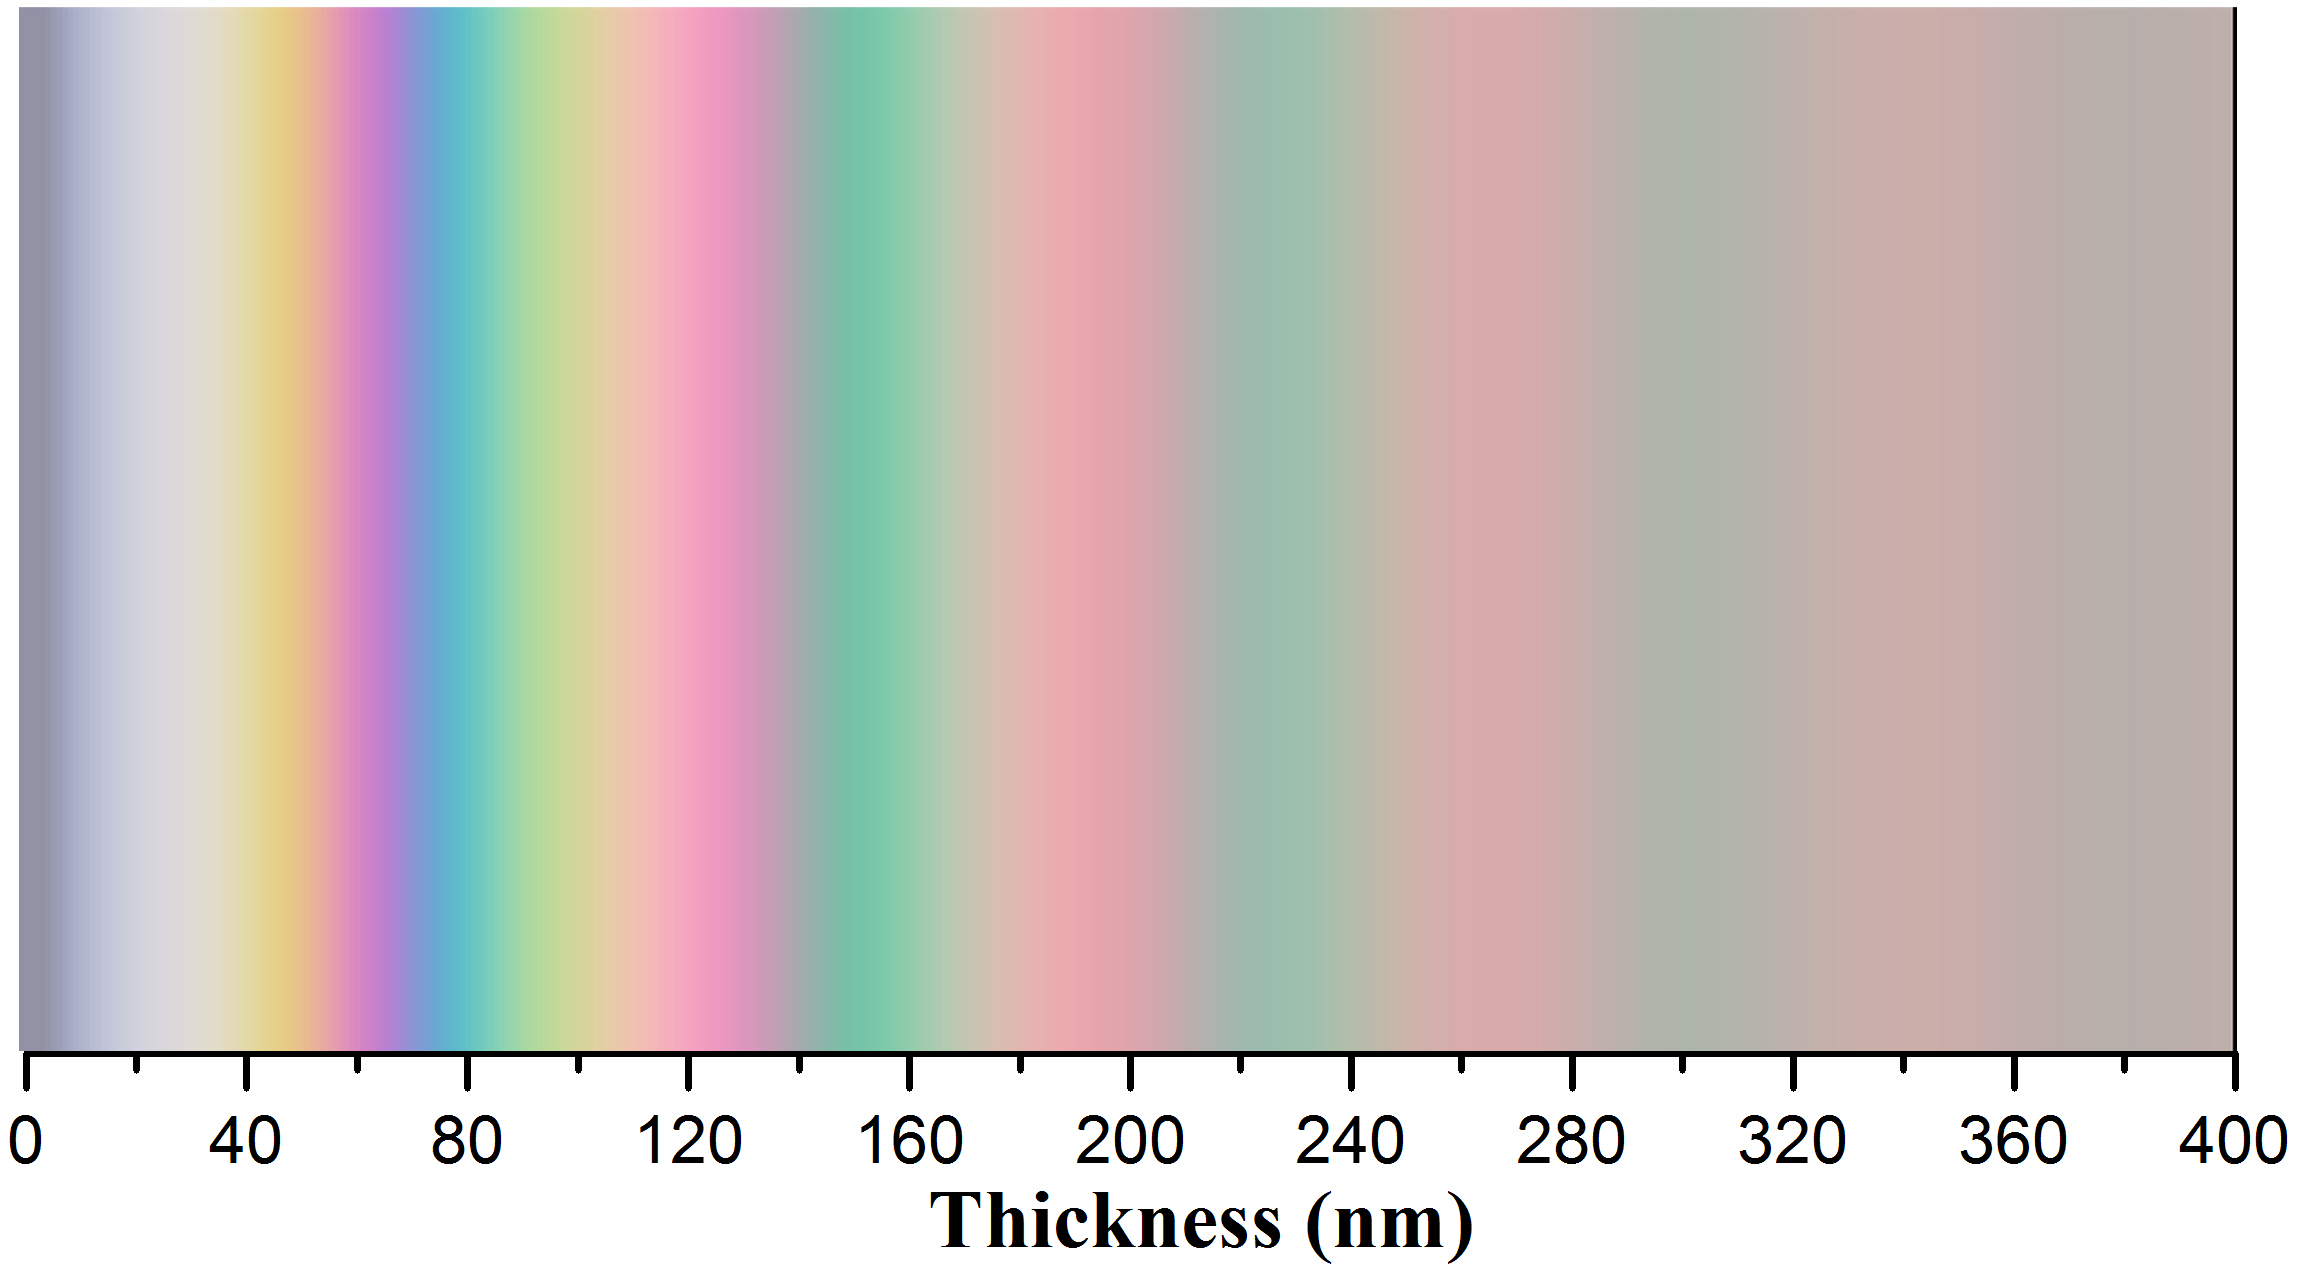
\includegraphics[width=13cm]{./Pictures/color_400nm.jpg}
	\captionsetup{justification=centering}
	\caption{0~\~{}~400~$nm$硅层厚度SOI芯片的色谱图}
	\label{color_400nm}
\end{figure}

\section{本章小结}

本章首先介绍了薄硅器件利用其低损耗等特性在集成器件领域的应用,以及目前获得薄硅的两种方法,ICP刻蚀法和热氧法。这两种方法都需要通过减薄现有SOI芯片的硅层厚度来实现,基于此本文提出了一种利用颜色比较法来帮助快速判断SOI芯片硅层厚度的方法。之后介绍了一些光度学与色度学的基础知识作为该颜色比较法的理论基础,然后通过数值仿真的方法计算得到SOI芯片不同硅层厚度的色谱图,给出了SOI芯片显示的颜色与硅层厚度之间的关系,并从理论上进行了分析。最后,专门开发了一款手机APP SOIEtch用来辅助颜色判断。经过实验测试,当硅层厚度小于120~$nm$时,颜色比较法测得的结果与SEM测得的结果相比较,可以达到较高的精度。









\chapter{硅基混合集成自脉冲DFB激光器}

\begin{comment}
\section{研究背景}
\subsection{光学时钟}
%\subsection{光学微波}
%\subsection{光互联}
自脉冲激光器作为光学时钟在光通信、光数据存储、光计算等方面具有非常重要的作用\cite{bornholdt2000self,feiste199418,barnsley1991all,renaudier200545,el2015all}。随着越来越多的光发射器和接收器用在短距离的光通信中,而硅基光子学在短距离通信中具有非常重要的作用,所以在硅波导上混合集成自脉冲激光器具有非常重要的意义。对于DFB自脉冲激光器,包括单段DFB自脉冲激光器\cite{wenzel1996mechanisms}和多段DFB自脉冲激光器\cite{mohrle1992gigahertz}。本章主要研究基于两段式DFB的自脉冲现象。两段式DFB的结构图如图\ref{laser_twosectiondfb}所示,DFB区域被分成两段,还有一段用来调整相位。
%\section{5G}
\begin{figure}[htb]
	\centering
	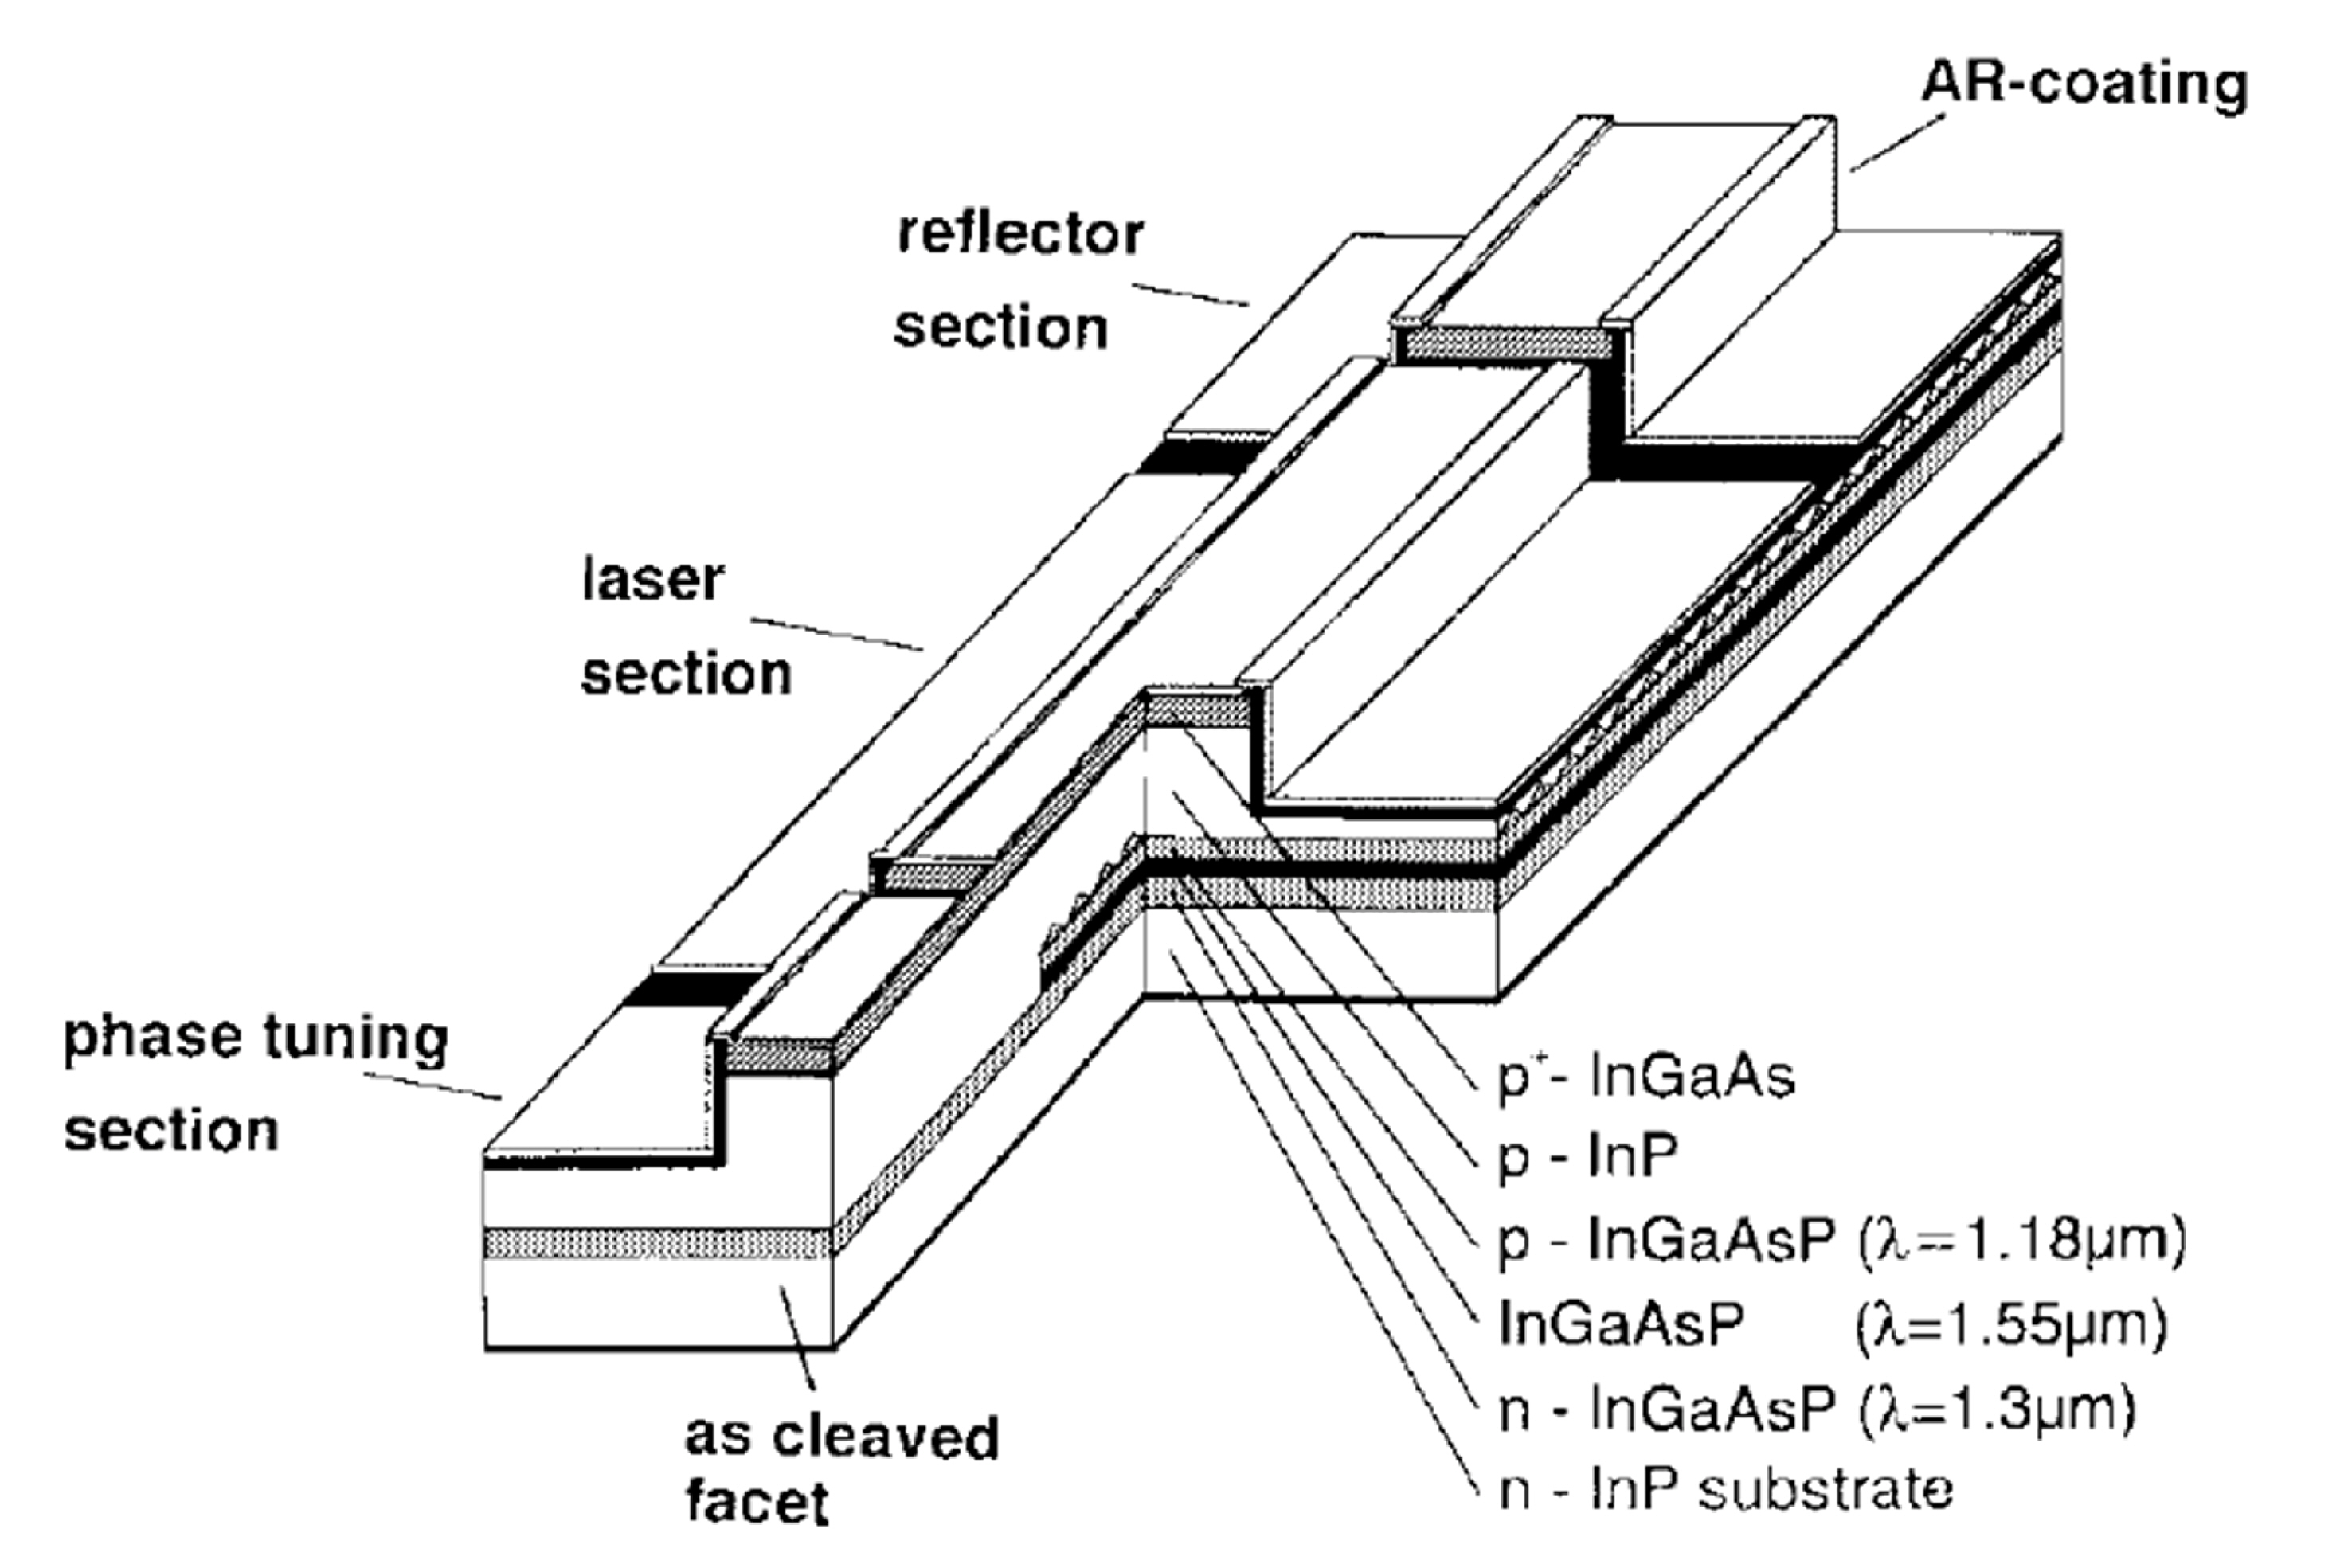
\includegraphics[width=14cm]{./Pictures/laser_twosectiondfb.jpg}
	\captionsetup{justification=centering}
	\caption{两段式DFB激光器\cite{sartorius1997dispersive}}
	\label{laser_twosectiondfb}
\end{figure}
\end{comment}

\section{自脉冲激光器的原理}
对于两段式DFB激光器来说,自脉冲形成的原理有如下三种\cite{sartorius1997dispersive}:

\begin{figure}[htb]
	\centering
	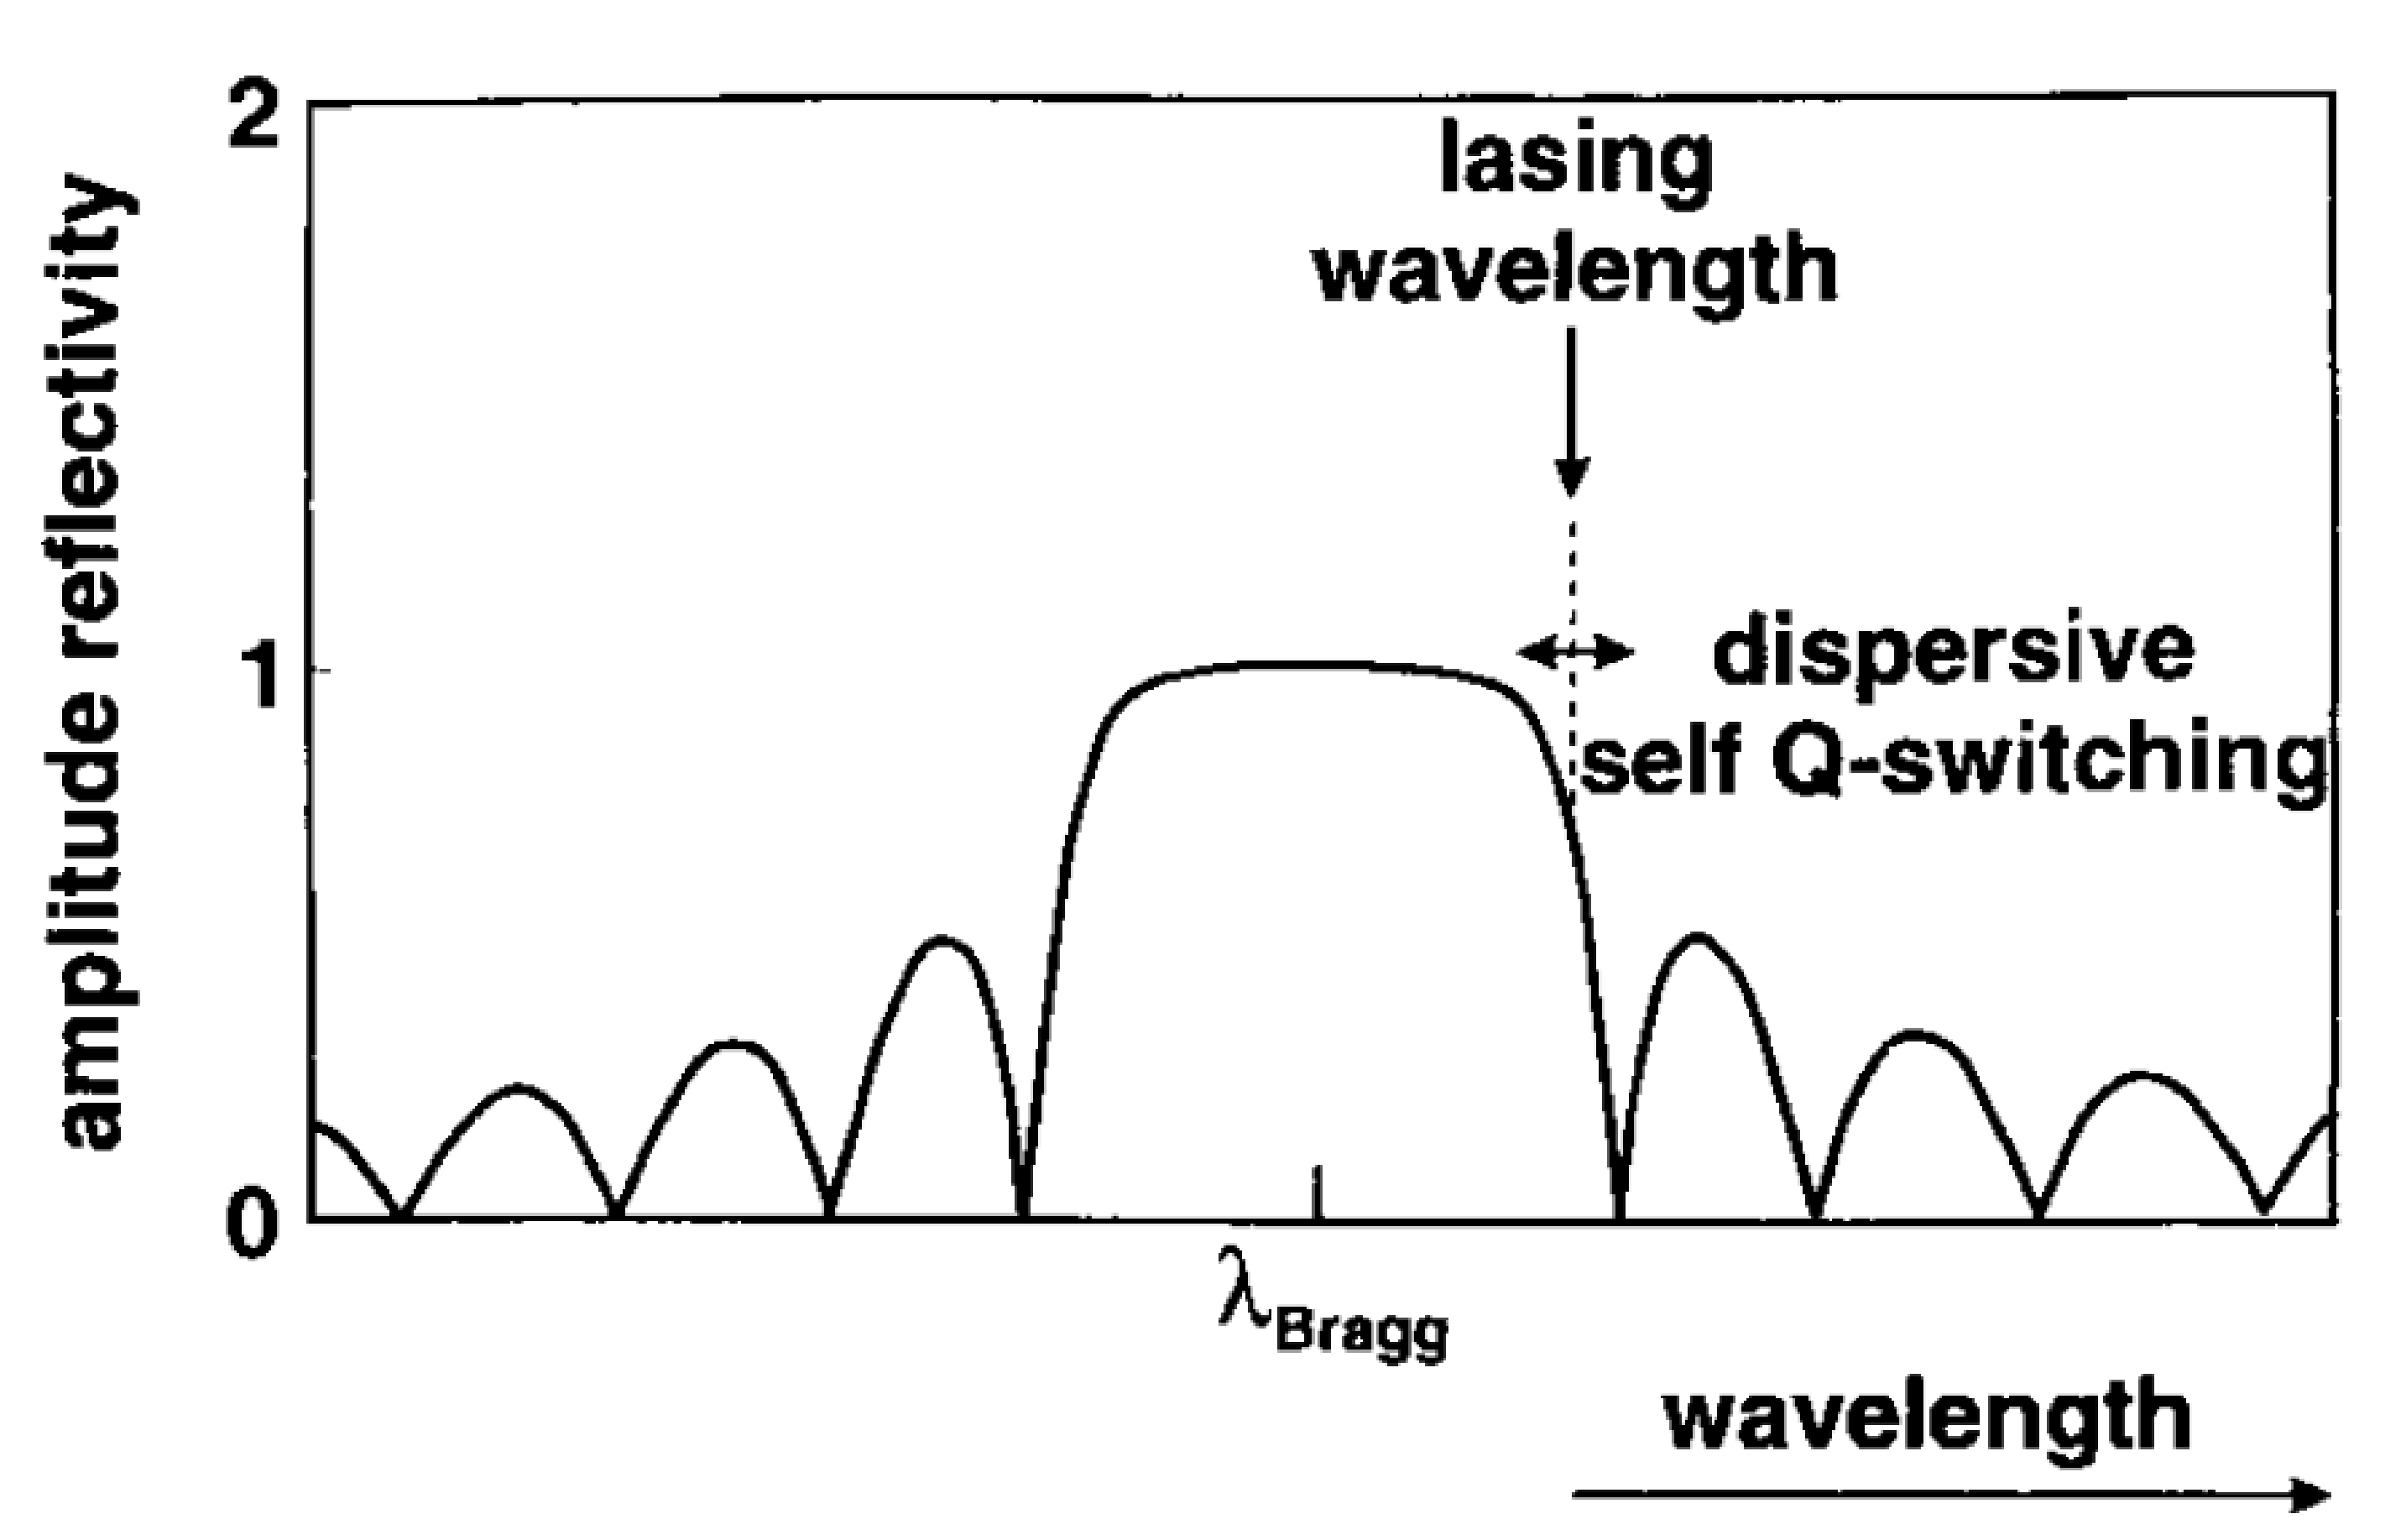
\includegraphics[width=12cm]{./Pictures/laser_selfQswitching.jpg}
	\captionsetup{justification=centering}
	\caption{色散自Q开关脉冲激光器的原理示意图\cite{sartorius1997dispersive}}
	\label{laser_selfQswitching}
\end{figure}

第一种是色散自调Q开关(dispersive self-Q-switching)产生自脉冲。其原理如图\ref{laser_selfQswitching}所示,其中双段式DFB激光器中的一段泵浦电流刚好使其工作在透明区域,即使其既没有增益,也没有损耗。在这种泵浦情况下,这段区域作为反射镜,需要利用的就是这个反射镜陡峭的反射谱。另一段DFB激光器的泵浦电流比较大,使其处于激发状态,且其发射波长刚好位于反射镜的右边的斜坡上。这样一来,这段激光器的阈值就会跟激射波长非常相关。当激光器处于激发状态时,载流子浓度下降,材料折射率上升,激光器的谐振波长就会往长波方向漂移,此时反射镜提供的反射率就会下降,激光器的阈值上升,激光不再出射;相反的,当激光不再出射,载流子浓度又开始上升,材料的折射率又会下降,使得谐振波长又往短波方向漂移,反射镜提供的反射率又会上升,激光器的阈值下降,激光又可以出射,如此周而往复,就形成了自脉冲的激光器。Bandelow等人\cite{bandelow1993theory}以单模为基础,利用传输波方程对该种类型的自脉冲激光器进行了研究。Marcenac等人\cite{marcenac1994distinction}则是用时域模型研究了类似的结构,都确认了该类型的自脉冲产生原因。总结起来,该种类型的自脉冲激光器有如下特征:

\begin{enumerate}
	\item 
	该种类型的自脉冲激光器都是单模的。
	\item 
	两段DFB激光器泵浦电流相差比较大。
	\item 
	自脉冲频率可以达到10GHz以上。
\end{enumerate}

第二种是空间烧孔效应产生自脉冲。当一个激光脉冲处于上升沿过程中,该模式的增益可能会由于空间烧孔效应下降,会出现跳模现象。当增益恢复之后,模式又会变回原来的模式,这个过程重复进行,就会出现自脉冲的现象。Lowery等人\cite{lowery1994improving}也观察到了自脉冲现象,他们将其归因于稳定的对称模式和不稳定的非对称模式之间由于空间烧孔效应引起的跳模。Phelan等人则认为除了空间烧孔效应,在多段DFB激光器中,载流子的互换也是产生自脉冲的原因之一。总结一下,对于空间烧孔效应引起的自脉冲激光器,有如下特征:

\begin{enumerate}
	\item 
	该种类型的自脉冲激光器都是多模的。
	\item 
	自脉冲频率一般小于5GHz。
\end{enumerate}

第三种是利用拍频产生自脉冲。这种机制由Wenzel等人\cite{wenzel1996mechanisms}提出。如果激光器的每一段都给予较高的泵浦电流,每一段都能产生一个激射波长,当这两个波长不一样时,就会出现拍频效应,拍频的频率正好是两束激光的频率之差,但这与两束不同的波长的激光相互干涉不一样,其中还包括了两段激光器之间光子与电子的互相耦合。这类自脉冲激光器的特征如下:

\begin{enumerate}
	\item 
	该种类型的自脉冲激光器都是多模的。
	\item 
	两段DFB激光器泵浦电流都比较大。
	\item 
	自脉冲频率可以达到100GHz以上。
\end{enumerate}

\section{硅基III-V混合集成技术}
如第一章所述,SOI平台上可以实现各种性能优异的无源器件,但是由于其为间接带隙材料,虽然科研人员在这个方向做了很多努力\cite{wirths2015lasing},要在其上制作电泵浦的激光器仍然困难重重。因此,人们非常希望能够将III-V材料和SOI结合来实现硅上的光源,这种方法可以同时利用硅和III-V材料各自的特点,从而可以在硅基平台上制作更加丰富的器件。

由于III-V材料与Si之间的晶格不匹配度达到8.1\%,在Si上直接外延生长会产生较多缺陷,故无法完美长出大面积的III-V外延层。虽然在第一章的介绍中已经介绍可以通过在Si上引入缓冲层或者限制缺陷扩展的结构,局部能够生长没有缺陷的外延层,实现了光泵浦激光器\cite{wang2015room},但是距离实现电泵浦激光器差距还很远。因此,现阶段研究人员主要采用键合的方式将III-V材料与SOI混合集成,实现在SOI上的电泵浦激光器,高速调制器、探测器和半导体光放大器\cite{liang2010hybrid,roelkens2010iii,liang2010recent,duan2014hybrid}。

\begin{figure}[htb]
	\centering
	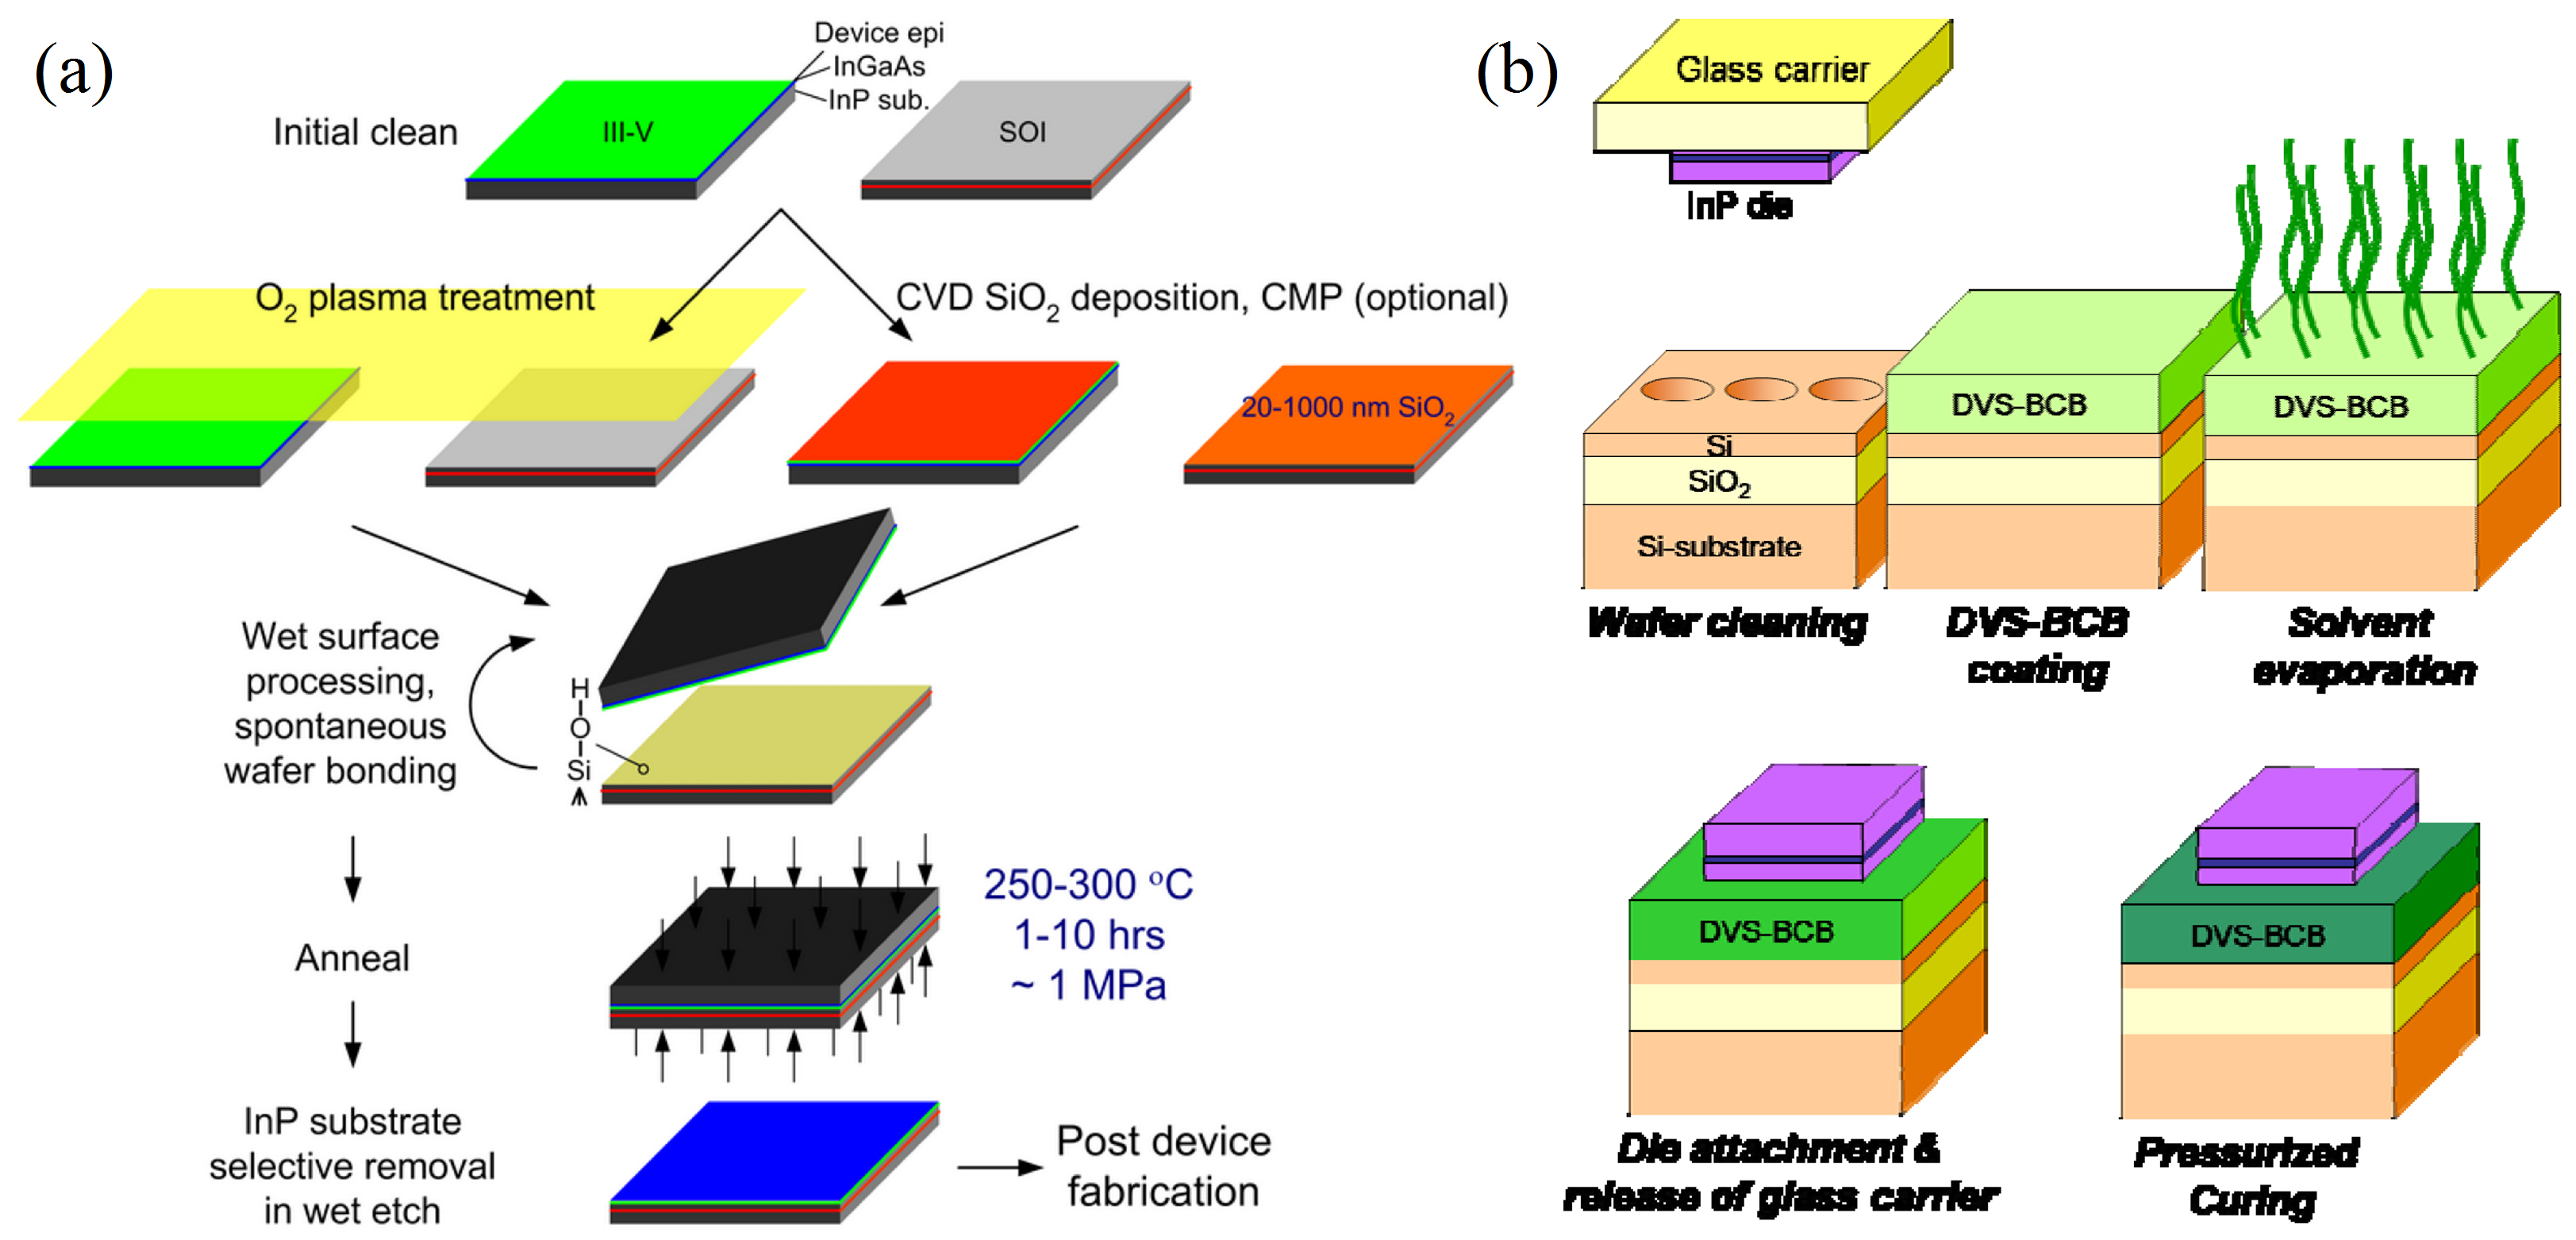
\includegraphics[width=14cm]{./Pictures/laser_bonding.jpg}
	\captionsetup{justification=centering}
	\caption{(a)III-V和SOI直接键合工艺流程示意图\cite{liang2010hybrid};(b)III-V和SOI粘贴键合工艺流程示意图\cite{liang2010hybrid}}
	\label{laser_bonding}
\end{figure}

目前,有两种比较常用的键合方式。一种是III-V芯片和SOI芯片通过O\SB{2}等离子体表面处理或者沉积SiO\SB{2}利用共价键直接键合的方式,具体工艺流程示意图如图\ref{laser_bonding}(a)所示。首先用BOE溶液去除InP芯片和SOI芯片表面的原生氧化层,获得干净疏水的表面。之后可以用O\SB{2}等离子体处理表面,使其产生约15 $nm$的等离子体氧化层,此时表面将变得非常光滑(RMS < 0.5 $nm$)且处于活化的状态。该过程中,O\SB{2}等离子体还起到了清洁晶片表面的作用,可以有效地去除表面的有机物。然后将InP芯片与SOI芯片贴合,在250~\~{}300 $^{\circ}$C、1 $MPa$的压力下进行退火处理,就可以将两者键合到一起。这种方法最早由瑞典的乌普萨拉大学的研究人员提出\cite{pasquariello2002plasma},后由美国加州大学圣塔芭芭拉分校(UCSB)的研究人员进一步优化\cite{liang2010hybrid},解决了键合表面会产生气体的问题。对于SiO\SB{2}共价键直接键合的方式,在第一步清洗完InP芯片与SOI芯片之后,在InP芯片表面通过PECVD长一层SiO\SB{2},在SOI芯片表面通过热氧长一层SiO\SB{2},之后通过化学机械腐蚀(chemical mechanical polishing, CMP)将表面的粗糙度下降到小于1 $nm$。然后可以通过稀释的标准RCA-1溶液在75 $^{\circ}$C下清洗10 $min$在表面形成Si-OH钝化层。之后的步骤则与用O\SB{2}等离子体处理表面直接建合法一样,通过贴合,加压退火,就可以将InP芯片与SOI芯片键合到一起。退火过程中发生的反应如公式\ref{bonding_1}和\ref{bonding_2}所示\cite{liang2010hybrid},其中M代表高电负性的金属(比如In, P):

\begin{equation}
\label{bonding_1}
\rm \ce{Si-OH} + \ce{M-OH} \rightarrow \ce{Si-O-M} +HOH(g)
\end{equation}

\begin{equation}
\label{bonding_2}
\rm Si + 2H_{2}O \rightarrow SiO_2 +2H_2(g)
\end{equation}

另一种键合的方式是III-V芯片和SOI芯片通过粘贴键合,其具体工艺流程示意图如图\ref{laser_bonding}(b)所示。首先用标准清洗溶液SC1(NH\SB{4}OH:H\SB{2}O\SB{2}:H\SB{2}O混合溶液)清洗SOI芯片,去除其表面的颗粒物并使其变成亲水性。对于III-V芯片,则是通过使用HCl和H\SB{2}SO\SB{4}:3H\SB{2}O\SB{2}:H\SB{2}O溶液分别去除InP和InGaAsP牺牲层来达到清洗的目的。将SOI芯片与III-V芯片清洗好之后,先在SOI芯片上旋涂一层增粘剂(AP-3000, Dow Chemicals),然后旋涂用来键合的粘贴剂。可以充当粘合剂的材料很多,比如PMMA,SU-8等,但是DVS-BCB(divinylsiloxane bis benzocyclobutene)相比其他材料,有更好的粘贴强度、热稳定性和抗腐蚀性能,其唯一的缺点只有热导率较低,故选择将其作为粘合剂材料。基于BCB的键合方法,主要由根特大学的研究人员开发\cite{roelkens2010iii}。旋涂BCB之后,将SOI芯片放于150~$^{\circ}$C的热板上烘烤1~$min$以去除BCB中的稀释用的溶剂——均三甲苯(mesitylene),这一步非常重要,否则容易在键合界面产生气泡。之后将III-V芯片有源层朝下倒扣到SOI芯片上,最后放入键合机中进行真空加压烘烤,烘烤温度为250~$^{\circ}$C。烘烤过程中,BCB单体会发生狄尔斯-阿尔德反应(Diels-Alder reaction)形成三维网状结构,反应示意图如图\ref{laser_bcb}所示。反应过程中无副产物生成,所以在键合界面不会生成气泡。

\begin{figure}[htb]
	\centering
	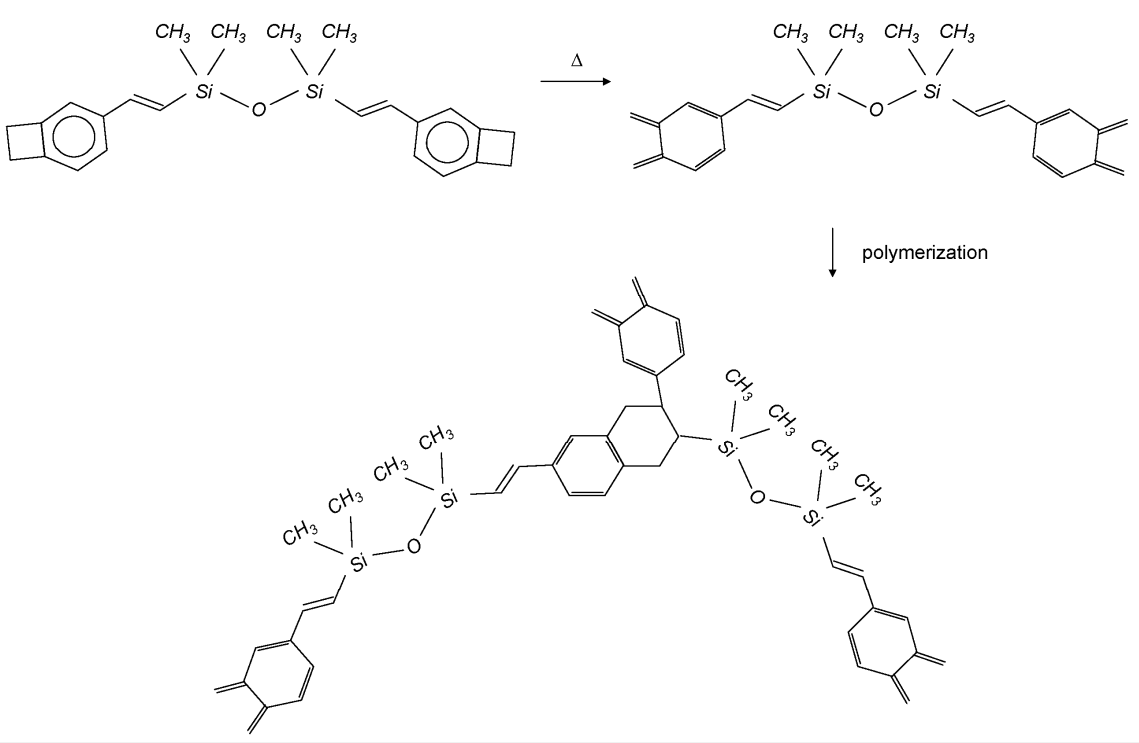
\includegraphics[width=11cm]{./Pictures/laser_bcb.png}
	\captionsetup{justification=centering}
	\caption{DVS-BCB单体聚合反应}
	\label{laser_bcb}
\end{figure}

虽然通过直接键合的方式,III-V芯片和SOI芯片之间的距离可以更近,更加方便光的耦合,但是其对III-V芯片和SOI芯片的表面粗糙度和洁净度要求非常高,工艺较为复杂。而通过BCB键合的方式,由于有中间层BCB的存在,降低了对III-V芯片和SOI芯片表面粗糙度和洁净度的要求\cite{roelkens2007heterogeneous},而且,通过将BCB稀释,也可以获得厚度小于100~$nm$的键合层,实现III-V波导和SOI波导之间光的耦合,故本文采用BCB粘贴键合的方式来制作混合集成的DFB激光器。

\section{器件的设计}

我们采用双段式DFB激光器的结构,通过拍频的方式实现自脉冲信号的产生,因为DFB激光器的单模性能较好,边摸抑制比高,故可以得到较为纯净的自脉冲信号。本文使用的多量子阱外延片的结构如表\ref{laser_material}所示,由台湾Landmark公司加工生产。

\begin{table}[htb]
	\zihao{5}
	\captionsetup{justification=centering}
	\caption{III-V外延片的材料参数}
	\label{laser_material}
	\centering
	\begin{tabular}[t]{|llll|}
		\hline
		\textbf{名称} & \textbf{材料组分} & \textbf{掺杂浓度 ($\pmb{cm^{-3}}$)} & \textbf{厚度($\pmb{nm}$)} \\
		\hline
		Sacrificial & InP & - &  200 \\
		\hline 
		Sacrificial & InGaAs & - &  200 \\
		\hline
		N cladding & InP & 1.00E18 & 190 \\
		\hline
		SCH & InGaAsP(Q1.17) & - & 100 \\
		\hline
		MQW well$\times$6 & InGaAsP(Q1.55) & - & 7 \\
		\hline
		MQW barrier$\times$7 & InGaAsP(Q1.17) & - & 9 \\
		\hline
		SCH & InGaAsP(Q1.17) & - & 100 \\
		\hline
		P cladding & InP & 5.00E17 & 500 \\
		\hline 
		P cladding & InP & 5.00E17->2.00E18 & 1000\\
		\hline
		Transition & InGaAsP(Q1.2) & >3.00E18 & 10\\
		\hline
		Transition & InGaAsP(Q1.4) & >3.00E18 & 10\\
		\hline
		P contact & InGaAsP & >1.5E19 & 200 \\
		\hline
		Sacrificial & InP & - & 200 \\
		\hline
		Stop etch & InGaAs & - & 200 \\
		\hline
		Substrate & InP & - & -\\
		\hline
	\end{tabular}
\end{table}

该外延片的PL谱测试结果如图\ref{laser_PL}所示,可以看到该外延片的光致荧光谱中心波长在1544.9 $nm$,增益带宽为63.0 $nm$。

\begin{figure}[htb]
	\centering
	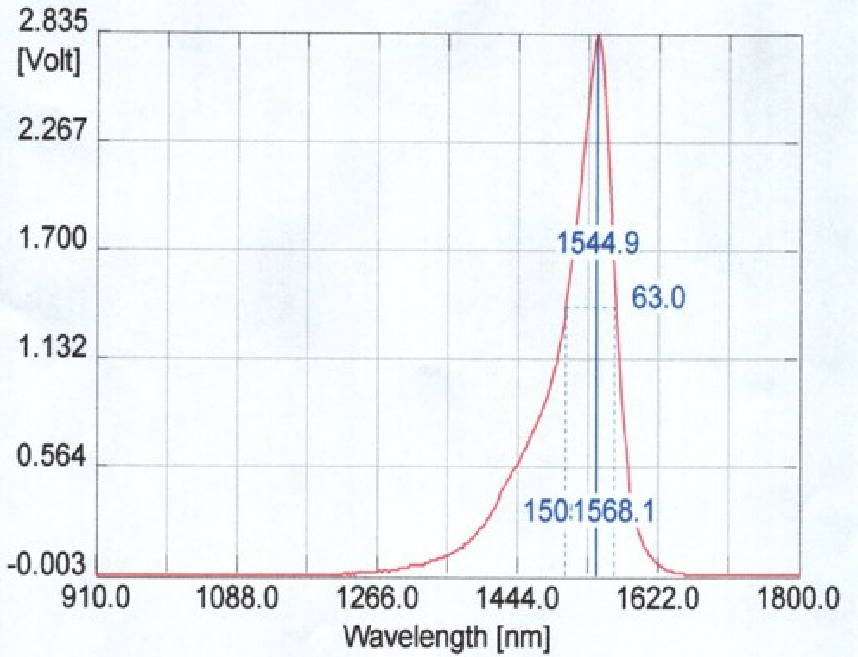
\includegraphics[width=10cm]{./Pictures/laser_PL.png}
	\captionsetup{justification=centering}
	\caption{表\ref{laser_material}所示的多量子阱外延片的光致荧光谱}
	\label{laser_PL}
\end{figure}

\begin{figure}[htb]
	\centering
	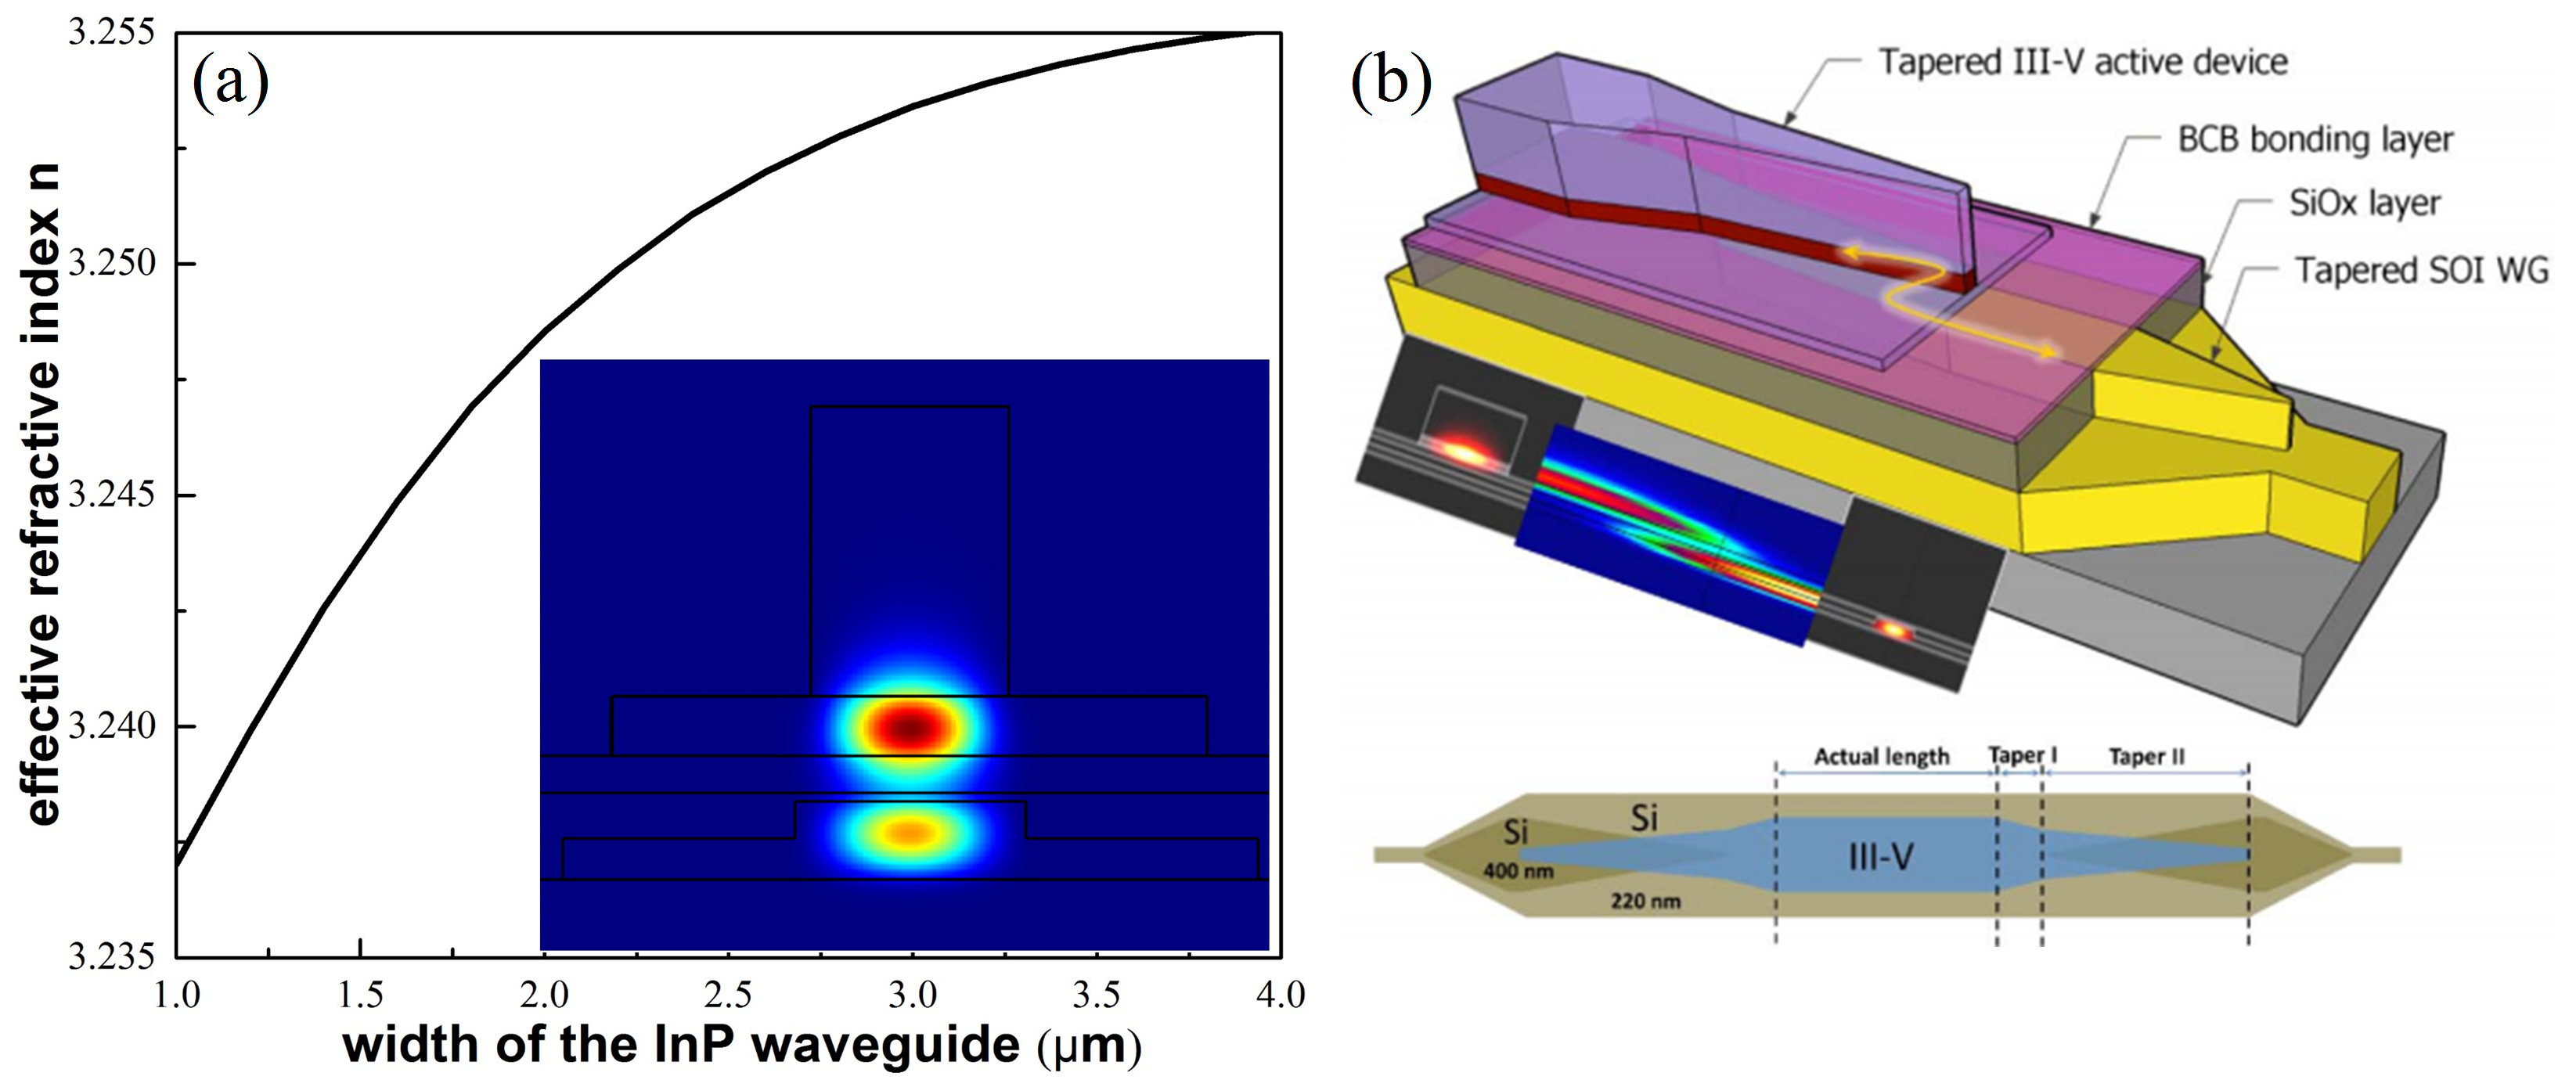
\includegraphics[width=14cm]{./Pictures/laser_modeandtaper.jpg}
	\captionsetup{justification=centering}
	\caption{(a)激光器的截面模式等效折射率随p-InP宽度变化图,插图为模式分布图;(b)两段式反向taper\cite{keyvaninia2013heterogeneously}}
	\label{laser_modeandtaper}
\end{figure}

III-V外延片中1.5 $\mu m$厚的P型InP层是为了让光传播模式远离高吸收的InGaAs层,减小III-V波导中的模式损耗。该多量子阱层由6层7~$nm$的InGaAsP势阱和7层9~$nm$的InGaAsP势垒组成。我们采用一阶光栅作为DFB激光器的光栅,将光栅制作在硅层厚度为400 $nm$的SOI芯片上,刻蚀深度为180 $nm$,周期$\Lambda$为246 $nm$,占空比为0.5,光栅宽度为3.5 $\mu m$,波导宽度为10.5 $\mu m$。III-V材料通过BCB与SOI键合,在光栅区域形成混合模式,部分能量在III-V材料中,部分能量在Si波导中。通过仿真得到如图\ref{laser_modeandtaper}(a)插图所示的截面模式图,该模式在量子阱中的限制因子为14.7\%,模式的限制因子越高,可以使激光器的阈值越低。激光器两边各通过一个反向锥形波导耦合器将光耦合到220~$nm$的硅波导中。锥形波导耦合器的结构用Keyvaninia等人采用的结构\cite{keyvaninia2013heterogeneously},如图\ref{laser_modeandtaper}(b)所示。该锥形波导耦合器分为两段且总长度为200 $\mu m$,第一段III-V波导从3~$\mu m$线性变到1~$\mu m$,长度为50~$\mu m$;第二段III-V波导从1~$\mu m$线性变化到600~$nm$,下面的脊型硅波导宽度从300~$nm$线性变化到2~$\mu m$,总长度为150~$\mu m$,该锥形波导耦合器可以实现高于90\%以上的耦合效率。

最后,我们设计的自脉冲DFB激光器如图\ref{laser_structure}所示,该激光器采用双段式设计,两边采用不一样的宽度是为了在同样的泵浦电流下,两段DFB激光器输出的波长错开一个阻带的宽度,从而可以同时用来研究色散自调Q开关和拍频产生自脉冲的现象。根据经验,该DFB激光器的阻带宽度约为4~\~{}5~$nm$左右,根据公式$2\Delta n_{eff}\Lambda = \Delta\lambda$计算得到$\Delta n_{eff}\approx 0.009$。根据\ref{laser_modeandtaper}(a)中等效折射率与p-InP波导宽度之间的关系,我们选取两段p-InP波导的宽度分别为2~$\mu m$和4~$\mu m$。p-InGaAs层在中间被刻蚀掉是为了进行电隔离,从而两段激光器可以注入不同的电流,倾斜的刻蚀可以尽量减少反射的光返回谐振腔内。产生的激光通过锥形波导耦合器耦合到硅波导,之后通过耦合光栅输出到光纤进行后续测试。

\begin{figure}[htb]
	\centering
	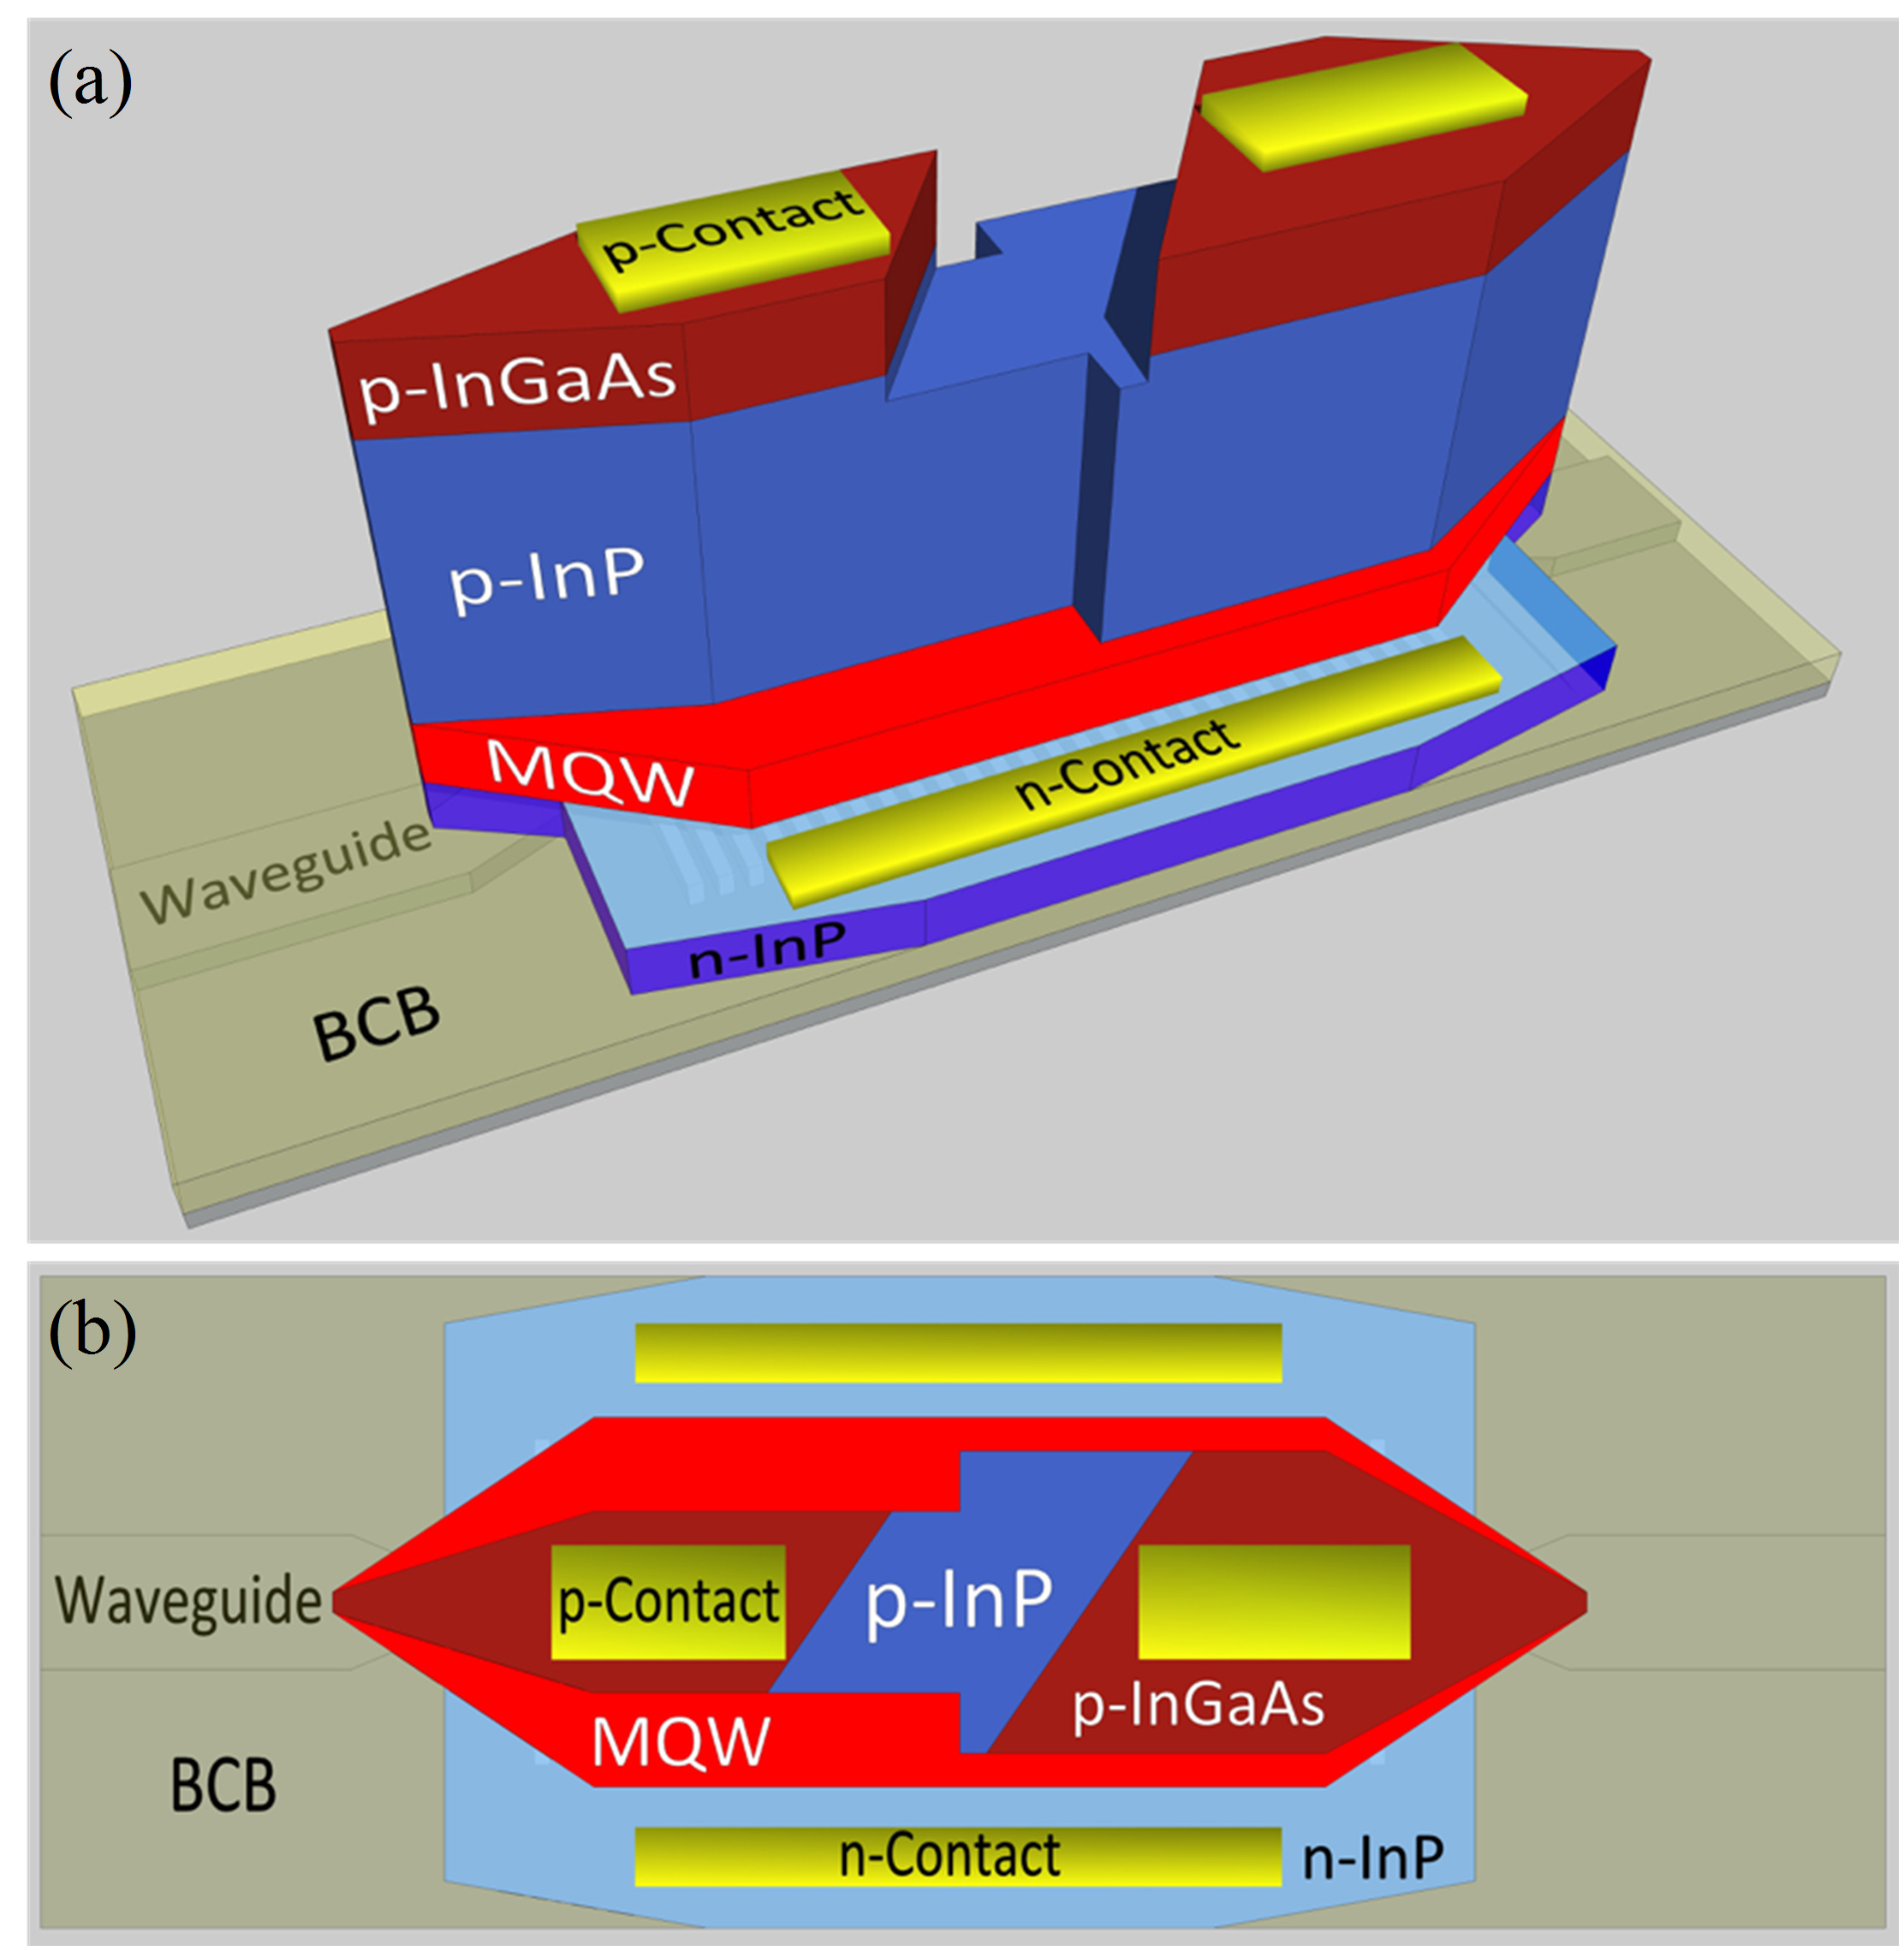
\includegraphics[width=12cm]{./Pictures/laser_structure.jpg}
	\captionsetup{justification=centering}
	\caption{双段式DFB激光器示意图,(a)~3D试图;(b)俯视图}
	\label{laser_structure}
\end{figure}

\section{制作工艺}

SOI芯片上的DFB光栅可以通过实验室电子束曝光之后使用ICP刻蚀完成或者委托半导体公司流片进行制作。用电子束曝光加ICP刻蚀的方法比较灵活,方便修改参数,加工周期短,但是波导损耗会较大且均一性较差。因为激光器对损耗相对比较敏感,实验室制作成功率不是特别高,如果采用EBL加工SOI芯片上的DFB光栅均一性无法保证。委托半导体公司进行流片,可以获得大量均一性好,损耗低的DFB一阶光栅,方便用来进行工艺摸索。我们委托Imec\cite{Imec}制作了SOI芯片上的DFB光栅。半导体公司流片时,会用100~$nm$左右的SiO\SB{2}进行表面平坦化处理,我们在进行键合时需要将该层去除,以增强硅波导与III-V波导之间的耦合。

下面介绍基于DVS-BCB粘贴键合的硅基混合集成DFB激光器制作工艺,主要分为两个部分。第一个部分是键合工艺;第二个部分是III-V波导与电极制作部分:
\begin{enumerate}[(1)]
	\item 
	从流片回来的SOI大晶圆上解理需要键合的芯片,为了方便操作,大小可以选取为2.5~$cm$~$\times$~2.5~$cm$,解理时需使所需要的DFB光栅处于芯片的中央位置,这样在键合时,III-V芯片位于SOI芯片的中央位置。解理时可以在表面旋涂一层光刻胶进行保护,防止解理产生的碎片划伤芯片表面。用丙酮、异丙醇清洗之后,再缓冲HF腐蚀液(buffered HF, BHF)去掉表面用于平坦化的SiO\SB{2}。
	\item 
	解理合适大小的III-V芯片,一般使其比SOI芯片上的DFB光栅区域边长大1~$mm$左右就已足够。用丙酮去除其表面用来保护的光刻胶,之后用HCl:H\SB{2}O=1:1的溶液去除InP牺牲层,再用食人鱼溶液H\SB{2}SO\SB{4}:H\SB{2}O\SB{2}:H\SB{2}O=1:1:18去除InGaAs牺牲层,可通过观察颜色来确定牺牲层是否去除干净。
	\item 
	为了增加III-V与BCB的粘附性,键合之前需要在III-V芯片上表面用PECVD长一层5~$nm$左右的SiO\SB{2}。
	\item 
	将SOI芯片与III-V芯片在150$^{\circ}$C热板上烘烤去水汽,然后在SOI芯片上旋涂BCB:均三甲苯(Mesatylane)=1:8的溶液,参数为500~rpm~5~$s$,3000~rpm~40~$s$。将匀好BCB的SOI芯片在150~$^{\circ}$C热板上烘烤10\~{}20~$min$,将溶剂均三甲苯挥发掉,防止键合时产生气泡。之后将热板调成20~$^{\circ}$C,当热板冷却到70~$^{\circ}$C时,将芯片取下,放于键合机的石英载玻片上准备键合。然后用镊子将III-V芯片倒扣到SOI芯片上,此步需要手工完成,并借助显微镜确定III-V芯片全部覆盖了SOI芯片上的DFB光栅。为了之后湿法腐蚀的III-V波导形成倒梯形的结构,使得模式可以更好的限制在多量子阱层中,III-V芯片的[011]晶向需要对准SOI芯片上的波导方向。
	\item 
	利用商用键合机S\.{U}SS MicroTec ELAN CB6L进行键合,由于该键合机适用于键合4英寸的芯片,而我们的芯片尺寸较小,因此我们需要将手工键合的芯片夹在两片4英寸的石英载玻片之间,如图\ref{laser_bonder}(a)所示。随后,我们将其放入键合机内进行键合,键合机会在真空环境下进行键合,这可以帮助将III-V芯片与SOI芯片之间的空气排除干净。键合机内的温度和压力变化曲线如图\ref{laser_bonder}(b)所示,当温度上升到150~$^{\circ}$C时,BCB还具有一定的流动性,这时加入200\~{}400~$KPa$的压力可以减小BCB的厚度,同时可以更好地填充III-V芯片与SOI芯片之间的缝隙,使得键合的强度更强。当温度高于180~$^{\circ}$C后,压力被撤去,以防BCB在高温玻璃化时产生较大的应力。键合完成后的芯片如图\ref{laser_bonder}(c)所示。
	\begin{figure}[htb]
		\centering
		\includegraphics[width=15cm]{./Pictures/laser_bonder.jpg}
		\captionsetup{justification=centering}
		\caption{(a)夹在两片4英寸石英载玻片之间的SOI芯片和III-V芯片;(b)键合机键合过程中温度和压力随时间变化曲线;(c)键合完成后的芯片}
		\label{laser_bonder}
	\end{figure}
	\item 
	用HCL:H\SB{2}O=3:1的溶液加热到40~$^{\circ}$C去除III-V芯片的衬底InP,加热是为了加快去除衬底的速度。当不再有气泡产生时,说明衬底已经去除干净,总时间大约为15\~{}25~$min$。有时如果键合的质量不够好,去除衬底之后部分III-V芯片就会脱落,如图\ref{laser_sub_removal}(a)所示,这是由于去除衬底之后III-V芯片厚度只有2.615~$\mu m$,如有应力存在,较容易破裂。但如果掉落的面积不大,有的DFB光栅上依然有III-V芯片,则实验可以继续。\ref{laser_sub_removal}(b)所示为去除衬底过程中的侧向腐蚀现象,HCl通过边缘腐蚀InP,这可以通过在III-V芯片四周涂抹一层光刻胶解决,但是一般只要在解理III-V芯片时稍微留点余量,则问题并不大,可以看到侧向腐蚀最大处也不过400~$\mu m$不到。
	\begin{figure}[htb]
		\centering
		\includegraphics[width=14cm]{./Pictures/laser_sub_removal.jpg}
		\captionsetup{justification=centering}
		\caption{(a)因键合质量不好部分III-V芯片脱落;(b)去除衬底过程中的侧向腐蚀现象}
		\label{laser_sub_removal}
	\end{figure}
	\item 
	用食人鱼溶液H\SB{2}SO\SB{4}:H\SB{2}O\SB{2}:H\SB{2}O=1:1:18去除InGaAs牺牲层,用纯盐酸去除InP牺牲层,这里同第(2)步一样可以通过颜色变化来判断牺牲层是否去除干净。去除完牺牲层后芯片示意图如图\ref{laser_fab}(a)所示。
	
	\begin{figure}[htb]
		\centering
		\includegraphics[width=15cm]{./Pictures/laser_fab.jpg}
		\captionsetup{justification=centering}
		\caption{硅基III-V混合集成自脉冲DFB激光器工艺流程示意图,(a)\~{}(l)展示了不同步骤下的波导截面图}
		\label{laser_fab}
	\end{figure}

	\item 
	从这一步开始开始制作III-V波导,首先在p-InGaAs上沉积5~$nm$~SiO\SB{2}和200~$nm$~SiN作为掩模,芯片示意图如图\ref{laser_fab}(b)所示。
	\item 
	利用SOI芯片上的套刻标记,光刻制作p-InGaAs层的结构。先将芯片放于120 $^{\circ}$C的热板上去水汽5~$min$以上,然后将芯片放置于常温金属块上冷却之后,旋涂增粘剂Ti Prime,4000 rpm 40~$s$,之后120 $^{\circ}$C烘烤3 $min$,以增强芯片与光刻胶的粘附性。因为该层图案宽度较小,最窄处只有750~$nm$,如果粘附性不好,光刻胶就很容易掉落。烘烤之后旋涂高分辨率光刻胶MIR 701,4000~rpm 40~$s$,之后100~$^{\circ}$C烘烤1~$min$~20~$s$。接下去进行接触式曝光,曝光时间为120 $s$,光刻机采用S\.{U}SS MicroTec MA6,曝光波长为320~$nm$,功率为325~$W$,曝光时间为120~$s$。曝光完成需要后烘,110~$^{\circ}$C烘烤1~$min$。之后用MIF显影液显影,通过芯片表面的彩色条纹全部退去判断显影是否完成,用显微镜检查曝光质量,如果p-InGaAs层颜色均匀,说明曝光质量可以接受。最后用反应离子刻蚀机(Reactive Ion Etching, RIE)刻蚀SiN,刻蚀时间为2~$min$~30~$s$。刻蚀完成后用丙酮,异丙醇,水清洗刻蚀完之后的芯片,去除残留的光刻胶,此时的芯片示意图如图\ref{laser_fab}(c)所示。
	\item 
	用ICP刻蚀InGaAs,刻蚀气体为CH\SB{4}和H\SB{2},采用多个周期刻蚀,每个周期刻蚀深度约为50~$nm$。通过台阶仪判断刻蚀终点,刻蚀深度要大于220 $nm$以保证InGaAs已经刻蚀完,否则会造成下一步湿法腐蚀无法进行,此时芯片示意图如图\ref{laser_fab}(d)所示。
	\item
	用HCl:H\SB{2}O=1:1溶液湿法腐蚀InP,这一步中可以使用摇床加快腐蚀速度。由于InP的腐蚀有晶向特性,故最终会形成倒梯形结构,使得模式能够更好的限制在多量子阱层,降低激光器的阈值电流。如果在键合的时候III-V芯片的晶向放置错误,这一步就会形成正梯形的结构,模式在有源区中的限制因子就会降低,使得激光器的阈值电流增大。该步通过分步多次腐蚀划台阶仪的方法来确定腐蚀终点,越接近终点,腐蚀间隔取的越短,当两次腐蚀深度不再增加的时候,即可判断已经腐蚀到多量子阱层。此步完成之后的芯片示意图如图\ref{laser_fab}(e)所示。
	\item 
	用PECVD沉积200~$nm$左右的SiN保护InP侧壁和作为制作多量子阱层的掩模,此时芯片示意图如图\ref{laser_fab}(f)所示。
	\item 
	光刻制作多量子阱层的结构。该步依然采用Ti Prime与MIR 701,此时将MIR 701的转速降为3000 rpm,其他参数与(9)相同,用RIE刻蚀SiN,ICP刻蚀多量子阱层。我们采用宽度为9~$\mu m$的量子阱宽度,这样可以减小ICP刻蚀造成的表面缺陷态对载流子的影响。此时芯片示意图如图\ref{laser_fab}(g)所示。
	\item 
	光刻制作n金属接触(n-contact)结构。此步采用光刻胶Ti 35E,匀胶参数为3000 rpm 40 $s$,100 $^{\circ}$C烘烤3 $min$,曝光时间为55 $s$,等10分钟后,再125 $^{\circ}$C烘烤2 $min$,之后空曝185~$s$做图像反转,用AZ400:H\SB{2}O = 1:3显影1 $min$ 20 $s$。然后用RIE刻蚀几秒钟去除可能残留的光刻胶,再在H\SB{2}SO\SB{4}:H\SB{2}O\SB{2}:H\SB{2}O=1:1:20溶液中快速浸5 $s$去除可能存在的氧化层,此步需要在蒸镀之前尽量短的时间内做以避免再次被氧化。最后蒸镀金属Ni:Ge:Au= 30~$nm$:20~$nm$:50~$nm$,利用剥离工艺(lift-off)去除多余金属。此时芯片示意图如图\ref{laser_fab}(h)所示。
	\item 
	光刻制作n-InP层上的结构。先旋涂Ti Prime,参数与(9)中相同,然后旋涂光刻胶AZ 9260,3000~rpm 40~$s$,之后100 $^{\circ}$C烘烤40~$s$,曝光200~$s$。曝光之后用AZ400:H\SB{2}O = 1:2显影2~$min$~30~$s$。用HCl:H\SB{2}O = 1:1溶液将没有被光刻胶保护的n-InP腐蚀掉,此步可以通过颜色和台阶仪共同确定腐蚀终点,如图\ref{laser_island}所示。再用丙酮,异丙醇去掉光刻胶,沉积600~$nm$~SiN做钝化处理。
	\begin{figure}[htb]
		\centering
		\includegraphics[width=14cm]{./Pictures/laser_island.jpg}
		\captionsetup{justification=centering}
		\caption{(a)~n-InP还未腐蚀干净;(b)~n-InP已经腐蚀干净}
		\label{laser_island}
	\end{figure}
	\item 
	旋涂BCB 3022-57做平坦化处理,转速2000 rpm 40~$s$,以得到较厚的BCB,超过III-V波导的高度。然后用烘箱280 $^{\circ}$C烘烤2小时使其玻璃化,之后用来承载电极。此时芯片示意图如图\ref{laser_fab}(i)所示。
	\item 
	使用RIE回刻BCB至InGaAs上的SiN处,通过台阶仪判断刻蚀终点。然后RIE换配方刻蚀完InGaAs上的SiN,光刻制作InGaAs中间的刻蚀部分,用光刻胶Ti 35E,参数与(14)中相同,然后ICP刻蚀InGaAs,刻蚀深度需要保证大于220~$nm$,使得两段电极分离。
	\begin{figure}[htb]
		\centering
		\includegraphics[width=14cm]{./Pictures/laser_cut.jpg}
		\captionsetup{justification=centering}
		\caption{p-contact中间的电隔离区域}
		\label{laser_cut}
	\end{figure}
	\item 
	光刻制作p金属接触结构(p-contact)的结构,采用Ti Prime和光刻胶Ti 35E,参数与(14)中相同,曝光之后反转。显影之后,蒸镀前利用RIE刻蚀30~$s$去掉残留的光刻胶,用H\SB{2}SO\SB{4}:H\SB{2}O\SB{2}:H\SB{2}O=1:1:20溶液浸泡5~$s$去除氧化层。蒸镀Ti:Au=40~$nm$:150~$nm$,利用剥离工艺去除多余的金属。此时芯片示意图如图\ref{laser_fab}(j)所示,在显微镜下如图\ref{laser_cut}所示。
	\item
	使用RIE刻蚀BCB在n接触层上方开窗口,采用光刻胶Ti 35E光刻胶,参数与(14)中相同,用RIE刻蚀BCB和SiN,露出n接触层金属,此处可以用台阶仪来判断刻蚀终点,刻蚀完成芯片示意图如图\ref{laser_fab}(k)所示。
	\item 
	用氧气等离子体清洗电极表面,光刻最后的电极结构,采用光刻胶Ti 35E,参数与(14)中相同。利用RIE刻蚀30~$s$去掉残留的光刻胶,蒸镀Ti:Au=40~$nm$:800~$nm$,用剥离工艺去除多余的金属,完成器件的制作,芯片示意图如图\ref{laser_fab}(l)所示。
\end{enumerate}



最终制作完成的硅基混合集成自脉冲DFB激光器如图\ref{laser_fabricationresult}(a)所示。使用FIB观察激光器的截面图如图\ref{laser_fabricationresult}(b)所示,几乎无法看到BCB键合层,说明BCB的厚度非常薄。从图中还可以看出光刻的套刻偏差在200~$nm$左右。

\begin{figure}[htb]
	\centering
	\includegraphics[width=15cm]{./Pictures/laser_fabricationresult.jpg}
	\captionsetup{justification=centering}
	\caption{(a)制作完成的硅基混合集成自脉冲DFB激光器芯片;(b)激光器截面SEM图,靠近III-V波导锥形结构尖端处}
	\label{laser_fabricationresult}
\end{figure}


\section{自脉冲激光器的静态性能测试}

\subsection{金属电极退火}

制作完激光器之后,首先需要进行I-V曲线测试,以判断器件是否能够正常工作。本文所制作该的自脉冲激光器,整体是个PIN结构,所以其I-V曲线也是标准的二极管响应曲线。当电极制作完成后,如果接触电阻过大,可以对器件进行快速退火处理,将金属电极与p接触层、n接触层的温度瞬间加热到极高的温度,改善它们之间的接触。常用的快速退火方法有脉冲激光退火与脉冲电子退火,本文为了方便采用的是电压快速退火法。通过在电极上加载一个比较高的电压,利用电阻产生的焦耳热直接对电极进行退火,可以对单个器件进行退火,而且本来对每个器件测试过程中就需要加载电压,故该方法适合实验中使用。该方法的缺点是如果电流太大,有可能将电极烧坏,故在退火时有需要限制最大电流的大小。

\begin{figure}[htb]
	\centering
	\includegraphics[width=12cm]{./Pictures/laser_annealing.jpg}
	\captionsetup{justification=centering}
	\caption{退火前与退火后自脉冲激光器的I-V曲线}
	\label{laser_annealing}
\end{figure}

图\ref{laser_annealing}中退火前的曲线是是将电流从0 $mA$逐渐增加到100 $mA$获得的,可以看到此时电压增加也比较快,但当电流增加到60 $mA$时,可以看到IV曲线中一个较明显的陡坡,对应着此时电阻瞬间较小,从而说明退火成功。当我们重新测试该器件的IV曲线时,可以发现退火后的IV曲线整体在退火前的IV曲线上方,说明退火之后的器件总电阻已经减小,该器件减小之后的总电阻在8.3 $\Omega$左右。 

\subsection{IV和PV曲线}

\begin{figure}[htb]
	\centering
	\includegraphics[width=15cm]{./Pictures/laser_IV.jpg}
	\captionsetup{justification=centering}
	\caption{两段式DFB激光器的IV响应曲线,(a)右段激光器的IV响应曲线;(b)左段激光器的IV响应曲线}
	\label{laser_IV}
\end{figure}

图\ref{laser_IV}给出了制作的某个激光器左右两段的IV响应曲线,测试温度为15$^{\circ}$C。该DFB激光器III-V波导由两段组成,总长度为900 $\mu m$。左边一段由长度为250~$\mu m$,宽度为2.5 $\mu m$的直波导和长度为230~$\mu m$的锥形波导构成,右边一段由长度为250~$\mu m$,宽度为4~$\mu m$的直波导和长度为230~$\mu m$的锥形波导构成。测试时,固定其中一段的电流为0~$mA$。从图中可以看出,左边一段的总电阻测得为11~$\Omega$,右边一段总电阻测得为9 $\Omega$,这与右边的电极与InGaAs接触面积较大相符合。

图\ref{laser_PI}给出了制作的某个激光器左右两段的的PI响应曲线,图中曲线的跳变处是由激光器的模式跳变引起。产生的激光通过左侧光栅耦合器耦合到光纤进行测试,从图中可以看到激光器输出到光纤的最大功率在-7~dBm左右,该PI响应曲线是在温度为15$^{\circ}$C时测得。我们分别测试了当其中一段激光器电流固定为0~$mA$、10~$mA$和50~$mA$时另一段激光器的PI响应曲线。当左段电流固定为I\SB{L} = 0~$mA$时,随着另一段电流的增加,输出功率逐渐增加,但最大功率在-20~dBm以下,这是由于此时左段激光器没有泵浦,激光从右段激光器产生,经过左段激光器时还会被部分吸收,故最大功率较低。当左段电流I\SB{L} = 10~$mA$时,输出功率最大值明显增大。当左段电流I\SB{L} = 50~$mA$时,输出功率一直处于较大的数值,而且随着右段电流的增加,输出功率还略微下降,这是由于当I\SB{L} = 50~$mA$时,左段激光器已处于激射状态且可以通过左侧的光栅直接输出,其在输出功率中占据了主要部分,即使在右段激光器没有激射时,输出功率也处于较高的水平,当右段电流增加时,反而使得整个激光器的温度上升,降低了左段激光器的发光效率,从而使得输出功率有所下降。当固定右段电流I\SB{R} = 0~$mA$或10~$mA$时,随着左段电流的增加,输出功率逐渐增加后饱和,此时PI响应曲线主要由左段激光器决定。当右段电流I\SB{R} = 50~$mA$时,可以看到当左段电流较小时,输出功率相对有所增加,增加部分由右段激光器提供。从图中还可以看到左右两段激光器的阈值电流都在12 $mA$左右。

\begin{figure}[htb]
	\centering
	\includegraphics[width=15cm]{./Pictures/laser_PI.jpg}
	\captionsetup{justification=centering}
	\caption{两段式DFB激光器的PI响应曲线,激光从左边耦合光栅输出,(a)左段电流固定时,右段激光器PI响应曲线;(b)右段电流固定时,左段激光器PI响应曲线}
	\label{laser_PI}
\end{figure}

我们还测试了当观察到自脉冲信号时激光器的光谱如图\ref{laser_spectrum}所示:由于我们没有在每段激光器的DFB光栅中央提供$\lambda/4$的相移,故每段激光器会产生两个激射波长。当I\SB{L} = 32 $mA$,I\SB{R} = 35 $mA$时,其中间两个激射波长差为0.31~$nm$,将其输入一个高速探测器(photon detector, PD),通过电频谱仪观察到了38.75 GHz的自脉冲信号;当I\SB{L} = 32 $mA$,I\SB{R} = 50 $mA$时,其中间两个激射波长差为0.89~$nm$,对应的频率为110 GHz,超过了探测器的响应范围,故无法看到对应的自脉冲信号。从光谱中还可以看出该激光器布拉格反射镜的阻带宽度为4.2 $nm$左右,对应的耦合系数约为150 $cm^{-3}$。

\begin{figure}[htb]
	\centering
	\includegraphics[width=12cm]{./Pictures/laser_spectrum.jpg}
	\captionsetup{justification=centering}
	\caption{两段式DFB激光器产生自脉冲时的光谱图}
	\label{laser_spectrum}
\end{figure}

我们研究了不同长度的激光器能够产生自脉冲的电流组合,如图\ref{laser_combination}所示,其中激光器的长度不包含两边锥形波导的长度。可以发现当激光器长度较短时,自脉冲出现后,往往固定一个电极的电流,改变另一个电极的电流能够保持自脉冲信号的存在,但当激光器的长度较长时,自脉冲出现后,我们需要将两段电流同时增大,才能保持自脉冲信号的存在。在两段式DFB激光器中,自脉冲出现的电流组合是分散式的,有些电流组合可能产生了激光器的频率锁定现象,无法产生拍频,导致无法观察到自脉冲信号;有些电流组合可能使得两个激射波长相距过大,其拍频超过了探测器的带宽,导致其无法响应。

\begin{figure}[htb]
	\centering
	\includegraphics[width=15cm]{./Pictures/laser_combination.jpg}
	\captionsetup{justification=centering}
	\caption{不同长度的自脉冲DFB激光器电流组合,每个图中的不同颜色代表长度相同的不同激光器}
	\label{laser_combination}
\end{figure}

\begin{figure}[htb]
	\centering
	\includegraphics[width=15cm]{./Pictures/laser_self_pulsation.jpg}
	\captionsetup{justification=centering}
	\caption{自脉冲信号频率的电流调制,(a)(b)激光器A当其中一段泵浦电流固定时,自脉冲信号频率与另一段泵浦电流的关系;(c)(d)激光器B当其中一段泵浦电流固定时,自脉冲信号频率与另一段泵浦电流的关系}
	\label{laser_self_pulsation}
\end{figure}

我们研究了自脉冲信号频率与电流之间的关系,测试在15 $^{\circ}$C条件下进行,如图\ref{laser_self_pulsation}所示,其中图\ref{laser_self_pulsation}(a)、(b)中的双段式DFB激光器左段波导宽度为2~$\mu m$,右段波导宽度为4~$\mu m$,称之为激光器A,图\ref{laser_self_pulsation}(c)、(d)中的双段式DFB激光器左段波导宽度为2.5~$\mu m$,右段波导宽度为4~$\mu m$,称之为激光器B。从图\ref{laser_self_pulsation}(a)中可以看出,当激光器A右段电流I\SB{R} = 22 $mA$固定时,随着左段电流I\SB{L}增加,自脉冲信号的频率会相应的减小,可以实现25 GHz范围的频率调节。从图\ref{laser_self_pulsation}(b)中,我们可以看到相反的趋势,当激光器A左段电流I\SB{L} = 43 $mA$固定时,随着随着右段电流I\SB{R}增加,自脉冲信号的频率会相应的变大,也可以实现25~GHz范围的频率调节。但是并不是所有的激光器的自脉冲信号频率都显示出随电流线性变化的特性,我们可以看到图\ref{laser_self_pulsation}(c)、(d)中的激光器B,当其中一段电流固定时,改变另一段的电流,都会得到先减小后增大的自脉冲信号频率,中间还可能会有一段振荡的过程。

我们分析其中的原因,自脉冲信号频率的改变主要是通过改变激光器左右两段电流使激射波长发生改变,从而使得拍频信号产生变化。电流改变DFB激光器的波长,主要通过热效应来实现,因为当激光器处于激射状态时,载流子浓度不再发生改变。由于我们制作的激光器采用了应变量子阱材料,其可能包含增益杠杆效应\cite{vahala1989optical},该效应会影响载流子的分布。在图\ref{laser_self_pulsation}(a)、(b)中被电流调谐的激光器,热效应占主导地位,左段激光器的激射波长小于右段激光器。当增加左段激光器的泵浦电流时,热效应使得其激射波长往长波方向漂移,使得两段激光器的激射波长开始靠近,故自脉冲频率下降,漂移速度约为2.8~GHz$/K$,对应的波长漂移速度约为0.02~$nm/K$。而增加右边的电流,会使得两段激光器的激射波长远离,故自脉冲信号频率会增大;在图\ref{laser_self_pulsation}(c)、(d)中被电流调谐的激光器,左右两段激光器泵浦电流比较接近,改变某段激光器的注入电流可能会影响到另一段的载流子分布,可以看到,一旦当两段激光器的电流差别比较大时,自脉冲信号的频率就又开始单调变化了。

\begin{figure}[htb]
	\centering
	\includegraphics[width=12cm]{./Pictures/laser_temperature.jpg}
	\captionsetup{justification=centering}
	\caption{自脉冲信号频率与温度的关系}
	\label{laser_temperature}
\end{figure}

我们同样研究了温度对自脉冲信号频率的影响,如图\ref{laser_temperature}所示,可以看到随着温度升高,自脉冲频率也会变大,漂移速度约为1.9~GHz$/K$。

\begin{figure}[htb]
	\centering
	\includegraphics[width=15cm]{./Pictures/laser_lock.jpg}
	\captionsetup{justification=centering}
	\caption{两段式自脉冲DFB激光器的频率锁定现象,(a)未锁定状态;(b)锁定状态,插图为自脉冲信号测试时的放大图}
	\label{laser_lock}
\end{figure}

我们还发现了自脉冲信号的锁定现象如图\ref{laser_lock}所示,这可以用来产生窄带光学微波信号。实验时用外置微波信号源通过高速探针将微波信号加载到自脉冲激光器其中一段上,当微波信号频率离自脉冲信号频率相差较远的时候,两者互相不受影响,如图\ref{laser_lock}(a)所示,此时自脉冲信号的线宽为几十MHz,这是由两段激光器的相位噪声决定所决定。但当微波信号处于自脉冲信号的带宽范围内时,激光器的自脉冲信号会被锁定到微波信号的频率上,我们得到的锁定最小微波功率为-17~dBm,且其自脉冲信号线宽可以小于10~Hz,如图\ref{laser_lock}(b)所示。该现象可以这样解释:当微波信号加载到某一段激光器上时,会通过注入锁定现象使得该段激光器的相位与注入的微波信号保持一致,该段激光器相位噪声变小,同时产生调制边带,边带的频率与激光器的中心频率之差为所加载的微波信号频率大小。该段激光器输出的调制边带又通过注入锁定使得另一段激光器的相位也被锁定,所不同的是,前者是电信号的注入锁定,后者是光信号的注入锁定。经过锁定之后,拍频产生的自脉冲信号相位噪声也几乎消失,所以能够得到非常纯净的光学微波信号。

\section{自脉冲激光器的动态调制性能}

如第一章中所介绍的,光收发模块中的调制方式有两种,一种是利用激光器输出功率恒定的激光,由外接调制器对其光强等参数进行调制的外调制方式,该种调制方式不受啁啾效应\cite{wakita1991observation}的影响,产生的信号可以用于长距离的光纤传输,但其缺点也正因为多了一个调制器,故整个光发射机尺寸、能耗都有所增大,而且由于要考虑激光器与调制器之间的耦合以及调制器的插损,发射机对激光器输出功率的要求也会高一点;另一种调制方式是通过调制激光器驱动电流的直接调制方式,该种调制方式能耗会比较低,但是其调制速带宽往往受限于载流子与光子的弛豫振荡频率,调制速率往往没有外调的方式快,而且在进行光强调制时,往往会伴随着频率啁啾的现象,使得信号在光纤中传输时色散效应加重,故直接调制比较适合用于短距离的数据传输。

\subsection{自脉冲激光器的调制带宽}

\begin{figure}[htb]
	\centering
	\includegraphics[width=13cm]{./Pictures/laser_ppr_structure.jpg}
	\captionsetup{justification=centering}
	\caption{耦合腔双波长激光器示意图\cite{wei2016realizing}}
	\label{laser_ppr_structure}
\end{figure}

\begin{figure}[htb]
	\centering
	\includegraphics[width=12cm]{./Pictures/laser_ppr.jpg}
	\captionsetup{justification=centering}
	\caption{耦合腔双波长激光器的调制响应,(a)只有弛豫振荡峰;(b)光子共振峰远离弛豫振荡峰;(c)光子共振峰与弛豫振荡峰相距适中\cite{wei2016realizing}}
	\label{laser_ppr}
\end{figure}

耦合腔激光器中的光子共振现象(photon-photon resonance, PPR)可以增加激光器的调制带宽,且可以有多种不同的实现方案,比如双段式DFB激光器\cite{wenzel1996mechanisms},耦合腔注入激光器\cite{reithmaier2005modulation},有源反馈激光器\cite{brox2003high}和无源反馈激光器\cite{tager1994high}。如图\ref{laser_ppr_structure}所示为一个耦合腔双波长激光器的示意图,该激光器由两部分构成,一部分为DFB光栅区域,另一部分为增益区,两者构成了一个耦合腔系统。如第二章所述,对于一个普通的DFB激光器,其调制带宽往往受到弛豫振荡频率的限制,如图\ref{laser_ppr}(a)所示。对基于InGaAsP材料作为量子阱材料制作的DFB激光器来说,其弛豫振荡频率往往在10 GHz以下,对基于InAlGaAs材料作为量子阱制作的DFB激光器来说,其弛豫振荡频率会高一点,但是一般也不超过15 GHz。但是,该耦合腔双波长激光器可以利用两个波长距离很近的模式之间的拍频来实现调制带宽的提升,该原理也是基于光子共振的现象,光子共振的频率由两个波长的频率差值决定。如图\ref{laser_ppr}(b)所示,当两波长相距较远,光子共振频率较大,与弛豫振荡频率相隔较远,无法提升激光器的调制带宽。当通过调整两波长之间的间距,使得光子共振频率与弛豫振荡频率相距适中,则当调制速率因超过驰豫振荡频率响应下降时,又通过光子共振频率得到补偿,则此时该激光器的调制响应会具有更大的带宽,如图\ref{laser_ppr}(c)所示。

我们制作的自脉冲DFB激光器也可以利用光子共振的效应来提升激光器的调制带宽,而且其可以通过调节左右两个电极的注入电流大小方便地控制左右两段激光器中的激射波长,从而控制光子共振频率的大小。

\begin{figure}[htb]
	\centering
	\includegraphics[width=15cm]{./Pictures/laser_s21_setup.jpg}
	\captionsetup{justification=centering}
	\caption{自脉冲激光器调制带宽测试示意图}
	\label{laser_s21_setup}
\end{figure}

\begin{figure}[htb]
	\centering
	\includegraphics[width=12cm]{./Pictures/laser_s21.jpg}
	\captionsetup{justification=centering}
	\caption{小信号调制响应,I\SB{L}~=~46~$mA$,I\SB{R}~=~60~$mA$\cite{shahin201845}}
	\label{laser_s21}
\end{figure}

我们用来测试激光器调制带宽的实验装置示意图如图\ref{laser_s21_setup}所示,两个数字源表(Keithley 2400)作为电流源来提供自脉冲激光器左右两段的直流偏置。第一个数字源表直接与自脉冲激光器的其中一个电极相连,第二个数字源表通过偏置器(Bias Tee)与从矢量网络分析仪(performance network analyzer, PNA, Keysight PNA-X)发出的微波信号相结合,再通过高速GS探针加载到自脉冲激光器的另一个电极上。被调制后的光通过光纤经掺铒光纤放大器(erbium-doped fiber amplifier, EDFA)放大,输入到高速探测器转换成电信号,生成的电信号输入PNA就可以得到某个调制频率下激光器的响应。通过PNA扫描微波信号的频率,就可以得到激光器的调制响应S\SB{21}曲线。

我们通过扫描自脉冲激光器左右两个电极的泵浦电流组合,得到调制带宽性能最佳的情况如图\ref{laser_s21}所示,此时两个电极的电流分别为I\SB{L}~=~46~$mA$,I\SB{R}~=~50~$mA$。在扫描过程中,当自脉冲频率与驰豫振荡频率相距较远时,我们得到的调制带宽没有明显的提升。从图\ref{laser_s21}的测试结果中我们可以看到,该激光器的驰豫振荡频率在9 GHz附近。除了这个峰以外,在20 GHz附近还有一个光子共振峰,从而使得该激光器的调制带宽达到23~GHz左右。

\subsection{自脉冲激光器的数据传输测试}



得到自脉冲激光器的调制带宽之后,我们需要测试其数据传输的性能。测试装置示意图如图\ref{laser_data_transmission_setup}所示,两个数字源表作为电流源来提供自脉冲激光器左右两段的直流偏置。第一个数字源表直接与自脉冲激光器的一个电极相连,第二个数字源表通过偏置器与来自码型发生器(pulse pattern generator, PPG, SHF 12100B)经微波放大器(SHF S807)放大的的信号相结合结合,加载到激光器的另一个电极上。被调制后的激光器输出经过EDFA放大,经2~$km$非零色散位移光纤传输后用窄带光滤波器滤除EDFA引入的其他波长的光,然后通过一个可调衰减器输入到高速探测器中,探测器将输出的电信号通入数字信号分析仪(digital series analyzer, DSA, Tektronix DSA 8300)就可以得到数据传输的眼图。

\begin{figure}[htb]
	\centering
	\includegraphics[width=15cm]{./Pictures/laser_data_transmission_setup.jpg}
	\captionsetup{justification=centering}
	\caption{自脉冲激光器数据传输测试示意图}
	\label{laser_data_transmission_setup}
\end{figure}

\begin{figure}[htb]
	\centering
	\includegraphics[width=14cm]{./Pictures/laser_data_transmission.jpg}
	\captionsetup{justification=centering}
	\caption{45 Gbps NRZ数据传输眼图,I\SB{L}~=~46~$mA$,I\SB{R}~=~50~$mA$:(a)背靠背;(b)2 $km$非零色散位移光纤\cite{shahin201845}}
	\label{laser_data_transmission}
\end{figure}

该激光器的数据传输测试工作由Mahmoud帮助完成。PPG产生长度为2\SP{7}-1的非归零码(Non-Return-to-Zero, NRZ)信号,然后通过微波放大器将信号峰峰值V\SB{pp}放大到2.2 $V$,此时自脉冲激光器的左右两电极直流偏置为:I\SB{L}~=~46~$mA$,I\SB{R}~=~50~$mA$,激光器的输出功率为-5 dBm。这与图\ref{laser_s21}得到最大调制带宽时的条件略有不同,因为S\SB{21}曲线只是通过小信号调制大致给出了激光器的调制性能,实际进行数据传输时,需要考虑实际的大信号响应。

当调制速率为45 Gbps时,测试了背靠背与通过2 $km$非零色散位移光纤传输两种情况下的眼图,结果如图\ref{laser_data_transmission}所示,该眼图已经通过一个根升余弦滤波器(root-raised-cosine filter, SRRC)进行滤波,可以看到睁开的眼图。还测试了背靠背与通过2 $km$非零色散位移光纤传输两种情况下误码率与接收功率之间的关系,如图\ref{laser_ber}所示,从中可以看到,对于45 Gbps的传输速率来说,-7 dBm的接收功率就可以满足误码率低于7\%的前向纠错编码开销的硬判决(hard decision forward error correction, HD-FEC)条件。

\begin{figure}[htb]
	\centering
	\includegraphics[width=13cm]{./Pictures/laser_ber.jpg}
	\captionsetup{justification=centering}
	\caption{接收功率与误码率之间的关系\cite{shahin201845}}
	\label{laser_ber}
\end{figure}

\section{本章小结}

本章首先介绍了三种实现自脉冲激光器的方法,分析了每个方案的特点。随后提出了一种硅基III-V混合集成的双段式自脉冲DFB激光器。然后介绍了硅基III-V混合集成的实现方法,并设计了一系列基于一阶光栅的双段式DFB激光器,它们有不同的III-V波导长度,两端通过锥形波导结构与SOI波导进行垂直耦合。随后,详细介绍了该器件的制作工艺流程。器件制作完成之后,先用电压快速退火的方法对每个激光器的电极进行快速退火,然后测试了其IV与PI曲线,得到激光器的阈值电流在12~$mA$左右。通过大量的实验数据,发现了激光器长度与产生自脉冲信号之间一个有趣的现象。之后研究了自脉冲信号频率与左右两段激光器泵浦电流和温度的关系,再之后研究了自脉冲信号的频率锁定现象,通过该方法,可以实现线宽小于10~Hz的光学微波信号。最后验证了自脉冲激光器可以通过光子共振现象来提升激光器的直调带宽到23 GHz左右,并实现了45 Gbps的直接调制数据传输速率。




\chapter{基于双波长探测的气体浓度检测系统设计}

\section{气体浓度检测原理}

\subsection{Beer-Lambert定律}
Beer-Lambert定律是气体吸收领域最基本的定律,该定律描述的是一束单色平行光经过某种均匀混合的气体吸收后,其透射光强与入射光强之间的关系,即
\begin{equation}
\label{beer_lambert}
I_{t}(\upsilon) = I_{o}(\upsilon)exp(-\sigma_{ext}NL)
\end{equation}
其中,$I_{t}$为透射光强,$I_{o}$为入射光强,$\sigma_{ext}$为消光截面($cm^{2}$),$N$为气体浓度($molecule/cm^3$),$L$为有效光程($cm$)。需要注意的是,公式中的消光截面、入射光强和出射光强都是频率相关的。公式中的消光截面可以分为两部分,即
\begin{equation}
\label{extinction}
\sigma_{ext} = \sigma_{abs} + \sigma_{sca}
\end{equation}
其中,$\sigma_{abs}$为吸收截面,$\sigma_{sca}$为散射截面。在气体检测领域,检测的气体通常为纯气体混合物,气体中很少存在气溶胶或者颗粒物的散射干扰,因而一般忽略散射截面的影响。而当检测对象为气溶胶时,吸收截面相对于散射截面会小很多,则会忽略吸收截面。针对气体检测,我们可以得有
\begin{equation}
\label{absorption}
I_{t}(\upsilon) = I_{o}(\upsilon)exp(-\sigma_{abs}NL) = I_{o}(\upsilon)exp(-S(T)\phi(\upsilon)NL)
\end{equation}

对公式\ref{absorption}做简单变形之后我们就可以得到气体的透过率(Transmittance Function)和吸收率(Absorption Function):
\begin{equation}
\label{transmittance_fuction}
TR = I_t(\upsilon)/I_o(\upsilon)
\end{equation}
\begin{equation}
\label{absorption_fuction}
AF = 1 - TR
\end{equation}

\subsection{非色散红外吸收光谱学}
非色散红外吸收光谱学(Non-dispersion infrared absorption spectroscopy, NDIR)通常通过检测两个不同波长的激光经过气体的吸收,一个激光波长$\lambda_{on}$位于气体的吸收峰上得到$I_{on}$,另一个激光波长$\lambda_{off}$位于该吸收峰边上得到$I_{off}$,根据气体的吸收截面与有效光程,从而推算出气体的浓度信息,测试装置如图\ref{edg_gas_equipment}所示。其中的激光器使用上一章中所设计的自脉冲激光器,利用其双波长特性产生$\lambda_{on}$与$\lambda_{off}$。对于该激光器所能覆盖的波长范围,可以用来探测的气体是CO,其在1570~$nm$波长处有较强的吸收峰。光谱仪将由本章设计并制作一个基于SOI的片上光谱仪,为今后实现片上气体传感系统打下基础。

\begin{figure}[htb]
	\centering
	\includegraphics[width=14cm]{./Pictures/edg_gas_equipment.jpg}
	\captionsetup{justification=centering}
	\caption{非色散红外吸收光谱法检测气体浓度系统}
	\label{edg_gas_equipment}
\end{figure}

\section{片上光谱仪简介}
光谱仪在化学与生物传感,物质成分分析,光源特性标定,气体浓度测定等方面具有极其重要的作用\cite{redding2013compact}。由于传统光谱仪体积庞大,价格昂贵,无法实现便携式的测量。为此,实现片上高分辨率光谱仪对于轻便的、低价的测量具有非常重要的意义。片上光谱仪有多种实现方案:

\begin{figure}[htb]
	\centering
	\includegraphics[width=15cm]{./Pictures/edg_background.jpg}
	\captionsetup{justification=centering}
	\caption{片上光谱仪的实现方案:(a)基于AWG的片上光谱仪\cite{cheben2007high};(b)基于数字平面全息术的片上光谱仪;(c)基于微环谐振腔的片上光谱仪\cite{fan2018highly};(d)基于光子晶体的片上光谱仪\cite{momeni2009integrated};(e)基于随机散射的片上光谱仪\cite{redding2013compact}}
	\label{edg_background}
\end{figure}

1. 基于光栅的光谱仪利用光栅对光的色散能力来实现对光谱的分离。光栅的色分辨本领正比于光栅级次m和光栅线数N,但是对于光栅来讲,光谱级次受到$d/\lambda$限制($d$为光栅周期),一般不能够很大,但光栅数可以做到很大,从而可以拥有较高的分辨率。光栅式光谱仪的光谱分辨率因此受到器件尺寸的影响,往往为了获得更高的分辨率,器件的尺寸就需要做的更大。该类片上光谱仪主要有基于阵列波导光栅(arrayed waveguide grating, AWG)和刻蚀衍射光栅(etched diffraction grating, EDG)两类。对于基于AWG与EDG的光谱仪来说,可以通过提高干涉级次或者增加阵列波导数目(AWG)、反射光栅数目(EDG)来提高光谱仪的分辨率,当光谱仪的分辨本领由于受限于输出波导之间的串扰还没有到极限的时候,还可以通过减小输出孔径的大小来提高光谱仪的分辨率。为了增加光谱仪的干涉级次,我们可以增加器件的尺寸或者选取有较高群折射率的波导\cite{matos2006arrayed}。但是增加干涉级次也会导致AWG的FSR变小,使得光谱仪的工作波长范围受到限制。所以,为了提高基于AWG与EDG的光谱仪的分辨率,减小输出孔径的尺寸会显得尤其重要。图\ref{edg_background}(a)展示了一个基于AWG的光谱仪,器件尺寸为8~$mm$~$\times$~8~$mm$,分辨率0.2~$nm$,通道数为50\cite{cheben2007high},该AWG连接自由传输区(free propagation region, FPR)的输出波导尺寸为1.5~$\mu m~\times$~0.6~$\mu m$,实现了亚波长的波导间距,但由于该波导结构的硅层厚度达到1.5~$\mu m$,与常用的SOI芯片并不匹配。

2. 利用数字平面全息术(digital planar holography, DPH)可以用来制作光谱仪\cite{peroz2012multiband}。平面全息术利用特殊设计的几百万条线型结构来实现对特定波长的分离,这些位结构通过构成布拉格反射镜,聚焦椭圆反射镜,并且该结构可以利用全息术的影像叠加效应,周期结构的禁带效应来实现对光传播的控制。可以这样理解,数字平面全息术可以将任意光学传递函数编码到一个平面器件当中,从而在频域和空域上将不同波长的光波进行分离。该类型光谱仪可以实现与传统光谱仪相比拟的性能,根据所需工作波长,选择不同的材料平台来实现,在可见光波段可以使用SiO\SB{2}Ge\SB{x},HfO\SB{2}或者Si\SB{3}N\SB{4},近红外可以使用Si或者Si\SB{3}N\SB{4}。图\ref{edg_background}(b)展示了Calafiore等人利用该原理实现了近红外分辨率0.15~$nm$的分辨率且带宽范围为148~$nm$,器件的尺寸小于2~$cm$\SP{2}\cite{calafiore2014holographic}。该方案的缺点是需要专门开发的算法来优化制作的全息光栅,否则会导致模式泄漏到包层模,光栅的二阶反射,输出通道的互相干扰等问题。而且还有个问题就是该类型的光谱仪由于损耗较大,故灵敏度会比较低。

3. 谐振腔型的光谱仪可以使得有效光程远远大于实际的器件尺寸,从而可以在较小的尺寸里实现超高的分辨率。常用的用来制作光谱仪的谐振结构有微环,光子晶体谐振腔。但是该类型光谱仪对制作误差非常敏感,通道的波长需要进行后期校准。图\ref{edg_background}(c)展示了Tianren等人在Si\SB{3}N\SB{4}平台上利用60个微环阵列实现了100~$pm$的光谱分辨率,波长范围为6~$nm$,并利用后期校准技术实现了所有通道波长漂移量标准差只有5~$pm$\cite{fan2018highly}。

4. 光子晶体具有非常强的色散效应,因此可以利用它来实现光谱的分离,它可以在很小的尺寸下获得较高的分辨率,因此非常利于集成。Babak等人利用光子晶体的负衍射效应,将信号光与杂散光分离并聚焦到对应的通道上,实现不同波长光的分离,如图\ref{edg_background}(d)所示。该结构在SOI上制作,器件尺寸为80~$\mu m~\times~220~\mu m$,利用一些校正的方法,可以在50~$nm$范围内实现10~$pm$的分辨率,但是该光谱仪的缺点是只能用来探测单一的谱线\cite{momeni2009integrated}。

5. 图\ref{edg_background}(e)展示了一种利用随机散射来实现的光谱仪,在25~$\mu m~\times~50~\mu m$的尺寸里实现了0.75~$nm$的分辨率,带宽25~$nm$\cite{redding2013compact}。该器件的原理是,不同波长的输入光经过杂乱的系统会形成不同的模斑,将这些模斑记录下来,通过校准,就可以反过来通过输入信号形成的模斑来反推出输入信号的光谱。由于光在杂乱的系统中需要经过多次反射,大大增加了光程,所以能够在较小的器件尺寸下实现较高的分辨率。该光谱仪还有一个优点是可以用同一个结构,实现不同光谱范围的探测,只需要做相应的校准即可。

表\ref{spectrometer_summary}对以上片上光谱仪方案做了总结。
\begin{table}[htb]
	\zihao{5}
	\captionsetup{justification=centering}
	\caption{不同类型光谱仪特性总结}
	\label{spectrometer_summary}
	\centering
	\begin{tabular}[t]{|ccc|}
		\hline
		\textbf{光谱仪类型} & \textbf{优点} & \textbf{缺点}  \\
		\hline
		光栅型光谱仪(AWG,EDG)&设计成熟、工艺方便&尺寸较大\\
		\hline
		数字平面全息光谱仪&分辨率较高&损耗较大,灵敏度受限\\
		\hline
		谐振腔型光谱仪&分辨率高,尺寸较小&对工艺敏感,需后期校正\\
		\hline
		光子晶体光谱仪&分辨率高,尺寸较小&只能用来探测单一的谱线\\
		\hline
		随机散射光谱仪&分辨率高,波长范围可切换&需要专门的算法优化\\
		\hline
	\end{tabular}
\end{table}

\section{基于EDG光谱仪的设计优化}
\subsection{输出波导阵列的优化}
为了提高基于EDG的光谱仪在尺寸固定下的分辨率,从上一节的背景研究了解到,我们可以利用密集波导阵列来减小输出孔径的大小。密集波导阵列首先在模式复用方面获得了应用\cite{liu2015densely,chen2015experimental},提高了模式复用器件的集成度。与此类似,我们首先提出尝试将密集波导阵列应用于EDG,分光能力的情况下,提高光谱仪的分辨率,或者在相同分辨率的情况下,我们可以利用密集阵列波导作为输出波导实现更小的器件尺寸。

最简单的密集波导阵列由两根波导组成,两根波导之间的耦合可以用公式\ref{coupling_two_waveguides}来表示\cite{saleh1991fundamentals}:
\begin{equation}
\label{coupling_two_waveguides}
\dfrac{P_{1\rightarrow2}}{P_{1}}=\frac{1}{(\Delta\beta /2\kappa)^2+1}sin^2\sqrt{(\Delta \beta/2)^2 +\kappa^2}L
\end{equation}
其中$\Delta \beta$代表两根波导的传播常数之差,$\kappa$是两根波导之间的耦合系数,$L$是耦合长度。从中我们可以看到,最大的耦合强度$max[P_{1\rightarrow2}/P_{1}]$为$1/[(\Delta\beta/2\kappa)^2 +1]$,所以为了减小两根波导之间的串扰,我们只需要让两根波导相位失配足够严重,即$\Delta\beta>>\kappa$,就能让两根波导的串扰足够小。但是,如果由两根波导组成波导阵列,阵列波导的密度也不能太高,因为靠的较近的两根相同宽度的波导在距离不够大的时候比较容易发生耦合从而导致较高的串扰\cite{song2015high}。所以,为了实现密集波导阵列,光研究两根波导之间的耦合是远远不够的。

密集波导阵列的设计思路如下,首先我们需要设计一个最小基本单元,使得在该单元内不同波导之间的串扰足够小。然后将这个最小单元扩展,形成阵列,使得低串扰依然能够保持。为了实设计最小的基本单元,通过类比的方法,我们可以将该基本单元看成一个“分子”,我们需要找出组成这个“分子”的“原子”,对于波导来说,实现不同的“原子”最简单的方法就是用不同的宽度的波导,因为这在集成平面光波导加工工艺中最容易实现,如果要用不同厚度的波导,会给工艺增加不必要的难度。在常用的220~$nm$~SOI平台上,波导宽度的选取受到两点限制:1,波导宽度不能太大,否则会产生高阶模式,增加波导阵列之间的耦合。2,波导宽度不能太小,因为当波导宽度减小到一定程度,模式的宽度反而会变大,导致波导之间的耦合增强,而且波导宽度越小,模式受到波导侧壁的影响就会越大,波导的侧壁往往因为刻蚀而比较粗糙,故损耗也会增加。这两个方面限制了我们选取波导宽度的范围。

\begin{figure}[htb]
	\centering
	\includegraphics[width=14cm]{./Pictures/edg_refractive_index.jpg}
	\captionsetup{justification=centering}
	\caption{不同宽度波导的模式等效折射率$n_{eff}$,波导的高度为220~$nm$,工作波长为1550~$nm$}
	\label{edg_refractive_index}
\end{figure}

我们用Lumerical~MODE~Solutions\cite{modesolution}仿真计算了220~$nm$~SOI平台的波导等效折射率与波导宽度之间的关系,如图\ref{edg_refractive_index}所示。当波导宽度大于590~$nm$时,会出现TE高阶模,故我们选取的波导最大宽度为590~$nm$。根据我们实验室的工艺经验,波导宽度小于400~$nm$时,波导损耗会快速增加,故我们选择波导最小宽度为420~$nm$,留出一些余量。选定了波导宽度范围之后,我们先选取组成“分子”的“原子”数目为3,这也是为了尽量减小系统的复杂度,3个“原子”的宽度分别为w\SB{1}~=~420~$nm$,w\SB{2}~=~480~$nm$,w\SB{3}~=~590~$nm$,这样取是为了让不同“原子”间的等效折射率差达到最大,从而它们之间的相位失配达到最大,串扰就能达到最小。如果“原子”数目增多,势必会减小不同“原子”之间的相位失配度,使得串扰会有所增大。

\begin{figure}[htb]
	\centering
	\includegraphics[width=14cm]{./Pictures/edg_dpwg.jpg}
	\captionsetup{justification=centering}
	\caption{波导阵列3D示意图,w\SB{1}~=~420~$nm$,w\SB{2}~=~480~$nm$,w\SB{3}~=~590~$nm$,g~=1~$\mu m$}
	\label{edg_dpwg}
\end{figure}

我们设计的波导阵列示意图如图\ref{edg_dpwg}所示,图中只画出了波导阵列的一部分,不同颜色的波导宽度不同,其中w\SB{1}~=~420~$nm$,w\SB{2}~=~480~$nm$,w\SB{3}~=~590~$nm$,波导间距g~=1~$\mu m$。从中我们可以看到,3种不同宽度的波导作为基本单元,然后有这些基本单元组成类似超晶格的结构。考虑串扰时,我们将其分为两个层次,首先考虑基本单元内部的串扰,之后再考虑不同单元间的串扰。

我们用Lumerical~FDTD~Solutions\cite{fdtdsolution}仿真了两根相同宽度的波导之间的串扰如图\ref{edg_xtalk_no_taper}(a)所示,波导宽度为500~$nm$,间距为1~$\mu m$,当传输距离为50~$\mu m$时,串扰约为-17~dB。与之相对,当采用上述设计的密集波导阵列时,结果如图\ref{edg_xtalk_no_taper}(b)所示,在波导阵列中传输的模式串扰在100~$nm$带宽范围内均小于-50~dB,传输长度也为50~$\mu m$,能够实现很好的独立传输性能。此处仿真只考虑了模式在传输过程中的串扰,忽略了模式的激发问题。

\begin{figure}[htb]
	\centering
	\includegraphics[width=16cm]{./Pictures/edg_xtalk_no_taper.jpg}
	\captionsetup{justification=centering}
	\caption{(a)两根宽度为500~$nm$的波导在传输50~$\mu m$之后的串扰;(b)密集波导阵列中相邻波导之间的串扰,w\SB{1}-w\SB{2}表示宽度为w\SB{1}的波导中的模式耦合到宽度为w\SB{2}的波导中的串扰,w\SB{1}~=~420~$nm$,w\SB{2}~=~480~$nm$,w\SB{3}~=~590~$nm$}
	\label{edg_xtalk_no_taper}
\end{figure}

\begin{figure}[htb]
	\centering
	\includegraphics[width=16cm]{./Pictures/edg_taper_xtalk.jpg}
	\captionsetup{justification=centering}
	\caption{(a)~800~$nm$波导渐变到不同宽度波导的插损,插图为所使用的仿真模型,L~=~50~$\mu m$;(b)包含锥形波导结构之后相邻波导之间的串扰,$w_{1}$~=~420~$nm$,$w_{2}$~=~480~$nm$,$w_{3}$~=~520~$nm$}
	\label{edg_taper_xtalk}
\end{figure}

考虑到波导阵列的宽度不一样,如果直接将它们作为输出口,每个通道接收到的能量必然将不同,从而使得光谱仪的通道均匀性受到影响。故我们在输出波导入口处增加一个锥形波导结构,将3种不同宽度的波导渐变到同一个较宽的宽度,同时也可以减小光谱仪的插入损耗。我们将锥形波导入口处的宽度设为800~$nm$,由于锥形波导的长度过长会影响输出波导之间的串扰性能,故我们将其长度设为1~$\mu m$。于此同时,为了输入端口与输出端口的模式匹配,并且假设我们的光栅反射镜成像具有一比一的性质,我们将输入波导的宽度也设为800~$nm$。之后我们仿真验证了输出端口处加入该锥形波导之后基模透过率的性能,我们采用图\ref{edg_taper_xtalk}(a)中插图所示的仿真模型来计算加入锥形波导之后引入的插损与串扰特性,插损结果如图\ref{edg_taper_xtalk}(a)所示,从中可以看到,加入锥形波导引起的损耗在100~$nm$带宽范围内均小于0.05~dB。为了验证所加入的锥形波导是否会引起额外的串扰,我们仿真了有锥形波导存在的情况下不同宽度波导之间的串扰,此时光场以一根宽度为800~$nm$的波导的基模输入,经过锥形波导耦合到密集波导阵列中,通过分析相邻波导中的能量获得串扰信息,结果如图\ref{edg_taper_xtalk}(b)所示。可以看到,此时的串扰比没有锥形波导存在情况下时增加了10~dB,但总体还是在-40~dB以下,故该波导阵列可用于作为EDG的输出波导阵列。在SOI平台上,Song等人\cite{song2012chip}在220~$nm$~SOI平台上制作的EDG光谱仪输出波导间距为5~$\mu m$,Pommarede等人\cite{pommarede201716}在300~$nm$~SOI平台上制作的EDG波导间距为2.5~$\mu m$,都远远大于我们设计的波导阵列的波导间距1~$\mu m$。故在相同的分辨率要求下,我们设计的EDG可以做到更紧凑,且能够集成更多的输出通道。

\subsection{反射光栅的优化}
EDG的反射镜我们采用了分布式布拉格反射镜(distributed brag reflector, DBR),该反射镜具有反射率高,在组成折射率材料差较大的情况下,可以提供较大的带宽等优点\cite{lycett2013perfect},但是要求入射角比较小。相比较于金属反射面,可以减少工艺步骤。我们选取反射镜的周期为480~$nm$,占空比为0.5,刻蚀深度220~$nm$。周期数我们选为3,这牺牲了一定的反射率,主要是为了减少EBL的曝光时间。我们用Lumerical~FDTD~Solutions\cite{fdtdsolution}仿真得到的反射谱如图\ref{edg_dbr_loss}所示,从图中可以看到反射镜的损耗在100~nm带宽范围内均小于1.6~dB,不均匀性约为0.5~dB。

\begin{figure}[htb]
	\centering
	\includegraphics[width=12cm]{./Pictures/edg_dbr_loss.jpg}
	\captionsetup{justification=centering}
	\caption{DBR反射镜反射谱}
	\label{edg_dbr_loss}
\end{figure}

\begin{figure}[htb]
	\centering
	\includegraphics[width=16cm]{./Pictures/edg_layout.jpg}
	\captionsetup{justification=centering}
	\caption{EDG光谱仪的结构示意图}
	\label{edg_layout}
\end{figure}

我们将EDG光谱仪的参数选取如下:通道数设为121,通道间隔为0.5~$nm$,干涉级次为15,工作模式为TE模式,此时的自由光谱范围(free spectrum range, FSR)约为80~$nm$。由于通道数较多,我们使用了具有两个完美成像点的设计方法\cite{horst2009silicon,horst2008echelle},该方法可以减小串扰和通道的不均匀性。我们将两个完美成像点设置在第30和第90个通道(中间为第61通道),那么所有反射镜的坐标位置就可以由两组椭圆的交点来确定。第一组椭圆的两个焦点分别位于输入端口和第30个输出通道端口,第二组椭圆的两个焦点分别位于输入端口和第90个输出通道端口。输入波导与输出波导跟一般EDG放置在罗兰圆上不同,而是放置在一条直线上,输入波导与中心输出波导间距100~$\mu m$,输出波导采用上节设计的密集阵列波导。由于干涉级次选定之后,输入波导和输出波导到相邻两个反射镜的光程差即被确定,通过不断改变两个椭圆的长轴长度,长度差即为干涉级次所确定的光程差,就可以得到一些列的交点,这些交点就是反射镜的中心点位置,反射光栅的角度由闪耀条件所确定。由于干涉级次决定的是光程差,但此时输入波导经第一个反射镜到输出波导的光程绝对值并不确定,我们可以扫描绝对光程,使得边缘通道的相差达到最小,尽量提升边缘通道的性能。最终,该EDG光谱仪的结构如图\ref{edg_layout}所示,反射镜一共有620个。光从输入波导进入自由传输区(FPR),经DBR反射镜反射并重新聚焦到输出波导,由于不同波长的光所经历的光程不一样,所以他们的干涉增强点位置不同,从而实现不同波长的光的分离。该器件的总尺寸为3~$mm~\times$~3~$mm$。图中的通道数只有21,而不是设计的121,是考虑到用我们实验室的电子束曝光机(Raith 150$^{TWO}$)加工的可行性,虽然EBL的加工精度相比光刻会高很多,但是曝光时间却需要很长。用EBL来制作我们设计的EDG光谱仪,曝光的时间随着通道数目的增多呈指数关系增长。因为随着通道数增多,每根波导的长度都需要增加以避免与输入波导的交叉。通过实验,我们发现加工21通道的该EDG光谱仪需要大概90分钟,41通道的需要大概250分钟,61通道的加工时间已经到了大概480分钟,长时间的曝光,EBL会产生较大的拼接错位问题,从而导致器件的性能受到影响。如果将该EDG光谱仪委托有能力的半导体公司进行流片,这个问题就可以得到解决,而且器件的尺寸并不会因为通道数变多增加太多,因为该EDG光谱仪的大小主要由反射面的尺寸所决定。


我们用标量衍射法\cite{pathak2014silicon}对EDG光谱仪进行了仿真,如图\ref{edg_diffraction_method}所示,在$x_{0}$轴处的光场$U(x_{0})$可以用公式\ref{diffraction_method}计算得到距离$x_{0}$轴为z的$x_{1}$轴处光场$U(x_{1})$:

\begin{figure}[htb]
	\centering
	\includegraphics[width=13cm]{./Pictures/edg_diffraction_method.jpg}
	\captionsetup{justification=centering}
	\caption{标量衍射法坐标图}
	\label{edg_diffraction_method}
\end{figure}

\begin{equation}
\label{diffraction_method}
U(x_{1})=\dfrac{je^{-jkz}e^{-jkx_{0}^2/2 z}}{\lambda z}\int_{-\infty}^{\infty}U(x_{0})e^{-jkx_{0}^{2}/2z}e^{-j2\pi x_{1}x_{0}/\lambda z}\,dx_{0}
\end{equation}

当z距离很大时($z>>k(x_{0}^{2})_{max}/2$),公式\ref{diffraction_method}可以简化成公式\ref{diffraction_method_simplified}:

\begin{equation}
\label{diffraction_method_simplified}
U(x_{1})=\dfrac{je^{-jkz}e^{-jkx_{0}^2/2 z}}{\lambda z}\int_{-\infty}^{\infty}U(x_{0})e^{-j2\pi x_{1}x_{0}/\lambda z}\,dx_{0}
\end{equation}

公式中,$j$是虚数单位,$k$是波矢。从公式\ref{diffraction_method_simplified}中我们可以看出如果将空间频率定义为$f_{x}=-x_{1}/\lambda z$,则$x_{1}$轴处的场$U(x_{1})$是$x_{0}$轴处场$U(x_{0})$的傅里叶变换,该区域通常被叫做远场或者也可以叫做弗朗和费衍射区。

\begin{figure}[htb]
	\centering
	\includegraphics[width=14cm]{./Pictures/edg_simulated_spectrum.jpg}
	\captionsetup{justification=centering}
	\caption{EDG光谱仪仿真谱线}
	\label{edg_simulated_spectrum}
\end{figure}

该EDG光谱仪的仿真结果如图\ref{edg_simulated_spectrum}所示,为了方便,仿真时将DBR反射镜的反射率设为100\%。由于通道数目较多,图中仅显示了中心附近通道,完美成像点处附近通道以及边缘通道的响应谱线。仿真结果显示,中心通道为1550~$nm$,通道间隔为0.5~$nm$,3~dB带宽为0.3~$nm$,通道之间串扰为-20~dB,通道不均匀性小于0.2~dB,表明基于两个完美成像点的设计方法设计的EDG光谱仪可以实现很好的多通道性能。

\section{硅基EDG光谱仪的工艺制作}
\subsection{工艺步骤}
该EDG光谱仪工艺制作是基于SOI平台上完成的,其中硅层厚度为220 $nm$,二氧化硅绝缘层厚度为2~$\mu m$。EDG光谱仪的制作过程如图\ref{edg_fabrication}所示。

\begin{figure}[htb]
	\centering
	\includegraphics[width=15cm]{./Pictures/edg_fabrication.jpg}
	\captionsetup{justification=centering}
	\caption{硅基EDG光谱仪的制作主要工艺流程图}
	\label{edg_fabrication}
\end{figure}

\begin{enumerate}[(a)]
	\item
	用解理刀和解理钳解理一块适当大小的SOI芯片,用丙酮、甲醇、异丙醇各超声5分钟,去除表面的有机物。然后准备浓H\SB{2}SO\SB{4}:H\SB{2}O\SB{2}=1:1(体积比)的食人鱼溶液,浸泡2\~{}3小时,之后用BOE(buffered oxide etch)腐蚀液浸泡几秒钟,去除基片表面的氧化层,使其由亲水表面变成疏水表面,易于旋涂光刻胶。之后,然后放于180~$^{\circ}$C热板上烘烤15~$min$,去除水汽,不然会在匀胶的时候会匀不上。
	\item 
	使用匀胶机在SOI芯片表面旋涂一层厚度约为270 $nm$的正性电子束光刻胶PMMA 950K 679.04,其匀胶参数为前转2000~rpm~3~$s$,后转4000~rpm~59~$s$。然后将匀好胶的芯片放到180~$^{\circ}$C的热板上前烘10~$min$。
	\item
	用EBL将设计好的掩模在匀好胶的芯片上曝光,将掩模图案转移到胶上形成潜影,曝光过程中的加速电压为20 kV,电子束光阑孔径为10~$\mu m$,曝光基准剂量为200~$\mu C/cm^{2}$,剂量因子是1.4。曝光完成后,用MIBK(methyl isobutyl ketone) : IPA(isopropyl alcohol)~=~1:3(体积比)混合溶液显影35~$s$,再置于IPA中定影40~$s$,然后用去离子水冲洗30~$s$,用氮气枪将芯片吹干,用热板60~$^{\circ}$C烘烤5~$min$,再将热板温度设升到到90~$^{\circ}$C并保持,继续烘烤几分钟,保证总的坚膜时间为15~$min$,提高胶的抗刻蚀性。
	\item
	使用ICP刻蚀硅层,将胶上的图形转移到硅层上,刻蚀使用的气体为SF\SB{6}和C\SB{4}F\SB{8},刻蚀深度为220~$nm$,形成深刻蚀的波导与DBR反射镜。
	\item 
	将刻蚀之后的芯片放入丙酮,在摇床上摇10~$min$去除残胶。之后用去离子水冲洗,用热板180~$^{\circ}$C烘烤15~$min$,去除水汽。
	\item 
	匀PMMA胶,同(b)。
	\item 
	曝光显影,同(c),但是曝光参数变为加速电压为30~kV,电子束光阑孔径为20 $\mu m$,曝光基准剂量为300~$\mu C/cm^{2}$,剂量因子为1.4。
	\item 
	使用ICP刻蚀,由于我们设计的EDG工作在TE偏振模式下,我们的TE光栅采用的是浅刻蚀设计,故这一步刻蚀深度为70~$nm$。
	\item 
	将刻蚀之后的芯片放入丙酮,在摇床上摇10~$min$去除残胶,再放入食人鱼溶液浸泡2\~{}3小时,最后用氧气等离子体清洗30~$min$,确保将所有残胶去除干净,以免影响测试结果。
\end{enumerate}
\subsection{EBL描边法}

\begin{figure}[htb]
	\centering
	\includegraphics[width=15cm]{./Pictures/edg_pattern_mode.jpg}
	\captionsetup{justification=centering}
	\caption{EBL的两种工作模式,(a)拼接模式;(b)连续模式\cite{piaszenskicontinuous}}
	\label{edg_pattern_mode}
\end{figure}

首先分别介绍我们的EBL RAITH 150\SP{TWO}的两种工作模式:拼接模式和连续模式\cite{piaszenskicontinuous}。

拼接模式如图\ref{edg_pattern_mode}(a)所示,EBL将要曝光的图形分成一块块写场(writing field),一般都是100 $\mu m~\times$ 100~$\mu m $,然后按顺序依次用电子束曝光,曝光的时候载物台静止不动,电子束在不同的偏压控制下偏转完成该写场的曝光,然后移动载物台到下一个写场,直到完成所有区域的曝光。这种模式会有写场之间的拼接错位问题,当写场数量较少的时候,错位一般在几个$nm$量级,对器件影响有限,但当写场的数量很多时,错位会积累到较大的程度从而导致器件的性能受到影响。由于我们的EDG光谱仪总的曝光时间比较长,加工过程中电子枪的定位会出现漂移,加剧了拼接错位的问题。如果用拼接模式直接加工我们的EDG光谱仪,结果如图\ref{edg_misalignment}(a)所示,可以看到弯曲波导与直波导连接处出现了严重的错位问题,虽然经过曝光剂量,图形错位等的补偿之后,制作结果如图\ref{edg_misalignment}(b)所示,但是问题依然存在,这些制作的缺陷会导致光谱仪的插损与串扰性能都较差。

\begin{figure}[htb]
	\centering
	\includegraphics[width=15cm]{./Pictures/edg_misalignment.jpg}
	\captionsetup{justification=centering}
	\caption{EDG光谱仪制作中拼接模式的错位问题,(a)直接用拼接模式制作;(b)经过剂量错位等的补偿}
	\label{edg_misalignment}
\end{figure}

\begin{figure}[htb]
	\centering
	\includegraphics[width=10cm]{./Pictures/edg_fbms.jpg}
	\captionsetup{justification=centering}
	\caption{EBL的两种FBMS模式,(a)高分辨率模式;(b)区域模式}
	\label{edg_fbms}
\end{figure}

连续模式也即FBMS(fixed beam moving stage)模式,如图\ref{edg_pattern_mode}(b)所示,在该模式下,电子枪固定在一个位置,载物台连续移动,相当于进行单点扫描,可以实现零拼接错位。使用该模式可以制作长达数厘米,任意曲线的无错位波导。FBMS模式还可以细分成两种子模式,一种是高分辨率模式,也称为FBMS线条模式,电子束固定在一个点,载物台在水平方向以恒定速率沿设计的方向移动,如图\ref{edg_fbms}(a)所示,图中黄色的点代表固定的电子束。该模式可以用来制作线宽小于20~$nm$的结构。另一种是FBMS区域模式,相较于高分辨模式只能制作线宽较窄的结构,区域模式可以制作宽度达10~$\mu m$的波导。在该模式下,电子束沿不同半径的同心圆高速偏转,同时载物台在横向按设计好的方向以固定速率移动,如图\ref{edg_fbms}(b)所示,图中黄色点代表在做圆周偏转的电子束。因为电子束是按圆对称的方式偏转的,故可以保证载物台在沿不同方向运动的时候都能够得到相同的线宽。

\begin{figure}[htb]
	\centering
	\includegraphics[width=14cm]{./Pictures/edg_miaobian.jpg}
	\captionsetup{justification=centering}
	\caption{EBL描边法制作示意图,灰色之外都是曝光区域}
	\label{edg_miaobian}
\end{figure}

由于我们的EDG光谱仪中含有锥形波导结构,但是FBMS模式只能用来加工宽度不变的波导,而拼接模式对尺寸较大的结构会有拼接错位的问题,所以必须将两种模式结合起来使用。本文采用一种叫做描边法的方法来制作该EDG光谱仪,掩模示意图如图\ref{edg_miaobian}所示,先用FBMS区域模式曝光窄的线条,宽度为200~$nm$,将所有波导的轮廓描绘好,如图\ref{edg_miaobian}中红色线条所示。然后再用拼接模式将一些细小的空隙用多边形填充,如图\ref{edg_miaobian}中的蓝色区域所示。最后我们再用FBMS区域模式曝光较粗的线条,宽度为2.5~$\mu m$,将剩余部分的波导曝光完,如图\ref{edg_miaobian}中的白色区域所示。由于电子束曝光具有临近效应,背向散射电子会到达没有曝光的区域,导致实际曝光的结构会比设计的宽一点,所以,3块图形之间只需要少量的重叠即可,一般取10~$nm$即可,根据实验结果还可以做适当的调整。曝光过程中,一定要首先曝光红色区域,因为红色区域线条较窄,所以总的曝光时间不会太长,对于21通道来说,只需要10~$min$左右,电子枪的位置漂移比较少,故制作的时候可以忽略不计。之后曝光蓝色区域,该区域也只占整个曝光区域一小部分,曝光速度也较快。而且,由于此时红色曝光区域已经定义好了所有波导的边缘,即使蓝色曝光区域发生部分错位也不会影响最后的形成的波导。最后,再曝光2.5~$\mu m$宽的FBMS线条,该曝光过程耗时最长,但此时EDG光谱仪的核心部分,密集阵列波导已经曝光完成,密集阵列波导已经通过90$^{\circ}$弯曲波导分开足够的距离,之后曝光的少许错位对光谱仪的性能影响并不是致命的。

使用FBMS的区域模式曝光200~$nm$窄线条有一个注意事项,在设置EBL的FBMS曝光参数的时候,需要满足公式\ref{fbms_requirement}:

\begin{equation}
\label{fbms_requirement}
\dfrac{Stage~Speed~[mm/s]~*~Defl.~cycle~time~[\mu s]}{Calculation~width~[\mu m]}~<~100
\end{equation}

如果该条件没有被满足,如图\ref{edg_fbms_width}所示,参数Calculation width是加工掩模中FBMS最窄线条的宽度,此处为0.2~$\mu m$,通过该参数,软件内部会计算出Defl. cycle time这个参数为130.0~$\mu s$,Stage Speed由电子枪的电流与曝光剂量等参数共同决定,在使用加速电压30~kV,电子束光阑孔径20~$\mu m$的参数条件下,根据测得的电流大小0.144382~$nA$,我们得到Stage Speed为0.2406367~$mm/s$,代入公式\ref{fbms_requirement}左边我们计算得到156.414,条件不满足。所以曝光过程可能因为载物台移动的速度过快,电子枪在做圆形偏转的时候没有在某处停留足够时间,以达到足够的曝光剂量,本来应该平滑的波导出现波浪形的边缘。我们可以这样来解释波浪形边缘产生的原因,想象有一只笔在纸面上匀速画圆圈,同时将纸沿一个方向匀速移动,如果纸的移动速度过快,我们就会得到一条曲线,但是如果纸移动的速度足够慢,我们就能得到一条均匀的粗直线,粗直线的宽度即为圆圈的直径。如图\ref{edg_ripple}(a)所示,我们可以看到波浪的周期基本固定,说明波浪不是由随机因素影响产生的,我们还可以看到波导弯曲部分相对于直的部分还有些许变窄,这可能是由于曝光过程中的错位引起,这两个因素会导致器件因为损耗太大而没法正常工作。

\begin{figure}[htb]
	\centering
	\includegraphics[width=15cm]{./Pictures/edg_fbms_width.png}
	\captionsetup{justification=centering}
	\caption{FBMS曝光模式参数设定}
	\label{edg_fbms_width}
\end{figure}

\begin{figure}[htb]
	\centering
	\includegraphics[width=15cm]{./Pictures/edg_ripple.jpg}
	\captionsetup{justification=centering}
	\caption{(a)公式\ref{fbms_requirement}未满足时曝光得到的波导;(b)公式\ref{fbms_requirement}满足后曝光得到的波导}
	\label{edg_ripple}
\end{figure}

为了使公式\ref{fbms_requirement}能够满足,由于Calculation width是我们结构中FBMS模式最小的线宽,无法更改,由其确定的Defl. cycle time参数也就没法修改,故我们只能减慢载物台的移动速度,这可以通过减小EBL电子枪的电流来实现。这就是我们在工艺步骤(c)中,使用的加速电压为20~kV,电子束光阑孔径为10~$\mu m$的原因,此时电子枪的电流可以变成原来的四分之一左右,故Stage Speed也会降低,使得公式\ref{fbms_requirement}得到满足,这也使得我们需要的曝光时间比较长,制作出来的波导结构如图\ref{edg_ripple}(b)所示。从中我们看到制作出来的波导基本光滑,连续模式与FBMS模式之间的错位问题基本消除,可以满足EDG光谱仪的使用要求。

\begin{figure}[htb]
	\centering
	\includegraphics[width=13cm]{./Pictures/edg_fabrication_sem.jpg}
	\captionsetup{justification=centering}
	\caption{硅基EDG光谱仪扫描电镜图,(a)TE浅刻蚀耦合光栅电镜斜视图;(b)波导阵列电镜斜视图;(c)DBR反射光栅电镜俯视图;(d)密集波导阵列电镜俯视图;(e)输入波导电镜俯视图;(f)密集波导阵列细节图}
	\label{edg_fabrication_sem}
\end{figure}

\subsection{制作结果}
我们解理了一块1.5 $cm\times$  1.5~$cm$的SOI芯片,利用EBL描边法制作了该EDG光谱仪,图\ref{edg_fabrication_sem}(a)给出了TE耦合光栅的扫描电镜斜视图,用于将待分析光信号耦合进光谱仪并将分离的光谱耦合出光谱仪;图\ref{edg_fabrication_sem}(b)给出了密集波导阵列的扫描电镜图,可以看到波导在直的与弯曲处都很均匀且光滑;图\ref{edg_fabrication_sem}(c)给出了DBR反射镜的扫描电镜俯视图,我们测得周期为483~$nm$,剩余硅宽度为242~$nm$,跟设计的周期480~$nm$,占空比0.5非常接近,误差主要来源于测量误差。图\ref{edg_fabrication_sem}(d)给出了密集波导阵列的扫描电镜俯视图,测量得到组成密集波导阵列基元的3根波导宽度分别为424~$nm$,488~$nm$和594~$nm$,与设计的420~$nm$,480~$nm$,590~$nm$非常接近,误差主要来自于测量误差。图\ref{edg_fabrication_sem}(e)给出了输入波导的电镜俯视图,从中测得输入波导末端的宽度为798~$nm$,与设计的800~$nm$的误差主要来自测量误差。图\ref{edg_fabrication_sem}(f)给出了密集波导阵列的细节图,从中我们可以看到不同宽度的波导都渐变到同一个宽度,这可以改善该EDG光谱仪的通道均匀性。

\section{硅基EDG光谱仪的测试}
\subsection{无源垂直耦合测试系统}

\begin{figure}[htb]
	\centering
	\includegraphics[width=12cm]{./Pictures/edg_setup.jpg}
	\captionsetup{justification=centering}
	\caption{垂直耦合系统,DUT:device under test}
	\label{edg_setup}
\end{figure}

测试光芯片通常有两种耦合方式,一种是端面耦合,其优点是可以减少硅基工艺步骤,工作带宽大,偏振不敏感及易于封装等优点。但对于具有高折射率差的SOI平台,其波导尺寸横截面尺寸在亚微米量级,其模式与光纤的模式失配严重,故想要获得较高的耦合效率,就需要引入较长的模式转换结构来减小波导与光纤之间的模式失配程度,因此也会使得器件的长度边长。而且,端面耦合时为了获得较高的耦合效率,往往还需要对端面进行抛光处理。这些因素使得端面耦合丧失了本身能带来的优势,同时也增加了工艺的复杂度。另一种是垂直耦合,其利用在波导末端刻蚀衍射光栅的方式,使得波导中的光场衍射到芯片上表面被光纤所接收,从而实现耦合。该耦合方式虽然存在封装麻烦,带宽有限而未能在商业化器件中得到大规模应用,但是其可以在片子的任意位置实现光场的输入输出耦合,故其在器件测试阶段提供了极大的便利。本文即是采用垂直耦合系统来进行EDG光谱仪的测试表征,该垂直耦合系统如图\ref{edg_setup}所示。该系统固定于气浮光学减震平台上,待测芯片放于一个可以二维调节的载物平台上。载物平台上方是照明光源与显微镜系统,用来进行光纤与耦合光栅的对准。载物平台两边是两个六维调节架,每个调节架上都固装有可以用来固定并调整光纤耦合角度的刀臂。如前文所述,我们在EDG光谱仪制作过程中已经集成了TE浅刻蚀耦合光栅,其参数为:周期640~$nm$,占空比0.5,刻蚀深度70~$nm$,耦合角度15$^{\circ}$。该光栅耦合损耗为\~{}4~dB,中心波长\~{}1550~$nm$,3~dB带宽\~{}60~$nm$。在EDG光谱仪测试过程中光栅的响应曲线通过直波导已经归一化。

本文测试使用的光源为放大自发辐射(amplified spontaneous emission, ASE)宽带光源(B\&A technology OS814),该光源可以提供在1550~$nm$附近80~$nm$带宽的光谱,由1550~$nm$波段单模光纤传输到芯片的耦合光栅,光场经过芯片后,从耦合光栅输出再次耦合进另一根单模光纤并导入商用高分辨率光谱仪(Yokoyawa AQ6370D),光谱仪的分辨率设为0.2~$nm$。

\begin{figure}[htb]
	\centering
	\includegraphics[width=12cm]{./Pictures/edg_transmission.jpg}
	\captionsetup{justification=centering}
	\caption{EDG光谱仪的传输谱线}
	\label{edg_transmission}
\end{figure}

\subsection{硅基EDG光谱仪的测试结果}

使用上述测试平台,我们得到EDG光谱仪的传输谱线如图\ref{edg_transmission}所示。我们只测到了20个通道,其中一个边缘通道因为工艺问题损耗过大没有在图中给出。从图中我们看到光谱仪的分辨率为0.5~$nm$,与设计值一致,通道的3~dB带宽为
0.28~$nm$,对应的光谱分辨率($\lambda/\Delta\lambda$)为5571,最大插入损耗为6.9~dB,最大串扰为-4.3~dB。一般EDG的串扰主要是由自由传输区的不均一造成的相位差,但是从图\ref{edg_transmission}中可以看到通道中周期性的旁瓣是该EDG光谱仪串扰的主要来源。造成这些旁瓣的原因是,我们采用拼接模式曝光的反射光栅部分,而且该部分尺寸非常大,故会有拼接错位问题,导致原本的反射镜中叠加了这一种周期性的错位,从而使得EDG光谱仪的测试谱线中出现旁瓣\cite{he1998monolithic,xie2018silicon}。该EDG光谱仪的损耗主要有以下几个来源,首先是我们因为加工时间的考虑,DBR反射镜我们只采用了3个周期,使得其反射率不是很高,考虑其刻蚀过程中产生的垂直度与侧壁粗糙,损耗有2~dB,再者是光栅在曝光过程中的漂移,使得其成像的质量下降,类似于产生了离焦的效果,使得部分能量不能耦合进入输出波导,还有波导侧壁粗糙引起的散射损耗。成像质量的下降不仅会使得器件的损耗变大,而且也会增加器件的串扰,因为一部分没有耦合进相应输出波导的光能量会耦合进入旁边通道。同样,波导的粗糙侧壁也使得波导中的光能量通过辐射耦合进相邻波导,从而增加了光谱仪的串扰\cite{melati2014optical}。该EDG光谱仪的通道不均匀性为1.7~dB,主要由两个原因引起。一,由于曝光时间过长引起的通道不均匀性,后面曝光的波导会有更多的错位问题,我们可以看到中间波导的通道均匀性明显比边缘的要好。二,不同宽度的波导损耗不同,较窄的波导往往会比较宽的波导有更大的损耗,因为其有更多的模场与因ICP刻蚀造成的粗糙侧壁相互作用。根据Vlasov等人测试得到的结果,在220~$nm$~SOI平台上,400~$nm$,450~$nm$,500~$nm$的波导的损耗分别为33.8~dB/$cm$,7.4~dB/$cm$,2.4~dB/$cm$\cite{vlasov2004losses},我们的波导长度平均在350~$\mu m$左右,采用这边最大的损耗与最低的损耗进行粗略估算,损耗差约为1~dB,故我们可以得知不同宽度的波导造成了部分通道不均匀性。如果能采用半导体公司流片的方式制作该EDG光谱仪,损耗与串扰的性能将得到很大的提升。

我们比较了该EDG光谱仪与其他人最近制作的EDG光谱仪,结果如列表\ref{spectrometer_comparison}所示,虽然我们制作的EDG光谱仪在损耗与串扰方面的性能没有其他几个好,但是其在分辨率上显示出了最好的性能而且有潜力在9 $mm^{2}$的范围内实现121个通道,这在其他几种设计中都没法实现。

\begin{table}[htb]
	\zihao{5}
	\captionsetup{justification=centering}
	\caption{基于EDG的光谱仪性能比较,中心波长均为1550~$nm$}
	\label{spectrometer_comparison}
	\centering
	\begin{tabular}[t]{|c|c|c|c|c|}
		\hline
		\textbf{Reference} & This work & Pommarede\cite{pommarede201716} & Xie\cite{xie2018silicon} & Ryckeboer\cite{ryckeboer2013silicon} \\
		\hline
		\textbf{Platform} & 220~$nm$~SOI & 300~$nm$~SOI & 300~$nm$~SiN & 220~$nm$~SOI\\
		\hline
		\textbf{Insertion loss (dB)} & 6.9 & 1.8 & 1.39 & 5\\
		\hline
		\textbf{Non-uniformity (dB)} & 1.7 & 0.5 & 1.2 & \~{}1\\
		\hline
		\textbf{Crosstalk (dB)} & -4.3 & -15 & -30 & -16\\
		\hline
		\textbf{Channel spacing (nm)} & 0.5 & 0.8 & 5 & 3.2\\
		\hline
		\textbf{Resolution ($\pmb{\lambda/\Delta\lambda}$)} & \textbf{{\color{red}5571}} & 4822 & 1300 & Not given \\
		\hline
		\textbf{Number of channels} & 20 & 16 & 5 & 8 \\
		\hline
		\textbf{Footprint ($\pmb{mm^{2}}$)} & 9 & 2.6 & 3 & 0.56\\
		\hline
	\end{tabular}
\end{table}

\section{本章小结}
本章首先介绍了气体检测的基本原理,并根据本文所制作的自脉冲DFB激光器与基于EDG的高分辨率光谱仪设计了一套气体浓度检测系统。本章对实现片上光谱仪的一些方案做了背景介绍,分析了各种实现方案的优缺点。随后对其中基于EDG的方案设计并优化了121通道的光谱仪,分别从输出波导阵列和反射光栅两个方面进行了优化。波导阵列方面我们采用了模式复用中经常用到的密集阵列波导,第一次将其应用到EDG中,将本来SOI平台上间距2.5 $\mu m$,5 $\mu m$的波导间距缩小到只有1 $\mu m$,密集阵列波导的串扰控制在-40 dB以下,大大增加了基于EDG的光谱分辨率。在反射光栅方面,我们采用DBR反射镜,对其位置用两个完美成像点的方法进行了优化,并通过扫描绝对光程,提升了边缘通道的性能。之后根据该设计进行了超净室的工艺制作,受限于仪器的加工能力,只制作了20通道的EDG光谱仪。在实验过程中,采用了一种称为EBL描边法的加工工艺来改善加工过程中的错位问题。最后测得该EDG光谱仪的通道间隔为0.5~$nm$,通道的3~dB带宽为0.28~$nm$,光谱分辨率($\lambda/\Delta\lambda$)为5571,插入损耗约为6.9~dB,最大串扰为-4.3~dB,通道不均匀性为1.7~dB。测试的结果并不理想,本章详细地对其进行了解释,如果采用光刻流片的方式进行加工,DBR反射镜与阵列波导的错位问题将得到改善,器件的性能将得到很大的提升。


\chapter{总结与展望}
本文围混合集成自脉冲DFB激光器的设计与制作展开,制作了一个基于硅基III-V混合集成的自脉冲DFB激光并研究了其在三个领域的应用。第一个是微波光子学领域,本文研究了利用自脉冲激光器产生光学微波信号及其频率锁定现象。第二个是光互联领域,自脉冲DFB激光器可以利用光子共振现象提升调制带宽。第三个是气体浓度检测领域,利用自脉冲DFB激光器的双波长特性,一个波长位于气体的吸收峰上,另一个波长位于吸收峰附近但不被吸收作为参考,经过对比可以得到气体的浓度信息。本论文的主要工作具体如下三个部分:

\begin{enumerate}[(1)]
	\item 
	研究了SOI芯片在刻蚀过程中刻蚀深度与颜色的对应关系,通过仿真计算得到了SOI芯片硅层在不同厚度情况下的反射谱,并利用光谱与颜色的对应关系,得到了SOI芯片不同硅层厚度的色谱图。研究发现,在硅层厚度为120~$nm$以下时,SOI芯片的颜色随厚度变化非常明显。本文在实验上进行了验证,该方法可用于快速确定SOI芯片上硅层的厚度,为超净室工艺制作提供了便利。
	\item 
	提出了一种混合集成自脉冲激光器的方案,利用两段式DFB结构,实现了脉冲频率连续可调的激光器。该激光器可用于全光网络中的时钟信号,也可以用来产生光学微波信号。本文还研究了自脉冲信号与电流和温度之间的关系,还发现了其微波信号频率锁定的现象,得到了目前报道最小的锁定功率-17 dBm,可以实现带宽小于10~Hz的光学微波信号。该种设计还可以利用光子共振现象来提升激光器的调制带宽,我们通过测试该激光器的S\SB{21}参数进行了研究,测到该激光器的调制带宽可以达到23 GHz左右,并做了数据传输实验,实现了45 Gbps的数据传输速率。
	\item 
	设计了一套利用自脉冲激光器与光谱仪结合的气体浓度检测系统。光谱仪采用基于EDG的设计,研究了密集阵列波导阵列在EDG输出波导中的应用,利用其低串扰的特性,提高了EDG光谱仪的分辨率。使用该设计,可以在3~$mm$~$\times$~3~$mm$的器件尺寸实现121通道,通道间隔为0.5 $nm$,测量带宽为60 $nm$的光谱仪。本文在EDG反射光栅位置的设计上使用了具有两个完美成像点的设计方法,并通过扫描绝对光程,可以使得边缘通道的性能得到保障。实验上我们采用了描边法部分克服了EBL 150\SP{TWO}系统拼接模式与FBMS模式之间的错位问题,实现了20通道的实验结果,通道间隔为0.5 $nm$,通道的3 dB带宽为0.28 $nm$,光谱分辨率($\lambda/\Delta\lambda$)为5571,插入损耗约为6.9~dB,最大串扰为-4.3~dB,通道不均匀性为1.7~dB。
	
\end{enumerate}

限于作者的精力与实验条件,以上工作还可以进一步完善和研究:

\begin{enumerate}[(1)]
	\item 
	现阶段颜色的比对只是通过肉眼来确定的,往往不够准确且受个人的影响比较大,接下去可以利用计算机通过相关算法进行颜色的匹配以增加可靠性。而且现在该方法只能用在大面积的硅层情况下,之后可以结合显微镜,将已开发的软件集成到显微镜软件中,帮助快速决定局部硅层的厚度。而且,该方法也可以推广到其他材料中去。
	\item 
	之前由于设备的原因,该激光器产生的微波信号只测到40 GHz。可以利用太赫兹波检测设备,来研究该激光器在太赫兹波产生方面的应用。鉴于目前5G研究领域非常火热,该自脉冲激光器可以产生相应的微波信号,可以将该激光器的应用领域扩展到5G当中去。
	\item 自脉冲激光器的结构参数还可以进一步优化来提升调制带宽。本文中两段DFB激光器的长度相等,可以进一步研究两段长度不相等时激光器的调制带宽。
	\item 
	对于EBL加工的通道限制问题,可以使用流片工艺进行解决,得到设计的121通道的EDG光谱仪。而且利用了流片工艺之后,通道的均匀性可以进一步提升。现阶段制作的光谱仪没有集成探测器,还需要外接探测器进行测量,之后还可以在每个通道输出口集成片上探测器,以实现真正的片上光谱仪。针对气体浓度检测系统,可以将气室利用谐振腔增加光程集成到片上,实现片上的气体浓度检测系统。
\end{enumerate}

%\chapter{总结与展望}

\ZJUbackmatter
%%%%%%%%%%%%%%%%%%%%%%%%%%%%%%
%% 参考文献
%%%%%%%%%%%%%%%%%%%%%%%%%%%%%%
\ZJUthesisbib{thesisbib}

%%%%%%%%%%%%%%%%%%%%%%%%%%%%%%
%% 附录
%%%%%%%%%%%%%%%%%%%%%%%%%%%%%%
%\appendix
%\chapter{附录A}

这是附录A的内容。

\chapter{附录B}

这是附录B的内容。


%%%%%%%%%%%%%%%%%%%%%%%%%%%%%%
%% 索引
%%%%%%%%%%%%%%%%%%%%%%%%%%%%%%
%\ZJUindex

%%%%%%%%%%%%%%%%%%%%%%%%%%%%%%
%% 个人简历
%%%%%%%%%%%%%%%%%%%%%%%%%%%%%%
\ifnum\GenerateResume=1
\begin{resume}
马珂奇,男,1990年出生,浙江绍兴人。

2009年进入浙江大学学习。

2013年6月浙江大学光电信息工程学系获工学学士学位。

2013年9月至今于浙江大学光及电磁波研究中心攻读博士学位。

2016年11月至2017年5月获浙江大学留学基金委“联合培养博士生”项目资助于比利时根特大学(Ghent University)光子学研究组(Photonics Research Group)进行交流学习。
\end{resume}

\fi
%%%%%%%%%%%%%%%%%%%%%%%%%%%%%%
%% 发表论文目录
%%%%%%%%%%%%%%%%%%%%%%%%%%%%%%
\ifnum\GeneratePublications=1
\begin{publications}
\begin{enumerate}[]
	\item \textbf{期刊文章}
	\begin{enumerate}[1.]
		\item \textbf{K. Ma}, K. Chen, N. Zhu, L. Liu, and S. He. High-resolution compact on-chip spectrometer based on an echelle grating with densely packed waveguide array. IEEE Photonics Journal, 11(1): 1-7, 2019.
		\item \textbf{K. Ma}, M. Shahin, A. Abbassi, G. Roelkens, and G. Morthier. Demonstration of InP-on-Si self-pulsating DFB laser diodes for optical microwave generation. IEEE Photonics Journal, 9(4): 1-8, 2017.
		\item M. Shahin, \textbf{K. Ma}, A. Abbassi, G. Roelkens, and G. Morthier. 45 Gb/s direct modulation of two-section InP-on-Si DFB laser Diodes. IEEE Photonics Technology Letters, 30(8):685-687, 2018.
		\item Q. Huang, \textbf{K. Ma}, and S. He. Experimental Demonstration of Single Mode-Splitting in Microring With Bragg Gratings. IEEE Photonics Thechnology Letters, 27(13): 1402-1405, 2015.
		\item Q. Huang, Y. Wu, \textbf{K. Ma}, J. Zhang, W. Xie, X. Fu, Y. Shi, K. Chen, J. He, D. Van Thourhout, G. Roelkens, L. Liu, and S. He. Low driving voltage band-filling based III-V-on-silicon electroabsorption modulator. Appl. Phys. Lett., 108: 141104, 2016.
		\end{enumerate}
	\item \textbf{会议文章}
	\begin{enumerate}[1.]
		\item \textbf{K. Ma}, Q. Huang, J. Zhang, S. Chen, X. Fu, D. Dai, Y. Shi, K. Chen, J. Cheng, L. Liu, and S. He. Fabrication of all shallowly etched silicon reflection-type arrayed-waveguide gratings with one stigmatic point. Asia Communications and Photonics Conference, AF3B-5, 2014.
		\item M. Shahin, \textbf{K. Ma}, A. Abbassi, G. Roelkens, and G. Morthier. Demonstration of self-pulsating InP-on-Si DFB laser diodes. IEEE Photonics Conference, 473-474, 2017.
		\item Q. Huang, \textbf{K. Ma}, and S. He. FSR-Free Filter Based on a Coupled Microring Grating System. Optical Fiber Communication Conference, Tu3A. 1, 2015 
		\item S. Huang, Q. Huang, \textbf{K. Ma}, J. Zhang, Y. Shi, D. Dai, T. Lu, and S. He. Design, optimization and fabrication of two-dimension high contrast subwavelength grating (HCG) mirror on Silicon-on-insulator. Next-Generation Electronics (ISNE), International Symposium on Taipei, 1-3, 2015.
		\item M. Shahin, A. Abbassi, \textbf{K. Ma}, G. Roelkens, G. Morthier. Towards high modulation bandwidth using two-section InP-on-Si DBF laser diodes. Proceedings Symposium IEEE Photonics Society Benelux, 44-47, 2017.
		\end{enumerate}
\end{enumerate}
\end{publications}

\fi


%\begin{publications}
\begin{enumerate}[]
	\item \textbf{期刊文章}
	\begin{enumerate}[1.]
		\item 以第一作者身份发表论文. High-resolution compact on-chip spectrometer based on an echelle grating with densely packed waveguide array. IEEE Photonics Journal, 11(1): 1-7, 2019.
		\item 以共同第一作者(第1位)身份发表论文. Demonstration of InP-on-Si self-pulsating DFB laser diodes for optical microwave generation. IEEE Photonics Journal, 9(4): 1-8, 2017.
		\item 以第二作者身份发表论文. 45 Gb/s direct modulation of two-section InP-on-Si DFB laser Diodes. IEEE Photonics Technology Letters, 30(8):685-687, 2018.
		\item 以第二作者身份发表论文. Experimental Demonstration of Single Mode-Splitting in Microring With Bragg Gratings. IEEE Photonics Thechnology Letters, 27(13): 1402-1405, 2015.
		\item 以第三作者身份发表论文. Low driving voltage band-filling based III-V-on-silicon electroabsorption modulator. Appl. Phys. Lett., 108: 141104, 2016.
		\end{enumerate}
	\item \textbf{会议文章}
	\begin{enumerate}[1.]
		\item 以第一作者身份发表论文. Fabrication of all shallowly etched silicon reflection-type arrayed-waveguide gratings with one stigmatic point. Asia Communications and Photonics Conference, AF3B-5, 2014.
		\item 以第二作者身份发表论文. Demonstration of self-pulsating InP-on-Si DFB laser diodes. IEEE Photonics Conference, 473-474, 2017.
		\item 以第二作者身份发表论文. FSR-Free Filter Based on a Coupled Microring Grating System. Optical Fiber Communication Conference, Tu3A. 1, 2015 
		\item 以第三作者身份发表论文. Design, optimization and fabrication of two-dimension high contrast subwavelength grating (HCG) mirror on Silicon-on-insulator. Next-Generation Electronics (ISNE), International Symposium on Taipei, 1-3, 2015.
		\end{enumerate}
\end{enumerate}
\end{publications}

\end{document}
